% -*- mode: Latex; fill-column: 120; -*-
\documentclass{article}\usepackage[]{graphicx}\usepackage[]{color}
%% maxwidth is the original width if it is less than linewidth
%% otherwise use linewidth (to make sure the graphics do not exceed the margin)
\makeatletter
\def\maxwidth{ %
  \ifdim\Gin@nat@width>\linewidth
    \linewidth
  \else
    \Gin@nat@width
  \fi
}
\makeatother

\definecolor{fgcolor}{rgb}{0.345, 0.345, 0.345}
\newcommand{\hlnum}[1]{\textcolor[rgb]{0.686,0.059,0.569}{#1}}%
\newcommand{\hlstr}[1]{\textcolor[rgb]{0.192,0.494,0.8}{#1}}%
\newcommand{\hlcom}[1]{\textcolor[rgb]{0.678,0.584,0.686}{\textit{#1}}}%
\newcommand{\hlopt}[1]{\textcolor[rgb]{0,0,0}{#1}}%
\newcommand{\hlstd}[1]{\textcolor[rgb]{0.345,0.345,0.345}{#1}}%
\newcommand{\hlkwa}[1]{\textcolor[rgb]{0.161,0.373,0.58}{\textbf{#1}}}%
\newcommand{\hlkwb}[1]{\textcolor[rgb]{0.69,0.353,0.396}{#1}}%
\newcommand{\hlkwc}[1]{\textcolor[rgb]{0.333,0.667,0.333}{#1}}%
\newcommand{\hlkwd}[1]{\textcolor[rgb]{0.737,0.353,0.396}{\textbf{#1}}}%
\let\hlipl\hlkwb

\usepackage{framed}
\makeatletter
\newenvironment{kframe}{%
 \def\at@end@of@kframe{}%
 \ifinner\ifhmode%
  \def\at@end@of@kframe{\end{minipage}}%
  \begin{minipage}{\columnwidth}%
 \fi\fi%
 \def\FrameCommand##1{\hskip\@totalleftmargin \hskip-\fboxsep
 \colorbox{shadecolor}{##1}\hskip-\fboxsep
     % There is no \\@totalrightmargin, so:
     \hskip-\linewidth \hskip-\@totalleftmargin \hskip\columnwidth}%
 \MakeFramed {\advance\hsize-\width
   \@totalleftmargin\z@ \linewidth\hsize
   \@setminipage}}%
 {\par\unskip\endMakeFramed%
 \at@end@of@kframe}
\makeatother

\definecolor{shadecolor}{rgb}{.97, .97, .97}
\definecolor{messagecolor}{rgb}{0, 0, 0}
\definecolor{warningcolor}{rgb}{1, 0, 1}
\definecolor{errorcolor}{rgb}{1, 0, 0}
\newenvironment{knitrout}{}{} % an empty environment to be redefined in TeX

\usepackage{alltt}

\usepackage[letterpaper,margin=1in]{geometry}
\usepackage[breaklinks=true,colorlinks=true,urlcolor=blue]{hyperref}
\usepackage{bookmark}
\usepackage{times}
\usepackage{amsmath}
\usepackage[section]{placeins} % provides \FloatBarrier
%\usepackage{graphicx}\usepackage[]{color}  knitr adds these

%% see hack below which.snp.tables to see how this is patched via the .aux file:
\providecommand{\whichsnptables}{(re-run latex to see which.snp.tables())}
\IfFileExists{upquote.sty}{\usepackage{upquote}}{}
\begin{document}
\pagestyle{headings}
\title{Exploration of Shared SNPs in Thaps\\\large\whichsnptables}
\maketitle

Rambling exploration of SNP positions shared between two or more of the isolates.  Code is included to 
document it thoroughly, (even if largely uninteresting to anyone else), and I will summarize it as I go.

\tableofcontents

\section{History}
This was added to SVN 1/26/2014; not sure when it was started, but earliest related emails I see are from 1/21/14.
{\scriptsize
\begin{verbatim}
        r413 | ruzzo | 2014-01-26 08:22:37 -0800 (Sun, 26 Jan 2014) | 2 lines

        adding shared-snp analysis.
\end{verbatim}
}

\section{Preliminaries}

NOTE: Some comments in code and some parts of the text, especially specific numbers and general 
conclusions, are based on Unqfiltered, Chr1, Medium stringency (i.e., ``[[2]]'' below) analysis.  
The broad picture does not appear to change with other choices, but details do, and the text is  
neither fully parameterized nor fully updated, so proceed with caution.  

Load utility R code; do setup:
% latex font sizes: \tiny \scriptsize \footnotesize \small \normalsize \large \Large \LARGE \huge \Huge

\begin{knitrout}\footnotesize
\definecolor{shadecolor}{rgb}{0.969, 0.969, 0.969}\color{fgcolor}\begin{kframe}
\begin{alltt}
\hlkwd{source}\hlstd{(}\hlstr{'../../../R/wlr.R'}\hlstd{)} \hlcom{# load util code; path relative this folder or sibling in scripts/larrys }
\end{alltt}
\begin{verbatim}
## Running as: ruzzo @ bicycle.cs.washington.edu; SVN Id, I miss you.  $Id: wlr.R  2017-07-21 or later $
\end{verbatim}
\begin{alltt}
\hlkwd{setup.my.wd}\hlstd{(}\hlstr{'shared-snps'}\hlstd{)} \hlcom{# set working dir; UPDATE if this file moves, or if COPY/PASTE to new file}
\hlkwd{setup.my.knitr}\hlstd{(}\hlstr{'figs-knitr/'}\hlstd{)}
\hlkwd{generic.setup}\hlstd{(}\hlstr{'figs-mine/'}\hlstd{)}
\end{alltt}
\end{kframe}
\end{knitrout}

\section{Major Analysis/Performance Parameters.}
\label{sec:params}

Choices here control how this file is processed, what data is analyzed, speed, etc.  
Set them carefully before running ``make.''  Major choices are:
\begin{enumerate}

  \item WHICH SNP TABLES ARE LOADED???  The logical vector {\tt load.tb} selects the desired 
    combination of SNP tables to load, in the  order
    %
      {\tt full.unfiltered, chr1.unfiltered, full.qfiltered,  chr1.qfiltered}.   
    %
    E.g., {\tt load.tb=(T, F, T, F)} loads \emph{full} tables for \emph{both} q- and un-qfiltered 
    data.  Primary analysis is only performed on one of them, but the others are retained for 
    comparison/debugging.
    
  \item WHICH MAIN ANALYSIS???  If multiple tables are loaded, which is used for the main analysis? 
    Parameter {\tt pri} is a permutation of 1:4, corresponding to {\tt load.tb}; the first loaded
    table in that order becomes the analysis focus.  The default {\tt pri=c(1,2,3,4)} looks at 
    un-q-filtered data in preference to q-filtered, and full tables in preference to Chr1 within 
    each group.  
    
    (Choice of data for the ``Table 1'' coverage summary in section \ref{sec:table1} is independent
    of this; full genome data is prefered over Chr 1 for both q- and unq-filtered reads; change 
    {\tt tset.picker} calls near the end of that section to modify this.)

  \item CLEAR CACHE???  {\tt clear.cache=T} forces Knitr cache removal at the start of the run; 
    especially important if the previous parameters have changed since the last run.

  \item HOW MANY BOOTSTRAP REPLICATES???  The variable {\tt nboot} is a major performance factor; 
    1000 reps takes several hours.  Set to 5 for debug and quick look; 100 or more for final run.
    
  \item TRUNCATE TABLES TO Chrs ONLY???  I.e., remove mitochondrial-, plastid-, and BD- contigs.

\end{enumerate}
The following code chunk sets the first four parameters based on where it's run.  To prototype/debug
on a laptop, faster is better---run on Chr1 with small {\tt nboot}; when run on the linux servers, I 
typically do full genomes, more replicates.  Just override them if these defaults don't work for you.

\begin{knitrout}\footnotesize
\definecolor{shadecolor}{rgb}{0.969, 0.969, 0.969}\color{fgcolor}\begin{kframe}
\begin{alltt}
\hlcom{# for Makefile, params can be command line args, else base on system; see wlr.r for details.}
\hlcom{# load.tb order: full.un, chr1.un, full.qfil,  chr1.qfil}

\hlstd{params} \hlkwb{<-} \hlkwd{pick.params}\hlstd{(}
  \hlkwc{mac}   \hlstd{=} \hlkwd{list}\hlstd{(}\hlkwc{load.tb}\hlstd{=}\hlkwd{c}\hlstd{(F,T,F,F),} \hlkwc{pri}\hlstd{=}\hlnum{1}\hlopt{:}\hlnum{4}\hlstd{,} \hlkwc{clear.cache}\hlstd{=F,} \hlkwc{nboot}\hlstd{=}  \hlnum{1}\hlstd{,} \hlkwc{trunc.tables}\hlstd{=T),} \hlcom{# quick on lap}
 \hlcom{#linux = list(load.tb=c(F,F,F,T), pri=1:4, clear.cache=F, nboot=  5, trunc.tables=T), # quick qfil on server}
  \hlkwc{linux} \hlstd{=} \hlkwd{list}\hlstd{(}\hlkwc{load.tb}\hlstd{=}\hlkwd{c}\hlstd{(T,F,T,F),} \hlkwc{pri}\hlstd{=}\hlnum{1}\hlopt{:}\hlnum{4}\hlstd{,} \hlkwc{clear.cache}\hlstd{=T,} \hlkwc{nboot}\hlstd{=}\hlnum{101}\hlstd{,} \hlkwc{trunc.tables}\hlstd{=T)}  \hlcom{# full on server}
\hlstd{)}

\hlcom{# Alternatively, edit/uncomment the following to override the above as needed}
\hlcom{#params<-pick.params(default=list(load.tb=c(T,T,T,T),pri=1:4,clear.cache=T,nboot=1000,trunc.tables=T))}
\hlkwd{print}\hlstd{(params)}
\end{alltt}
\begin{verbatim}
# $load.tb
# full.unf chr1.unf  full.qf  chr1.qf 
#    FALSE     TRUE    FALSE     TRUE 
# 
# $pri
# [1] 3 4 1 2
# 
# $clear.cache
# [1] TRUE
# 
# $nboot
# [1] 5
# 
# $trunc.tables
# [1] FALSE
\end{verbatim}
\end{kframe}
\end{knitrout}

CLEAR CACHE??!!  Some code chunks use the knitr cache, but extent of cache consistency checks unknown.  
If in doubt, delete ``cache/'' (knitr's)  directory to force rebuild. T/F set in params above 
will/won't force removal (actually, rename):
%% *TODO* read about knitr cache dependency stuff.

\begin{knitrout}\footnotesize
\definecolor{shadecolor}{rgb}{0.969, 0.969, 0.969}\color{fgcolor}\begin{kframe}
\begin{alltt}
\hlkwd{decache}\hlstd{(params}\hlopt{$}\hlstd{clear.cache)}
\end{alltt}
\begin{verbatim}
# Rename of 'cache' to 'cache96437' returned TRUE .
\end{verbatim}
\end{kframe}
\end{knitrout}

If still in doubt, also manually remove ``00common/mycache/'' (mine).

Load the main SNP data file(s) based on the parameters set in section~\ref{sec:params}.

\begin{knitrout}\footnotesize
\definecolor{shadecolor}{rgb}{0.969, 0.969, 0.969}\color{fgcolor}\begin{kframe}
\begin{alltt}
\hlcom{# short names to keep the following chunk compact}
\hlstd{tb} \hlkwb{<-} \hlstd{params}\hlopt{$}\hlstd{load.tb}
\hlstd{tset} \hlkwb{<-} \hlkwd{list}\hlstd{(}\hlkwa{NULL}\hlstd{,} \hlkwa{NULL}\hlstd{,} \hlkwa{NULL}\hlstd{,} \hlkwa{NULL}\hlstd{)} \hlcom{# tset = 'table set'}
\end{alltt}
\end{kframe}
\end{knitrout}
\begin{knitrout}\footnotesize
\definecolor{shadecolor}{rgb}{0.969, 0.969, 0.969}\color{fgcolor}\begin{kframe}
\begin{alltt}
\hlcom{# see wlr.R for load paths}
\hlkwa{if}\hlstd{(tb[}\hlnum{1}\hlstd{])\{tset[[}\hlnum{1}\hlstd{]]} \hlkwb{<-} \hlkwd{load.snp.tables}\hlstd{(}\hlkwc{use.chr1.tables} \hlstd{=} \hlnum{FALSE}\hlstd{,} \hlkwc{data.name}\hlstd{=}\hlstr{'full.tables.01.26.14'}\hlstd{)\}}
\hlkwa{if}\hlstd{(tb[}\hlnum{2}\hlstd{])\{tset[[}\hlnum{2}\hlstd{]]} \hlkwb{<-} \hlkwd{load.snp.tables}\hlstd{(}\hlkwc{use.chr1.tables} \hlstd{=} \hlnum{TRUE} \hlstd{,} \hlkwc{data.name}\hlstd{=}\hlstr{'full.tables.01.26.14'}\hlstd{)\}}
\end{alltt}
\begin{verbatim}
# Loading ../00common/mycache/snp.tables.chr1.unqfiltered.rda ...Loaded.
\end{verbatim}
\begin{alltt}
\hlkwa{if}\hlstd{(tb[}\hlnum{3}\hlstd{])\{tset[[}\hlnum{3}\hlstd{]]} \hlkwb{<-} \hlkwd{load.snp.tables}\hlstd{(}\hlkwc{use.chr1.tables} \hlstd{=} \hlnum{FALSE}\hlstd{,} \hlkwc{data.name}\hlstd{=}\hlstr{'full.tables.02.25.15'}\hlstd{)\}}
\hlkwa{if}\hlstd{(tb[}\hlnum{4}\hlstd{])\{tset[[}\hlnum{4}\hlstd{]]} \hlkwb{<-} \hlkwd{load.snp.tables}\hlstd{(}\hlkwc{use.chr1.tables} \hlstd{=} \hlnum{TRUE} \hlstd{,} \hlkwc{data.name}\hlstd{=}\hlstr{'full.tables.02.25.15'}\hlstd{)\}}
\end{alltt}
\begin{verbatim}
# Loading ../00common/mycache/snp.tables.chr1.qfiltered.rda ...Loaded.
# Bandaiding qfiltered tables...
\end{verbatim}
\end{kframe}
\end{knitrout}

Grrr! I should have excluded non-Chr contigs from full genome runs.  Rather than change tons of code
below to add mask params, I'm just going to truncate the tables, as follows.  (See notes in 
wlr.r::make.mask for assumptions.)

\begin{knitrout}\footnotesize
\definecolor{shadecolor}{rgb}{0.969, 0.969, 0.969}\color{fgcolor}\begin{kframe}
\begin{alltt}
\hlkwa{if}\hlstd{(params}\hlopt{$}\hlstd{trunc.tables)\{}
  \hlkwa{for}\hlstd{(i} \hlkwa{in} \hlnum{1}\hlopt{:}\hlnum{4}\hlstd{)\{}
    \hlkwa{if}\hlstd{(}\hlopt{!}\hlkwd{is.null}\hlstd{(tset[[i]]))\{}
      \hlstd{first.mito} \hlkwb{<-} \hlkwd{match}\hlstd{(}\hlstr{"mitochondria.fasta"}\hlstd{, tset[[i]][[}\hlnum{7}\hlstd{]]}\hlopt{$}\hlstd{Chr)}
      \hlkwa{if}\hlstd{(}\hlopt{!}\hlkwd{is.na}\hlstd{(first.mito))\{} \hlcom{# will be NA for Chr1 tables}
        \hlkwa{for}\hlstd{(j} \hlkwa{in} \hlnum{1}\hlopt{:}\hlnum{7}\hlstd{)\{}
          \hlcom{# hmmm... slow; wonder whether head(tset[[i]][[j]],first.mito-1) is faster;}
          \hlcom{# ok, simple tests suggest not: system.time(head(data.frame(1:1e7,1:1e7),5e6)) }
          \hlstd{tset[[i]][[j]]} \hlkwb{<-} \hlstd{tset[[i]][[j]][}\hlnum{1}\hlopt{:}\hlstd{(first.mito}\hlopt{-}\hlnum{1}\hlstd{),]}
        \hlstd{\}}
      \hlstd{\}}
    \hlstd{\}}
  \hlstd{\}}
\hlstd{\}} \hlkwa{else} \hlstd{\{}
    \hlkwd{cat}\hlstd{(}\hlstr{'***\textbackslash{}n*** DID YOU *REALLY* WANT UNTRUNCATED TABLES???\textbackslash{}n***\textbackslash{}n'}\hlstd{)}
\hlstd{\}}
\end{alltt}
\begin{verbatim}
# ***
# *** DID YOU *REALLY* WANT UNTRUNCATED TABLES???
# ***
\end{verbatim}
\end{kframe}
\end{knitrout}

The tersely-named {\tt tset} list is sometimes convenient, but give them more descriptive names, too.

\begin{knitrout}\footnotesize
\definecolor{shadecolor}{rgb}{0.969, 0.969, 0.969}\color{fgcolor}\begin{kframe}
\begin{alltt}
\hlstd{snp.tables.full.unfiltered} \hlkwb{<-} \hlstd{tset[[}\hlnum{1}\hlstd{]];} \hlkwd{names}\hlstd{(tset)[}\hlnum{1}\hlstd{]} \hlkwb{<-} \hlstr{'snp.tables.full.unfiltered'}
\hlstd{snp.tables.chr1.unfiltered} \hlkwb{<-} \hlstd{tset[[}\hlnum{2}\hlstd{]];} \hlkwd{names}\hlstd{(tset)[}\hlnum{2}\hlstd{]} \hlkwb{<-} \hlstr{'snp.tables.chr1.unfiltered'}
\hlstd{snp.tables.full.qfiltered}  \hlkwb{<-} \hlstd{tset[[}\hlnum{3}\hlstd{]];} \hlkwd{names}\hlstd{(tset)[}\hlnum{3}\hlstd{]} \hlkwb{<-} \hlstr{'snp.tables.full.qfiltered'}
\hlstd{snp.tables.chr1.qfiltered}  \hlkwb{<-} \hlstd{tset[[}\hlnum{4}\hlstd{]];} \hlkwd{names}\hlstd{(tset)[}\hlnum{4}\hlstd{]} \hlkwb{<-} \hlstr{'snp.tables.chr1.qfiltered'}
\end{alltt}
\end{kframe}
\end{knitrout}

Main analysis may just use one of the potentially 4 table sets.  Pick it according to the priority
specified in section~\ref{sec:params}, using the shorter name 'snp.tables' for this default choice.

\begin{knitrout}\footnotesize
\definecolor{shadecolor}{rgb}{0.969, 0.969, 0.969}\color{fgcolor}\begin{kframe}
\begin{alltt}
\hlstd{snp.tables} \hlkwb{<-} \hlkwd{tset.picker}\hlstd{(}\hlkwc{priority}\hlstd{=params}\hlopt{$}\hlstd{pri,} \hlkwc{table.set}\hlstd{=tset)}
\end{alltt}
\end{kframe}
\end{knitrout}

\begin{knitrout}\footnotesize
\definecolor{shadecolor}{rgb}{0.969, 0.969, 0.969}\color{fgcolor}\begin{kframe}
\begin{alltt}
\hlcom{# Sanity check: unlike unqfiltered tables, bug in early code gave qfiltered ones different numbers}
\hlcom{# of rows per strain, which breaks much code.  Verify this is no longer happening.}
\hlstd{check.eq.nrows} \hlkwb{<-} \hlkwa{function}\hlstd{(}\hlkwc{tables}\hlstd{)\{}
  \hlkwa{if}\hlstd{(}\hlopt{!}\hlkwd{is.null}\hlstd{(tables))\{}
    \hlstd{nrow.snp.tables} \hlkwb{<-} \hlkwd{unlist}\hlstd{(}\hlkwd{lapply}\hlstd{(tables,nrow))}
    \hlkwd{print}\hlstd{(nrow.snp.tables)}
    \hlkwa{if}\hlstd{(}\hlkwd{all}\hlstd{(nrow.snp.tables} \hlopt{==} \hlstd{nrow.snp.tables[}\hlnum{1}\hlstd{]))\{}
      \hlkwd{cat}\hlstd{(}\hlstr{'OK, all strains have same number of rows.\textbackslash{}n'}\hlstd{)}
    \hlstd{\}} \hlkwa{else} \hlstd{\{}
      \hlkwd{cat}\hlstd{(}\hlstr{'***\textbackslash{}n*** Warning: Different strains have different numbers of rows! ***\textbackslash{}n***\textbackslash{}n'}\hlstd{)}
    \hlstd{\}}
  \hlstd{\}}
\hlstd{\}}

\hlstd{dummy}\hlkwb{<-}\hlkwd{lapply}\hlstd{(tset, check.eq.nrows)}
\end{alltt}
\begin{verbatim}
#    1007    1012    1013    1014    1015    3367    1335 
# 3042585 3042585 3042585 3042585 3042585 3042585 3042585 
# OK, all strains have same number of rows.
#    1007    1012    1013    1014    1015    3367    1335 
# 3042585 3042585 3042585 3042585 3042585 3042585 3042585 
# OK, all strains have same number of rows.
\end{verbatim}
\end{kframe}
\end{knitrout}

Which tables have we got?:

\begin{knitrout}\footnotesize
\definecolor{shadecolor}{rgb}{0.969, 0.969, 0.969}\color{fgcolor}\begin{kframe}
\begin{alltt}
\hlcom{# 'which.snp.tables' return summary of which tables, either as a char string (default), e.g.}
\hlcom{# "Chr1-qfiltered", or as vector of 2 strings, e.g. c("full","unfiltered").}
\hlkwd{cat}\hlstd{(}\hlstr{'This analysis uses: ('}\hlstd{,} \hlkwd{paste}\hlstd{(}\hlkwd{unlist}\hlstd{(}\hlkwd{lapply}\hlstd{(tset,which.snp.tables)),}\hlkwc{collapse}\hlstd{=}\hlstr{', '}\hlstd{),} \hlstr{') SNP tables.\textbackslash{}n'}\hlstd{)}
\end{alltt}
\begin{verbatim}
# This analysis uses: ( NULL, Chr1-unfiltered, NULL, Chr1-qfiltered ) SNP tables.
\end{verbatim}
\begin{alltt}
\hlkwd{cat}\hlstd{(}\hlstr{'Main shared SNP analysis focuses on'}\hlstd{,} \hlkwd{which.snp.tables}\hlstd{(snp.tables),} \hlstr{'\textbackslash{}n'}\hlstd{)}
\end{alltt}
\begin{verbatim}
# Main shared SNP analysis focuses on Chr1-qfiltered
\end{verbatim}
\end{kframe}
\end{knitrout}

A \LaTeX{} hack: I want which.snp.tables info in doc title/page headers, but it is unknown until now, 
so the following writes a command definition \verb|\whichsnptables| into the .aux file, which is 
read during the \emph{next} \LaTeX{} run, when \verb|\begin{document}| is processed:
\makeatletter
\immediate\write\@auxout{\noexpand\gdef\noexpand\whichsnptables{Chr1-qfiltered}}
\makeatother
{\small
\begin{verbatim}
  \makeatletter
  \immediate\write\@auxout{\noexpand\gdef\noexpand\whichsnptables{Chr1-qfiltered}}
  \makeatother
\end{verbatim}
}

Subsequent analysis was initially all directed at Chr1.  In general, I 
have \emph{not} updated the discussion to reflect genome-wide analysis.

\begin{knitrout}\footnotesize
\definecolor{shadecolor}{rgb}{0.969, 0.969, 0.969}\color{fgcolor}\begin{kframe}
\begin{alltt}
\hlkwa{if}\hlstd{(}\hlkwd{exists}\hlstd{(}\hlstr{'snp.tables.chr1.qfiltered'}\hlstd{)} \hlopt{&&} \hlkwd{exists}\hlstd{(}\hlstr{'snp.tables.chr1.unqfiltered'}\hlstd{))\{}
  \hlcom{# If have both, where is new unequal to old?}
  \hlstd{uneq} \hlkwb{<-} \hlstd{snp.tables.chr1.qfiltered[[}\hlnum{1}\hlstd{]]}\hlopt{$}\hlstd{Ref[}\hlnum{1}\hlopt{:}\hlstd{chr1.len]} \hlopt{!=} \hlstd{snp.tables.chr1.unqfiltered[[}\hlnum{1}\hlstd{]]}\hlopt{$}\hlstd{Ref[}\hlnum{1}\hlopt{:}\hlstd{chr1.len]}
  \hlkwd{cat}\hlstd{(}\hlstr{'Sum uneq:'}\hlstd{,} \hlkwd{sum}\hlstd{(uneq,}\hlkwc{na.rm}\hlstd{=T),} \hlstr{'\textbackslash{}n'}\hlstd{)}
  \hlkwd{cat}\hlstd{(}\hlstr{'Sum NA:  '}\hlstd{,} \hlkwd{sum}\hlstd{(}\hlkwd{is.na}\hlstd{(uneq)),}  \hlstr{'\textbackslash{}n'}\hlstd{)}
  \hlkwd{print}\hlstd{(}\hlkwd{which}\hlstd{(}\hlkwd{is.na}\hlstd{(uneq))[}\hlnum{1}\hlopt{:}\hlnum{10}\hlstd{])}
  \hlkwd{seecounts}\hlstd{(}\hlkwd{which}\hlstd{(}\hlkwd{is.na}\hlstd{(uneq))[}\hlnum{1}\hlopt{:}\hlnum{4}\hlstd{],}\hlkwc{snp.tables}\hlstd{=snp.tables.qfiltered,}\hlkwc{debug}\hlstd{=F)}
\hlstd{\}}
\end{alltt}
\end{kframe}
\end{knitrout}

In brief, ``\texttt{snp.tables}'' will be a list of 7 data frames, one per strain, giving read 
counts for each nucleotide at each position, SNP calls, etc.:

\begin{knitrout}\footnotesize
\definecolor{shadecolor}{rgb}{0.969, 0.969, 0.969}\color{fgcolor}\begin{kframe}
\begin{alltt}
\hlkwd{names}\hlstd{(snp.tables)}
\end{alltt}
\begin{verbatim}
# [1] "1007" "1012" "1013" "1014" "1015" "3367" "1335"
\end{verbatim}
\begin{alltt}
\hlkwd{str}\hlstd{(snp.tables[[}\hlnum{1}\hlstd{]])}
\end{alltt}
\begin{verbatim}
# 'data.frame':	3042585 obs. of  16 variables:
#  $ snp   : int  0 0 0 0 0 0 0 0 0 0 ...
#  $ Chr   : chr  "Chr1" "Chr1" "Chr1" "Chr1" ...
#  $ Pos   : int  1 2 3 4 5 6 7 8 9 10 ...
#  $ Ref   : chr  "T" "C" "C" "A" ...
#  $ Cov   : num  0 2 3 4 4 4 7 8 9 10 ...
#  $ a     : num  0 0 0 0 0 0 0 0 0 0 ...
#  $ g     : num  0 0 0 0 0 0 0 0 0 0 ...
#  $ c     : num  0 0 0 0 0 0 0 0 0 0 ...
#  $ t     : num  0 0 0 0 0 0 0 0 0 0 ...
#  $ n     : num  0 0 0 0 0 0 0 0 0 0 ...
#  $ .match: num  0 2 3 4 4 4 7 8 9 10 ...
#  $ exon  : logi  FALSE FALSE FALSE FALSE FALSE FALSE ...
#  $ indel : logi  FALSE FALSE FALSE FALSE FALSE FALSE ...
#  $ chr   : Factor w/ 1 level "Chr1": 1 1 1 1 1 1 1 1 1 1 ...
#  $ pos   : int  1 2 3 4 5 6 7 8 9 10 ...
#  $ rawCov: num  1 3 4 5 7 7 10 12 13 15 ...
\end{verbatim}
\end{kframe}
\end{knitrout}

Just for background, also load the desert tables:

\begin{knitrout}\footnotesize
\definecolor{shadecolor}{rgb}{0.969, 0.969, 0.969}\color{fgcolor}\begin{kframe}
\begin{alltt}
\hlcom{# from svn+ssh://ceg1.ocean.washington.edu/var/svn/7_strains/trunk/code/snpNB/data}
\hlcom{#load('../../../data/ungit-data/des.rda')}
\hlkwd{load}\hlstd{(}\hlstr{'../../../data/des.rda'}\hlstd{)}
\end{alltt}
\end{kframe}
\end{knitrout}

What's the total length of all deserts in each strain?  Big deserts (defined as ``big.threshold'' or longer)?

\begin{knitrout}\footnotesize
\definecolor{shadecolor}{rgb}{0.969, 0.969, 0.969}\color{fgcolor}\begin{kframe}
\begin{alltt}
\hlstd{some.desert.stats} \hlkwb{<-} \hlkwa{function}\hlstd{(}\hlkwc{big.threshold}\hlstd{=}\hlnum{0}\hlstd{)\{}
  \hlstd{desert.len} \hlkwb{<-} \hlkwd{unlist}\hlstd{(}\hlkwd{lapply}\hlstd{(des,}\hlkwa{function}\hlstd{(}\hlkwc{x}\hlstd{)\{}\hlkwd{sum}\hlstd{(}\hlkwd{unlist}\hlstd{(}\hlkwd{lapply}\hlstd{(x,}\hlkwa{function}\hlstd{(}\hlkwc{y}\hlstd{)\{}\hlkwd{sum}\hlstd{(y[,}\hlstr{'Length'}\hlstd{])\})))\}))}
  \hlstd{bigdes.len} \hlkwb{<-} \hlkwd{unlist}\hlstd{(}\hlkwd{lapply}\hlstd{(des,}\hlkwa{function}\hlstd{(}\hlkwc{x}\hlstd{)\{}\hlkwd{sum}\hlstd{(}\hlkwd{unlist}\hlstd{(}\hlkwd{lapply}\hlstd{(x,}\hlkwa{function}\hlstd{(}\hlkwc{y}\hlstd{)\{}
                                                   \hlkwd{sum}\hlstd{(y[y[,}\hlstr{'Length'}\hlstd{]}\hlopt{>=}\hlstd{big.threshold,}\hlstr{'Length'}\hlstd{])\})))\}))}
  \hlkwd{rbind}\hlstd{(desert.len,} \hlkwc{desert.pct}\hlstd{=}\hlkwd{round}\hlstd{( desert.len} \hlopt{/} \hlkwd{genome.length.constants}\hlstd{()}\hlopt{$}\hlstd{genome.length.trunc} \hlopt{*} \hlnum{100}\hlstd{),}
        \hlstd{bigdes.len,} \hlkwc{bigdes.pct}\hlstd{=}\hlkwd{round}\hlstd{( bigdes.len} \hlopt{/} \hlkwd{genome.length.constants}\hlstd{()}\hlopt{$}\hlstd{genome.length.trunc} \hlopt{*} \hlnum{100}\hlstd{))}
\hlstd{\}}
\hlkwd{some.desert.stats}\hlstd{(}\hlkwc{big.threshold}\hlstd{=}\hlnum{50000}\hlstd{)}
\end{alltt}
\begin{verbatim}
#              tp1007   tp1012  tp1013  tp1014   tp1015 thapsIT   tp1335
# desert.len 11146526 11332566 5801763 9464213 11251426 6780300 10883723
# desert.pct       36       36      19      30       36      22       35
# bigdes.len  3495805  3936973   55365 3627235  3727061   57119  4046934
# bigdes.pct       11       13       0      12       12       0       13
\end{verbatim}
\end{kframe}
\end{knitrout}

I.e., looking at all deserts, about 1/3 of L-clade, 1/5 of H-clade are in deserts, whereas, looking at the largest deserts ($>50k$), only about 12\% in L-clade (and none in H-clade).  Note that the rough stats above include artifactual ``deserts'' created by gaps in the reference sequence, large genomic deletions, etc.  A more careful analysis of this is found in nc-snps.rnw.

\section{Refined SNP Calls}
\label{sec:refined}
\subsection{Method}

It is appropriate that SNP calls should be conservative, to avoid many false positives, but, when a position is called a SNP in one isolate, we often see a significant number of reads for the same non-reference nucleotide at that position in other isolates, even if they are not called as SNPs.  On the other hand, we sometimes see a position called a SNP in two or more isolates, but with \emph{different} pairs of nucleotides, potentially suggesting technical errors.  Analysis in this section attempts to refine the SNP calls by  looking for issues such as these by looking at all 7 isolates jointly, at each position called a SNP in any of them.

For a given strain, the following function returns a vector of 0:4 to indicate which nonreference nucleotide has the
maximum read count at the corresponding position.  The values 1..4 indicate that the max count occurred at A, G, C, T,
resp.  (Ties are resolved arbitrarily ($a<g<c<t$), which possibly deserves further attention.)  The value 0 means all
nonreference counts are below threshold, based \emph{either} on absolute count \emph{or} as a fraction of coverage.
Default only excludes 0 counts.

\begin{knitrout}\footnotesize
\definecolor{shadecolor}{rgb}{0.969, 0.969, 0.969}\color{fgcolor}\begin{kframe}
\begin{alltt}
\hlstd{nref.nuc.new} \hlkwb{<-} \hlkwa{function}\hlstd{(}\hlkwc{strain}\hlstd{=}\hlnum{1}\hlstd{,} \hlkwc{mask}\hlstd{=T,} \hlkwc{thresh.count}\hlstd{=}\hlnum{0}\hlstd{,} \hlkwc{thresh.rate}\hlstd{=}\hlnum{0.0}\hlstd{)\{}
        \hlcom{# get read count for max nonref nuc}
        \hlstd{nref} \hlkwb{<-} \hlkwd{apply}\hlstd{(snp.tables[[strain]][mask,} \hlkwd{c}\hlstd{(}\hlstr{'a'}\hlstd{,} \hlstr{'g'}\hlstd{,} \hlstr{'c'}\hlstd{,} \hlstr{'t'}\hlstd{)],} \hlnum{1}\hlstd{, max)}
        \hlcom{# where does nref count match a (g,c,t, resp) count}
        \hlstd{as} \hlkwb{<-} \hlkwd{ifelse}\hlstd{(nref} \hlopt{==} \hlstd{snp.tables[[strain]][mask,}\hlstr{'a'}\hlstd{],}\hlnum{1}\hlstd{,}\hlnum{0}\hlstd{)}
        \hlstd{gs} \hlkwb{<-} \hlkwd{ifelse}\hlstd{(nref} \hlopt{==} \hlstd{snp.tables[[strain]][mask,}\hlstr{'g'}\hlstd{],}\hlnum{2}\hlstd{,}\hlnum{0}\hlstd{)}
        \hlstd{cs} \hlkwb{<-} \hlkwd{ifelse}\hlstd{(nref} \hlopt{==} \hlstd{snp.tables[[strain]][mask,}\hlstr{'c'}\hlstd{],}\hlnum{3}\hlstd{,}\hlnum{0}\hlstd{)}
        \hlstd{ts} \hlkwb{<-} \hlkwd{ifelse}\hlstd{(nref} \hlopt{==} \hlstd{snp.tables[[strain]][mask,}\hlstr{'t'}\hlstd{],}\hlnum{4}\hlstd{,}\hlnum{0}\hlstd{)}
        \hlcom{# most positions will show 3 zeros and one of 1:4, so max identifies max nonref count;}
        \hlcom{# ties broken arbitrarily  (a<g<c<t)}
        \hlstd{merge} \hlkwb{<-} \hlkwd{pmax}\hlstd{(as,gs,cs,ts)}
        \hlcom{# but if max nonref count is zero or below threshold, return 0}
        \hlstd{merge[nref} \hlopt{==} \hlnum{0} \hlopt{|} \hlstd{nref} \hlopt{<} \hlstd{thresh.count]} \hlkwb{<-} \hlnum{0}
        \hlstd{merge[nref}\hlopt{/}\hlstd{snp.tables[[strain]][mask,}\hlstr{'Cov'}\hlstd{]} \hlopt{<} \hlstd{thresh.rate]} \hlkwb{<-} \hlnum{0}
        \hlkwd{return}\hlstd{(merge)}
\hlstd{\}}
\end{alltt}
\end{kframe}
\end{knitrout}

Get union and intersection of the sets of called SNPs. (``\$snp'' is 0/1.)  Also, 5-way (L-clade) and 4-way (L- excluding Gyre).

\begin{knitrout}\footnotesize
\definecolor{shadecolor}{rgb}{0.969, 0.969, 0.969}\color{fgcolor}\begin{kframe}
\begin{alltt}
\hlcom{# 4-way union/intersection}
\hlstd{u4.snps} \hlkwb{<-} \hlstd{snp.tables[[}\hlnum{1}\hlstd{]]}\hlopt{$}\hlstd{snp}
\hlstd{i4.snps} \hlkwb{<-} \hlstd{snp.tables[[}\hlnum{1}\hlstd{]]}\hlopt{$}\hlstd{snp}
\hlkwa{for}\hlstd{(i} \hlkwa{in} \hlkwd{c}\hlstd{(}\hlnum{2}\hlstd{,}\hlnum{5}\hlstd{,}\hlnum{7}\hlstd{)) \{}
        \hlstd{u4.snps} \hlkwb{<-} \hlkwd{pmax}\hlstd{(u4.snps, snp.tables[[i]]}\hlopt{$}\hlstd{snp)}
        \hlstd{i4.snps} \hlkwb{<-} \hlkwd{pmin}\hlstd{(i4.snps, snp.tables[[i]]}\hlopt{$}\hlstd{snp)}
\hlstd{\}}
\hlcom{# 5-way: add gyre}
\hlstd{u5.snps} \hlkwb{<-} \hlkwd{pmax}\hlstd{(u4.snps, snp.tables[[}\hlnum{4}\hlstd{]]}\hlopt{$}\hlstd{snp)}
\hlstd{i5.snps} \hlkwb{<-} \hlkwd{pmin}\hlstd{(i4.snps, snp.tables[[}\hlnum{4}\hlstd{]]}\hlopt{$}\hlstd{snp)}
\hlcom{# 7-way}
\hlstd{union.snps}     \hlkwb{<-} \hlkwd{pmax}\hlstd{(u5.snps, snp.tables[[}\hlnum{3}\hlstd{]]}\hlopt{$}\hlstd{snp, snp.tables[[}\hlnum{6}\hlstd{]]}\hlopt{$}\hlstd{snp)}
\hlstd{intersect.snps} \hlkwb{<-} \hlkwd{pmin}\hlstd{(i5.snps, snp.tables[[}\hlnum{3}\hlstd{]]}\hlopt{$}\hlstd{snp, snp.tables[[}\hlnum{6}\hlstd{]]}\hlopt{$}\hlstd{snp)}
\hlstd{nu4snps} \hlkwb{<-} \hlkwd{sum}\hlstd{(u4.snps)}
\hlstd{nu5snps} \hlkwb{<-} \hlkwd{sum}\hlstd{(u5.snps)}
\hlstd{ni4snps} \hlkwb{<-} \hlkwd{sum}\hlstd{(i4.snps)}
\hlstd{ni5snps} \hlkwb{<-} \hlkwd{sum}\hlstd{(i5.snps)}
\hlstd{nusnps}  \hlkwb{<-} \hlkwd{sum}\hlstd{(union.snps)}
\hlstd{nisnps}  \hlkwb{<-} \hlkwd{sum}\hlstd{(intersect.snps)}
\hlkwd{c}\hlstd{(}\hlkwc{n4u}\hlstd{=nu4snps,} \hlkwc{n5u}\hlstd{=nu5snps,} \hlkwc{n7u}\hlstd{=nusnps,} \hlkwc{n4i}\hlstd{=ni4snps,} \hlkwc{n5i}\hlstd{=ni5snps,} \hlkwc{n7i}\hlstd{=nisnps)}
\end{alltt}
\begin{verbatim}
#   n4u   n5u   n7u   n4i   n5i   n7i 
# 18564 18696 47499 14365  7628  1641
\end{verbatim}
\end{kframe}
\end{knitrout}

There are nusnps=47499 positions called as SNPs in one or more strains (but only nisnps=1641 that are shared among all 7).  Note that the 4-way union is only modestly larger (1.2923077 times larger) than the 4-way intersection, emphasizing the inherent similarities among these SNP sets. The corresponding 5-way numbers show that Gyre adds relatively little to the 5-way union vs the 4-way union, whereas it removes a fair bit from the 5-way intersection.  However, much of that loss is simply because Gyre has fewer called SNPs: only 8331 vs 14365 in the 4-way intersection, and they are highly concordant:

\begin{knitrout}\footnotesize
\definecolor{shadecolor}{rgb}{0.969, 0.969, 0.969}\color{fgcolor}\begin{kframe}
\begin{alltt}
\hlkwd{sum}\hlstd{(snp.tables[[}\hlnum{4}\hlstd{]]}\hlopt{$}\hlstd{snp}\hlopt{*}\hlstd{i4.snps)}\hlopt{/}\hlkwd{sum}\hlstd{(snp.tables[[}\hlnum{4}\hlstd{]]}\hlopt{$}\hlstd{snp)}
\end{alltt}
\begin{verbatim}
# [1] 0.9156164
\end{verbatim}
\end{kframe}
\end{knitrout}

So, a likely source of the Gyre's difference in called SNPs is technical (lower read coverage, higher read error rate) rather than biological.

Inclusion of the 2 H-clade members, however, causes more dramatic changes in both union and intersection numbers.  I examine all these relationships in more detail below, but first I examine what I believe to be a significant source of technical error in these comparisons---erroneous SNP calls, especially false negative calls.

It is appropriate that SNP calls should be conservative, to avoid many false positives, but, if a
position is called a SNP in one strain, we often see a significant number of reads for the same non-reference nucleotide
at that position in other strains, even if they are not called as SNPs. For my purposes below, these will be considered
``shared SNPs,'' based on three different levels of permissiveness.  Note that, e.g.,
  $\geq$ 84\%  % \ S e x p r {floor(min(unlist(lapply(snp.tables,function(x){sum(x$Cov==x$.match)}))/nrow(snp.tables[[1]]))*100)}$\%$ 
of all positions have zero reads for any non-reference nucleotide, and only a small fraction have 2 or more
non-reference reads:

\begin{knitrout}\footnotesize
\definecolor{shadecolor}{rgb}{0.969, 0.969, 0.969}\color{fgcolor}\begin{kframe}
\begin{alltt}
\hlstd{nonmatch} \hlkwb{<-} \hlkwd{rbind}\hlstd{(}
  \hlkwd{unlist}\hlstd{(}\hlkwd{lapply}\hlstd{(snp.tables,}\hlkwa{function}\hlstd{(}\hlkwc{x}\hlstd{)\{}\hlkwd{sum}\hlstd{(x}\hlopt{$}\hlstd{Cov}\hlopt{-}\hlstd{x}\hlopt{$}\hlstd{.match} \hlopt{==} \hlnum{0}\hlstd{)\})),}
  \hlkwd{unlist}\hlstd{(}\hlkwd{lapply}\hlstd{(snp.tables,}\hlkwa{function}\hlstd{(}\hlkwc{x}\hlstd{)\{}\hlkwd{sum}\hlstd{(x}\hlopt{$}\hlstd{Cov}\hlopt{-}\hlstd{x}\hlopt{$}\hlstd{.match} \hlopt{==} \hlnum{1}\hlstd{)\})),}
  \hlkwd{unlist}\hlstd{(}\hlkwd{lapply}\hlstd{(snp.tables,}\hlkwa{function}\hlstd{(}\hlkwc{x}\hlstd{)\{}\hlkwd{sum}\hlstd{(x}\hlopt{$}\hlstd{Cov}\hlopt{-}\hlstd{x}\hlopt{$}\hlstd{.match} \hlopt{==} \hlnum{2}\hlstd{)\})),}
  \hlkwd{unlist}\hlstd{(}\hlkwd{lapply}\hlstd{(snp.tables,}\hlkwa{function}\hlstd{(}\hlkwc{x}\hlstd{)\{}\hlkwd{sum}\hlstd{(x}\hlopt{$}\hlstd{Cov}\hlopt{-}\hlstd{x}\hlopt{$}\hlstd{.match} \hlopt{==} \hlnum{3}\hlstd{)\})),}
  \hlkwd{unlist}\hlstd{(}\hlkwd{lapply}\hlstd{(snp.tables,}\hlkwa{function}\hlstd{(}\hlkwc{x}\hlstd{)\{}\hlkwd{sum}\hlstd{(x}\hlopt{$}\hlstd{Cov}\hlopt{-}\hlstd{x}\hlopt{$}\hlstd{.match} \hlopt{>=} \hlnum{4}\hlstd{)\})),}
  \hlkwd{unlist}\hlstd{(}\hlkwd{lapply}\hlstd{(snp.tables,}\hlkwa{function}\hlstd{(}\hlkwc{x}\hlstd{)\{}\hlkwd{sum}\hlstd{((x}\hlopt{$}\hlstd{Cov}\hlopt{-}\hlstd{x}\hlopt{$}\hlstd{.match)[union.snps}\hlopt{==}\hlnum{0}\hlstd{]} \hlopt{>=} \hlnum{4}\hlstd{)\}))}
\hlstd{)}\hlopt{/}\hlkwd{nrow}\hlstd{(snp.tables[[}\hlnum{1}\hlstd{]])}\hlopt{*}\hlnum{100}
\hlkwd{rownames}\hlstd{(nonmatch)} \hlkwb{<-} \hlkwd{c}\hlstd{(}\hlstr{'% ==0'}\hlstd{,}\hlstr{'% ==1'}\hlstd{,}\hlstr{'% ==2'}\hlstd{,}\hlstr{'% ==3'}\hlstd{,}\hlstr{'% >=4'}\hlstd{,} \hlstr{'% >=4, nonSNP'}\hlstd{)}
\hlstd{nonmatch}
\end{alltt}
\begin{verbatim}
#                      1007        1012        1013        1014        1015       3367        1335
# % ==0         97.79158183 97.46508314 95.61527451 97.40214324 97.30475895 96.0503322 96.61320883
# % ==1          1.45497989  1.70969751  2.91324647  2.03304098  1.83551158  2.5290008  2.48311880
# % ==2          0.09754863  0.10606113  0.19447279  0.17521285  0.11904351  0.1896085  0.18402115
# % ==3          0.05166659  0.04680231  0.08019497  0.09935630  0.05324420  0.0796691  0.05416447
# % >=4          0.60422305  0.67235591  1.19681126  0.29024662  0.68744176  1.1513894  0.66548675
# % >=4, nonSNP  0.04486317  0.07924183  0.19759514  0.02635916  0.08581519  0.1951959  0.08811586
\end{verbatim}
\end{kframe}
\end{knitrout}

Build a table of max non-reference nucleotides at each position in the union.snps set.  The three criteria are
\begin{itemize}
  \item{} [[1]]: any non-zero count at any coverage is considered significant
  \item{} [[2]]: (count $\geq 2$ and count/coverage $\geq$ 0.05) is considered significant
  \item{} [[3]]: (count $\geq 4$ and count/coverage $\geq$ 0.10) is considered significant
\end{itemize}
In all three cases, the nonref nucleotide must also be consistent across all strains passing that threshold; see below.

\begin{knitrout}\footnotesize
\definecolor{shadecolor}{rgb}{0.969, 0.969, 0.969}\color{fgcolor}\begin{kframe}
\begin{alltt}
\hlstd{non.refs} \hlkwb{<-} \hlkwd{vector}\hlstd{(}\hlstr{'list'}\hlstd{,}\hlnum{4}\hlstd{)}
\hlkwa{for}\hlstd{(i} \hlkwa{in} \hlnum{1}\hlopt{:}\hlnum{4}\hlstd{)\{}
  \hlstd{non.refs[[i]]} \hlkwb{<-} \hlkwd{matrix}\hlstd{(}\hlnum{0}\hlstd{,} \hlkwc{nrow}\hlstd{=nusnps,} \hlkwc{ncol}\hlstd{=}\hlnum{7}\hlstd{)}
  \hlkwd{colnames}\hlstd{(non.refs[[i]])} \hlkwb{<-} \hlkwd{names}\hlstd{(snp.tables)}
  \hlkwd{rownames}\hlstd{(non.refs[[i]])} \hlkwb{<-}
            \hlkwd{paste}\hlstd{(snp.tables[[}\hlnum{1}\hlstd{]]}\hlopt{$}\hlstd{chr[union.snps}\hlopt{==}\hlnum{1}\hlstd{],} \hlstr{':'}\hlstd{, snp.tables[[}\hlnum{1}\hlstd{]]}\hlopt{$}\hlstd{pos[union.snps}\hlopt{==}\hlnum{1}\hlstd{],} \hlkwc{sep}\hlstd{=}\hlstr{''}\hlstd{)}
\hlstd{\}}
\hlkwa{for}\hlstd{(j} \hlkwa{in} \hlnum{1}\hlopt{:}\hlnum{7}\hlstd{)\{}
  \hlstd{non.refs[[}\hlnum{1}\hlstd{]][,j]} \hlkwb{<-} \hlkwd{nref.nuc.new}\hlstd{(j,} \hlkwc{mask}\hlstd{=union.snps}\hlopt{==}\hlnum{1}\hlstd{,} \hlkwc{thresh.count}\hlstd{=}\hlnum{0}\hlstd{,} \hlkwc{thresh.rate}\hlstd{=}\hlnum{0.00}\hlstd{)}
  \hlstd{non.refs[[}\hlnum{2}\hlstd{]][,j]} \hlkwb{<-} \hlkwd{nref.nuc.new}\hlstd{(j,} \hlkwc{mask}\hlstd{=union.snps}\hlopt{==}\hlnum{1}\hlstd{,} \hlkwc{thresh.count}\hlstd{=}\hlnum{2}\hlstd{,} \hlkwc{thresh.rate}\hlstd{=}\hlnum{0.05}\hlstd{)}
  \hlstd{non.refs[[}\hlnum{3}\hlstd{]][,j]} \hlkwb{<-} \hlkwd{nref.nuc.new}\hlstd{(j,} \hlkwc{mask}\hlstd{=union.snps}\hlopt{==}\hlnum{1}\hlstd{,} \hlkwc{thresh.count}\hlstd{=}\hlnum{4}\hlstd{,} \hlkwc{thresh.rate}\hlstd{=}\hlnum{0.10}\hlstd{)}
\hlstd{\}}
\end{alltt}
\end{kframe}
\end{knitrout}

For comparison, I want to look at unfiltered SAMTools SNP calls.  In complete opposition to the measures of consistency imposed above, I'm going to simply force this into the ``non.refs'' structure constructed above by imagining that any position called a SNP in any strain has its max nonref count on ``A'', so any given position called a SNP in any strain will automatically be declared ``consistent.''  This will allow the tree-code, etc. given below to work in a uniform way (even though interpretation of the results is different.)  Results will be jammed into a 4th component of the ``non.refs'' list; i.e., we have a 4th criterion:
\begin{itemize}
  \item{} [[4]]: all called SNPs at a given position are considered ``consistent.''
\end{itemize}
As this case was a late addition to the analysis, the commentary throughout this document has not necessarily been updated to reflect that this case is distinct from the first three.

\begin{knitrout}\footnotesize
\definecolor{shadecolor}{rgb}{0.969, 0.969, 0.969}\color{fgcolor}\begin{kframe}
\begin{alltt}
\hlkwa{for}\hlstd{(j} \hlkwa{in} \hlnum{1}\hlopt{:}\hlnum{7}\hlstd{)\{}
  \hlstd{non.refs[[}\hlnum{4}\hlstd{]][,j]} \hlkwb{<-} \hlstd{snp.tables[[j]]}\hlopt{$}\hlstd{snp[union.snps}\hlopt{==}\hlnum{1}\hlstd{]}
\hlstd{\}}
\end{alltt}
\end{kframe}
\end{knitrout}

\begin{knitrout}\tiny
\definecolor{shadecolor}{rgb}{0.969, 0.969, 0.969}\color{fgcolor}\begin{kframe}
\begin{alltt}
\hlkwd{str}\hlstd{(non.refs[[}\hlnum{4}\hlstd{]])}
\end{alltt}
\begin{verbatim}
#  num [1:47499, 1:7] 0 0 0 0 0 0 0 0 1 0 ...
#  - attr(*, "dimnames")=List of 2
#   ..$ : chr [1:47499] "Chr1:333" "Chr1:417" "Chr1:435" "Chr1:438" ...
#   ..$ : chr [1:7] "1007" "1012" "1013" "1014" ...
\end{verbatim}
\end{kframe}
\end{knitrout}

\noindent ``non.refs'' indicates, among those positions in the union of all called SNPS having any non-reference read
count above the thresholds listed above, the non-ref nucleotide having the highest read count in each strain.  If, for a
given position, the max of this code is the same as the min (among non-zero values), then every strain having
over-threshold nonref reads in that position, in fact has most non-reference reads on the \emph{same} nucleotide.  These
are defined as the ``consistent'' SNPs.

\begin{knitrout}\footnotesize
\definecolor{shadecolor}{rgb}{0.969, 0.969, 0.969}\color{fgcolor}\begin{kframe}
\begin{alltt}
\hlstd{find.consistent} \hlkwb{<-} \hlkwa{function}\hlstd{(}\hlkwc{nr}\hlstd{)\{}
  \hlstd{nr.max} \hlkwb{<-} \hlkwd{apply}\hlstd{(nr,}\hlnum{1}\hlstd{,max)}
  \hlstd{nr.min} \hlkwb{<-} \hlkwd{apply}\hlstd{(nr,}\hlnum{1}\hlstd{,}\hlkwa{function}\hlstd{(}\hlkwc{x}\hlstd{)\{}\hlkwd{ifelse}\hlstd{(}\hlkwd{max}\hlstd{(x)}\hlopt{==}\hlnum{0}\hlstd{,}\hlnum{0}\hlstd{,}\hlkwd{min}\hlstd{(x[x}\hlopt{>}\hlnum{0}\hlstd{]))\})}
  \hlkwd{return}\hlstd{(nr.min} \hlopt{==} \hlstd{nr.max)}
\hlstd{\}}
\hlstd{consistent}  \hlkwb{<-} \hlkwd{lapply}\hlstd{(non.refs, find.consistent)}
\end{alltt}
\end{kframe}
\end{knitrout}

\subsection{Save them}

\begin{knitrout}\footnotesize
\definecolor{shadecolor}{rgb}{0.969, 0.969, 0.969}\color{fgcolor}\begin{kframe}
\begin{alltt}
\hlcom{# wrap this in a data structure to be cached:}
\hlstd{Description} \hlkwb{<-} \hlstr{[2753 chars quoted with ''']}

\hlstd{refined.snps} \hlkwb{<-}
  \hlkwd{list}\hlstd{(}\hlkwc{Description}\hlstd{=Description,}

       \hlkwc{Data}\hlstd{=}\hlkwd{list}\hlstd{(}
         \hlkwc{based.on.which.snp.tables}\hlstd{=}\hlkwd{which.snp.tables}\hlstd{(),}
         \hlkwc{number.union.snps}\hlstd{=nusnps,}
         \hlkwc{number.intersection.snps}\hlstd{=nisnps,}
         \hlkwc{non.ref.nucleotide}\hlstd{=non.refs,}
         \hlkwc{consistent.snps}\hlstd{=consistent),}

       \hlkwc{Code}\hlstd{=}\hlkwd{list}\hlstd{(}
         \hlkwc{get.snps} \hlstd{=} \hlkwa{function}\hlstd{(}\hlkwc{strain}\hlstd{,} \hlkwc{stringency}\hlstd{=}\hlnum{2}\hlstd{)\{}
           \hlcom{# return nusnps x 1 Bool vector of consistent SNPs @ specified stringency & strain}
           \hlkwd{return}\hlstd{(refined.snps}\hlopt{$}\hlstd{Data}\hlopt{$}\hlstd{consistent.snps[[stringency]]} \hlopt{&}
                  \hlstd{refined.snps}\hlopt{$}\hlstd{Data}\hlopt{$}\hlstd{non.ref.nucleotide[[stringency]][,strain]} \hlopt{>} \hlnum{0}\hlstd{)}
         \hlstd{\}}
         \hlstd{,}
         \hlkwc{get.snp.locs.char} \hlstd{=} \hlkwa{function}\hlstd{(}\hlkwc{strain}\hlstd{,} \hlkwc{stringency}\hlstd{=}\hlnum{2}\hlstd{)\{}
           \hlcom{# return char vector of locations of consistent SNPs @ specified stringency & strain}
           \hlstd{snps} \hlkwb{<-} \hlstd{refined.snps}\hlopt{$}\hlstd{Code}\hlopt{$}\hlkwd{get.snps}\hlstd{(strain, stringency)}
           \hlkwd{return}\hlstd{(}\hlkwd{names}\hlstd{(snps)[snps])}
         \hlstd{\}}
         \hlstd{,}
         \hlkwc{get.snp.locs.df} \hlstd{=} \hlkwa{function}\hlstd{(}\hlkwc{strain}\hlstd{,} \hlkwc{stringency}\hlstd{=}\hlnum{2}\hlstd{)\{}
           \hlcom{# return data frame (Chr/Pos) of locations of consistent SNPs @ specified stringency & strain}
           \hlstd{snplist} \hlkwb{<-} \hlkwd{strsplit}\hlstd{(refined.snps}\hlopt{$}\hlstd{Code}\hlopt{$}\hlkwd{get.snp.locs.char}\hlstd{(strain, stringency),} \hlstr{':'}\hlstd{,} \hlkwc{fixed}\hlstd{=}\hlnum{TRUE}\hlstd{)}
           \hlcom{# strsplit returns long list of 2-vectors, 1st=chr, 2nd=char position}
           \hlstd{df} \hlkwb{<-} \hlkwd{data.frame}\hlstd{(}\hlkwc{Chr}\hlstd{=}           \hlkwd{unlist}\hlstd{(}\hlkwd{lapply}\hlstd{(snplist,}\hlkwa{function}\hlstd{(}\hlkwc{x}\hlstd{)\{}\hlkwd{return}\hlstd{(x[}\hlnum{1}\hlstd{])\})),}
                            \hlkwc{Pos}\hlstd{=}\hlkwd{as.integer}\hlstd{(}\hlkwd{unlist}\hlstd{(}\hlkwd{lapply}\hlstd{(snplist,}\hlkwa{function}\hlstd{(}\hlkwc{x}\hlstd{)\{}\hlkwd{return}\hlstd{(x[}\hlnum{2}\hlstd{])\}))),}
                            \hlkwc{stringsAsFactors} \hlstd{=} \hlnum{FALSE}\hlstd{)}
           \hlkwd{return}\hlstd{(df)}
         \hlstd{\}}
       \hlstd{)}
  \hlstd{)}

\hlcom{# dont't clobber existing .rda, but save if absent.  (delete to re-save)}
\hlcom{# result for trunc, unfiltered tables saved to "data" else "mycache"}
\hlkwa{if}\hlstd{(}\hlkwd{which.snp.tables}\hlstd{()} \hlopt{==} \hlstr{'trunc-unfiltered'}\hlstd{)\{}
  \hlstd{rda.refined} \hlkwb{<-} \hlstr{'../../../data/refined.snps-trunc-unfiltered.rda'}
\hlstd{\}} \hlkwa{else} \hlstd{\{}
  \hlstd{rda.refined} \hlkwb{<-} \hlkwd{paste}\hlstd{(}\hlstr{'../00common/mycache/refined.snps'}\hlstd{,} \hlkwd{which.snp.tables}\hlstd{(),} \hlstr{'rda'}\hlstd{,} \hlkwc{sep}\hlstd{=}\hlstr{'.'}\hlstd{)}
\hlstd{\}}
\hlkwa{if}\hlstd{(}\hlkwd{file.exists}\hlstd{(rda.refined))\{}
  \hlkwd{cat}\hlstd{(}\hlstr{'Pre-existing file'}\hlstd{, rda.refined,} \hlstr{'unchanged.\textbackslash{}n'}\hlstd{)}
\hlstd{\}} \hlkwa{else} \hlstd{\{}
  \hlkwd{cat}\hlstd{(}\hlstr{'Saving'}\hlstd{, rda.refined,} \hlstr{'...'}\hlstd{)}
  \hlkwd{save}\hlstd{(refined.snps,} \hlkwc{file}\hlstd{=rda.refined,} \hlkwc{compress}\hlstd{=}\hlnum{TRUE}\hlstd{)}
  \hlkwd{cat}\hlstd{(}\hlstr{'Saved.\textbackslash{}n'}\hlstd{)}
\hlstd{\}}
\end{alltt}
\begin{verbatim}
# Saving ../00common/mycache/refined.snps.Chr1-qfiltered.rda ...Saved.
\end{verbatim}
\end{kframe}
\end{knitrout}

Knitr seems to be failing to format the long char string above, which says:

\begin{knitrout}\footnotesize
\definecolor{shadecolor}{rgb}{0.969, 0.969, 0.969}\color{fgcolor}\begin{kframe}
\begin{alltt}
\hlkwd{cat}\hlstd{(refined.snps}\hlopt{$}\hlstd{Description)}
\end{alltt}
\begin{verbatim}
# Contents of this .rda file:
# 
#   * Description: this text
# 
#   * Data -- 5 items defining refined SNPs, at 4 different stringency levels, as defined
#     in shared-snps.rnw:
# 
#     * based.on.which.snp.tables: {"Chr1","full","trunc"}-{"unfiltered","qfiltered"}, 
#       depending on which snp tables were used to build this data. ("trunc" = all Chrs.)
# 
#     * number.union.snps: the total number of SNPs (SAMtools calls) in the union of SNPs 
#       across all 7 strains.
# 
#     * number.intersection.snps: similar, for the 7-way intersection.
# 
#       nusnps/nisnps are easily recalculated from the data below, but their inclusion 
#       may be convenient, e.g., to quickly see if the .rda represents the full genome 
#       (nusnps=488848), or the chr 1 subset (nusnps=47499); (redundant with "based.on...";
#       numbers above are for unfiltered, perhaps slightly different if qfiltered)
# 
#     * non.ref.nucleotide: 4 arrays, each nusnps x 7, of values 0..4 (0..1 in the 4th 
#       array).  In the 1st 3 arrays, 0 means the given position in the given strain did
#       not have nonreference read counts above the corresponding filtering threshold,
#       i.e., is NOT a refined SNP in that strain, whereas 1..4 mean that it did pass
#       threshold, for A,C,G,T resp.  In the 4th array, this value is just 1/0,
#       indicating is/is not a called SNP in that strain.
# 
#     * consistent.snps: 4 Bool vectors of length nusnps flagging positions whose nonref
#       nucs (wrt to the 4 filtering criteria) are deemed *consistent* across
#       all 7 strains.  For the 1st 3, this means all nonzero entries of non.ref.nuc 
#       are equal, i.e., nonref read counts passing threshold are on the SAME nonref
#       nucleotide in all strains having over-threshold counts.  Just for comparison
#       and uniformity of data structures, the 4th is all TRUE, i.e., union of SNPs
#       across all strains, without any regard for thresholds or consistency.
# 
#       In short, the refined SNPs according to our medium filtering criteria are
#       strains/positions where consistent.snps[[2]]==TRUE and non.ref.nucleotide[[2]]>0.
# 
#       Rownames in both non.ref.nucs and consistent define location, e.g. "Chr1:333".
# 
#   * Code -- simple routines to extract refined SNPs in (potentially) convenient formats:
# 
#     * get.snps(strain, stringency=2)
#       returns nusnps x 1 Bool vector of consistent SNPs @ specified stringency in
#       given strain
# 
#     * get.snp.locs.char(strain, stringency=2)
#       returns n x 1 char vector of locations of consistent SNPs @ specified stringency
#       in given strain, e.g. "Chr1:1234", where n == sum(get.snps(...))
# 
#     * get.snp.locs.df(strain, stringency=2){
#       As above, but returns data frame (char vector Chr, int vector Pos) with the same info.
\end{verbatim}
\end{kframe}
\end{knitrout}
\begin{knitrout}\tiny
\definecolor{shadecolor}{rgb}{0.969, 0.969, 0.969}\color{fgcolor}\begin{kframe}
\begin{alltt}
\hlkwd{str}\hlstd{(consistent[[}\hlnum{1}\hlstd{]])}
\end{alltt}
\begin{verbatim}
#  Named logi [1:47499] TRUE FALSE TRUE TRUE TRUE TRUE ...
#  - attr(*, "names")= chr [1:47499] "Chr1:333" "Chr1:417" "Chr1:435" "Chr1:438" ...
\end{verbatim}
\end{kframe}
\end{knitrout}
\begin{knitrout}\footnotesize
\definecolor{shadecolor}{rgb}{0.969, 0.969, 0.969}\color{fgcolor}\begin{kframe}
\begin{alltt}
\hlstd{consistent.count} \hlkwb{<-} \hlkwd{unlist}\hlstd{(}\hlkwd{lapply}\hlstd{(consistent, sum)) ; consistent.count}
\end{alltt}
\begin{verbatim}
# [1] 44905 47108 47204 47499
\end{verbatim}
\begin{alltt}
\hlstd{inconsistent.count} \hlkwb{<-} \hlstd{consistent.count[}\hlnum{4}\hlstd{]} \hlopt{-} \hlstd{consistent.count; inconsistent.count}
\end{alltt}
\begin{verbatim}
# [1] 2594  391  295    0
\end{verbatim}
\begin{alltt}
\hlstd{inconsistent.percent} \hlkwb{<-} \hlstd{inconsistent.count}\hlopt{/}\hlstd{consistent.count[}\hlnum{4}\hlstd{]}\hlopt{*}\hlnum{100}\hlstd{; inconsistent.percent}
\end{alltt}
\begin{verbatim}
# [1] 5.4611676 0.8231752 0.6210657 0.0000000
\end{verbatim}
\end{kframe}
\end{knitrout}

\noindent I.e., of the 47499 positions in which a SNP is called, 44905 are
consistent by my loose definition, and 47204 are consistent by my tightest definition.  The
increase in concordance supports the view that the loose definition is too loose.  Perhaps misleadingly, these counts
include positions that are ``consistent SNPs'' in only one strain; more below.  (*TODO* I suspect, but have not yet
systematically checked, that most of the rest are positions with low coverage and/or very low read counts on the mixture
of non-reference nucleotides.)

\subsection{Examples: Consistent}
Here are a few (nonrandomly selected) prototypical consistent SNPs:

\begin{knitrout}\footnotesize
\definecolor{shadecolor}{rgb}{0.969, 0.969, 0.969}\color{fgcolor}\begin{kframe}
\begin{alltt}
\hlstd{esnps} \hlkwb{<-} \hlkwd{names}\hlstd{(consistent[[}\hlnum{2}\hlstd{]][consistent[[}\hlnum{2}\hlstd{]]])}
\hlstd{esnps2} \hlkwb{<-} \hlkwd{as.integer}\hlstd{(}\hlkwd{unlist}\hlstd{(}\hlkwd{lapply}\hlstd{(}\hlkwd{strsplit}\hlstd{(esnps[}\hlkwd{c}\hlstd{(}\hlnum{7}\hlstd{,}\hlnum{11}\hlopt{:}\hlnum{13}\hlstd{,}\hlnum{92}\hlstd{)],}\hlstr{':'}\hlstd{,}\hlkwc{fixed}\hlstd{=}\hlnum{TRUE}\hlstd{),}\hlkwa{function}\hlstd{(}\hlkwc{x}\hlstd{)\{x[}\hlnum{2}\hlstd{]\})))}
\hlkwd{seecounts}\hlstd{(esnps2,}\hlkwc{snp.tables}\hlstd{=snp.tables)}
\end{alltt}
\begin{verbatim}
#     chr  pos Ref Strain  A   G  C  T SNP  exon indel nrf rat
# 1  Chr1  567   T                                            
# 2                  1007  0   0  1 25   0  TRUE FALSE        
# 3                  1012  0   0 14 39   1  TRUE FALSE        
# 4                  1013  0   0 13 87   0  TRUE FALSE        
# 5                  1014  0   1  0 23   0  TRUE FALSE        
# 6                  1015  0   0  8 40   1  TRUE FALSE        
# 7                  3367  0   0 16 38   1  TRUE FALSE        
# 8                  1335  0   0  2 99   0  TRUE FALSE        
# 9  Chr1 1053   A                                            
# 10                 1007 25   0  0  4   0  TRUE FALSE        
# 11                 1012 35   0  0 12   0  TRUE FALSE        
# 12                 1013  2   1  0 32   0  TRUE FALSE        
# 13                 1014  5   0  0  5   0  TRUE FALSE        
# 14                 1015 29   0  0 15   1  TRUE FALSE        
# 15                 3367  2   0  0  7   0  TRUE FALSE        
# 16                 1335 56   0  0 39   1  TRUE FALSE        
# 17 Chr1 1055   G                                            
# 18                 1007  0  23  0  1   0  TRUE FALSE        
# 19                 1012  0  37  0  6   0  TRUE FALSE        
# 20                 1013  1  39  0  6   0  TRUE FALSE        
# 21                 1014  0   6  0  2   1  TRUE FALSE        
# 22                 1015  0  26  0 14   0  TRUE FALSE        
# 23                 3367  0  12  0  0   0  TRUE FALSE        
# 24                 1335  0  54  0 32   1  TRUE FALSE        
# 25 Chr1 1176   G                                            
# 26                 1007  1  53  0  0   0 FALSE FALSE        
# 27                 1012  0  54  0  0   0 FALSE FALSE        
# 28                 1013 19  56  0  0   0 FALSE FALSE        
# 29                 1014  0  28  0  0   0 FALSE FALSE        
# 30                 1015  3  85  0  0   0 FALSE FALSE        
# 31                 3367  9   2  0  0   1 FALSE FALSE        
# 32                 1335  0 156  0  0   0 FALSE FALSE        
# 33 Chr1 8685   G                                            
# 34                 1007  6  15  0  0   0  TRUE FALSE        
# 35                 1012 10  23  0  0   0  TRUE FALSE        
# 36                 1013 18  21  0  0   1  TRUE FALSE        
# 37                 1014  4   8  0  0   0  TRUE FALSE        
# 38                 1015 10  24  0  0   1  TRUE FALSE        
# 39                 3367  0   4  0  0   0  TRUE FALSE        
# 40                 1335  5  32  0  0   0  TRUE FALSE
\end{verbatim}
\end{kframe}
\end{knitrout}

\subsection{Examples: Inconsistent}
Here is a brief look at some \emph{in-}consistent positions.  E.g., Chr1:2013 shows nontrivial counts on 3 alleles in Wales, as do 2319, 3286, 5002, 5433, whereas 7878 shows a different alternate allele in Italy than in Wales.

\begin{knitrout}\footnotesize
\definecolor{shadecolor}{rgb}{0.969, 0.969, 0.969}\color{fgcolor}\begin{kframe}
\begin{alltt}
\hlstd{unc} \hlkwb{<-} \hlkwd{names}\hlstd{(consistent[[}\hlnum{2}\hlstd{]][}\hlopt{!}\hlstd{consistent[[}\hlnum{2}\hlstd{]]])}
\hlstd{unc2} \hlkwb{<-} \hlkwd{as.integer}\hlstd{(}\hlkwd{unlist}\hlstd{(}\hlkwd{lapply}\hlstd{(}\hlkwd{strsplit}\hlstd{(unc[}\hlnum{1}\hlopt{:}\hlnum{10}\hlstd{],}\hlstr{':'}\hlstd{,}\hlkwc{fixed}\hlstd{=}\hlnum{TRUE}\hlstd{),}\hlkwa{function}\hlstd{(}\hlkwc{x}\hlstd{)\{x[}\hlnum{2}\hlstd{]\})))}
\hlkwd{seecounts}\hlstd{(unc2,}\hlkwc{snp.tables}\hlstd{=snp.tables)}
\end{alltt}
\begin{verbatim}
#     chr   pos Ref Strain  A   G  C  T SNP  exon indel nrf rat
# 1  Chr1  2013   T                                            
# 2                   1007  4   0  0 15   0  TRUE FALSE        
# 3                   1012  6   0  0 21   0  TRUE FALSE        
# 4                   1013  7  10  0  6   1  TRUE FALSE        
# 5                   1014  1   0  0  6   0  TRUE FALSE        
# 6                   1015 13   0  0 13   1  TRUE FALSE        
# 7                   3367  7   0  0 25   0  TRUE FALSE        
# 8                   1335 16   0  0 42   1  TRUE FALSE        
# 9  Chr1  2319   C                                            
# 10                  1007  0  28 10  0   1  TRUE FALSE        
# 11                  1012  0  43 17  0   1  TRUE FALSE        
# 12                  1013 13  15  9  0   1  TRUE FALSE        
# 13                  1014  0  18  6  0   1  TRUE FALSE        
# 14                  1015  0  53 20  0   1  TRUE FALSE        
# 15                  3367  4   0 24  0   0  TRUE FALSE        
# 16                  1335  0 118 28  0   1  TRUE FALSE        
# 17 Chr1  3286   T                                            
# 18                  1007  4   0  1 10   0  TRUE FALSE        
# 19                  1012  7   0  3 32   0  TRUE FALSE        
# 20                  1013 34   0 30  1   1  TRUE FALSE        
# 21                  1014  4   0  4 10   0  TRUE FALSE        
# 22                  1015 11   0  6 31   0  TRUE FALSE        
# 23                  3367  5   0 29  0   0  TRUE FALSE        
# 24                  1335 14   0  3 55   0  TRUE FALSE        
# 25 Chr1  5002   T                                            
# 26                  1007  0  14  0  7   0  TRUE FALSE        
# 27                  1012  0  20  0 19   1  TRUE FALSE        
# 28                  1013 18  10  0 22   0  TRUE FALSE        
# 29                  1014  0   5  0  2   0  TRUE FALSE        
# 30                  1015  0  18  0 12   1  TRUE FALSE        
# 31                  3367  0   0  0 31   0  TRUE FALSE        
# 32                  1335  0  46  0 44   0  TRUE FALSE        
# 33 Chr1  5178   G                                            
# 34                  1007  0  20  0  0   0  TRUE FALSE        
# 35                  1012  0  32  0  0   0  TRUE FALSE        
# 36                  1013 47   9  0  0   1  TRUE FALSE        
# 37                  1014  0  13  0  0   0  TRUE FALSE        
# 38                  1015  0  30  0  0   0  TRUE FALSE        
# 39                  3367 32  19  0  0   1  TRUE FALSE        
# 40                  1335  0  38  0  2   0  TRUE FALSE        
# 41 Chr1  5433   G                                            
# 42                  1007  0  40  0  3   0  TRUE FALSE        
# 43                  1012  0  53  0  5   0  TRUE FALSE        
# 44                  1013 16  29  0  7   1  TRUE FALSE        
# 45                  1014  9   8  0  0   1  TRUE FALSE        
# 46                  1015  6  53  0  2   0  TRUE FALSE        
# 47                  3367  8  37  0  0   0  TRUE FALSE        
# 48                  1335  6  72  0  2   0  TRUE FALSE        
# 49 Chr1  7858   C                                            
# 50                  1007  0   0 42  0   0  TRUE FALSE        
# 51                  1012  0   0 35  0   0  TRUE FALSE        
# 52                  1013  0   0 81  8   0  TRUE FALSE        
# 53                  1014  0   0 12  0   0  TRUE FALSE        
# 54                  1015  0   0 71  0   0  TRUE FALSE        
# 55                  3367 20   0  2  0   1  TRUE FALSE        
# 56                  1335  0   0 83  0   0  TRUE FALSE        
# 57 Chr1  8974   C                                            
# 58                  1007  0   1  5  0   0  TRUE FALSE        
# 59                  1012  0   2 13  0   0  TRUE FALSE        
# 60                  1013  9  15  2  0   1  TRUE FALSE        
# 61                  1014  0   1  1  0   0  TRUE FALSE        
# 62                  1015  0   1  9  0   0  TRUE FALSE        
# 63                  3367  2   0  1  0   0  TRUE FALSE        
# 64                  1335  0  11 30  0   0  TRUE FALSE        
# 65 Chr1 10099   T                                            
# 66                  1007 16   0  0 24   0  TRUE FALSE        
# 67                  1012 45   0  0 26   0  TRUE FALSE        
# 68                  1013  0   2  6 55   0  TRUE FALSE        
# 69                  1014 32   0  0 11   0  TRUE FALSE        
# 70                  1015 38   0  0 37   0  TRUE FALSE        
# 71                  3367  0   1  0  7   0  TRUE FALSE        
# 72                  1335 52   0  0 61   1  TRUE FALSE        
# 73 Chr1 15154   A                                            
# 74                  1007 13   0  0  0   0 FALSE FALSE        
# 75                  1012 37   0  0  1   0 FALSE FALSE        
# 76                  1013  2   0 35  7   1 FALSE FALSE        
# 77                  1014 10   0  0  0   0 FALSE FALSE        
# 78                  1015 24   0  0  0   0 FALSE FALSE        
# 79                  3367  3   0  0 12   1 FALSE FALSE        
# 80                  1335 47   0  0  3   0 FALSE FALSE
\end{verbatim}
\end{kframe}
\end{knitrout}

\subsection{Examples: Homozygous nonref}
And at some \emph{homozygous nonreference} positions (defined to be those with nonref fraction $>0.75$):

\begin{knitrout}\footnotesize
\definecolor{shadecolor}{rgb}{0.969, 0.969, 0.969}\color{fgcolor}\begin{kframe}
\begin{alltt}
\hlstd{hnr} \hlkwb{<-} \hlkwd{lapply}\hlstd{(snp.tables,} \hlkwa{function}\hlstd{(}\hlkwc{x}\hlstd{)\{x}\hlopt{$}\hlstd{.match}\hlopt{/}\hlstd{x}\hlopt{$}\hlstd{Cov} \hlopt{<} \hlnum{0.25}\hlstd{\})}       \hlcom{# find them}
\hlstd{hnr} \hlkwb{<-} \hlkwd{lapply}\hlstd{(hnr,} \hlkwa{function}\hlstd{(}\hlkwc{x}\hlstd{)\{}\hlkwd{ifelse}\hlstd{(}\hlkwd{is.na}\hlstd{(x),}\hlnum{FALSE}\hlstd{,x)\})}           \hlcom{# remove NA}
\hlkwd{unlist}\hlstd{(}\hlkwd{lapply}\hlstd{(hnr,sum))}                                             \hlcom{# count per strain}
\end{alltt}
\begin{verbatim}
#  1007  1012  1013  1014  1015  3367  1335 
#   316   247 12082   938   236 13863   167
\end{verbatim}
\end{kframe}
\end{knitrout}

Hmm, in L-clade, excluding the ref isolate (1335) this tracks time-in culture to some degree;  Maybe many of these are in hemizygous regions.  Next two chunks lifted from nc-snps to get tables for hemi-deletion.

\begin{knitrout}\footnotesize
\definecolor{shadecolor}{rgb}{0.969, 0.969, 0.969}\color{fgcolor}\begin{kframe}
\begin{alltt}
\hlstd{cnv.chronly} \hlkwb{<-} \hlkwd{load.cnv.tables}\hlstd{(}\hlstr{'../../../data/cnv.txt'}\hlstd{,} \hlkwc{chrs.only}\hlstd{=}\hlnum{TRUE}\hlstd{)}

\hlkwd{str}\hlstd{(cnv.chronly)}
\end{alltt}
\begin{verbatim}
# 'data.frame':	1956 obs. of  11 variables:
#  $ strain   : Factor w/ 7 levels "IT","tp1007",..: 3 3 3 3 3 3 3 3 3 3 ...
#  $ chr      : Factor w/ 65 levels "BD1_7","BD10_65",..: 38 38 38 38 38 38 38 38 38 38 ...
#  $ start    : int  10601 112001 215001 358901 536501 554801 673401 781801 806901 853201 ...
#  $ end      : int  13500 116500 221100 370300 538600 559300 685000 787400 811100 855600 ...
#  $ length   : int  2900 4500 6100 11400 2100 4500 11600 5600 4200 2400 ...
#  $ filtered : logi  FALSE FALSE FALSE TRUE FALSE FALSE ...
#  $ type     : Factor w/ 1 level "CNVnator": 1 1 1 1 1 1 1 1 1 1 ...
#  $ cov_ratio: num  0.63738 1.54893 1.65381 0.00204 0.68486 ...
#  $ dup_frac : num  0.41188 0.00908 0.01178 0.97997 0.0211 ...
#  $ iStart   : num  10601 112001 215001 358901 536501 ...
#  $ iEnd     : num  13500 116500 221100 370300 538600 ...
\end{verbatim}
\begin{alltt}
\hlstd{cnv.chronly[}\hlkwd{c}\hlstd{(}\hlnum{1}\hlopt{:}\hlnum{4}\hlstd{,}\hlkwd{nrow}\hlstd{(cnv.chronly)}\hlopt{+}\hlkwd{c}\hlstd{(}\hlopt{-}\hlnum{1}\hlstd{,}\hlnum{0}\hlstd{)),]}                     \hlcom{## first/last few rows}
\end{alltt}
\begin{verbatim}
#      strain   chr  start    end length filtered     type  cov_ratio   dup_frac   iStart     iEnd
# 1    tp1012  Chr1  10601  13500   2900    FALSE CNVnator 0.63738000 0.41187900    10601    13500
# 2    tp1012  Chr1 112001 116500   4500    FALSE CNVnator 1.54893000 0.00907677   112001   116500
# 3    tp1012  Chr1 215001 221100   6100    FALSE CNVnator 1.65381000 0.01178470   215001   221100
# 4    tp1012  Chr1 358901 370300  11400     TRUE CNVnator 0.00204431 0.97997300   358901   370300
# 1955 tp1335 Chr24 259901 278000  18100    FALSE CNVnator 1.41458000 0.38091100 31264334 31282433
# 1956 tp1335 Chr24 286901 289800   2900    FALSE CNVnator 1.74941000 0.74228100 31291334 31294233
\end{verbatim}
\end{kframe}
\end{knitrout}

\begin{knitrout}\footnotesize
\definecolor{shadecolor}{rgb}{0.969, 0.969, 0.969}\color{fgcolor}\begin{kframe}
\begin{alltt}
\hlstd{get.cnv.dels} \hlkwb{<-} \hlkwa{function}\hlstd{(}\hlkwc{cov.thresh.lo} \hlstd{=} \hlnum{0.0}\hlstd{,}
                         \hlkwc{cov.thresh.hi} \hlstd{=} \hlnum{0.8}\hlstd{,}
                         \hlkwc{cnv}\hlstd{,}
                         \hlkwc{snp.tables} \hlstd{=} \hlkwa{NULL}\hlstd{,}
                         \hlkwc{DEBUG} \hlstd{=} \hlnum{FALSE}
\hlstd{)\{}
  \hlcom{# build list of 7 Bool vectors of genome length, with i-th == T iff }
  \hlcom{#  * i-th pos is 'NA' in genome seq (if snp.tables are provided), or }
  \hlcom{#  * in CNVnator call for coverage in half-open [cov.thresh.lo, hi), and}
  \hlcom{#  * not marked 'filtered' by CNVnator}
  \hlstd{cnv.deletions} \hlkwb{<-} \hlkwd{vector}\hlstd{(}\hlkwc{mode}\hlstd{=}\hlstr{'list'}\hlstd{,}\hlnum{7}\hlstd{)}                \hlcom{# make list of bool vectors}
  \hlkwa{if}\hlstd{(}\hlkwd{is.null}\hlstd{(snp.tables))\{}
    \hlcom{# if no tables, assume full}
    \hlstd{t.len} \hlkwb{<-} \hlkwd{genome.length.constants}\hlstd{()}\hlopt{$}\hlstd{genome.length.trunc}
  \hlstd{\}} \hlkwa{else} \hlstd{\{}
    \hlstd{t.len} \hlkwb{<-} \hlkwd{nrow}\hlstd{(snp.tables[[}\hlnum{1}\hlstd{]])}
  \hlstd{\}}
  \hlkwa{for}\hlstd{(st} \hlkwa{in} \hlnum{1}\hlopt{:}\hlnum{7}\hlstd{)\{}
    \hlkwa{if}\hlstd{(}\hlkwd{is.null}\hlstd{(snp.tables))\{}
      \hlstd{cnv.deletions[[st]]} \hlkwb{<-} \hlkwd{logical}\hlstd{(t.len)}                        \hlcom{# all F}
    \hlstd{\}} \hlkwa{else}  \hlstd{\{}
      \hlstd{cnv.deletions[[st]]} \hlkwb{<-} \hlkwd{is.na}\hlstd{(snp.tables[[st]]}\hlopt{$}\hlstd{Pos[}\hlnum{1}\hlopt{:}\hlstd{t.len])}  \hlcom{# NA positions in genome}
    \hlstd{\}}
  \hlstd{\}}
  \hlstd{strain.names} \hlkwb{<-} \hlkwd{c}\hlstd{(}\hlkwd{paste}\hlstd{(}\hlstr{'tp10'}\hlstd{,}\hlkwd{c}\hlstd{(}\hlstr{'07'}\hlstd{,}\hlnum{12}\hlopt{:}\hlnum{15}\hlstd{),}\hlkwc{sep}\hlstd{=}\hlstr{''}\hlstd{),}\hlstr{'IT'}\hlstd{,}\hlstr{'tp1335'}\hlstd{)}
  \hlkwd{names}\hlstd{(cnv.deletions)} \hlkwb{<-} \hlstd{strain.names}
  \hlkwa{for}\hlstd{(i} \hlkwa{in} \hlnum{1}\hlopt{:}\hlkwd{nrow}\hlstd{(cnv))\{}
    \hlkwa{if}\hlstd{(}\hlopt{!}\hlstd{cnv}\hlopt{$}\hlstd{filtered[i]} \hlopt{&&}
       \hlstd{cnv}\hlopt{$}\hlstd{cov_ratio[i]} \hlopt{>=} \hlstd{cov.thresh.lo} \hlopt{&&}
       \hlstd{cnv}\hlopt{$}\hlstd{cov_ratio[i]} \hlopt{<}  \hlstd{cov.thresh.hi)}
    \hlstd{\{}
      \hlkwa{if}\hlstd{(DEBUG)\{}
        \hlkwd{print}\hlstd{(cnv[i,])}
        \hlkwd{print}\hlstd{(}\hlkwd{as.character}\hlstd{(cnv}\hlopt{$}\hlstd{strain[i]))}
      \hlstd{\}}
      \hlcom{# following ASSUMES no CNVnator call crosses a chromosome bdry, & that }
      \hlcom{# t.len ends at chr end (typically chr1 or chr24)}
      \hlkwa{if}\hlstd{(cnv}\hlopt{$}\hlstd{iEnd[i]} \hlopt{<=} \hlstd{t.len)\{}
        \hlstd{cnv.deletions[[}\hlkwd{as.character}\hlstd{(cnv}\hlopt{$}\hlstd{strain[i])]][cnv}\hlopt{$}\hlstd{iStart[i]}\hlopt{:}\hlstd{cnv}\hlopt{$}\hlstd{iEnd[i]]} \hlkwb{<-} \hlnum{TRUE}
      \hlstd{\}}
    \hlstd{\}}
  \hlstd{\}}
  \hlkwd{return}\hlstd{(cnv.deletions)}
\hlstd{\}}

\hlcom{# sanity check:}
\hlstd{cnv.dels.38} \hlkwb{<-} \hlkwd{get.cnv.dels}\hlstd{(}\hlnum{0.3}\hlstd{,} \hlnum{0.8}\hlstd{, cnv.chronly,} \hlkwc{snp.tables} \hlstd{=} \hlkwa{NULL}\hlstd{)}
\hlkwd{unlist}\hlstd{(}\hlkwd{lapply}\hlstd{(cnv.dels.38,sum))} \hlcom{# does it match low.length.38 in tic ?}
\end{alltt}
\begin{verbatim}
#  tp1007  tp1012  tp1013  tp1014  tp1015      IT  tp1335 
# 1672500 1781500 1383600 1313700  988400  320900 1453000
\end{verbatim}
\begin{alltt}
\hlcom{# 1672500 1781500 1399400 1313700 988400 336500 1453000 <== low.length.38 from tic (circa page 8)}
\hlcom{# 1672500 1781500 1399400 1313700 988400 336500 1453000 <== low.length.38 from tic (pg9, 6/28/17)}
\hlkwd{rm}\hlstd{(cnv.dels.38)}
\end{alltt}
\end{kframe}
\end{knitrout}

Slight discrepancy in H-clade that I should hunt down, but basically OK. (hmm; maybe untrunc tbls.)

\begin{knitrout}\footnotesize
\definecolor{shadecolor}{rgb}{0.969, 0.969, 0.969}\color{fgcolor}\begin{kframe}
\begin{alltt}
\hlcom{# the ones we want for the current analysis:}
\hlstd{hemi.masks} \hlkwb{<-} \hlkwd{get.cnv.dels}\hlstd{(}\hlnum{0.3}\hlstd{,} \hlnum{0.8}\hlstd{, cnv.chronly,} \hlkwc{snp.tables}\hlstd{=snp.tables)}

\hlkwd{rbind}\hlstd{(}
  \hlkwc{homnr}        \hlstd{=} \hlkwd{unlist}\hlstd{(}\hlkwd{lapply}\hlstd{(hnr,sum)),}
  \hlkwc{hemi}         \hlstd{=} \hlkwd{unlist}\hlstd{(}\hlkwd{lapply}\hlstd{(hemi.masks, sum)),}
  \hlkwc{homnr.unhemi} \hlstd{=} \hlkwd{unlist}\hlstd{(}\hlkwd{lapply}\hlstd{(}\hlkwd{list}\hlstd{(}\hlnum{1}\hlstd{,}\hlnum{2}\hlstd{,}\hlnum{3}\hlstd{,}\hlnum{4}\hlstd{,}\hlnum{5}\hlstd{,}\hlnum{6}\hlstd{,}\hlnum{7}\hlstd{),} \hlkwa{function}\hlstd{(}\hlkwc{i}\hlstd{)\{}\hlkwd{sum}\hlstd{(hnr[[i]]} \hlopt{& !}\hlstd{hemi.masks[[i]])\}))}
\hlstd{)}
\end{alltt}
\begin{verbatim}
#               1007  1012  1013  1014  1015  3367  1335
# homnr          316   247 12082   938   236 13863   167
# hemi         11761 16653 24337 11603 19824 49254 15367
# homnr.unhemi   316   246 11890   938   219 13474   167
\end{verbatim}
\end{kframe}
\end{knitrout}

\begin{knitrout}\footnotesize
\definecolor{shadecolor}{rgb}{0.969, 0.969, 0.969}\color{fgcolor}\begin{kframe}
\begin{alltt}
\hlcom{# based on the thought that hnr in 1335 may reflect errors in the ref seq, }
\hlcom{# are they shared with others?}
\hlkwd{unlist}\hlstd{(}\hlkwd{lapply}\hlstd{(hnr,} \hlkwa{function}\hlstd{(}\hlkwc{x}\hlstd{)\{}\hlkwd{sum}\hlstd{(x} \hlopt{&} \hlstd{hnr[[}\hlnum{7}\hlstd{]])\}))}                 \hlcom{# hnr shared with 1335}
\end{alltt}
\begin{verbatim}
# 1007 1012 1013 1014 1015 3367 1335 
#   43   55   66   30   56   68  167
\end{verbatim}
\begin{alltt}
\hlcom{# answer: around 300 in each strain, of 558 in NY, genomewide, }
\hlcom{# so that seems like a plausibly important factor.}

\hlstd{hnr.lclade} \hlkwb{<-} \hlstd{hnr[[}\hlnum{1}\hlstd{]]} \hlopt{|} \hlstd{hnr[[}\hlnum{2}\hlstd{]]} \hlopt{|} \hlstd{hnr[[}\hlnum{4}\hlstd{]]} \hlopt{|} \hlstd{hnr[[}\hlnum{5}\hlstd{]]} \hlopt{|} \hlstd{hnr[[}\hlnum{7}\hlstd{]]}  \hlcom{# union over L-clade}
\hlkwd{sum}\hlstd{(hnr.lclade)}                                                     \hlcom{# count all in L-clade}
\end{alltt}
\begin{verbatim}
# [1] 1496
\end{verbatim}
\begin{alltt}
\hlkwd{sum}\hlstd{(hnr[[}\hlnum{3}\hlstd{]]} \hlopt{|} \hlstd{hnr[[}\hlnum{6}\hlstd{]])}                                            \hlcom{# present in H-clade}
\end{alltt}
\begin{verbatim}
# [1] 18363
\end{verbatim}
\begin{alltt}
\hlkwd{sum}\hlstd{(hnr[[}\hlnum{3}\hlstd{]]} \hlopt{&} \hlstd{hnr[[}\hlnum{6}\hlstd{]])}                                            \hlcom{# shared in H-clade}
\end{alltt}
\begin{verbatim}
# [1] 7582
\end{verbatim}
\begin{alltt}
\hlcom{# look at a few in L-clade}
\hlstd{w.hnr.l} \hlkwb{<-} \hlkwd{which}\hlstd{(hnr.lclade)}
\hlkwd{seecounts}\hlstd{(w.hnr.l[}\hlnum{1}\hlopt{:}\hlnum{10}\hlstd{],}\hlkwc{snp.tables}\hlstd{=snp.tables)}
\end{alltt}
\begin{verbatim}
#     chr  pos Ref Strain  A   G   C  T SNP  exon indel nrf rat
# 1  Chr1 1559   A                                             
# 2                  1007  7   0   0 24   0  TRUE FALSE        
# 3                  1012 11   0   0 37   0  TRUE FALSE        
# 4                  1013  9   0   0  5   0  TRUE FALSE        
# 5                  1014  4   0   0 16   0  TRUE FALSE        
# 6                  1015 47   0   0 35   0  TRUE FALSE        
# 7                  3367  0   0   0  0   0  TRUE FALSE        
# 8                  1335 60   0   0 50   0  TRUE FALSE        
# 9  Chr1 1575   G                                             
# 10                 1007 24   7   0  0   0  TRUE FALSE        
# 11                 1012 42  13   0  0   0  TRUE FALSE        
# 12                 1013 17  16   0  0   0  TRUE FALSE        
# 13                 1014 15   4   0  0   0  TRUE FALSE        
# 14                 1015 43  31   0  0   1  TRUE FALSE        
# 15                 3367  0   2   0  0   0  TRUE FALSE        
# 16                 1335 34  74   0  0   0  TRUE FALSE        
# 17 Chr1 1893   C                                             
# 18                 1007  0   0  14 32   0  TRUE FALSE        
# 19                 1012  0   0  38 52   0  TRUE FALSE        
# 20                 1013  0   0  95 14   0  TRUE FALSE        
# 21                 1014  0   0   5 31   0  TRUE FALSE        
# 22                 1015  0   0  47 44   0  TRUE FALSE        
# 23                 3367  0   0  29  0   0  TRUE FALSE        
# 24                 1335  0   0  68 85   0  TRUE FALSE        
# 25 Chr1 2223   A                                             
# 26                 1007 25  13   0  0   0  TRUE FALSE        
# 27                 1012 13  12   1  0   0  TRUE FALSE        
# 28                 1013  5  24   0  0   0  TRUE FALSE        
# 29                 1014  0   4   0  0   0  TRUE FALSE        
# 30                 1015 19  22   0  0   1  TRUE FALSE        
# 31                 3367 15   3   0  0   0  TRUE FALSE        
# 32                 1335 33  22   0  0   0  TRUE FALSE        
# 33 Chr1 2319   C                                             
# 34                 1007  0  28  10  0   1  TRUE FALSE        
# 35                 1012  0  43  17  0   1  TRUE FALSE        
# 36                 1013 13  15   9  0   1  TRUE FALSE        
# 37                 1014  0  18   6  0   1  TRUE FALSE        
# 38                 1015  0  53  20  0   1  TRUE FALSE        
# 39                 3367  4   0  24  0   0  TRUE FALSE        
# 40                 1335  0 118  28  0   1  TRUE FALSE        
# 41 Chr1 2502   A                                             
# 42                 1007 14   2   0  0   0 FALSE FALSE        
# 43                 1012 17   6   0  0   0 FALSE FALSE        
# 44                 1013  6  13   0  0   0 FALSE FALSE        
# 45                 1014  1   6   0  0   0 FALSE FALSE        
# 46                 1015 20   7   0  0   0 FALSE FALSE        
# 47                 3367  3   3   0  0   0 FALSE FALSE        
# 48                 1335 29  17   0  0   0 FALSE FALSE        
# 49 Chr1 2573   C                                             
# 50                 1007  0   0  11 28   1  TRUE FALSE        
# 51                 1012  0   0  30 50   1  TRUE FALSE        
# 52                 1013  0   0 231 12   0  TRUE FALSE        
# 53                 1014  0   0   4 18   1  TRUE FALSE        
# 54                 1015  0   0  50 38   1  TRUE FALSE        
# 55                 3367  0   0  71  0   0  TRUE FALSE        
# 56                 1335  0   0  62 75   1  TRUE FALSE        
# 57 Chr1 3938   G                                             
# 58                 1007 12  20   0  0   0  TRUE FALSE        
# 59                 1012  9  22   0  0   0  TRUE FALSE        
# 60                 1013 35  19   0  0   0  TRUE FALSE        
# 61                 1014  8   2   0  0   0  TRUE FALSE        
# 62                 1015 25  53   0  0   0  TRUE FALSE        
# 63                 3367 14  13   0  0   0  TRUE FALSE        
# 64                 1335 59  42   0  0   0  TRUE FALSE        
# 65 Chr1 4876   G                                             
# 66                 1007  0   1   0  0   0 FALSE FALSE        
# 67                 1012  1   4   0  0   0 FALSE FALSE        
# 68                 1013  0   0   0  0   0 FALSE FALSE        
# 69                 1014  1   0   0  0   0 FALSE FALSE        
# 70                 1015  0   3   0  0   0 FALSE FALSE        
# 71                 3367  4   4   0  0   0 FALSE FALSE        
# 72                 1335  2   2   0  0   0 FALSE FALSE        
# 73 Chr1 4938   T                                             
# 74                 1007  0  43   0 23   1 FALSE FALSE        
# 75                 1012  0  63   0 48   1 FALSE FALSE        
# 76                 1013  0  83   0  2   0 FALSE FALSE        
# 77                 1014  0  27   0  4   1 FALSE FALSE        
# 78                 1015  0  75   0 47   1 FALSE FALSE        
# 79                 3367  0  19   0 12   1 FALSE FALSE        
# 80                 1335  0  57   0 59   1 FALSE FALSE
\end{verbatim}
\begin{alltt}
\hlcom{# one of those is a little weird:}
\hlstd{xx}\hlkwb{<-}\hlstd{snp.tables[[}\hlnum{1}\hlstd{]][}\hlnum{149457}\hlstd{,]}
\hlkwa{for} \hlstd{(i} \hlkwa{in} \hlnum{2}\hlopt{:}\hlnum{7}\hlstd{)\{xx} \hlkwb{<-} \hlkwd{rbind}\hlstd{(xx,snp.tables[[i]][}\hlnum{149457}\hlstd{,])\}}
\hlkwd{row.names}\hlstd{(xx)}\hlkwb{<-}\hlkwd{names}\hlstd{(snp.tables)}
\hlcom{# My guess is that Chr/Pos/Ref are left as NA if coverage is zero.}
\hlstd{xx}
\end{alltt}
\begin{verbatim}
#      snp  Chr    Pos  Ref Cov a g c t n .match  exon indel  chr    pos rawCov
# 1007   0 <NA>     NA <NA>   0 0 0 0 0 0      0 FALSE FALSE <NA>     NA      0
# 1012   0 <NA>     NA <NA>   0 0 0 0 0 0      0 FALSE FALSE <NA>     NA      0
# 1013   0 <NA>     NA <NA>   0 0 0 0 0 0      0 FALSE FALSE <NA>     NA      0
# 1014   0 Chr1 149457    G   0 0 0 0 0 0      0 FALSE FALSE Chr1 149457      1
# 1015   0 <NA>     NA <NA>   0 0 0 0 0 0      0 FALSE FALSE <NA>     NA      0
# 3367   0 <NA>     NA <NA>   0 0 0 0 0 0      0 FALSE FALSE <NA>     NA      0
# 1335   0 Chr1 149457    G   0 0 0 0 0 0      0 FALSE FALSE Chr1 149457      1
\end{verbatim}
\end{kframe}
\end{knitrout}

\section{Table 1 stats}
\label{sec:table1}

Here is a brief summary of per-strain SNP counts, pairwise overlaps, and other conveniently available 
stats, such as those shown in Table 1 of the paper.

\begin{knitrout}\footnotesize
\definecolor{shadecolor}{rgb}{0.969, 0.969, 0.969}\color{fgcolor}\begin{kframe}
\begin{alltt}
\hlstd{snp.counts}    \hlkwb{<-} \hlkwd{matrix}\hlstd{(}\hlnum{NA}\hlstd{,}\hlnum{7}\hlstd{,}\hlnum{4}\hlstd{)}
\hlstd{snp.pctofny}   \hlkwb{<-} \hlkwd{matrix}\hlstd{(}\hlnum{NA}\hlstd{,}\hlnum{7}\hlstd{,}\hlnum{4}\hlstd{)}
\hlstd{snp.pctofself} \hlkwb{<-} \hlkwd{matrix}\hlstd{(}\hlnum{NA}\hlstd{,}\hlnum{7}\hlstd{,}\hlnum{4}\hlstd{)}
\hlstd{snp.inter}  \hlkwb{<-} \hlkwd{matrix}\hlstd{(}\hlnum{NA}\hlstd{,}\hlnum{7}\hlstd{,}\hlnum{7}\hlstd{)}
\hlstd{snp.union}  \hlkwb{<-} \hlkwd{matrix}\hlstd{(}\hlnum{NA}\hlstd{,}\hlnum{7}\hlstd{,}\hlnum{7}\hlstd{)}
\hlkwd{rownames}\hlstd{(snp.counts)}    \hlkwb{<-} \hlkwd{names}\hlstd{(snp.tables)}
\hlkwd{rownames}\hlstd{(snp.pctofny)}   \hlkwb{<-} \hlkwd{names}\hlstd{(snp.tables)}
\hlkwd{rownames}\hlstd{(snp.pctofself)} \hlkwb{<-} \hlkwd{names}\hlstd{(snp.tables)}
\hlkwd{rownames}\hlstd{(snp.inter)}  \hlkwb{<-} \hlkwd{names}\hlstd{(snp.tables)}
\hlkwd{colnames}\hlstd{(snp.inter)}  \hlkwb{<-} \hlkwd{names}\hlstd{(snp.tables)}
\hlkwd{rownames}\hlstd{(snp.union)}  \hlkwb{<-} \hlkwd{names}\hlstd{(snp.tables)}
\hlkwd{colnames}\hlstd{(snp.union)}  \hlkwb{<-} \hlkwd{names}\hlstd{(snp.tables)}
\hlkwa{for}\hlstd{(stringency} \hlkwa{in} \hlnum{1}\hlopt{:}\hlnum{4}\hlstd{)\{}
  \hlkwd{cat}\hlstd{(}\hlstr{'\textbackslash{}nStringency'}\hlstd{, stringency,} \hlkwd{ifelse}\hlstd{(stringency}\hlopt{==}\hlnum{4}\hlstd{,}\hlstr{'(i.e. raw SAMTools SNP calls)'}\hlstd{,}\hlstr{''}\hlstd{),}
      \hlstr{':\textbackslash{}n--------------\textbackslash{}n'}\hlstd{)}
  \hlkwa{for}\hlstd{(i} \hlkwa{in} \hlnum{1}\hlopt{:}\hlnum{7}\hlstd{)\{}
    \hlstd{f.snps.i} \hlkwb{<-} \hlstd{refined.snps}\hlopt{$}\hlstd{Code}\hlopt{$}\hlkwd{get.snps}\hlstd{(i, stringency)}
    \hlstd{snp.counts[i,stringency]} \hlkwb{<-} \hlkwd{sum}\hlstd{(f.snps.i)}
    \hlkwa{for}\hlstd{(j} \hlkwa{in} \hlstd{i}\hlopt{:}\hlnum{7}\hlstd{)\{}
      \hlstd{f.snps.j} \hlkwb{<-} \hlstd{refined.snps}\hlopt{$}\hlstd{Code}\hlopt{$}\hlkwd{get.snps}\hlstd{(j, stringency)}
      \hlstd{snp.inter[i,j]} \hlkwb{<-} \hlkwd{sum}\hlstd{(f.snps.i} \hlopt{&} \hlstd{f.snps.j)}
      \hlstd{snp.union[i,j]} \hlkwb{<-} \hlkwd{sum}\hlstd{(f.snps.i} \hlopt{|} \hlstd{f.snps.j)}
    \hlstd{\}}
  \hlstd{\}}
  \hlstd{snp.pctofny  [,stringency]} \hlkwb{<-} \hlstd{snp.inter[,}\hlnum{7}\hlstd{]}\hlopt{/}\hlstd{snp.counts[}\hlnum{7}\hlstd{,stringency]}
  \hlstd{snp.pctofself[,stringency]} \hlkwb{<-} \hlstd{snp.inter[,}\hlnum{7}\hlstd{]}\hlopt{/}\hlstd{snp.counts[ ,stringency]}
  \hlkwd{cat}\hlstd{(}\hlstr{'Union Counts:\textbackslash{}n'}\hlstd{);}                  \hlkwd{print}\hlstd{(snp.union)}
  \hlkwd{cat}\hlstd{(}\hlstr{'Intersect Counts:\textbackslash{}n'}\hlstd{);}              \hlkwd{print}\hlstd{(snp.inter)}
  \hlkwd{cat}\hlstd{(}\hlstr{'Intersect as percent of union:\textbackslash{}n'}\hlstd{);} \hlkwd{print}\hlstd{(snp.inter}\hlopt{/}\hlstd{snp.union}\hlopt{*}\hlnum{100}\hlstd{,}\hlkwc{digits}\hlstd{=}\hlnum{3}\hlstd{)}
\hlstd{\}}
\end{alltt}
\begin{verbatim}
# 
# Stringency 1  :
# --------------
# Union Counts:
#       1007  1012  1013  1014  1015  3367  1335
# 1007 18262 18723 36431 18614 18906 35671 18816
# 1012    NA 18475 36501 18769 19016 35729 18925
# 1013    NA    NA 29970 35615 36655 39685 36480
# 1014    NA    NA    NA 15827 18929 34748 18774
# 1015    NA    NA    NA    NA 18651 35878 19063
# 3367    NA    NA    NA    NA    NA 28699 35711
# 1335    NA    NA    NA    NA    NA    NA 18403
# Intersect Counts:
#       1007  1012  1013  1014  1015  3367  1335
# 1007 18262 18014 11801 15475 18007 11290 17849
# 1012    NA 18475 11944 15533 18110 11445 17953
# 1013    NA    NA 29970 10182 11966 18984 11893
# 1014    NA    NA    NA 15827 15549  9778 15456
# 1015    NA    NA    NA    NA 18651 11472 17991
# 3367    NA    NA    NA    NA    NA 28699 11391
# 1335    NA    NA    NA    NA    NA    NA 18403
# Intersect as percent of union:
#      1007  1012  1013  1014  1015  3367  1335
# 1007  100  96.2  32.4  83.1  95.2  31.7  94.9
# 1012   NA 100.0  32.7  82.8  95.2  32.0  94.9
# 1013   NA    NA 100.0  28.6  32.6  47.8  32.6
# 1014   NA    NA    NA 100.0  82.1  28.1  82.3
# 1015   NA    NA    NA    NA 100.0  32.0  94.4
# 3367   NA    NA    NA    NA    NA 100.0  31.9
# 1335   NA    NA    NA    NA    NA    NA 100.0
# 
# Stringency 2  :
# --------------
# Union Counts:
#       1007  1012  1013  1014  1015  3367  1335
# 1007 17996 18521 37541 18222 18729 36692 18479
# 1012    NA 18326 37654 18474 18794 36815 18579
# 1013    NA    NA 30826 35649 37844 41411 37498
# 1014    NA    NA    NA 12861 18694 34625 18147
# 1015    NA    NA    NA    NA 18563 37002 18768
# 3367    NA    NA    NA    NA    NA 29507 36612
# 1335    NA    NA    NA    NA    NA    NA 17867
# Intersect Counts:
#       1007  1012  1013  1014  1015  3367  1335
# 1007 17996 17801 11281 12635 17830 10811 17384
# 1012    NA 18326 11498 12713 18095 11018 17614
# 1013    NA    NA 30826  8038 11545 18922 11195
# 1014    NA    NA    NA 12861 12730  7743 12581
# 1015    NA    NA    NA    NA 18563 11068 17662
# 3367    NA    NA    NA    NA    NA 29507 10762
# 1335    NA    NA    NA    NA    NA    NA 17867
# Intersect as percent of union:
#      1007  1012  1013  1014  1015  3367  1335
# 1007  100  96.1  30.0  69.3  95.2  29.5  94.1
# 1012   NA 100.0  30.5  68.8  96.3  29.9  94.8
# 1013   NA    NA 100.0  22.5  30.5  45.7  29.9
# 1014   NA    NA    NA 100.0  68.1  22.4  69.3
# 1015   NA    NA    NA    NA 100.0  29.9  94.1
# 3367   NA    NA    NA    NA    NA 100.0  29.4
# 1335   NA    NA    NA    NA    NA    NA 100.0
# 
# Stringency 3  :
# --------------
# Union Counts:
#       1007  1012  1013  1014  1015  3367  1335
# 1007 16801 18054 36539 17040 18269 35673 17872
# 1012    NA 17738 36954 17864 18437 36089 18190
# 1013    NA    NA 30064 33057 37184 40928 36622
# 1014    NA    NA    NA  7895 18141 31952 17244
# 1015    NA    NA    NA    NA 18035 36335 18388
# 3367    NA    NA    NA    NA    NA 28785 35724
# 1335    NA    NA    NA    NA    NA    NA 17020
# Intersect Counts:
#       1007  1012  1013 1014  1015  3367  1335
# 1007 16801 16485 10326 7656 16567  9913 15949
# 1012    NA 17738 10848 7769 17336 10434 16568
# 1013    NA    NA 30064 4902 10915 17921 10462
# 1014    NA    NA    NA 7895  7789  4728  7671
# 1015    NA    NA    NA   NA 18035 10485 16667
# 3367    NA    NA    NA   NA    NA 28785 10081
# 1335    NA    NA    NA   NA    NA    NA 17020
# Intersect as percent of union:
#      1007  1012  1013  1014  1015  3367  1335
# 1007  100  91.3  28.3  44.9  90.7  27.8  89.2
# 1012   NA 100.0  29.4  43.5  94.0  28.9  91.1
# 1013   NA    NA 100.0  14.8  29.4  43.8  28.6
# 1014   NA    NA    NA 100.0  42.9  14.8  44.5
# 1015   NA    NA    NA    NA 100.0  28.9  90.6
# 3367   NA    NA    NA    NA    NA 100.0  28.2
# 1335   NA    NA    NA    NA    NA    NA 100.0
# 
# Stringency 4 (i.e. raw SAMTools SNP calls) :
# --------------
# Union Counts:
#       1007  1012  1013  1014  1015  3367  1335
# 1007 16530 17707 35005 16864 17989 34289 17382
# 1012    NA 17019 35294 17276 18074 34563 17577
# 1013    NA    NA 25412 30445 35599 39448 34479
# 1014    NA    NA    NA  8331 17634 29704 16078
# 1015    NA    NA    NA    NA 17397 34876 17881
# 3367    NA    NA    NA    NA    NA 24613 33699
# 1335    NA    NA    NA    NA    NA    NA 15582
# Intersect Counts:
#       1007  1012  1013 1014  1015  3367  1335
# 1007 16530 15842  6937 7997 15938  6854 14730
# 1012    NA 17019  7137 8074 16342  7069 15024
# 1013    NA    NA 25412 3298  7210 10577  6515
# 1014    NA    NA    NA 8331  8094  3240  7835
# 1015    NA    NA    NA   NA 17397  7134 15098
# 3367    NA    NA    NA   NA    NA 24613  6496
# 1335    NA    NA    NA   NA    NA    NA 15582
# Intersect as percent of union:
#      1007  1012  1013  1014  1015  3367  1335
# 1007  100  89.5  19.8  47.4  88.6  20.0  84.7
# 1012   NA 100.0  20.2  46.7  90.4  20.5  85.5
# 1013   NA    NA 100.0  10.8  20.3  26.8  18.9
# 1014   NA    NA    NA 100.0  45.9  10.9  48.7
# 1015   NA    NA    NA    NA 100.0  20.5  84.4
# 3367   NA    NA    NA    NA    NA 100.0  19.3
# 1335   NA    NA    NA    NA    NA    NA 100.0
\end{verbatim}
\begin{alltt}
\hlstd{vs.stringency} \hlkwb{<-} \hlkwd{cbind}\hlstd{(snp.counts,} \hlkwd{matrix}\hlstd{(}\hlnum{NA}\hlstd{,}\hlnum{7}\hlstd{,}\hlnum{1}\hlstd{),} \hlkwd{round}\hlstd{(snp.counts[,}\hlnum{1}\hlopt{:}\hlnum{3}\hlstd{]}\hlopt{/}\hlstd{snp.counts[,}\hlnum{4}\hlstd{]}\hlopt{*}\hlnum{100}\hlstd{,}\hlnum{1}\hlstd{))}
\hlkwd{colnames}\hlstd{(vs.stringency)} \hlkwb{<-} \hlkwd{c}\hlstd{(}\hlstr{'[[1]]'}\hlstd{,} \hlstr{'[[2]]'}\hlstd{,} \hlstr{'[[3]]'}\hlstd{,} \hlstr{'[[4]]'}\hlstd{,} \hlstr{'----'}\hlstd{,} \hlstr{'[[1]]%'}\hlstd{,} \hlstr{'[[2]]%'}\hlstd{,} \hlstr{'[[3]]%'}\hlstd{)}

\hlcom{# SNPs vs filtering stringency (raw counts and as % of [[4]]).  Medium filter}
\hlcom{# adds 10-20% in most cases.  Big exception is Gyre, where low coverage,}
\hlcom{# high err rate and SAMTools conservatism seemed to seriously undercall:}
\hlkwd{print}\hlstd{(vs.stringency)}
\end{alltt}
\begin{verbatim}
#      [[1]] [[2]] [[3]] [[4]] ---- [[1]]% [[2]]% [[3]]%
# 1007 18262 17996 16801 16530   NA  110.5  108.9  101.6
# 1012 18475 18326 17738 17019   NA  108.6  107.7  104.2
# 1013 29970 30826 30064 25412   NA  117.9  121.3  118.3
# 1014 15827 12861  7895  8331   NA  190.0  154.4   94.8
# 1015 18651 18563 18035 17397   NA  107.2  106.7  103.7
# 3367 28699 29507 28785 24613   NA  116.6  119.9  117.0
# 1335 18403 17867 17020 15582   NA  118.1  114.7  109.2
\end{verbatim}
\begin{alltt}
\hlcom{# Intersect NY as % of self (vs stringency):}
\hlkwd{print}\hlstd{(snp.pctofself}\hlopt{*}\hlnum{100}\hlstd{,} \hlkwc{digits}\hlstd{=}\hlnum{3}\hlstd{)}
\end{alltt}
\begin{verbatim}
#       [,1]  [,2]  [,3]  [,4]
# 1007  97.7  96.6  94.9  89.1
# 1012  97.2  96.1  93.4  88.3
# 1013  39.7  36.3  34.8  25.6
# 1014  97.7  97.8  97.2  94.0
# 1015  96.5  95.1  92.4  86.8
# 3367  39.7  36.5  35.0  26.4
# 1335 100.0 100.0 100.0 100.0
\end{verbatim}
\begin{alltt}
\hlcom{# Intersect NY as % of NY (vs stringency):}
\hlkwd{print}\hlstd{(snp.pctofny}\hlopt{*}\hlnum{100}\hlstd{,} \hlkwc{digits}\hlstd{=}\hlnum{3}\hlstd{)}
\end{alltt}
\begin{verbatim}
#       [,1]  [,2]  [,3]  [,4]
# 1007  97.0  97.3  93.7  94.5
# 1012  97.6  98.6  97.3  96.4
# 1013  64.6  62.7  61.5  41.8
# 1014  84.0  70.4  45.1  50.3
# 1015  97.8  98.9  97.9  96.9
# 3367  61.9  60.2  59.2  41.7
# 1335 100.0 100.0 100.0 100.0
\end{verbatim}
\end{kframe}
\end{knitrout}

Quick look at coverage. Are there any NA?:

\begin{knitrout}\footnotesize
\definecolor{shadecolor}{rgb}{0.969, 0.969, 0.969}\color{fgcolor}\begin{kframe}
\begin{alltt}
\hlstd{nacount} \hlkwb{<-} \hlkwa{NULL}
\hlkwa{for}\hlstd{(i} \hlkwa{in} \hlnum{1}\hlopt{:}\hlnum{4}\hlstd{)\{}
  \hlkwa{if}\hlstd{(}\hlopt{!}\hlkwd{is.null}\hlstd{(tset[[i]]))\{}
    \hlstd{nacount} \hlkwb{<-} \hlkwd{rbind}\hlstd{(nacount,}
                     \hlkwd{unlist}\hlstd{(}\hlkwd{lapply}\hlstd{(tset[[i]],} \hlkwa{function}\hlstd{(}\hlkwc{x}\hlstd{)\{}\hlkwd{sum}\hlstd{(}\hlkwd{is.na}\hlstd{(x}\hlopt{$}\hlstd{Cov))\}))}
                     \hlstd{)}
    \hlkwd{rownames}\hlstd{(nacount)[}\hlkwd{nrow}\hlstd{(nacount)]} \hlkwb{<-} \hlkwd{names}\hlstd{(tset)[i]}
  \hlstd{\}}
\hlstd{\}}
\hlstd{nacount}
\end{alltt}
\begin{verbatim}
#                            1007 1012 1013 1014 1015 3367 1335
# snp.tables.chr1.unfiltered    0    0    0    0    0    0    0
# snp.tables.chr1.qfiltered     0    0    0    0    0    0    0
\end{verbatim}
\end{kframe}
\end{knitrout}

Seemingly no.  What's average in unq- vs q-filtered:

\begin{knitrout}\footnotesize
\definecolor{shadecolor}{rgb}{0.969, 0.969, 0.969}\color{fgcolor}\begin{kframe}
\begin{alltt}
\hlstd{snp.tables.unqfil} \hlkwb{<-} \hlkwd{tset.picker}\hlstd{(}\hlkwd{c}\hlstd{(}\hlnum{1}\hlstd{,}\hlnum{2}\hlstd{),} \hlkwc{table.set} \hlstd{= tset)}
\hlstd{snp.tables.qfil}   \hlkwb{<-} \hlkwd{tset.picker}\hlstd{(}\hlkwd{c}\hlstd{(}\hlnum{3}\hlstd{,}\hlnum{4}\hlstd{),} \hlkwc{table.set} \hlstd{= tset)}
\hlstd{cov.unqfil} \hlkwb{<-} \hlkwd{unlist}\hlstd{(}\hlkwd{lapply}\hlstd{(snp.tables.unqfil,} \hlkwa{function}\hlstd{(}\hlkwc{x}\hlstd{)\{}\hlkwd{mean}\hlstd{(x}\hlopt{$}\hlstd{Cov)\}))}
\hlstd{cov.qfil}   \hlkwb{<-} \hlkwd{unlist}\hlstd{(}\hlkwd{lapply}\hlstd{(snp.tables.qfil,}   \hlkwa{function}\hlstd{(}\hlkwc{x}\hlstd{)\{}\hlkwd{mean}\hlstd{(x}\hlopt{$}\hlstd{Cov,}\hlkwc{na.rm}\hlstd{=T)\}))}
\hlstd{cov.both} \hlkwb{<-} \hlkwd{rbind}\hlstd{(cov.unqfil,cov.qfil,cov.qfil}\hlopt{/}\hlstd{cov.unqfil)}
\hlstd{i} \hlkwb{<-} \hlnum{1}
\hlkwa{if}\hlstd{(}\hlopt{!}\hlkwd{is.null}\hlstd{(snp.tables.unqfil))\{}
  \hlkwd{rownames}\hlstd{(cov.both)[i]} \hlkwb{<-} \hlkwd{which.snp.tables}\hlstd{(snp.tables.unqfil)}
  \hlstd{i} \hlkwb{<-} \hlstd{i}\hlopt{+}\hlnum{1}
\hlstd{\}}
\hlkwa{if}\hlstd{(}\hlopt{!}\hlkwd{is.null}\hlstd{(snp.tables.qfil))\{}
  \hlkwd{rownames}\hlstd{(cov.both)[i]} \hlkwb{<-} \hlkwd{which.snp.tables}\hlstd{(snp.tables.qfil)}
  \hlstd{i} \hlkwb{<-} \hlstd{i}\hlopt{+}\hlnum{1}
\hlstd{\}}
\hlkwa{if}\hlstd{(i}\hlopt{==}\hlnum{3}\hlstd{)\{}
  \hlkwd{rownames}\hlstd{(cov.both)[i]} \hlkwb{<-} \hlstr{'Ratio'}
\hlstd{\}}
\hlkwd{cat}\hlstd{(}\hlstr{'Mean Coverage:\textbackslash{}n'}\hlstd{); cov.both}
\end{alltt}
\begin{verbatim}
# Mean Coverage:
#                       1007       1012       1013       1014       1015       3367        1335
# Chr1-unfiltered 36.2816326 68.2005811 66.6908911 31.2663216 59.4704151 62.3834535 103.9124774
# Chr1-qfiltered  27.5849516 49.2557296 43.2293645 12.4319866 46.9874722 43.4403699  78.7789843
# Ratio            0.7603007  0.7222186  0.6482049  0.3976159  0.7900983  0.6963444   0.7581282
\end{verbatim}
\end{kframe}
\end{knitrout}

\subsection{Table 1 Data}
Throw together the conveniently-available Table 1 data, \emph{in Table 1 row order}:

\begin{knitrout}\footnotesize
\definecolor{shadecolor}{rgb}{0.969, 0.969, 0.969}\color{fgcolor}\begin{kframe}
\begin{alltt}
\hlcom{# if coverage unavailable, build NA vector}
\hlkwa{if}\hlstd{(}\hlopt{!}\hlkwd{is.null}\hlstd{(cov.unqfil))\{cov.unqfilv} \hlkwb{<-} \hlstd{cov.unqfil\}} \hlkwa{else} \hlstd{\{cov.unqfilv} \hlkwb{<-} \hlkwd{rep}\hlstd{(}\hlnum{NA}\hlstd{,}\hlkwc{times}\hlstd{=}\hlnum{7}\hlstd{)\}}
\hlkwa{if}\hlstd{(}\hlopt{!}\hlkwd{is.null}\hlstd{(cov.qfil  ))\{cov.qfilv}   \hlkwb{<-} \hlstd{cov.qfil  \}} \hlkwa{else} \hlstd{\{cov.qfilv}   \hlkwb{<-} \hlkwd{rep}\hlstd{(}\hlnum{NA}\hlstd{,}\hlkwc{times}\hlstd{=}\hlnum{7}\hlstd{)\}}
\hlstd{t1data.df} \hlkwb{<-} \hlkwd{data.frame}\hlstd{(}
  \hlkwc{id}        \hlstd{=} \hlkwd{st.locs}\hlstd{(}\hlnum{1}\hlopt{:}\hlnum{7}\hlstd{,} \hlkwc{id}\hlstd{=T,} \hlkwc{loc}\hlstd{=F,} \hlkwc{date}\hlstd{=F),}
  \hlkwc{loc}       \hlstd{=} \hlkwd{st.locs}\hlstd{(}\hlnum{1}\hlopt{:}\hlnum{7}\hlstd{,} \hlkwc{id}\hlstd{=F,} \hlkwc{loc}\hlstd{=T,} \hlkwc{date}\hlstd{=F),}
  \hlkwc{date}      \hlstd{=} \hlkwd{st.locs}\hlstd{(}\hlnum{1}\hlopt{:}\hlnum{7}\hlstd{,} \hlkwc{id}\hlstd{=F,} \hlkwc{loc}\hlstd{=F,} \hlkwc{date}\hlstd{=T),}
  \hlkwc{cov.unq}   \hlstd{= cov.unqfilv,}
  \hlkwc{cov.q}     \hlstd{= cov.qfilv,}
  \hlkwc{SNPs.4}    \hlstd{= snp.counts[,}\hlnum{4}\hlstd{],}
  \hlkwc{SNPs.2}    \hlstd{= snp.counts[,}\hlnum{2}\hlstd{],}
  \hlkwc{olap.ny.4} \hlstd{= snp.pctofny[,}\hlnum{4}\hlstd{]}\hlopt{*}\hlnum{100}\hlstd{,}
  \hlkwc{olap.ny.2} \hlstd{= snp.pctofny[,}\hlnum{2}\hlstd{]}\hlopt{*}\hlnum{100}
\hlstd{)}
\hlstd{t1row.order} \hlkwb{<-} \hlkwd{c}\hlstd{(}\hlnum{7}\hlstd{,}\hlnum{1}\hlstd{,}\hlnum{2}\hlstd{,}\hlnum{5}\hlstd{,}\hlnum{3}\hlstd{,}\hlnum{6}\hlstd{,}\hlnum{4}\hlstd{)}
\hlkwd{print}\hlstd{(t1data.df[t1row.order,],}\hlkwc{digits}\hlstd{=}\hlnum{3}\hlstd{)}
\end{alltt}
\begin{verbatim}
#            id             loc date cov.unq cov.q SNPs.4 SNPs.2 olap.ny.4 olap.ny.2
# 1335 CCMP1335        New York 1958   103.9  78.8  15582  17867     100.0     100.0
# 1007 CCMP1007        Virginia 1964    36.3  27.6  16530  17996      94.5      97.3
# 1012 CCMP1012    W. Australia 1965    68.2  49.3  17019  18326      96.4      98.6
# 1015 CCMP1015     Puget Sound 1985    59.5  47.0  17397  18563      96.9      98.9
# 1013 CCMP1013           Wales 1973    66.7  43.2  25412  30826      41.8      62.7
# 3367 CCMP3367           Italy 2007    62.4  43.4  24613  29507      41.7      60.2
# 1014 CCMP1014 N. Pacific Gyre 1971    31.3  12.4   8331  12861      50.3      70.4
\end{verbatim}
\end{kframe}
\end{knitrout}

\section{Shared-SNPs P-Value}

Text of the main paper quotes a ``p-value'' for the observed degree of SNP sharing in L-clade (and/or L-clade excluding Gyre) under a null model that these isolates were sampled from a population globally in Hardy-Weinberg equilibrium.   Details of this analysis are as follows.  

\subsection{SNP Concordance}

Arbitrarily pick one isolate, say, $A$, as the ``template''.  Arbitrarily pick a heterozygous (aka ``SNP'') position in $A$.  Let $p_1$, and $q_1=1-p_1$ be the frequencies in the overall population of the two nucleotides observed at that position in $A$.  (Positions having 3 or 4 nucleotide variants segregating in the population are assumed to be negligibly rare.)  Under the HWE null model, a second isolate $B$ will also be heterozygous at the same position with probability $2p_1q_1 \leq 1/2$.  Similarly, this position will be heterozygous in a third isolate $C$ with the same probability, \emph{independently}, and so on for isolates $D$ and $E$.  Overall, (assuming HWE) the probability that a heterozygous position in $A$ is simultaneously heterozygous in the other 4 isolates is at most $1/2^4=1/16$.  Continuing, suppose we pick a second heterozygous position in $A$, \emph{on a different chromosome} with allele frequencies $p_2, q_2=1-p_2$, say.  Again assuming HWE, this position will be a SNP in all of $B, C, D$ and $E$ with probability $(2p_2q_2)^4 \leq 1/16$, and this is independent of the first position, since segregation on different chromosomes is unlinked.  Repeat this at 24 heterozygous positions in $A$, one per chromosome.  Then, the number of five-way concordant positions observed should be dominated by the number observed when sampling from a binomial distribution with parameters $n=24$ and $p=1/16$, i.e., we expect at most $1/16=6.25\%$ of positions to agree, or at most $24/16=1.5$ five-way concordant positions in total.  In sharp contrast, choosing CCMP 1014 (North Pacific Gyre) as the template, we see many more five-way concordant positions than predicted under these assumptions:

\begin{knitrout}\footnotesize
\definecolor{shadecolor}{rgb}{0.969, 0.969, 0.969}\color{fgcolor}\begin{kframe}
\begin{alltt}
\hlstd{gyre.count} \hlkwb{<-} \hlkwd{sum}\hlstd{(snp.tables[[}\hlnum{4}\hlstd{]]}\hlopt{$}\hlstd{snp)}
\hlcom{# NOTE: what we now calle "refined" SNPs were once called "filtered" SNPs and I have NOT tried}
\hlcom{# to update variable names and annotation in the code below to reflect the terminology change...}
\hlcom{# 'unfil.' => unfiltered for consistency; see below.}
\hlstd{unfil.fiveway.count}   \hlkwb{<-} \hlkwd{sum}\hlstd{( snp.tables[[}\hlnum{4}\hlstd{]]}\hlopt{$}\hlstd{snp} \hlopt{*} \hlstd{i4.snps)}
\hlstd{unfil.fiveway.percent} \hlkwb{<-} \hlstd{unfil.fiveway.count} \hlopt{/} \hlstd{gyre.count} \hlopt{*} \hlnum{100}
\hlstd{unfil.p.value} \hlkwb{<-} \hlkwd{pbinom}\hlstd{(}\hlkwd{floor}\hlstd{(unfil.fiveway.count}\hlopt{/}\hlstd{gyre.count}\hlopt{*}\hlnum{24}\hlstd{)}\hlopt{-}\hlnum{1}\hlstd{,} \hlnum{24}\hlstd{,} \hlnum{1}\hlopt{/}\hlnum{16}\hlstd{,} \hlkwc{lower.tail} \hlstd{=} \hlnum{FALSE}\hlstd{)}
\hlstd{consistency.comparison} \hlkwb{<-}
  \hlkwd{data.frame}\hlstd{(}
    \hlkwc{fiveway.count}   \hlstd{= unfil.fiveway.count,}
    \hlkwc{fiveway.percent} \hlstd{= unfil.fiveway.percent,}
    \hlkwc{p.value}         \hlstd{= unfil.p.value}
  \hlstd{)}
\hlstd{consistency.comparison}
\end{alltt}
\begin{verbatim}
#   fiveway.count fiveway.percent      p.value
# 1          7628        91.56164 8.700771e-23
\end{verbatim}
\end{kframe}
\end{knitrout}

Namely,  
  8331 positions are called as SNPs in CCMP1014, of which 
  7628 or 
  91.5616373\% are also called as SNPs in \emph{all four} other L-clade isolates.  
  91.5616373\% of 24 is 
  21.9747929, and the probability of seeing 
  21 or more ``Heads'' in 24 flips of a biased coin with $P(\textrm{Heads}) \leq 1/16$, i.e., our p-value under the HWE null hypothesis, is at most:
  \ensuremath{8.700771\times 10^{-23}} based on this simple binomial model. This is obviously strong evidence against the null hypothesis.

This analysis is potentially overly-simplistic in four respects, addressed below. 
\begin{enumerate}
  \item \label{item:neutral}``$2pq\leq1/2$'' is conservative.  Neutral theory predicts that most variant nucleotides are rare in the population, so $2pq \ll 1/2$ is to be expected.  This should make our quoted p-value very conservative.
  \item Effect of Erroneous SNP calls.  We base our analysis on \emph{predicted} (by SAMTOOLS) heterozygous positions, not absolute-truth, which may affect our conclusions.  However, 
  \begin{itemize} 
    \item False negatives in $A$ are irrelevant, since we never examine those positions.  (This is the motivation for using CCMP1014 as the template; it has the lowest predicted SNP rate, likely due to a high false negative rate in that sequencing run.  As noted elsewhere, it had the lowest coverage and lowest sequence quality of the 7 isolates, both of which impare SNP calling.)
    \item False negatives in $BCDE$ make such positions appear \emph{non-}concordant.  For our purpose, this makes our statistic more conservative since it can only deflate a statistic that we argue is nevertheless unexpectedly large.
    \item False positive calls in $A$ are conservatively treated, as well: barring simultaneous false-positive calls in all of $BCDE$, such a position will appear non-concordant, again deflating the statistic.  The \emph{false} positive rates in $B,C,D$ and $E$ are unknown, but cannot exceed SAMTOOLS \emph{total} positive rate, which is below 1\% in all 7 isolates, suggesting a simultaneous $BCDE$ false positive rate $<10^{-8}$, which will have a negligible effect.
    \item A potentially more serious issue is a true positive in $A$ aligned to false positives in $BCD$ and/or $E$.  (I.e., a position that is polymorphic in the population and heterozygous in A, under the HWE null model is likely to be homozygous for one of the two alleles in one or more of $BCDE$; false positive SNP calls in all of those isolates would make the site appear concordant, i.e., provide evidence against the null model.) However, (a) my impression is that SAMTOOLS is more prone to false negative calls than to false positive calls (see Section~\ref{sec:refined}), and (b) we would need a high rate of false positives to turn a truely heterozygous but non-concordant $A$ call into a false ``concordant'' call---I'd expect at most half (especially given point ~\ref{item:neutral} above) of $BCDE$ to be heterozygous, but all would need to be falsely declared heterozygous. Such a high false positive rate on $BCDE$ seems unlikely (see previous bullet), and would likely be counterbalanced by a similarly increased rate of false positives on $A$, which, as noted, tend to deflate our statistic (previous bullet again). 
% Additionally, as noted in item~\ref{item:neutral} above, ``$2pq \leq 1/2$'' is very conservative, to a degree that likely dominates the SAMTOOLS false-positive error rate. %% correct, I think, but unnecessary complexity.
    \item Systematic errors.  If there were, say, a sequence-context-dependent bias in the DNA sequencing, mapping and/or SNP-calling that tended to suggest (or hide) a SNP at some position, we're going to systematically over- (or under-) estimate concordant SNPs across isolates.  The discordance of called SNPs between the L- and H-clades and within the H-clade suggests that this is not a major problem, but it is worth noting as a possibility.
  \end{itemize}
  \item Discordant nucleotides at ``concordant'' SNP positions.  A ``shared'' SNP at a given position might be, say, G/C in one isolate vs T/C in another, reflecting an unexpected tri-allelic position in the population or a technical sequencing error.  It is inappropriate to count such a ``shared'' SNP position as evidence against the null hypothesis, since it isn't clear that it is truely shared.  Instead, I will identify such inconsistent positions, based on the ``stringency [[2]]'' criteria established above, and treat each as non-concordant.  I.e., a position will be considered to be a ``5-way concordant SNP'' if and only if it was called as a SNP by SAMTOOLS (independently) in all 5 L-clade isolates, \emph{and} shows the same dominant non-reference nucleotide in all 5, according to criteria [[2]] above.  As it turns out, this correction has a very minor effect on the resulting p-value:

\begin{knitrout}\footnotesize
\definecolor{shadecolor}{rgb}{0.969, 0.969, 0.969}\color{fgcolor}\begin{kframe}
\begin{alltt}
\hlcom{# 'unfil.' => Ignoring "consistency";  'fil.' => Filtering for "consistency":}
\hlstd{fil.fiveway.count}   \hlkwb{<-} \hlkwd{sum}\hlstd{((snp.tables[[}\hlnum{4}\hlstd{]]}\hlopt{$}\hlstd{snp} \hlopt{*} \hlstd{i4.snps)[union.snps} \hlopt{==} \hlnum{1}\hlstd{]} \hlopt{&} \hlstd{consistent[[}\hlnum{2}\hlstd{]])}
\hlstd{fil.fiveway.percent} \hlkwb{<-} \hlstd{fil.fiveway.count} \hlopt{/} \hlstd{gyre.count} \hlopt{*} \hlnum{100}
\hlstd{fil.p.value} \hlkwb{<-} \hlkwd{pbinom}\hlstd{(}\hlkwd{floor}\hlstd{(fil.fiveway.count}\hlopt{/}\hlstd{gyre.count}\hlopt{*}\hlnum{24}\hlstd{)}\hlopt{-}\hlnum{1}\hlstd{,} \hlnum{24}\hlstd{,} \hlnum{1}\hlopt{/}\hlnum{16}\hlstd{,} \hlkwc{lower.tail} \hlstd{=} \hlnum{FALSE}\hlstd{)}
\hlcom{# append new stats to previous table for easy comparison}
\hlstd{consistency.comparison} \hlkwb{<-}
  \hlkwd{rbind}\hlstd{(consistency.comparison,}
        \hlkwd{data.frame}\hlstd{(}
          \hlkwc{fiveway.count}   \hlstd{= fil.fiveway.count,}
          \hlkwc{fiveway.percent} \hlstd{= fil.fiveway.percent,}
          \hlkwc{p.value}         \hlstd{= fil.p.value}
        \hlstd{)}
  \hlstd{)}
\hlkwd{rownames}\hlstd{(consistency.comparison)} \hlkwb{<-} \hlkwd{c}\hlstd{(}\hlstr{'unfiltered'}\hlstd{,} \hlstr{'consistency.filtered'}\hlstd{)}
\hlstd{consistency.comparison}
\end{alltt}
\begin{verbatim}
#                      fiveway.count fiveway.percent      p.value
# unfiltered                    7628        91.56164 8.700771e-23
# consistency.filtered          7537        90.46933 8.700771e-23
\end{verbatim}
\end{kframe}
\end{knitrout}

  In particular, it removes 1.1\% of five-way consistent positions (only 91 of 7628 positions), and still shows a highly significant p-value.

  \item ``$P(E[X]) \neq E[P(X)]$''.  I'm expressing this poorly, but finding the p-value based on the \emph{expected} number of concordant positions is somewhat non-standard.  A more typical set-up would use the \emph{actual} value of some statistic, then calculate the probability of observing a value that extreme (or more extreme) under the null model.  The fundamental problem is that we have thousands of SNPs, but I don't see an easy way to use more than 24 of them at a time, because potential genetic linkage seemingly destroys statistical independence, which is key to most simple analyses.  
% (An exception, albeit with a weak p-value, is subsection~\ref{subsec:chebyshev}.)  
A somewhat more formal, but still non-standard, approach is the following.  Suppose we randomly sample one SNP per chromosome and count the number $X$ of them that are 5-way concordant.  What I outlined above calculated the p-value based on $E[X]$, the expected value of $X$, i.e., $P(E[X])$.  Alternatively, we can calculate $E[P(X)]$, the expected p-value.  (They are not the same.)  In effect, this averages the p-values that would be seen over many different randomly-sampled sets of 24 SNPs.  This is not difficult to calculate.  First, the probability that we would observe $0 \leq i \leq 24$ concordant positions in a sample of 24, given that 90.47\% of positions are concordant follows this binomial distribution:

\begin{knitrout}\footnotesize
\definecolor{shadecolor}{rgb}{0.969, 0.969, 0.969}\color{fgcolor}\begin{kframe}
\begin{alltt}
\hlstd{x.equals.i.distribution} \hlkwb{<-} \hlkwd{dbinom}\hlstd{(}\hlnum{0}\hlopt{:}\hlnum{24}\hlstd{,} \hlnum{24}\hlstd{, fil.fiveway.percent}\hlopt{/}\hlnum{100}\hlstd{)}
\hlkwd{print}\hlstd{(x.equals.i.distribution,} \hlkwc{digits}\hlstd{=}\hlnum{3}\hlstd{)}
\end{alltt}
\begin{verbatim}
#  [1] 3.15e-25 7.19e-23 7.85e-21 5.46e-19 2.72e-17 1.03e-15 3.11e-14 7.58e-13 1.53e-11 2.58e-10
# [11] 3.68e-09 4.44e-08 4.57e-07 4.00e-06 2.98e-05 1.89e-04 1.01e-03 4.50e-03 1.66e-02 4.98e-02
# [21] 1.18e-01 2.14e-01 2.77e-01 2.28e-01 9.04e-02
\end{verbatim}
\end{kframe}
\end{knitrout}

Second, the p-value corresponding to $0 \leq i \leq 24$ observed concordant positions also follows a different binomial distribution:

\begin{knitrout}\footnotesize
\definecolor{shadecolor}{rgb}{0.969, 0.969, 0.969}\color{fgcolor}\begin{kframe}
\begin{alltt}
\hlstd{p.val.of.x.equals.i} \hlkwb{<-} \hlkwd{c}\hlstd{(}\hlnum{1}\hlstd{,} \hlkwd{pbinom}\hlstd{(}\hlnum{0}\hlopt{:}\hlnum{23}\hlstd{,} \hlnum{24}\hlstd{,} \hlnum{1}\hlopt{/}\hlnum{16}\hlstd{,} \hlkwc{lower.tail} \hlstd{= F))}
\hlkwd{print}\hlstd{(p.val.of.x.equals.i,} \hlkwc{digits}\hlstd{=}\hlnum{3}\hlstd{)}
\end{alltt}
\begin{verbatim}
#  [1] 1.00e+00 7.88e-01 4.48e-01 1.87e-01 5.95e-02 1.49e-02 3.01e-03 4.99e-04 6.90e-05 8.02e-06
# [11] 7.89e-07 6.60e-08 4.72e-09 2.87e-10 1.49e-11 6.59e-13 2.46e-14 7.66e-16 1.98e-17 4.14e-19
# [21] 6.88e-21 8.70e-23 7.88e-25 4.56e-27 1.26e-29
\end{verbatim}
\end{kframe}
\end{knitrout}

Finally, the expected (or ``average'') p-value is just the weighted average of the latter values, weighted by the former:

\begin{knitrout}\footnotesize
\definecolor{shadecolor}{rgb}{0.969, 0.969, 0.969}\color{fgcolor}\begin{kframe}
\begin{alltt}
\hlstd{e.of.p.of.x} \hlkwb{<-} \hlkwd{sum}\hlstd{(x.equals.i.distribution} \hlopt{*} \hlstd{p.val.of.x.equals.i)}
\hlstd{e.of.p.of.x}
\end{alltt}
\begin{verbatim}
# [1] 1.33456e-14
\end{verbatim}
\end{kframe}
\end{knitrout}

This is still highly significant, but weaker than the $P(E[X])$ analysis, basically because $X<E[X]$ has a fair probability of occurring, and the corresponding p-value $P(X)$ rises rapidly as $X$ declines.

Another way to look at the numbers:

\begin{knitrout}\footnotesize
\definecolor{shadecolor}{rgb}{0.969, 0.969, 0.969}\color{fgcolor}\begin{kframe}
\begin{alltt}
\hlstd{pvdf} \hlkwb{<-} \hlkwd{data.frame}\hlstd{(}\hlkwc{x.density}\hlstd{=x.equals.i.distribution,}
                   \hlkwc{x.cdf}\hlstd{=}\hlkwd{cumsum}\hlstd{(x.equals.i.distribution),}
                   \hlkwc{pval.of.x}\hlstd{=p.val.of.x.equals.i)}
\hlkwd{print}\hlstd{(pvdf,} \hlkwc{digits}\hlstd{=}\hlnum{4}\hlstd{)}
\end{alltt}
\begin{verbatim}
#    x.density     x.cdf pval.of.x
# 1  3.155e-25 3.155e-25 1.000e+00
# 2  7.187e-23 7.219e-23 7.875e-01
# 3  7.846e-21 7.918e-21 4.476e-01
# 4  5.461e-19 5.541e-19 1.869e-01
# 5  2.722e-17 2.777e-17 5.950e-02
# 6  1.033e-15 1.061e-15 1.490e-02
# 7  3.106e-14 3.213e-14 3.010e-03
# 8  7.583e-13 7.904e-13 4.994e-04
# 9  1.530e-11 1.609e-11 6.899e-05
# 10 2.581e-10 2.742e-10 8.015e-06
# 11 3.675e-09 3.949e-09 7.887e-07
# 12 4.440e-08 4.835e-08 6.603e-08
# 13 4.566e-07 5.049e-07 4.716e-09
# 14 4.001e-06 4.506e-06 2.875e-10
# 15 2.984e-05 3.434e-05 1.493e-11
# 16 1.888e-04 2.232e-04 6.590e-13
# 17 1.008e-03 1.231e-03 2.456e-14
# 18 4.504e-03 5.735e-03 7.662e-16
# 19 1.663e-02 2.236e-02 1.977e-17
# 20 4.984e-02 7.220e-02 4.143e-19
# 21 1.183e-01 1.905e-01 6.877e-21
# 22 2.139e-01 4.043e-01 8.701e-23
# 23 2.768e-01 6.811e-01 7.884e-25
# 24 2.285e-01 9.096e-01 4.556e-27
# 25 9.037e-02 1.000e+00 1.262e-29
\end{verbatim}
\end{kframe}
\end{knitrout}

E.g., row 9 in that table says that the concordance rate (90\%) is so high that a sample of 24 SNPs will almost always have 9 or more five-way concordant positions (probability of fewer is only 1.609e-11), while under the null model, seeing 9 or more is very unlikely (probability at most 6.899e-05).  
***AM I OFF-BY-ONE INTERPRETING ROW 9 HERE??***  
% **DOES STRINGENCY[[2]] DO WHAT I SAID??**  -- yes; wlr 6/21/2017.

\end{enumerate}

\subsection{Notes}

In earlier drafts, an analog of the above analysis was based on the concordance of \emph{refined} SNPs.  This now seems to me to be questionable, since the ``refined'' SNP calling makes SNPs called across L-clade non-independent. OTOH, the above analysis seems valid: SAMTOOLS was run on each isolate independently, and likewise ``criterion [[2]]'' is evaluated independently in each strain, and is being used here solely to remove SNP predictions, not to add them.  ``Systematic errors'' as outlined above remain a potential problem, but again discordance with/within H-clade suggests that this is of limited concern.

For completeness, I did a similar analysis including a sample of H-clade comparisons: Gyre vs Italy, NY vs Italy, NY vs Italy+Wales, and of Italy vs Wales.  As expected, none of these show a statistically significant p-value, although the $\approx40\%$ concordance in the 2-way comparisons, while $<1/2$ as predicted, is a bit higher than I expected based on ``neutral theory implies many rare variants.''  (I did not bother to include ``criterion[[2]] filtering'' in these calculations.)

\begin{knitrout}\footnotesize
\definecolor{shadecolor}{rgb}{0.969, 0.969, 0.969}\color{fgcolor}\begin{kframe}
\begin{alltt}
\hlcom{# 'gi.twoway' => gyre vs italy 2-way concordance;}
\hlcom{# 'ni.twoway' => new york vs italy 2-way concordance; }
\hlcom{# not bothering with criterion[[2]] filtering}
\hlstd{gi.twoway.count}   \hlkwb{<-} \hlkwd{sum}\hlstd{(snp.tables[[}\hlnum{4}\hlstd{]]}\hlopt{$}\hlstd{snp} \hlopt{*} \hlstd{snp.tables[[}\hlnum{6}\hlstd{]]}\hlopt{$}\hlstd{snp)}
\hlstd{gi.twoway.percent} \hlkwb{<-} \hlstd{gi.twoway.count} \hlopt{/} \hlstd{gyre.count} \hlopt{*} \hlnum{100}
\hlstd{gi.p.value} \hlkwb{<-} \hlkwd{pbinom}\hlstd{(}\hlkwd{floor}\hlstd{(gi.twoway.count}\hlopt{/}\hlstd{gyre.count}\hlopt{*}\hlnum{24}\hlstd{)}\hlopt{-}\hlnum{1}\hlstd{,} \hlnum{24}\hlstd{,} \hlnum{1}\hlopt{/}\hlnum{2}\hlstd{,} \hlkwc{lower.tail} \hlstd{=} \hlnum{FALSE}\hlstd{)}
\hlstd{ny.count} \hlkwb{<-} \hlkwd{sum}\hlstd{(snp.tables[[}\hlnum{7}\hlstd{]]}\hlopt{$}\hlstd{snp)}
\hlstd{ni.twoway.count}   \hlkwb{<-} \hlkwd{sum}\hlstd{(snp.tables[[}\hlnum{7}\hlstd{]]}\hlopt{$}\hlstd{snp} \hlopt{*} \hlstd{snp.tables[[}\hlnum{6}\hlstd{]]}\hlopt{$}\hlstd{snp)}
\hlstd{ni.twoway.percent} \hlkwb{<-} \hlstd{ni.twoway.count} \hlopt{/} \hlstd{ny.count} \hlopt{*} \hlnum{100}
\hlstd{ni.p.value} \hlkwb{<-} \hlkwd{pbinom}\hlstd{(}\hlkwd{floor}\hlstd{(ni.twoway.count}\hlopt{/}\hlstd{ny.count}\hlopt{*}\hlnum{24}\hlstd{)}\hlopt{-}\hlnum{1}\hlstd{,} \hlnum{24}\hlstd{,} \hlnum{1}\hlopt{/}\hlnum{2}\hlstd{,} \hlkwc{lower.tail} \hlstd{=} \hlnum{FALSE}\hlstd{)}
\hlstd{niw.threeway.count}   \hlkwb{<-} \hlkwd{sum}\hlstd{(snp.tables[[}\hlnum{7}\hlstd{]]}\hlopt{$}\hlstd{snp} \hlopt{*} \hlstd{snp.tables[[}\hlnum{6}\hlstd{]]}\hlopt{$}\hlstd{snp} \hlopt{*} \hlstd{snp.tables[[}\hlnum{3}\hlstd{]]}\hlopt{$}\hlstd{snp)}
\hlstd{niw.threeway.percent} \hlkwb{<-} \hlstd{niw.threeway.count} \hlopt{/} \hlstd{ny.count} \hlopt{*} \hlnum{100}
\hlstd{niw.p.value} \hlkwb{<-} \hlkwd{pbinom}\hlstd{(}\hlkwd{floor}\hlstd{(niw.threeway.count}\hlopt{/}\hlstd{ny.count}\hlopt{*}\hlnum{24}\hlstd{)}\hlopt{-}\hlnum{1}\hlstd{,} \hlnum{24}\hlstd{,} \hlnum{1}\hlopt{/}\hlnum{4}\hlstd{,} \hlkwc{lower.tail} \hlstd{=} \hlnum{FALSE}\hlstd{)}
\hlstd{it.count} \hlkwb{<-} \hlkwd{sum}\hlstd{(snp.tables[[}\hlnum{6}\hlstd{]]}\hlopt{$}\hlstd{snp)}
\hlstd{iw.twoway.count}   \hlkwb{<-} \hlkwd{sum}\hlstd{(snp.tables[[}\hlnum{6}\hlstd{]]}\hlopt{$}\hlstd{snp} \hlopt{*} \hlstd{snp.tables[[}\hlnum{3}\hlstd{]]}\hlopt{$}\hlstd{snp)}
\hlstd{iw.twoway.percent} \hlkwb{<-} \hlstd{iw.twoway.count} \hlopt{/} \hlstd{it.count} \hlopt{*} \hlnum{100}
\hlstd{iw.p.value} \hlkwb{<-} \hlkwd{pbinom}\hlstd{(}\hlkwd{floor}\hlstd{(iw.twoway.count}\hlopt{/}\hlstd{it.count}\hlopt{*}\hlnum{24}\hlstd{)}\hlopt{-}\hlnum{1}\hlstd{,} \hlnum{24}\hlstd{,} \hlnum{1}\hlopt{/}\hlnum{2}\hlstd{,} \hlkwc{lower.tail} \hlstd{=} \hlnum{FALSE}\hlstd{)}
\hlstd{consistency.comparison} \hlkwb{<-}
  \hlkwd{rbind}\hlstd{(consistency.comparison,}
        \hlkwd{data.frame}\hlstd{(}
          \hlkwc{fiveway.count}   \hlstd{=} \hlkwd{c}\hlstd{(gi.twoway.count,   ni.twoway.count,   niw.threeway.count,   iw.twoway.count),}
          \hlkwc{fiveway.percent} \hlstd{=} \hlkwd{c}\hlstd{(gi.twoway.percent, ni.twoway.percent, niw.threeway.percent, iw.twoway.percent),}
          \hlkwc{p.value}         \hlstd{=} \hlkwd{c}\hlstd{(gi.p.value,        ni.p.value,        niw.p.value,          iw.p.value)}
        \hlstd{)}
  \hlstd{)}
\hlkwd{colnames}\hlstd{(consistency.comparison)[}\hlnum{1}\hlopt{:}\hlnum{2}\hlstd{]} \hlkwb{<-} \hlkwd{c}\hlstd{(}\hlstr{'552232way.count'}\hlstd{,} \hlstr{'552232way.percent'}\hlstd{)} \hlcom{# old col names misleading}
\hlkwd{rownames}\hlstd{(consistency.comparison)[}\hlnum{3}\hlopt{:}\hlnum{6}\hlstd{]} \hlkwb{<-} \hlkwd{c}\hlstd{(}\hlstr{'gyre.vs.italy'}\hlstd{,} \hlstr{'new.york.vs.italy'}\hlstd{,}   \hlcom{# new rows}
                                           \hlstr{'ny.vs.it.plus.wales'}\hlstd{,} \hlstr{'it.vs.wales'}\hlstd{)}
\hlstd{consistency.comparison}
\end{alltt}
\begin{verbatim}
#                      552232way.count 552232way.percent      p.value
# unfiltered                      7628          91.56164 8.700771e-23
# consistency.filtered            7537          90.46933 8.700771e-23
# gyre.vs.italy                   3240          38.89089 9.242052e-01
# new.york.vs.italy               6496          41.68913 8.462719e-01
# ny.vs.it.plus.wales             3804          24.41278 7.533516e-01
# it.vs.wales                    10577          42.97323 8.462719e-01
\end{verbatim}
\end{kframe}
\end{knitrout}

% Oh, crap, the following is bogus.  1st, what I called std dev is actually variance, so the math is  
% wrong, but much more seriously, the formula used for variance is only valid for *independent*  
% indicator variables, which these certainly aren't.
% \subsection{Chebyshev}
% \label{subsec:chebyshev}
% < < echo=F > > =
% ttt <- (fil.fiveway.count-gyre.count/16)/(gyre.count/16*15/16)
% @
% Let $X_i$ be an indicator variable for concordance of the $i$-th SNP in the template.  They are not independent, but each has $E[X_i] \leq 1/16$, and so their sum $X$ has expected value at most $gyre.count/16=gyre.count/16$, and standard deviation $gyre.count(1/16)(1-1/16) = gyre.count/16*15/16$.  Yet we observe fil.fiveway.count 5-way concordant SNPs, which is approximately ttt standard deviations above the mean.  By Chebyshev's inequality, $P(|X-E[X]|\geq ttt\sigma) \leq \frac{1}{ttt^2}=1/ttt^2$.  This is ``statistically significant'' and, although much weaker than the earlier results, avoids the linkage/independence and ``expected p-value'' issues.

\subsection{P-Value: The Bottom Line}
So, what to say in the body of the paper?  
%Chebyshev is the simplest to explain and has the fewest assumptions, but is pretty weak for a genome-wide result.  
$E[P(X)]$ is highly significant, and conservative, but complex to explain.  $P(E[X])$ is simpler to explain, but may be criticized as misleading if we aren't very careful in that explanation.  I'm slightly leaning towards the last option, but want to sleep on it and draft the key sentence or two before settling.

\section{Sharing}
The following analysis looks at the sharing patterns among the consistent SNPs.  I assume that shared SNPs reflect
shared ancestry, and that SNPs accumulate slowly over time.  Then, in outline, the story is consistent with what we have
seen in other analyses---there seem to be 3 groups: 1013 (Wales) in one, 3367 (Italy) in another, and the other 5 in a
third, with some hints as to the order of divergence.  A caveat is that in a sexual population, non-shared SNPs do not
immediately imply non-shared ancestry; they may merely reflect Hardy-Weinberg capturing a homozygous 
state in one isolate vs the other.  (Or read errors, etc.)  Thus, if we are right that the H-isolates retain sex, 
then the large number of ``private'' SNPs in H may be at least partially due to HWE.

Analysis is broken into cases based on how many strains share a particular SNP.

\subsection{Code}
To categorize SNPs by sharing patterns, first convert the 7-way consistent sharing pattern into a 7-bit binary number,
and tabulate based on that:

%# snp.counts <- NULL ### lapply(non.refs,function(nr){apply(nr > 0, 1, sum)})  ###NO LONGER USED
\begin{knitrout}\footnotesize
\definecolor{shadecolor}{rgb}{0.969, 0.969, 0.969}\color{fgcolor}\begin{kframe}
\begin{alltt}
\hlcom{# convert (n x 7) 0-1 matrix to n vector of 0-127}
\hlstd{tobin} \hlkwb{<-} \hlkwa{function}\hlstd{(}\hlkwc{x}\hlstd{)\{}
  \hlstd{bin} \hlkwb{<-} \hlkwd{integer}\hlstd{(}\hlkwd{nrow}\hlstd{(x))} \hlcom{# initialized to 0}
  \hlkwa{for}\hlstd{(i} \hlkwa{in} \hlnum{1}\hlopt{:}\hlnum{7}\hlstd{)\{}
    \hlstd{bin} \hlkwb{<-} \hlstd{bin}\hlopt{*}\hlnum{2} \hlopt{+} \hlkwd{as.integer}\hlstd{(x[,i]}\hlopt{>}\hlnum{0}\hlstd{)}
  \hlstd{\}}
  \hlkwd{return}\hlstd{(bin)}
\hlstd{\}}

\hlcom{# get full set of patterns}
\hlstd{snp.pattern.all} \hlkwb{<-} \hlkwd{lapply}\hlstd{(non.refs,tobin)}
\hlcom{# prune to just the consistent ones}
\hlstd{snp.pattern} \hlkwb{<-} \hlstd{snp.pattern.all}
\hlkwa{for}\hlstd{(i} \hlkwa{in} \hlnum{1}\hlopt{:}\hlnum{3}\hlstd{)\{}
  \hlstd{snp.pattern[[i]][}\hlopt{!}\hlstd{consistent[[i]]]} \hlkwb{<-} \hlnum{NA}
\hlstd{\}}

\hlcom{# analogous to built-in ``table'' but simpler.  Count entries in an integer}
\hlcom{# vector sharing values in a (smallish) range.  Result is a 2-column matrix with}
\hlcom{# the shared values in col 1 and count of occurrences of that value in col 2.}
\hlcom{# Out-of-range values cause subscript error.}
\hlstd{mytable} \hlkwb{<-} \hlkwa{function}\hlstd{(}\hlkwc{vec}\hlstd{,} \hlkwc{therange}\hlstd{=}\hlkwd{range}\hlstd{(vec,}\hlkwc{na.rm}\hlstd{=T))\{}
  \hlstd{counts} \hlkwb{<-} \hlkwd{matrix}\hlstd{(}\hlnum{0}\hlstd{,}\hlkwc{nrow}\hlstd{=therange[}\hlnum{2}\hlstd{]}\hlopt{-}\hlstd{therange[}\hlnum{1}\hlstd{]}\hlopt{+}\hlnum{1}\hlstd{,}\hlkwc{ncol}\hlstd{=}\hlnum{2}\hlstd{,}\hlkwc{dimnames}\hlstd{=}\hlkwd{list}\hlstd{(}\hlkwa{NULL}\hlstd{,}\hlkwd{c}\hlstd{(}\hlstr{'val'}\hlstd{,}\hlstr{'count'}\hlstd{)))}
  \hlstd{counts[}\hlnum{1}\hlopt{:}\hlkwd{nrow}\hlstd{(counts),}\hlnum{1}\hlstd{]} \hlkwb{<-} \hlstd{therange[}\hlnum{1}\hlstd{]}\hlopt{:}\hlstd{therange[}\hlnum{2}\hlstd{]}
  \hlkwa{for}\hlstd{(i} \hlkwa{in} \hlnum{1}\hlopt{:}\hlkwd{length}\hlstd{(vec))\{}
    \hlkwa{if}\hlstd{(}\hlopt{!}\hlkwd{is.na}\hlstd{(vec[i]))\{}
      \hlstd{counts[vec[i]}\hlopt{-}\hlstd{therange[}\hlnum{1}\hlstd{]}\hlopt{+}\hlnum{1}\hlstd{,}\hlnum{2}\hlstd{]} \hlkwb{<-} \hlstd{counts[vec[i]}\hlopt{-}\hlstd{therange[}\hlnum{1}\hlstd{]}\hlopt{+}\hlnum{1}\hlstd{,}\hlnum{2}\hlstd{]} \hlopt{+} \hlnum{1}
    \hlstd{\}}
  \hlstd{\}}
  \hlkwd{return}\hlstd{(counts)}
\hlstd{\}}

\hlstd{pattern.counts} \hlkwb{<-} \hlkwd{lapply}\hlstd{(snp.pattern,} \hlkwa{function}\hlstd{(}\hlkwc{x}\hlstd{)\{}\hlkwd{mytable}\hlstd{(x,}\hlkwd{c}\hlstd{(}\hlnum{0}\hlstd{,}\hlnum{127}\hlstd{))\})}
\end{alltt}
\end{kframe}
\end{knitrout}

To display the results, build a data frame whose i-th row, $0 \leq i \leq 127$ shows one of the 128 possible sharing
patterns, with counts of the numbers of consistent, shared SNPs with that pattern according to criteria c1-c3.

\begin{knitrout}\footnotesize
\definecolor{shadecolor}{rgb}{0.969, 0.969, 0.969}\color{fgcolor}\begin{kframe}
\begin{alltt}
\hlstd{tobitvec} \hlkwb{<-} \hlkwa{function}\hlstd{(}\hlkwc{x}\hlstd{)\{}
  \hlstd{bitvec} \hlkwb{<-} \hlkwd{integer}\hlstd{(}\hlnum{7}\hlstd{)}
  \hlkwa{for}\hlstd{(i} \hlkwa{in} \hlnum{7}\hlopt{:}\hlnum{1}\hlstd{)\{}
    \hlstd{bitvec[i]} \hlkwb{<-} \hlstd{x} \hlopt \hlnum{2}
    \hlstd{x} \hlkwb{<-} \hlstd{x} \hlopt \hlnum{2}
  \hlstd{\}}
  \hlkwd{return}\hlstd{(bitvec)}
\hlstd{\}}

\hlstd{flg} \hlkwb{<-} \hlkwa{function}\hlstd{(}\hlkwc{x}\hlstd{)\{}
  \hlkwd{return}\hlstd{(}\hlkwd{ifelse}\hlstd{(x}\hlopt{==}\hlnum{1}\hlstd{,}\hlstr{'X'}\hlstd{,}\hlstr{''}\hlstd{))}
\hlstd{\}}

\hlstd{pat.summary} \hlkwb{<-} \hlkwa{function}\hlstd{(}\hlkwc{listOfTbls}\hlstd{)\{}
  \hlstd{mydf} \hlkwb{<-} \hlkwd{data.frame}\hlstd{(}\hlkwc{pat}\hlstd{=}\hlnum{0}\hlopt{:}\hlnum{127}\hlstd{,}\hlkwc{sharedBy}\hlstd{=}\hlnum{NA}\hlstd{,}
                     \hlkwc{tp1007}\hlstd{=}\hlstr{''}\hlstd{,}\hlkwc{tp1012}\hlstd{=}\hlstr{''}\hlstd{,}\hlkwc{tp1013}\hlstd{=}\hlstr{''}\hlstd{,}\hlkwc{tp1014}\hlstd{=}\hlstr{''}\hlstd{,}\hlkwc{tp1015}\hlstd{=}\hlstr{''}\hlstd{,}\hlkwc{tp3367}\hlstd{=}\hlstr{''}\hlstd{,}\hlkwc{tp1335}\hlstd{=}\hlstr{''}\hlstd{,}
                     \hlkwc{count1}\hlstd{=}\hlnum{NA}\hlstd{,}\hlkwc{count2}\hlstd{=}\hlnum{NA}\hlstd{,}\hlkwc{count3}\hlstd{=}\hlnum{NA}\hlstd{,}\hlkwc{count4}\hlstd{=}\hlnum{NA}\hlstd{,}\hlkwc{stringsAsFactors}\hlstd{=F)}

  \hlkwa{for}\hlstd{(i} \hlkwa{in} \hlnum{1}\hlopt{:}\hlnum{128}\hlstd{)\{}
    \hlstd{bvec} \hlkwb{<-} \hlkwd{tobitvec}\hlstd{(i}\hlopt{-}\hlnum{1}\hlstd{)}
    \hlstd{mydf[i,}\hlstr{'sharedBy'}\hlstd{]}\hlkwb{=}\hlkwd{sum}\hlstd{(bvec)}
    \hlstd{mydf[i,}\hlstr{'tp1007'}\hlstd{]}\hlkwb{=}\hlkwd{flg}\hlstd{(bvec[}\hlnum{1}\hlstd{])}
    \hlstd{mydf[i,}\hlstr{'tp1012'}\hlstd{]}\hlkwb{=}\hlkwd{flg}\hlstd{(bvec[}\hlnum{2}\hlstd{])}
    \hlstd{mydf[i,}\hlstr{'tp1013'}\hlstd{]}\hlkwb{=}\hlkwd{flg}\hlstd{(bvec[}\hlnum{3}\hlstd{])}
    \hlstd{mydf[i,}\hlstr{'tp1014'}\hlstd{]}\hlkwb{=}\hlkwd{flg}\hlstd{(bvec[}\hlnum{4}\hlstd{])}
    \hlstd{mydf[i,}\hlstr{'tp1015'}\hlstd{]}\hlkwb{=}\hlkwd{flg}\hlstd{(bvec[}\hlnum{5}\hlstd{])}
    \hlstd{mydf[i,}\hlstr{'tp3367'}\hlstd{]}\hlkwb{=}\hlkwd{flg}\hlstd{(bvec[}\hlnum{6}\hlstd{])}
    \hlstd{mydf[i,}\hlstr{'tp1335'}\hlstd{]}\hlkwb{=}\hlkwd{flg}\hlstd{(bvec[}\hlnum{7}\hlstd{])}
  \hlstd{\}}

  \hlkwa{for}\hlstd{(i} \hlkwa{in} \hlnum{1}\hlopt{:}\hlkwd{length}\hlstd{(listOfTbls))\{}
    \hlstd{tbl} \hlkwb{<-} \hlstd{listOfTbls[[i]]}
    \hlkwa{if}\hlstd{(}\hlopt{!}\hlkwd{is.null}\hlstd{(tbl))\{}
      \hlstd{mydf[,}\hlnum{9}\hlopt{+}\hlstd{i]} \hlkwb{<-} \hlstd{tbl[,}\hlnum{2}\hlstd{]}  \hlcom{## count1/2/3/4 are columns 10/11/12/13 in mydf}
      \hlcom{#for(j in 1:length(tbl))\{}
      \hlcom{#  k <- as.integer(rownames(tbl)[j]);}
      \hlcom{#  mydf[k+1,9+i] <- tbl[j]  ## count1/2/3 are columns 10/11/12}
      \hlcom{#\}}
    \hlstd{\}}
  \hlstd{\}}

  \hlstd{mydf}\hlopt{$}\hlstd{pat} \hlkwb{<-}\hlkwd{as.octmode}\hlstd{(mydf}\hlopt{$}\hlstd{pat)}  \hlcom{# display bit pattern in octal}
  \hlkwd{return}\hlstd{(mydf)}
\hlstd{\}}

\hlstd{pat.summaries} \hlkwb{<-} \hlkwd{pat.summary}\hlstd{(pattern.counts)}
\end{alltt}
\end{kframe}
\end{knitrout}
%%< < > > =
%%pat.summaries[order(pat.summaries$sharedBy),]
%%@

\subsection{Sanity Checks}
Some sanity checking: table sums equal to number of consistent positions?

\begin{knitrout}\footnotesize
\definecolor{shadecolor}{rgb}{0.969, 0.969, 0.969}\color{fgcolor}\begin{kframe}
\begin{alltt}
\hlkwd{all}\hlstd{(consistent.count} \hlopt{==} \hlkwd{apply}\hlstd{(pat.summaries[,}\hlnum{10}\hlopt{:}\hlnum{13}\hlstd{],}\hlnum{2}\hlstd{,sum))}
\end{alltt}
\begin{verbatim}
# [1] TRUE
\end{verbatim}
\end{kframe}
\end{knitrout}

More sanity checking: visually inspect a pattern with small counts, specifically pattern 12, i.e., consistent SNPs
shared by only strains 1014 and 1015 (2nd and 3 rows from bottom, binary code $12=2^3+2^2$).  There are only 10 such
positions on Chr1.  Chr1 2524239 has pattern 12 under criteria c1 and c2 but not c3; Chr1 1088766 has in c2 only.  Both
look good.  Neither position is a \emph{called} SNP except in 1015.  However, all but 1 nonreference read agree with the
called SNP (the exception being one read in Wales).  Both 1014 and 1015 have at least 2 non-reference reads, comprising
at least 5\% of coverage, and in both strains, those reads are on the same non-reference base, satisfying criterion c2.
The other strains have higher coverage and/or lower non-reference counts, so they do not satisfy c2.  Position 2524239
also satisfies c1, but not c3, since 2 reads out of 35 is below the 10\% threshold.  (It is pattern 4 inder c3, i.e., a
SNP private to 1015.)  Position 1088766 is also pattern 4 under c3 (2 reads out of 56 in 1335 is below both thresholds),
and it is not consistent under c1, since the single A read in 1013 is discordant with the other non-reference reads.

\begin{knitrout}\footnotesize
\definecolor{shadecolor}{rgb}{0.969, 0.969, 0.969}\color{fgcolor}\begin{kframe}
\begin{alltt}
\hlkwd{unlist}\hlstd{(}\hlkwd{lapply}\hlstd{(snp.pattern,}\hlkwa{function}\hlstd{(}\hlkwc{x}\hlstd{)\{}\hlkwd{sum}\hlstd{(x}\hlopt{==}\hlnum{12}\hlstd{,}\hlkwc{na.rm}\hlstd{=T)\}))}
\end{alltt}
\begin{verbatim}
# [1]  4  1  6 12
\end{verbatim}
\begin{alltt}
\hlstd{sp1} \hlkwb{<-} \hlstd{snp.pattern[[}\hlnum{1}\hlstd{]]}\hlopt{==}\hlnum{12}
\hlstd{sp2} \hlkwb{<-} \hlstd{snp.pattern[[}\hlnum{2}\hlstd{]]}\hlopt{==}\hlnum{12}
\hlstd{sp3} \hlkwb{<-} \hlstd{snp.pattern[[}\hlnum{3}\hlstd{]]}\hlopt{==}\hlnum{12}
\hlstd{sp4} \hlkwb{<-} \hlstd{snp.pattern[[}\hlnum{4}\hlstd{]]}\hlopt{==}\hlnum{12}
\hlkwd{c}\hlstd{(}\hlkwd{sum}\hlstd{(sp1,}\hlkwc{na.rm}\hlstd{=T),} \hlkwd{sum}\hlstd{(sp2,}\hlkwc{na.rm}\hlstd{=T),} \hlkwd{sum}\hlstd{(sp3,}\hlkwc{na.rm}\hlstd{=T),} \hlkwd{sum}\hlstd{(sp4,}\hlkwc{na.rm}\hlstd{=T))}
\end{alltt}
\begin{verbatim}
# [1]  4  1  6 12
\end{verbatim}
\begin{alltt}
\hlstd{r1} \hlkwb{<-} \hlkwd{rownames}\hlstd{(non.refs[[}\hlnum{1}\hlstd{]])[}\hlkwd{which}\hlstd{(sp1)]}
\hlstd{r2} \hlkwb{<-} \hlkwd{rownames}\hlstd{(non.refs[[}\hlnum{2}\hlstd{]])[}\hlkwd{which}\hlstd{(sp2)]}
\hlstd{r3} \hlkwb{<-} \hlkwd{rownames}\hlstd{(non.refs[[}\hlnum{3}\hlstd{]])[}\hlkwd{which}\hlstd{(sp3)]}
\hlstd{r4} \hlkwb{<-} \hlkwd{rownames}\hlstd{(non.refs[[}\hlnum{4}\hlstd{]])[}\hlkwd{which}\hlstd{(sp4)]}

\hlstd{r2}
\end{alltt}
\begin{verbatim}
# [1] "Chr1:1799155"
\end{verbatim}
\begin{alltt}
\hlstd{c1} \hlkwb{<-} \hlkwd{as.integer}\hlstd{(}\hlkwd{unlist}\hlstd{(}\hlkwd{lapply}\hlstd{(}\hlkwd{strsplit}\hlstd{(r1[}\hlnum{1}\hlopt{:}\hlkwd{min}\hlstd{(}\hlnum{20}\hlstd{,}\hlkwd{length}\hlstd{(r1))],}\hlstr{':'}\hlstd{,}\hlkwc{fixed}\hlstd{=}\hlnum{TRUE}\hlstd{),}\hlkwa{function}\hlstd{(}\hlkwc{x}\hlstd{)\{x[}\hlnum{2}\hlstd{]\})))}
\hlstd{c2} \hlkwb{<-} \hlkwd{as.integer}\hlstd{(}\hlkwd{unlist}\hlstd{(}\hlkwd{lapply}\hlstd{(}\hlkwd{strsplit}\hlstd{(r2[}\hlnum{1}\hlopt{:}\hlkwd{min}\hlstd{(}\hlnum{20}\hlstd{,}\hlkwd{length}\hlstd{(r2))],}\hlstr{':'}\hlstd{,}\hlkwc{fixed}\hlstd{=}\hlnum{TRUE}\hlstd{),}\hlkwa{function}\hlstd{(}\hlkwc{x}\hlstd{)\{x[}\hlnum{2}\hlstd{]\})))}
\hlstd{c3} \hlkwb{<-} \hlkwd{as.integer}\hlstd{(}\hlkwd{unlist}\hlstd{(}\hlkwd{lapply}\hlstd{(}\hlkwd{strsplit}\hlstd{(r3[}\hlnum{1}\hlopt{:}\hlkwd{min}\hlstd{(}\hlnum{20}\hlstd{,}\hlkwd{length}\hlstd{(r3))],}\hlstr{':'}\hlstd{,}\hlkwc{fixed}\hlstd{=}\hlnum{TRUE}\hlstd{),}\hlkwa{function}\hlstd{(}\hlkwc{x}\hlstd{)\{x[}\hlnum{2}\hlstd{]\})))}
\hlstd{c4} \hlkwb{<-} \hlkwd{as.integer}\hlstd{(}\hlkwd{unlist}\hlstd{(}\hlkwd{lapply}\hlstd{(}\hlkwd{strsplit}\hlstd{(r4[}\hlnum{1}\hlopt{:}\hlkwd{min}\hlstd{(}\hlnum{20}\hlstd{,}\hlkwd{length}\hlstd{(r4))],}\hlstr{':'}\hlstd{,}\hlkwc{fixed}\hlstd{=}\hlnum{TRUE}\hlstd{),}\hlkwa{function}\hlstd{(}\hlkwc{x}\hlstd{)\{x[}\hlnum{2}\hlstd{]\})))}

\hlstd{c1}
\end{alltt}
\begin{verbatim}
# [1]  614335  914018 1317406 2388286
\end{verbatim}
\begin{alltt}
\hlstd{c2}
\end{alltt}
\begin{verbatim}
# [1] 1799155
\end{verbatim}
\begin{alltt}
\hlstd{c3}
\end{alltt}
\begin{verbatim}
# [1]  371484  518347 1210354 2209068 2264683 2898352
\end{verbatim}
\begin{alltt}
\hlstd{c4}
\end{alltt}
\begin{verbatim}
#  [1]  518347  691730  767408 1049906 1390437 2072951 2254059 2254789 2264683 2823796 2898352
# [12] 2998868
\end{verbatim}
\begin{alltt}
\hlkwd{seecounts}\hlstd{(c2,}\hlkwc{snp.tables}\hlstd{=snp.tables)}
\end{alltt}
\begin{verbatim}
#    chr     pos Ref Strain A G  C T SNP exon indel nrf rat
# 1 Chr1 1799155   C                                       
# 2                    1007 0 0 10 1   0 TRUE FALSE        
# 3                    1012 0 0 16 1   0 TRUE FALSE        
# 4                    1013 0 0 10 0   0 TRUE FALSE        
# 5                    1014 0 0  8 2   0 TRUE FALSE        
# 6                    1015 0 0 12 3   1 TRUE FALSE        
# 7                    3367 1 0  1 1   1 TRUE FALSE        
# 8                    1335 0 0  7 1   0 TRUE FALSE
\end{verbatim}
\end{kframe}
\end{knitrout}

Position 1088766, however, in a good example of the situation that motivated this analysis---one strain has a G/C SNP
and 5 of the other 6 strains have nonreference reads consistent with that SNP.  Although, excluding 1015, the
nonreference read counts are not high enough to justify a SNP call in any strain considered in isolation, the fact that
they \emph{consistently} agree with the 1015 SNP suggests that they are real.  One alternative hypothesis is that there
is some sequence-dependent bias at this locus that favors misreading a G as a C.  On the other hand, one could equally
well posit a shared SNP, and a locus-dependant bias that \emph{supresses} C reads, explaining the unbalanced readout
that we observe.  However, it is hard to reconcile either view with the significant strain-specific patterns that we see
in the shared SNPs (as seen below).  I think a more likely explanation is that (a) there are some number of relatively
rare SNPs present in each of the sampled populations, (b) some of these SNPs happened to be present in one or two cells
of the roughly 5-10 cells that we believe constituted the founding population of the culture grown for sequencing, and
(c) stochastic effects during culture growth and during sequencing may have further perturbed the apparent frequency of
each variant, but the bottom line is that the above-threshold presence of consistent non-reference reads is evidence for
shared SNPs at the population level (and the proportions of such reads represent estimates of the population-level
frequencies of the variants, albeit a noisy estimate at any specific position).

{\footnotesize
An aside: I was curious to see whether there is any consistent pattern to positions that are called consistent SNPs in all but Italy, so I repeated the above, basically.  My summary is that coverage in Italy tends to be below average in these positions, but otherwise they don't stand out.  For the record:

\begin{knitrout}\scriptsize
\definecolor{shadecolor}{rgb}{0.969, 0.969, 0.969}\color{fgcolor}\begin{kframe}
\begin{alltt}
\hlstd{abit} \hlkwb{<-} \hlstd{snp.pattern[[}\hlnum{2}\hlstd{]]}\hlopt{==}\hlnum{125}
\hlstd{abit[}\hlkwd{is.na}\hlstd{(abit)]}\hlkwb{<-}\hlstd{F}
\hlkwd{sum}\hlstd{(abit)}
\end{alltt}
\begin{verbatim}
# [1] 1352
\end{verbatim}
\begin{alltt}
\hlstd{rabit} \hlkwb{<-} \hlkwd{rownames}\hlstd{(non.refs[[}\hlnum{2}\hlstd{]])[}\hlkwd{which}\hlstd{(abit)]}
\hlstd{rabits} \hlkwb{<-} \hlstd{rabit[}\hlnum{1}\hlopt{:}\hlnum{20}\hlstd{]}
\hlstd{cabit} \hlkwb{<-} \hlkwd{as.integer}\hlstd{(}\hlkwd{unlist}\hlstd{(}\hlkwd{lapply}\hlstd{(}\hlkwd{strsplit}\hlstd{(rabits,}\hlstr{':'}\hlstd{,}\hlkwc{fixed}\hlstd{=}\hlnum{TRUE}\hlstd{),}\hlkwa{function}\hlstd{(}\hlkwc{x}\hlstd{)\{x[}\hlnum{2}\hlstd{]\})))}
\hlstd{cabit}
\end{alltt}
\begin{verbatim}
#  [1]  1244  1575  6485  7181  7220  7661  8144  8208  8518  8552  8567  8670  8685 14361 15254
# [16] 15280 16103 25546 30784 33852
\end{verbatim}
\begin{alltt}
\hlkwd{seecounts}\hlstd{(cabit,}\hlkwc{snp.tables}\hlstd{=snp.tables)}
\end{alltt}
\begin{verbatim}
#      chr   pos Ref Strain  A  G   C  T SNP  exon indel nrf rat
# 1   Chr1  1244   G                                            
# 2                    1007  2 25   0  0   0  TRUE FALSE        
# 3                    1012  3 32   0  0   0  TRUE FALSE        
# 4                    1013 10 24   0  0   1  TRUE FALSE        
# 5                    1014  3 17   0  0   0  TRUE FALSE        
# 6                    1015 15 43   0  0   1  TRUE FALSE        
# 7                    3367  0  1   0  0   0  TRUE FALSE        
# 8                    1335 82 65   0  0   1  TRUE FALSE        
# 9   Chr1  1575   G                                            
# 10                   1007 24  7   0  0   0  TRUE FALSE        
# 11                   1012 42 13   0  0   0  TRUE FALSE        
# 12                   1013 17 16   0  0   0  TRUE FALSE        
# 13                   1014 15  4   0  0   0  TRUE FALSE        
# 14                   1015 43 31   0  0   1  TRUE FALSE        
# 15                   3367  0  2   0  0   0  TRUE FALSE        
# 16                   1335 34 74   0  0   0  TRUE FALSE        
# 17  Chr1  6485   G                                            
# 18                   1007 24 19   0  0   0  TRUE FALSE        
# 19                   1012 29 29   0  0   0  TRUE FALSE        
# 20                   1013 49 33   0  0   0  TRUE FALSE        
# 21                   1014  6  5   0  0   0  TRUE FALSE        
# 22                   1015 31 32   0  0   1  TRUE FALSE        
# 23                   3367  0 37   0  0   0  TRUE FALSE        
# 24                   1335 62 52   0  0   0  TRUE FALSE        
# 25  Chr1  7181   G                                            
# 26                   1007  0 30  29  0   0  TRUE FALSE        
# 27                   1012  0 52  34  0   0  TRUE FALSE        
# 28                   1013  0 19  72  0   0  TRUE FALSE        
# 29                   1014  0 13   7  0   0  TRUE FALSE        
# 30                   1015  0 40  33  0   1  TRUE FALSE        
# 31                   3367  0 29   0  0   0  TRUE FALSE        
# 32                   1335  0 78  73  0   0  TRUE FALSE        
# 33  Chr1  7220   C                                            
# 34                   1007 16  0  19  6   0  TRUE FALSE        
# 35                   1012 38  0  22 11   0  TRUE FALSE        
# 36                   1013 82  1  30  9   0  TRUE FALSE        
# 37                   1014 12  0   6  2   0  TRUE FALSE        
# 38                   1015 55  0  22  5   1  TRUE FALSE        
# 39                   3367  0  0   8  0   0  TRUE FALSE        
# 40                   1335 55  0  32 20   0  TRUE FALSE        
# 41  Chr1  7661   T                                            
# 42                   1007  0  0   9  9   0  TRUE FALSE        
# 43                   1012  0  0   5 19   0  TRUE FALSE        
# 44                   1013  0  0  24 14   1  TRUE FALSE        
# 45                   1014  0  0   6  3   0  TRUE FALSE        
# 46                   1015  0  0   5 34   0  TRUE FALSE        
# 47                   3367  0  0   0  4   0  TRUE FALSE        
# 48                   1335  0  0   4 24   0  TRUE FALSE        
# 49  Chr1  8144   G                                            
# 50                   1007  8  9   0  0   0  TRUE FALSE        
# 51                   1012 12 10   0  0   1  TRUE FALSE        
# 52                   1013 38 29   0  0   0  TRUE FALSE        
# 53                   1014  5  4   0  0   0  TRUE FALSE        
# 54                   1015 15 16   0  0   0  TRUE FALSE        
# 55                   3367  0  0   0  0   0  TRUE FALSE        
# 56                   1335 12 15   0  0   1  TRUE FALSE        
# 57  Chr1  8208   G                                            
# 58                   1007  0  6   0  7   1  TRUE FALSE        
# 59                   1012  0 19   0 11   0  TRUE FALSE        
# 60                   1013  0  1   0 48   0  TRUE FALSE        
# 61                   1014  0  5   0  3   0  TRUE FALSE        
# 62                   1015  0 19   0 11   1  TRUE FALSE        
# 63                   3367  0  1   0  0   0  TRUE FALSE        
# 64                   1335  0 28   0 16   1  TRUE FALSE        
# 65  Chr1  8518   T                                            
# 66                   1007  0  0  20 15   1 FALSE FALSE        
# 67                   1012  0  0  40 20   1 FALSE FALSE        
# 68                   1013  0  0  45 56   1 FALSE FALSE        
# 69                   1014  0  0  10 16   0 FALSE FALSE        
# 70                   1015  0  0  36 13   1 FALSE FALSE        
# 71                   3367  0  0   0  2   0 FALSE FALSE        
# 72                   1335  0  0 113 53   1 FALSE FALSE        
# 73  Chr1  8552   G                                            
# 74                   1007  3  9   0  0   0  TRUE FALSE        
# 75                   1012 20 21   0  0   0  TRUE FALSE        
# 76                   1013 28 16   0  0   1  TRUE FALSE        
# 77                   1014  6  2   0  0   0  TRUE FALSE        
# 78                   1015 14 13   0  0   0  TRUE FALSE        
# 79                   3367  0 12   0  0   0  TRUE FALSE        
# 80                   1335 24 47   0  0   0  TRUE FALSE        
# 81  Chr1  8567   A                                            
# 82                   1007 14 18   0  0   1  TRUE FALSE        
# 83                   1012 26 30   0  0   1  TRUE FALSE        
# 84                   1013 50 66   0  0   1  TRUE FALSE        
# 85                   1014  1  3   0  0   0  TRUE FALSE        
# 86                   1015 12 31   0  0   1  TRUE FALSE        
# 87                   3367 22  0   0  0   0  TRUE FALSE        
# 88                   1335 51 40   0  0   1  TRUE FALSE        
# 89  Chr1  8670   A                                            
# 90                   1007  7  0   0  5   0  TRUE FALSE        
# 91                   1012 16  0   0 10   0  TRUE FALSE        
# 92                   1013 16  0   0 11   0  TRUE FALSE        
# 93                   1014  2  0   0  4   0  TRUE FALSE        
# 94                   1015 14  0   0 10   1  TRUE FALSE        
# 95                   3367  5  0   0  0   0  TRUE FALSE        
# 96                   1335  7  0   0  6   0  TRUE FALSE        
# 97  Chr1  8685   G                                            
# 98                   1007  6 15   0  0   0  TRUE FALSE        
# 99                   1012 10 23   0  0   0  TRUE FALSE        
# 100                  1013 18 21   0  0   1  TRUE FALSE        
# 101                  1014  4  8   0  0   0  TRUE FALSE        
# 102                  1015 10 24   0  0   1  TRUE FALSE        
# 103                  3367  0  4   0  0   0  TRUE FALSE        
# 104                  1335  5 32   0  0   0  TRUE FALSE        
# 105 Chr1 14361   A                                            
# 106                  1007 20  7   0  0   0 FALSE FALSE        
# 107                  1012 35  5   0  0   0 FALSE FALSE        
# 108                  1013  1 11   0  0   1 FALSE FALSE        
# 109                  1014  6  2   0  0   0 FALSE FALSE        
# 110                  1015 35  7   0  0   0 FALSE FALSE        
# 111                  3367  2  1   0  0   0 FALSE FALSE        
# 112                  1335 50  8   0  0   0 FALSE FALSE        
# 113 Chr1 15254   T                                            
# 114                  1007 11  0   0 16   1 FALSE FALSE        
# 115                  1012 26  0   0 38   1 FALSE FALSE        
# 116                  1013 37  0   0 48   1 FALSE FALSE        
# 117                  1014  3  0   0  8   1 FALSE FALSE        
# 118                  1015 18  0   0 32   1 FALSE FALSE        
# 119                  3367  0  0   0 73   0 FALSE FALSE        
# 120                  1335 13  0   0 32   1 FALSE FALSE        
# 121 Chr1 15280   T                                            
# 122                  1007  0 13   0 20   1 FALSE FALSE        
# 123                  1012  0 27   0 28   1 FALSE FALSE        
# 124                  1013  0  5   0 64   0 FALSE FALSE        
# 125                  1014  0  2   0  8   0 FALSE FALSE        
# 126                  1015  0 19   0 29   1 FALSE FALSE        
# 127                  3367  0  0   0 42   0 FALSE FALSE        
# 128                  1335  0 21   0 70   1 FALSE FALSE        
# 129 Chr1 16103   A                                            
# 130                  1007 10  0  11  0   1 FALSE FALSE        
# 131                  1012 44  0  19  0   1 FALSE FALSE        
# 132                  1013 21  0  13  0   1 FALSE FALSE        
# 133                  1014 14  0   2  0   0 FALSE FALSE        
# 134                  1015 29  0  10  0   1 FALSE FALSE        
# 135                  3367 33  0   0  0   0 FALSE FALSE        
# 136                  1335 47  0  11  0   0 FALSE FALSE        
# 137 Chr1 25546   A                                            
# 138                  1007 23  0   0 14   1 FALSE FALSE        
# 139                  1012 46  0   0 19   1 FALSE FALSE        
# 140                  1013  6  0   0 42   1 FALSE FALSE        
# 141                  1014  7  0   0 15   1 FALSE FALSE        
# 142                  1015 52  0   0 17   1 FALSE FALSE        
# 143                  3367 60  0   0  0   0 FALSE FALSE        
# 144                  1335 67  0   0  5   0 FALSE FALSE        
# 145 Chr1 30784   C                                            
# 146                  1007 16  0  13  0   1  TRUE FALSE        
# 147                  1012 33  0  32  0   1  TRUE FALSE        
# 148                  1013 19  0  33  0   1  TRUE FALSE        
# 149                  1014  4  0  11  0   1  TRUE FALSE        
# 150                  1015 39  0  29  0   1  TRUE FALSE        
# 151                  3367  0  0  55  0   0  TRUE FALSE        
# 152                  1335 46  0  50  0   1  TRUE FALSE        
# 153 Chr1 33852   C                                            
# 154                  1007  0 24  25  0   1 FALSE FALSE        
# 155                  1012  0 18  26  0   1 FALSE FALSE        
# 156                  1013  0 28  33  0   1 FALSE FALSE        
# 157                  1014  0  9   4  0   1 FALSE FALSE        
# 158                  1015  0 19  28  0   1 FALSE FALSE        
# 159                  3367  0  0  26  0   0 FALSE FALSE        
# 160                  1335  0 30  53  0   1 FALSE FALSE
\end{verbatim}
\end{kframe}
\end{knitrout}
}

More sanity: there are 83 sites on Chr1 shared by zero strains in the tightest condition.  (I.e., SAMTOOLS called it a
SNP, but the read counts/proportions fall below our 3rd threshold).  Are they due to low coverage?  Seemingly yes:

\begin{knitrout}\footnotesize
\definecolor{shadecolor}{rgb}{0.969, 0.969, 0.969}\color{fgcolor}\begin{kframe}
\begin{alltt}
\hlstd{zp3} \hlkwb{<-} \hlstd{snp.pattern[[}\hlnum{3}\hlstd{]]} \hlopt{==} \hlnum{0}
\hlstd{zr3} \hlkwb{<-} \hlkwd{rownames}\hlstd{(non.refs[[}\hlnum{3}\hlstd{]])[}\hlkwd{which}\hlstd{(zp3)]}
\hlstd{zc3} \hlkwb{<-} \hlkwd{as.integer}\hlstd{(}\hlkwd{unlist}\hlstd{(}\hlkwd{lapply}\hlstd{(}\hlkwd{strsplit}\hlstd{(zr3[}\hlnum{1}\hlopt{:}\hlkwd{min}\hlstd{(}\hlnum{100}\hlstd{,}\hlkwd{length}\hlstd{(zr3))],}\hlstr{':'}\hlstd{,}\hlkwc{fixed}\hlstd{=}\hlnum{TRUE}\hlstd{),}\hlkwa{function}\hlstd{(}\hlkwc{x}\hlstd{)\{x[}\hlnum{2}\hlstd{]\})))}
\hlstd{zc3}
\end{alltt}
\begin{verbatim}
#   [1]  16115  16615  19117  25748  43500  55857  56591  65787  66879  68328  80862  81001  90622
#  [14]  90721  91284 110754 116443 116453 120183 126702 127986 129056 147698 153874 159756 160912
#  [27] 161271 170686 180314 181477 182139 196862 196864 199166 206132 206143 221888 234931 242276
#  [40] 242914 244505 268954 274655 282391 282511 283646 289363 311952 312625 314132 326217 371008
#  [53] 376784 387078 387091 389263 395153 406158 410771 431788 438958 438976 443898 447253 448223
#  [66] 452774 488812 495476 498133 501830 501975 504462 506422 515441 515595 530113 530114 532320
#  [79] 534149 541667 543095 575081 585297 586276 612732 622585 651159 652889 655373 655380 657704
#  [92] 657955 658216 685697 687653 692115 692139 700484 700845 701061
\end{verbatim}
\begin{alltt}
\hlkwd{seecounts}\hlstd{(zc3[}\hlnum{1}\hlopt{:}\hlnum{5}\hlstd{],} \hlkwc{snp.tables}\hlstd{=snp.tables)}
\end{alltt}
\begin{verbatim}
#     chr   pos Ref Strain  A G  C  T SNP  exon indel nrf rat
# 1  Chr1 16115   T                                          
# 2                   1007  0 0  0  5   0 FALSE FALSE        
# 3                   1012  0 0  0  9   0 FALSE FALSE        
# 4                   1013  0 0  0  6   0 FALSE FALSE        
# 5                   1014  0 0  0  3   0 FALSE FALSE        
# 6                   1015  0 0  0 10   0 FALSE FALSE        
# 7                   3367  0 0  3  3   1 FALSE FALSE        
# 8                   1335  0 0  0  6   0 FALSE FALSE        
# 9  Chr1 16615   C                                          
# 10                  1007  0 0 39  0   0 FALSE FALSE        
# 11                  1012  0 0 54  0   0 FALSE FALSE        
# 12                  1013  0 0  4  2   1 FALSE FALSE        
# 13                  1014  0 0 19  0   0 FALSE FALSE        
# 14                  1015  0 0 46  0   0 FALSE FALSE        
# 15                  3367  0 0 13  0   0 FALSE FALSE        
# 16                  1335  0 0 40  0   0 FALSE FALSE        
# 17 Chr1 19117   A                                          
# 18                  1007 16 0  0  0   0  TRUE FALSE        
# 19                  1012 21 0  0  0   0  TRUE FALSE        
# 20                  1013  1 0  0  1   0  TRUE FALSE        
# 21                  1014  6 0  0  0   0  TRUE FALSE        
# 22                  1015 21 0  0  0   0  TRUE FALSE        
# 23                  3367  0 0  0  1   1  TRUE FALSE        
# 24                  1335 24 0  0  0   0  TRUE FALSE        
# 25 Chr1 25748   C                                          
# 26                  1007  0 0 17  0   0 FALSE FALSE        
# 27                  1012  0 0 36  0   0 FALSE FALSE        
# 28                  1013  3 0  7  0   1 FALSE FALSE        
# 29                  1014  1 0  4  0   0 FALSE FALSE        
# 30                  1015  0 0 32  0   0 FALSE FALSE        
# 31                  3367  0 0  1  0   0 FALSE FALSE        
# 32                  1335  1 0 34  0   0 FALSE FALSE        
# 33 Chr1 43500   A                                          
# 34                  1007 10 0  0  3   1 FALSE FALSE        
# 35                  1012 10 0  0  3   1 FALSE FALSE        
# 36                  1013 10 0  1  1   0 FALSE FALSE        
# 37                  1014  5 0  0  0   0 FALSE FALSE        
# 38                  1015 11 0  0  2   0 FALSE FALSE        
# 39                  3367  6 0  0  3   0 FALSE FALSE        
# 40                  1335 13 0  0  1   0 FALSE FALSE
\end{verbatim}
\end{kframe}
\end{knitrout}


\subsection{Main Analysis}
Turning to the main analysis, there is a large increase in the number of consistent positions between the loose and
medium stringency levels; medium and tight are similar in most respects.  The likely interpretation is that the loose
criterion is including many ``SNPs'' induced by read errors, and that either of the tighter criteria are successfully
filtering them out.  In the interest of simplicity, the narrative below will focus on the shared SNPs at the medium
stringency level (the ``count2'' column in the data frame), although the numbers for all three (sometimes all 4) are
displayed.  Also note that the prose and some comments in the code were based on the Chr1 analysis, and so may
occasionally be off-target for the whole-genome data.

\begin{knitrout}\footnotesize
\definecolor{shadecolor}{rgb}{0.969, 0.969, 0.969}\color{fgcolor}\begin{kframe}
\begin{alltt}
\hlcom{# Show a subset of pat.summaries, optionally with totals of count_i in last row, and optionally }
\hlcom{# aggregating low-count rows as ``Other''}
\hlcom{#}
\hlcom{#   sharedBy=c(2,4) selects SNPs shared by 2 or 4 strains,}
\hlcom{#   subset=as.octmode('35') select those with sharing pattern a subset (optionally proper) of this}
\hlcom{#   split=as.octmode('14') additionally restricts to patterns stradling split/subset minus split}
\hlcom{#   c2.thresh=42 suppresses printout of rows with count2 < 42}
\hlcom{#   restrict.to=c(0,42,127) restrict to these 3 rows}
\hlstd{showgroup} \hlkwb{<-} \hlkwa{function}\hlstd{(}\hlkwc{p.summ}\hlstd{=pat.summaries,} \hlkwc{sharedBy}\hlstd{=}\hlnum{0}\hlopt{:}\hlnum{7}\hlstd{,} \hlkwc{subset}\hlstd{=}\hlnum{127}\hlstd{,} \hlkwc{split}\hlstd{=}\hlkwa{NULL}\hlstd{,} \hlkwc{proper.subset}\hlstd{=F,}
                      \hlkwc{total}\hlstd{=T,} \hlkwc{c2.thresh}\hlstd{=}\hlnum{0}\hlstd{,} \hlkwc{fourteenth}\hlstd{=F,} \hlkwc{restrict.to}\hlstd{=}\hlkwa{NULL}\hlstd{)\{}
  \hlcom{# pick just those bit patterns that are subsets of 'subset'}
  \hlstd{pick} \hlkwb{<-} \hlkwd{bitwAnd}\hlstd{(}\hlnum{0}\hlopt{:}\hlnum{127}\hlstd{,}\hlkwd{bitwNot}\hlstd{(subset))}\hlopt{==}\hlnum{0}
  \hlkwa{if}\hlstd{(proper.subset)\{}
    \hlstd{pick[subset}\hlopt{+}\hlnum{1}\hlstd{]} \hlkwb{<-} \hlstd{F}
  \hlstd{\}}
  \hlkwa{if}\hlstd{(}\hlopt{!}\hlkwd{is.null}\hlstd{(split))\{} \hlcom{# AND that stradle left/right subtrees}
    \hlstd{cosplit} \hlkwb{<-} \hlkwd{bitwAnd}\hlstd{(subset,}\hlkwd{bitwNot}\hlstd{(split))}
    \hlstd{pick} \hlkwb{<-} \hlstd{pick} \hlopt{&} \hlkwd{bitwAnd}\hlstd{(}\hlnum{0}\hlopt{:}\hlnum{127}\hlstd{,split)}\hlopt{!=}\hlnum{0} \hlopt{&} \hlkwd{bitwAnd}\hlstd{(}\hlnum{0}\hlopt{:}\hlnum{127}\hlstd{,cosplit)}\hlopt{!=}\hlnum{0}
  \hlstd{\}}
  \hlcom{# and have desired shareBy counts}
  \hlstd{pick} \hlkwb{<-} \hlstd{pick} \hlopt{&} \hlstd{(p.summ}\hlopt{$}\hlstd{sharedBy} \hlopt \hlstd{sharedBy)}
  \hlcom{# and are among the set of interest}
  \hlkwa{if}\hlstd{(}\hlopt{!}\hlkwd{is.null}\hlstd{(restrict.to))\{}
    \hlstd{pick} \hlkwb{<-} \hlstd{pick} \hlopt{&} \hlstd{(}\hlnum{0}\hlopt{:}\hlnum{127} \hlopt \hlstd{restrict.to)}
  \hlstd{\}}
  \hlcom{# find rows with low counts}
  \hlstd{pick.low} \hlkwb{<-} \hlstd{pick} \hlopt{&} \hlstd{(p.summ}\hlopt{$}\hlstd{count2} \hlopt{<} \hlstd{c2.thresh)}
  \hlcom{# now show them}
  \hlstd{show} \hlkwb{<-} \hlstd{p.summ[pick} \hlopt{& !} \hlstd{pick.low,]}
  \hlcom{# rename columns just to narrow the printouts}
  \hlkwd{colnames}\hlstd{(show)} \hlkwb{<-} \hlkwd{c}\hlstd{(}\hlstr{'Pat'}\hlstd{,}\hlstr{'ShrBy'}\hlstd{,}\hlstr{'1007'}\hlstd{,} \hlstr{'1012'}\hlstd{,} \hlstr{'1013'}\hlstd{,} \hlstr{'1014'}\hlstd{,} \hlstr{'1015'}\hlstd{,} \hlstr{'3367'}\hlstd{,} \hlstr{'1335'}\hlstd{,}
                      \hlstr{'count1'}\hlstd{,} \hlstr{'count2'}\hlstd{,} \hlstr{'count3'}\hlstd{,}\hlstr{'count4'}\hlstd{)}
  \hlstd{show[,}\hlnum{1}\hlstd{]} \hlkwb{<-} \hlkwd{format}\hlstd{(show[,}\hlnum{1}\hlstd{])}  \hlcom{# convert octal col to char so can override in last row(2)}
  \hlstd{nlow} \hlkwb{<-} \hlkwd{sum}\hlstd{(pick.low)}
  \hlkwa{if}\hlstd{(nlow} \hlopt{>} \hlnum{0}\hlstd{)\{}
    \hlstd{n} \hlkwb{<-} \hlkwd{nrow}\hlstd{(show)}\hlopt{+}\hlnum{1}
    \hlstd{lows} \hlkwb{<-} \hlkwd{apply}\hlstd{(p.summ[pick.low,}\hlnum{10}\hlopt{:}\hlnum{13}\hlstd{],}\hlnum{2}\hlstd{,sum)}
    \hlstd{show[n,}\hlnum{10}\hlopt{:}\hlnum{13}\hlstd{]} \hlkwb{<-} \hlstd{lows}
    \hlstd{show[n,}\hlnum{1}\hlopt{:}\hlnum{9}\hlstd{]} \hlkwb{<-} \hlstr{''}
    \hlkwd{row.names}\hlstd{(show)[n]} \hlkwb{<-} \hlstr{'Other'}
    \hlkwa{if}\hlstd{(fourteenth)\{}
      \hlcom{# do this: add 14th col just to hold this comment:}
      \hlstd{show} \hlkwb{<-} \hlkwd{cbind}\hlstd{(show,}\hlstr{' '}\hlstd{=}\hlstr{''}\hlstd{,} \hlkwc{stringsAsFactors}\hlstd{=F)}
      \hlstd{show[n,}\hlnum{14}\hlstd{]} \hlkwb{<-} \hlkwd{paste}\hlstd{(}\hlstr{'('}\hlstd{, nlow,} \hlstr{'rows w/ c2 <'}\hlstd{, c2.thresh,} \hlstr{')'}\hlstd{)}
    \hlstd{\}} \hlkwa{else} \hlstd{\{}
      \hlcom{## or this (looks a bit funky, but fits across page without line-wrap): }
      \hlstd{show[n,}\hlnum{1}\hlopt{:}\hlnum{8}\hlstd{]} \hlkwb{<-}\hlkwd{c}\hlstd{(}\hlstr{'('}\hlstd{, nlow,} \hlstr{'rows'}\hlstd{,} \hlstr{'w/'}\hlstd{,} \hlstr{'c2'}\hlstd{,} \hlstr{'<'}\hlstd{, c2.thresh,} \hlstr{')'}\hlstd{)}
    \hlstd{\}}
  \hlstd{\}}
  \hlkwa{if}\hlstd{(total)\{}
    \hlstd{n} \hlkwb{<-} \hlkwd{nrow}\hlstd{(show)}\hlopt{+}\hlnum{1}
    \hlstd{tots} \hlkwb{<-} \hlkwd{apply}\hlstd{(show[,}\hlnum{10}\hlopt{:}\hlnum{13}\hlstd{],}\hlnum{2}\hlstd{,sum)}
    \hlstd{show[n,}\hlnum{10}\hlopt{:}\hlnum{13}\hlstd{]} \hlkwb{<-} \hlstd{tots}
    \hlstd{show[n,}\hlnum{1}\hlopt{:}\hlnum{9}\hlstd{]} \hlkwb{<-} \hlstr{''}
    \hlkwd{row.names}\hlstd{(show)[n]} \hlkwb{<-} \hlstr{'Total'}
    \hlkwa{if}\hlstd{(}\hlkwd{ncol}\hlstd{(show)}\hlopt{==}\hlnum{14}\hlstd{)\{show[n,}\hlnum{14}\hlstd{]}\hlkwb{<-}\hlstr{''}\hlstd{\}}
  \hlstd{\}}
  \hlkwd{return}\hlstd{(show)}
\hlstd{\}}
\end{alltt}
\end{kframe}
\end{knitrout}

First, are there any SNPs that are not ``consistent SNPs?''  Yes, a few in c3.  As noted above, they seem to be mainly
low-coverage positions.

\begin{knitrout}\footnotesize
\definecolor{shadecolor}{rgb}{0.969, 0.969, 0.969}\color{fgcolor}\begin{kframe}
\begin{alltt}
\hlkwd{showgroup}\hlstd{(pat.summaries,}\hlnum{0}\hlstd{,}\hlkwc{total}\hlstd{=F)}  \hlcom{# chr1 totals: 0 0 83}
\end{alltt}
\begin{verbatim}
#   Pat ShrBy 1007 1012 1013 1014 1015 3367 1335 count1 count2 count3 count4
# 1   0     0                                         9     51    468      0
\end{verbatim}
\end{kframe}
\end{knitrout}

Next, look at completely shared SNPs, those found in all 7 strains.

\begin{knitrout}\footnotesize
\definecolor{shadecolor}{rgb}{0.969, 0.969, 0.969}\color{fgcolor}\begin{kframe}
\begin{alltt}
\hlkwd{showgroup}\hlstd{(pat.summaries,}\hlnum{7}\hlstd{,}\hlkwc{total}\hlstd{=F)} \hlcom{# Chr1 count1 = 8593, count2 = 7054, count3 = 4790 c4=1641}
\end{alltt}
\begin{verbatim}
#     Pat ShrBy 1007 1012 1013 1014 1015 3367 1335 count1 count2 count3 count4
# 128 177     7    X    X    X    X    X    X    X   8132   6449   3873   1641
\end{verbatim}
\end{kframe}
\end{knitrout}

I.e., of the
  47108
consistent positions,
  6449
or
  13.7\%
are shared by all 7 strains.

Next look at singletons, aka private SNPs---SNPs that are called in one strain and no other strain has a significant
number of non-ref reads at that position. Presumably these are variants that arose in a given population after it
separated from the others.

\begin{knitrout}\footnotesize
\definecolor{shadecolor}{rgb}{0.969, 0.969, 0.969}\color{fgcolor}\begin{kframe}
\begin{alltt}
\hlkwd{showgroup}\hlstd{(pat.summaries,}\hlnum{1}\hlstd{)}  \hlcom{# chr1 totals: 9669  18865  19670  23574}
\end{alltt}
\begin{verbatim}
#       Pat ShrBy 1007 1012 1013 1014 1015 3367 1335 count1 count2 count3 count4
# 2     001     1                                  X     35     42     62    135
# 3     002     1                             X        7818   8912   9095  10949
# 5     004     1                        X              176    218    264    385
# 9     010     1                   X                    42     62     53    113
# 17    020     1              X                       8529   9752   9961  11677
# 33    040     1         X                              53     62    103    174
# 65    100     1    X                                   25     33     38    141
# Total                                               16678  19081  19576  23574
\end{verbatim}
\end{kframe}
\end{knitrout}

The import of shared/private SNPs changes between sexual and asexual populations.  Presumably asexuals 
slowly gain and rarely lose private SNPs; shared ones predate separation of the lineages.  In sexual 
lineages, however, SNPs may be rather freely ``gained'' or ``lost,'' merely by recombination (converting 
between homo- and heterozygous in the sample we sequenced). Thus, the low private counts for the 5 
L-isolates compared to the large count of het positions overall suggest that (a) they are asexual, 
and (b) none of them has been isolated from the others for very long (if at all).  Conversely, the 
high counts for Italy and Wales suggest that (a) if asexual, they have been separated from each other 
and from the rest for a long time, but (b) if sexual, there is little surprise: we have $\approx$160K 
SNPs shared between the two (90K just in those two (below), plus 70K shared by all 7), and $\approx$90K 
additional positions that are het in one but not the other.  These are close to, but not exactly equal 
to, the 1:2:1 ratios we would naively expect from two samples of a single HWE population.  The most 
parsimonious explanation seems to be that the H-clade is sexual, but perhaps some het positions private 
to each population separates them.

Aside: counts of ``consistent'' SNPs minus these singletons yeilds count of shared SNPs:

\begin{knitrout}\footnotesize
\definecolor{shadecolor}{rgb}{0.969, 0.969, 0.969}\color{fgcolor}\begin{kframe}
\begin{alltt}
\hlstd{singlets} \hlkwb{<-} \hlkwd{apply}\hlstd{(pat.summaries[pat.summaries}\hlopt{$}\hlstd{sharedBy}\hlopt{==}\hlnum{1}\hlstd{,}\hlnum{10}\hlopt{:}\hlnum{13}\hlstd{],}\hlnum{2}\hlstd{,sum)}
\hlkwd{rbind}\hlstd{(}\hlkwc{consistent}\hlstd{=consistent.count,}\hlkwc{singlets}\hlstd{=singlets,}\hlkwc{shared}\hlstd{=consistent.count}\hlopt{-}\hlstd{singlets)}
\end{alltt}
\begin{verbatim}
#            count1 count2 count3 count4
# consistent  44905  47108  47204  47499
# singlets    16678  19081  19576  23574
# shared      28227  28027  27628  23925
\end{verbatim}
\end{kframe}
\end{knitrout}

The slightly higher count of shared positions in the medium case further supports this choice for subsequent analysis.

Next look at consistent SNPs shared between just a pair of isolates.

\begin{knitrout}\footnotesize
\definecolor{shadecolor}{rgb}{0.969, 0.969, 0.969}\color{fgcolor}\begin{kframe}
\begin{alltt}
\hlkwd{showgroup}\hlstd{(pat.summaries,}\hlnum{2}\hlstd{)} \hlcom{# chr 1 counts: 7641   9549   9472  6924}
\end{alltt}
\begin{verbatim}
#       Pat ShrBy 1007 1012 1013 1014 1015 3367 1335 count1 count2 count3 count4
# 4     003     2                             X    X     87     15     37     31
# 6     005     2                        X         X     17     23     40     52
# 7     006     2                        X    X          65      9     20     41
# 10    011     2                   X              X      3      5      4     14
# 11    012     2                   X         X          41      4      2      5
# 13    014     2                   X    X                4      1      6     12
# 18    021     2              X                   X    102      7     24      9
# 19    022     2              X              X        8822   9349   8911   6177
# 21    024     2              X         X               62     15     21     46
# 25    030     2              X    X                    65      5      1      9
# 34    041     2         X                        X      2      4     23     36
# 35    042     2         X                   X          47      2     20     27
# 37    044     2         X              X                6     17     80    155
# 41    050     2         X         X                     5      1      3      7
# 49    060     2         X    X                         59      8     24     28
# 66    101     2    X                             X      3      5      7     20
# 67    102     2    X                        X          34      4     11     25
# 69    104     2    X                   X                2     10     40    107
# 73    110     2    X              X                     2      1      3      7
# 81    120     2    X         X                         49      5      7     31
# 97    140     2    X    X                              14     20     25     85
# Total                                                9491   9510   9309   6924
\end{verbatim}
\end{kframe}
\end{knitrout}

I.e., of the 9510 paired SNPs, 9349 or
98.3\% are found between Italy
and Wales, with comparatively few shared between any other pairs (only).
%% \emph{not} including one of the European isolates.

SNPs shared among exactly 3 isolates are relatively rare.  (The 5 trios containing both Italy and Wales predominate in
the loose set, probably because they share many pairs that become triples with the addition of a few read errors.)

\begin{knitrout}\footnotesize
\definecolor{shadecolor}{rgb}{0.969, 0.969, 0.969}\color{fgcolor}\begin{kframe}
\begin{alltt}
\hlkwd{showgroup}\hlstd{(pat.summaries,}\hlnum{3}\hlstd{)} \hlcom{# chr 1 counts: 1438    294    671  1034}
\end{alltt}
\begin{verbatim}
#       Pat ShrBy 1007 1012 1013 1014 1015 3367 1335 count1 count2 count3 count4
# 8     007     3                        X    X    X      4      3     19     10
# 12    013     3                   X         X    X      3      2      2      2
# 14    015     3                   X    X         X      6      4      4      7
# 15    016     3                   X    X    X           1      0      1      2
# 20    023     3              X              X    X     89     23     35     17
# 22    025     3              X         X         X      8      4     23     21
# 23    026     3              X         X    X          84     31     37     32
# 26    031     3              X    X              X      3      1      0      0
# 27    032     3              X    X         X          66      9      6      5
# 29    034     3              X    X    X                2      5      1      1
# 36    043     3         X                   X    X      8     10     14      6
# 38    045     3         X              X         X     12     44    184    131
# 39    046     3         X              X    X           4     12     41     55
# 42    051     3         X         X              X      0      2      4      4
# 43    052     3         X         X         X           1      0      0      1
# 45    054     3         X         X    X                1      7     12     18
# 50    061     3         X    X                   X      1      8     11     12
# 51    062     3         X    X              X          86     21     29     36
# 53    064     3         X    X         X                2     17     52     60
# 57    070     3         X    X    X                     3      0      0      2
# 68    103     3    X                        X    X      2      3      6      8
# 70    105     3    X                   X         X      9     14     37     63
# 71    106     3    X                   X    X           4     10      9     27
# 74    111     3    X              X              X      0      1      1      1
# 75    112     3    X              X         X           0      1      0      0
# 77    114     3    X              X    X                2      4      4      8
# 82    121     3    X         X                   X      2      0      2      4
# 83    122     3    X         X              X          45      6     12     26
# 85    124     3    X         X         X                2      7     21     35
# 89    130     3    X         X    X                     1      1      1      1
# 98    141     3    X    X                        X      5      9     20     40
# 99    142     3    X    X                   X           3      3      9     15
# 101   144     3    X    X              X               18     74    159    355
# 105   150     3    X    X         X                     0      1      0      6
# 113   160     3    X    X    X                          6      3      7     23
# Total                                                 483    340    763   1034
\end{verbatim}
\end{kframe}
\end{knitrout}

Four-way sharing is more common, but dominated by the coastal (i.e., non-Gyre) L-clade isolates.  This is likely a
reflection of the strong 5-way sharing among the L-clade, from which the Gyre commonly drops out due to the lower
coverage/higher error rate in that sequencing run.

\begin{knitrout}\footnotesize
\definecolor{shadecolor}{rgb}{0.969, 0.969, 0.969}\color{fgcolor}\begin{kframe}
\begin{alltt}
\hlkwd{showgroup}\hlstd{(pat.summaries,}\hlnum{4}\hlstd{)} \hlcom{# chr 1 counts: 564   1346   2552  3479}
\end{alltt}
\begin{verbatim}
#       Pat ShrBy 1007 1012 1013 1014 1015 3367 1335 count1 count2 count3 count4
# 16    017     4                   X    X    X    X      1      2      1      2
# 24    027     4              X         X    X    X     15     16     37     24
# 28    033     4              X    X         X    X      4      2      4      6
# 30    035     4              X    X    X         X      2      4      0      0
# 31    036     4              X    X    X    X           5      0      3      3
# 40    047     4         X              X    X    X      9     26     68     60
# 44    053     4         X         X         X    X      0      1      1      2
# 46    055     4         X         X    X         X      8     15     24     36
# 47    056     4         X         X    X    X           2      2      2      5
# 52    063     4         X    X              X    X      9     12     34     21
# 54    065     4         X    X         X         X      8     21     68     48
# 55    066     4         X    X         X    X          15     43    102     76
# 58    071     4         X    X    X              X      0      2      0      0
# 59    072     4         X    X    X         X           4      2      1      2
# 61    074     4         X    X    X    X                1      2      1      7
# 72    107     4    X                   X    X    X      6     10      6     16
# 76    113     4    X              X         X    X      0      0      0      1
# 78    115     4    X              X    X         X      1      4      6      9
# 79    116     4    X              X    X    X           1      0      1      5
# 84    123     4    X         X              X    X      5      9     13      8
# 86    125     4    X         X         X         X      3      4     14     16
# 87    126     4    X         X         X    X          10     17     14     43
# 90    131     4    X         X    X              X      0      0      0      2
# 91    132     4    X         X    X         X           1      1      1      1
# 93    134     4    X         X    X    X                6      3      2      3
# 100   143     4    X    X                   X    X      1      3      4     20
# 102   145     4    X    X              X         X    598   1356   2429   2585
# 103   146     4    X    X              X    X           9     34     69    140
# 106   151     4    X    X         X              X      2      2      4     14
# 107   152     4    X    X         X         X           1      3      1      4
# 109   154     4    X    X         X    X               24     45     34    103
# 114   161     4    X    X    X                   X      3      8     10     18
# 115   162     4    X    X    X              X           8     11     20     33
# 117   164     4    X    X    X         X               19     51     71    163
# 121   170     4    X    X    X    X                     0      1      1      3
# Total                                                 781   1712   3046   3479
\end{verbatim}
\end{kframe}
\end{knitrout}

Five-way sharing is much more common, and is strongly dominated by the 5 L-clade isolates.

\begin{knitrout}\footnotesize
\definecolor{shadecolor}{rgb}{0.969, 0.969, 0.969}\color{fgcolor}\begin{kframe}
\begin{alltt}
\hlkwd{showgroup}\hlstd{(pat.summaries,}\hlnum{5}\hlstd{)} \hlcom{# chr 1 counts: 3969   5047   4624  6125}
\end{alltt}
\begin{verbatim}
#       Pat ShrBy 1007 1012 1013 1014 1015 3367 1335 count1 count2 count3 count4
# 32    037     5              X    X    X    X    X     12     11      8      5
# 48    057     5         X         X    X    X    X      4      9      8     17
# 56    067     5         X    X         X    X    X     48    109    257    104
# 60    073     5         X    X    X         X    X      3      3      3      3
# 62    075     5         X    X    X    X         X      8      7     10     11
# 63    076     5         X    X    X    X    X           9     10     12      7
# 80    117     5    X              X    X    X    X      1      1      3      7
# 88    127     5    X         X         X    X    X     13     27     49     47
# 92    133     5    X         X    X         X    X      2      3      0      0
# 94    135     5    X         X    X    X         X      4      2      0      7
# 95    136     5    X         X    X    X    X           5      3      0      5
# 104   147     5    X    X              X    X    X    205    421    740   1160
# 108   153     5    X    X         X         X    X      4      0      0      7
# 110   155     5    X    X         X    X         X   4136   3560   2135   3228
# 111   156     5    X    X         X    X    X          11      7      9     43
# 116   163     5    X    X    X              X    X     15     14     21     33
# 118   165     5    X    X    X         X         X    318    591    957   1140
# 119   166     5    X    X    X         X    X          46    154    220    254
# 122   171     5    X    X    X    X              X      4      4      2      7
# 123   172     5    X    X    X    X         X           3      6      3      5
# 125   174     5    X    X    X    X    X                5     14     17     35
# Total                                                4856   4956   4454   6125
\end{verbatim}
\end{kframe}
\end{knitrout}

Six-way sharing is also common, with the sets \emph{ex}cluding Gyre, Italy, or Wales having the most mutually-shared SNPs.

\begin{knitrout}\footnotesize
\definecolor{shadecolor}{rgb}{0.969, 0.969, 0.969}\color{fgcolor}\begin{kframe}
\begin{alltt}
\hlkwd{showgroup}\hlstd{(pat.summaries,}\hlnum{6}\hlstd{)} \hlcom{# chr 1 counts:  4166   4741   5312  4722}
\end{alltt}
\begin{verbatim}
#       Pat ShrBy 1007 1012 1013 1014 1015 3367 1335 count1 count2 count3 count4
# 64    077     6         X    X    X    X    X    X     43     46     62     26
# 96    137     6    X         X    X    X    X    X      8      6      8     14
# 112   157     6    X    X         X    X    X    X   1338   1076    665   1343
# 120   167     6    X    X    X         X    X    X   1305   2445   4098   1852
# 124   173     6    X    X    X    X         X    X     15      5      5      3
# 126   175     6    X    X    X    X    X         X   1709   1352    834   1416
# 127   176     6    X    X    X    X    X    X          57     79     43     68
# Total                                                4475   5009   5715   4722
\end{verbatim}
\end{kframe}
\end{knitrout}

\section{Trees}
So, overall, the picture looks like a long shared history
  (6449 7-way shared positions),
followed by a split of the 5 L-isolates from the 2 H-isolates, then a long shared history in the 5
  (3560 quintuples),
in parallel with a long shared history in H-
  (9349 pairs),
then separate histories in Italy and Wales
  ($>$8912 
  ``private'' SNPs in each, although again if they are sexual, many of these just reflect HWE),
and very limited differentiation among the 5 L-isolates.  

Branch lengths of course depend on filtering criteria used (and, of course, full vs Chr1 differ by 
about a factor of 10), but the tree \emph{topology} appears to be fairly stable.  Various versions 
are drawn below, exactly to explore how robust this story is.  I think we should go with ``medium 
stringency'' SNP filtering (based on un-qfiltered reads).

NOTE: Much of this analysis make less sense for q-filtered read data, since (a) the point of the SNP 
filtering was to try to correct for noise in the raw reads, which may (or may not; haven't looked 
closely, yet) be largely fixed by qfiltering
(e.g., ``loose'' or no SNP filtering may be more appropriate, post-q-filtering, esp. if we had 
re-run SAMTools to call SNPs based on the q-filtered reads), and 
(b) tree topology \emph{does} appear to change, in that Gyre's coverage has been so sharply reduced 
by qfiltering that it clearly stands aside from the others (and that's confirmed by bootstrap), but 
this also seems to be clearly a technical rather than a biological artifact.  SO, code below will 
run on q-filtered data, but \emph{is not tuned to it}.  Likewise, most comments in the prose below were 
made to describe the un-q-filtered data, and \emph{are misleading and in some cases flatly wrong} for 
qfiltered data, but it doesn't seem worthwhile to bother with a rewrite...

Trees are coded in newick format, which doesn't seem to tolerate line-breaks; print with line-wrap:.

\begin{knitrout}\footnotesize
\definecolor{shadecolor}{rgb}{0.969, 0.969, 0.969}\color{fgcolor}\begin{kframe}
\begin{alltt}
\hlcom{# wrap a long char string across multiple lines in printout}
\hlstd{cat.hardwrap} \hlkwb{<-} \hlkwa{function}\hlstd{(}\hlkwc{str}\hlstd{,}\hlkwc{width}\hlstd{=}\hlnum{80}\hlstd{)\{}
  \hlkwa{while}\hlstd{(}\hlkwd{nchar}\hlstd{(str)}\hlopt{>}\hlstd{width)\{}
    \hlkwd{cat}\hlstd{(}\hlkwd{substr}\hlstd{(str,}\hlnum{1}\hlstd{,width),}\hlstr{'\textbackslash{}n'}\hlstd{)}
    \hlstd{str} \hlkwb{<-} \hlkwd{substr}\hlstd{(str,width}\hlopt{+}\hlnum{1}\hlstd{,}\hlkwd{nchar}\hlstd{(str))}
  \hlstd{\}}
  \hlkwd{cat}\hlstd{(str,}\hlstr{'\textbackslash{}n'}\hlstd{)}
\hlstd{\}}
\end{alltt}
\end{kframe}
\end{knitrout}


Trees are built as follows.   Code for drawing, especially, is specific to the topology of the medium tree, and placement of some of the figure elements have been hand-optimized for this case; drawings for the other variants will not be as pretty.

\begin{knitrout}\scriptsize
\definecolor{shadecolor}{rgb}{0.969, 0.969, 0.969}\color{fgcolor}\begin{kframe}
\begin{alltt}
\hlcom{# set up for tree figs}

\hlcom{# the newick parser in ape seems to be confused by commas and parens in}
\hlcom{# tip names, and blanks are not allowed, so replace by *, <, >, _, resp.}
\hlstd{newick.name} \hlkwb{<-} \hlkwa{function}\hlstd{(}\hlkwc{name}\hlstd{)\{}
  \hlstd{name} \hlkwb{<-} \hlkwd{gsub}\hlstd{(}\hlstr{' '}\hlstd{,} \hlstr{'_'}\hlstd{, name,} \hlkwc{fixed}\hlstd{=}\hlnum{TRUE}\hlstd{)}
  \hlstd{name} \hlkwb{<-} \hlkwd{gsub}\hlstd{(}\hlstr{','}\hlstd{,} \hlstr{'*'}\hlstd{, name,} \hlkwc{fixed}\hlstd{=}\hlnum{TRUE}\hlstd{)}
  \hlstd{name} \hlkwb{<-} \hlkwd{gsub}\hlstd{(}\hlstr{'('}\hlstd{,} \hlstr{'<'}\hlstd{, name,} \hlkwc{fixed}\hlstd{=}\hlnum{TRUE}\hlstd{)}
  \hlstd{name} \hlkwb{<-} \hlkwd{gsub}\hlstd{(}\hlstr{')'}\hlstd{,} \hlstr{'>'}\hlstd{, name,} \hlkwc{fixed}\hlstd{=}\hlnum{TRUE}\hlstd{)}
  \hlkwd{return}\hlstd{(name)}
\hlstd{\}}
\hlcom{# undo above changes}
\hlstd{newick.name.undo} \hlkwb{<-} \hlkwa{function}\hlstd{(}\hlkwc{name}\hlstd{)\{}
 \hlcom{#name <- gsub('_', ' ', name, fixed=TRUE) # unnecessary; ape plot routine handles this one}
  \hlstd{name} \hlkwb{<-} \hlkwd{gsub}\hlstd{(}\hlstr{'*'}\hlstd{,} \hlstr{','}\hlstd{, name,} \hlkwc{fixed}\hlstd{=}\hlnum{TRUE}\hlstd{)}
  \hlstd{name} \hlkwb{<-} \hlkwd{gsub}\hlstd{(}\hlstr{'<'}\hlstd{,} \hlstr{'('}\hlstd{, name,} \hlkwc{fixed}\hlstd{=}\hlnum{TRUE}\hlstd{)}
  \hlstd{name} \hlkwb{<-} \hlkwd{gsub}\hlstd{(}\hlstr{'>'}\hlstd{,} \hlstr{')'}\hlstd{, name,} \hlkwc{fixed}\hlstd{=}\hlnum{TRUE}\hlstd{)}
  \hlkwd{return}\hlstd{(name)}
\hlstd{\}}

\hlcom{# make a newick string from tree;  see it below}
\hlcom{# 'pre' is prefixed to ccmpid; 'nb' optionally included; }
\hlcom{# 'alt' can be used instead of pre/ccmp/nb/where for less formal labeling }
\hlcom{# 'newstyle'==T => new node label: [nb_]where[(pre-less-id)]}
\hlcom{# 'newstyle'==F => old node label: [nb_][pre id]where}
\hlstd{newickize} \hlkwb{<-} \hlkwa{function}\hlstd{(}\hlkwc{tree}\hlstd{,}\hlkwc{pre}\hlstd{=}\hlstr{'CCMP'}\hlstd{,}\hlkwc{nb}\hlstd{=}\hlnum{TRUE}\hlstd{,}\hlkwc{alt}\hlstd{=F,}\hlkwc{newstyle}\hlstd{=}\hlnum{TRUE}\hlstd{)\{}
  \hlkwa{if}\hlstd{(}\hlkwd{is.null}\hlstd{(tree}\hlopt{$}\hlstd{where))\{}
    \hlcom{# not a leaf; paste together newick from subtrees}
    \hlstd{sub1} \hlkwb{<-} \hlkwd{newickize}\hlstd{(tree}\hlopt{$}\hlstd{sub1,}\hlkwc{pre}\hlstd{=pre,}\hlkwc{nb}\hlstd{=nb,}\hlkwc{alt}\hlstd{=alt,}\hlkwc{newstyle}\hlstd{=newstyle)}
    \hlstd{sub2} \hlkwb{<-} \hlkwd{newickize}\hlstd{(tree}\hlopt{$}\hlstd{sub2,}\hlkwc{pre}\hlstd{=pre,}\hlkwc{nb}\hlstd{=nb,}\hlkwc{alt}\hlstd{=alt,}\hlkwc{newstyle}\hlstd{=newstyle)}
    \hlstd{new} \hlkwb{<-} \hlkwd{paste}\hlstd{(} \hlstr{'('}\hlstd{, sub1,} \hlstr{','}\hlstd{, sub2,} \hlstr{')'}\hlstd{,} \hlkwc{sep}\hlstd{=}\hlstr{''}\hlstd{)}
    \hlkwa{if}\hlstd{(}\hlopt{!}\hlkwd{is.null}\hlstd{(tree}\hlopt{$}\hlstd{length))\{}
      \hlcom{# internal node, add length}
      \hlkwd{return}\hlstd{(}\hlkwd{paste}\hlstd{(new,} \hlstr{':'}\hlstd{, tree}\hlopt{$}\hlstd{length,} \hlkwc{sep}\hlstd{=}\hlstr{''}\hlstd{))}
    \hlstd{\}} \hlkwa{else} \hlstd{\{}
      \hlcom{# top level; escape blanks and add trailing ';'}
      \hlkwd{return}\hlstd{(}\hlkwd{paste}\hlstd{(}\hlkwd{gsub}\hlstd{(}\hlstr{' '}\hlstd{,} \hlstr{'_'}\hlstd{, new),} \hlstr{';'}\hlstd{,} \hlkwc{sep}\hlstd{=}\hlstr{''}\hlstd{))}
    \hlstd{\}}
  \hlstd{\}} \hlkwa{else} \hlstd{\{}
    \hlcom{# a leaf; build label and branch length}
    \hlkwa{if}\hlstd{(alt)\{}
      \hlcom{# label is just alt; if alt omitted, default to where}
      \hlstd{new} \hlkwb{<-} \hlkwd{newick.name}\hlstd{(}\hlkwd{ifelse}\hlstd{(} \hlkwd{is.null}\hlstd{(tree}\hlopt{$}\hlstd{alt), tree}\hlopt{$}\hlstd{where, tree}\hlopt{$}\hlstd{alt ))}
    \hlstd{\}} \hlkwa{else} \hlstd{\{}
      \hlkwa{if}\hlstd{(newstyle)\{}
        \hlcom{# new node label = [nb_]where[(pre-less-id)]}
        \hlstd{new} \hlkwb{<-} \hlkwd{ifelse}\hlstd{( nb} \hlopt{&& !}\hlkwd{is.null}\hlstd{(tree}\hlopt{$}\hlstd{nb),} \hlkwd{paste}\hlstd{(tree}\hlopt{$}\hlstd{nb,} \hlstr{'_'}\hlstd{,} \hlkwc{sep} \hlstd{=}\hlstr{''}\hlstd{),} \hlstr{''} \hlstd{)}
        \hlstd{new} \hlkwb{<-} \hlkwd{newick.name}\hlstd{(}\hlkwd{paste}\hlstd{(new, tree}\hlopt{$}\hlstd{where,} \hlkwc{sep}\hlstd{=}\hlstr{''}\hlstd{))}
        \hlstd{new} \hlkwb{<-} \hlkwd{ifelse}\hlstd{(} \hlkwd{is.null}\hlstd{(tree}\hlopt{$}\hlstd{id), new,} \hlkwd{paste}\hlstd{(new,} \hlstr{'_('}\hlstd{, tree}\hlopt{$}\hlstd{id,} \hlstr{')'}\hlstd{,} \hlkwc{sep}\hlstd{=}\hlstr{''}\hlstd{) )}
        \hlstd{new} \hlkwb{<-} \hlkwd{newick.name}\hlstd{(new)}
      \hlstd{\}} \hlkwa{else} \hlstd{\{}
        \hlcom{# old style node label = [nb_][pre id]where}
        \hlstd{new} \hlkwb{<-} \hlkwd{ifelse}\hlstd{( nb} \hlopt{&& !}\hlkwd{is.null}\hlstd{(tree}\hlopt{$}\hlstd{nb),} \hlkwd{paste}\hlstd{(tree}\hlopt{$}\hlstd{nb,} \hlstr{'_'}\hlstd{,} \hlkwc{sep} \hlstd{=}\hlstr{''}\hlstd{),} \hlstr{''} \hlstd{)}
        \hlstd{new} \hlkwb{<-} \hlkwd{ifelse}\hlstd{(} \hlkwd{is.null}\hlstd{(tree}\hlopt{$}\hlstd{id), new,} \hlkwd{paste}\hlstd{(new, pre, tree}\hlopt{$}\hlstd{id,} \hlstr{'_'}\hlstd{,} \hlkwc{sep}\hlstd{=}\hlstr{''}\hlstd{) )}
        \hlstd{new} \hlkwb{<-} \hlkwd{newick.name}\hlstd{(}\hlkwd{paste}\hlstd{(new, tree}\hlopt{$}\hlstd{where,} \hlkwc{sep}\hlstd{=}\hlstr{''}\hlstd{))}
      \hlstd{\}}
    \hlstd{\}}
    \hlcom{#add length to either}
    \hlstd{new} \hlkwb{<-} \hlkwd{paste}\hlstd{(new,} \hlstr{':'}\hlstd{, tree}\hlopt{$}\hlstd{length,} \hlkwc{sep}\hlstd{=}\hlstr{''}\hlstd{)}
  \hlstd{\}}
  \hlkwd{return}\hlstd{(new)}
\hlstd{\}}

\hlcom{# Make a tree as nested lists, **based on the chr1, count2 topology**, but using any of the counts. }
\hlcom{#   Internal nodes have subtrees sub1/2 and length}
\hlcom{#   Root has sub1/2, but no length}
\hlcom{#   Leaves have where, length, optionally, id, alt, nb.  (Omit id for 'outgroup'. Use 'alt' for less formal}
\hlcom{#     labeling in cartoon version; it defaults to 'where'. Use 'nb' to add abcde annotations for legend.)}
\hlcom{# The single parameter v is any of the 4 count vectors contained in pat.summaries (most conveniently}
\hlcom{# indexed in octal).  E.g., make.tree(pat.summaries[,'count2']) reproduces the count2 tree.}
\hlcom{# (This was previously built by hand-pasting the edge lengths; tree.by.hand is retained in appendix }
\hlcom{# for comparison, & its counts are in comments below).}
\hlcom{#}
\hlstd{make.tree} \hlkwb{<-} \hlkwa{function}\hlstd{(}\hlkwc{v}\hlstd{)\{}
  \hlstd{pat.count} \hlkwb{<-} \hlkwa{function}\hlstd{(}\hlkwc{pat}\hlstd{,} \hlkwc{pat.counts}\hlstd{=v)\{}\hlkwd{return}\hlstd{(pat.counts[}\hlnum{1}\hlopt{+}\hlkwd{strtoi}\hlstd{(pat,}\hlnum{8}\hlstd{)])\}}
  \hlstd{thetree} \hlkwb{<-}
    \hlkwd{list}\hlstd{(}
      \hlkwc{sub1} \hlstd{=} \hlkwd{list}\hlstd{(}
        \hlkwc{sub1} \hlstd{=} \hlkwd{list}\hlstd{(}
          \hlkwc{sub1} \hlstd{=} \hlkwd{list}\hlstd{(}\hlkwc{id}\hlstd{=}\hlnum{3367}\hlstd{,} \hlkwc{length}\hlstd{=}\hlkwd{pat.count}\hlstd{(}\hlstr{'002'}\hlstd{),} \hlkwc{where}\hlstd{=}\hlstr{'Venice, Italy'}\hlstd{,} \hlkwc{alt}\hlstd{=}\hlstr{'Venice'}\hlstd{),} \hlcom{#8813}
          \hlkwc{sub2} \hlstd{=} \hlkwd{list}\hlstd{(}\hlkwc{id}\hlstd{=}\hlnum{1013}\hlstd{,} \hlkwc{length}\hlstd{=}\hlkwd{pat.count}\hlstd{(}\hlstr{'020'}\hlstd{),} \hlkwc{where}\hlstd{=}\hlstr{'Wales, UK'}\hlstd{),}                   \hlcom{#9652}
          \hlkwc{length}\hlstd{=}\hlkwd{pat.count}\hlstd{(}\hlstr{'022'}\hlstd{)),}                                                           \hlcom{#9365}
        \hlkwc{sub2} \hlstd{=}  \hlkwd{list}\hlstd{(}
          \hlkwc{sub1} \hlstd{=} \hlkwd{list}\hlstd{(}
            \hlkwc{sub1} \hlstd{=} \hlkwd{list}\hlstd{(}
              \hlkwc{sub1} \hlstd{=} \hlkwd{list}\hlstd{(}\hlkwc{id}\hlstd{=}\hlnum{1007}\hlstd{,} \hlkwc{length}\hlstd{=}\hlkwd{pat.count}\hlstd{(}\hlstr{'100'}\hlstd{),} \hlkwc{nb}\hlstd{=}\hlstr{'e'}\hlstd{,} \hlkwc{where}\hlstd{=}\hlstr{'Virginia, USA'}\hlstd{),}    \hlcom{#30}
              \hlkwc{sub2} \hlstd{=} \hlkwd{list}\hlstd{(}\hlkwc{id}\hlstd{=}\hlnum{1012}\hlstd{,} \hlkwc{length}\hlstd{=}\hlkwd{pat.count}\hlstd{(}\hlstr{'040'}\hlstd{),} \hlkwc{nb}\hlstd{=}\hlstr{'d'}\hlstd{,} \hlkwc{where}\hlstd{=}\hlstr{'Perth, W. Australia'}\hlstd{,} \hlkwc{alt}\hlstd{=}\hlstr{'Perth'}\hlstd{),} \hlcom{#61}
              \hlkwc{length}\hlstd{=}\hlkwd{pat.count}\hlstd{(}\hlstr{'140'}\hlstd{)),}                                                        \hlcom{#19}
            \hlkwc{sub2} \hlstd{=} \hlkwd{list}\hlstd{(}
              \hlkwc{sub1} \hlstd{=} \hlkwd{list}\hlstd{(}\hlkwc{id}\hlstd{=}\hlnum{1015}\hlstd{,} \hlkwc{length}\hlstd{=}\hlkwd{pat.count}\hlstd{(}\hlstr{'004'}\hlstd{),}\hlkwc{nb}\hlstd{=}\hlstr{'c'}\hlstd{,} \hlkwc{where}\hlstd{=}\hlstr{'Washington, USA'}\hlstd{,} \hlkwc{alt}\hlstd{=}\hlstr{'Puget Sound'}\hlstd{),} \hlcom{#207}
              \hlkwc{sub2} \hlstd{=} \hlkwd{list}\hlstd{(}\hlkwc{id}\hlstd{=}\hlnum{1335}\hlstd{,} \hlkwc{length}\hlstd{=}\hlkwd{pat.count}\hlstd{(}\hlstr{'001'}\hlstd{),} \hlkwc{nb}\hlstd{=}\hlstr{'b'}\hlstd{,} \hlkwc{where}\hlstd{=}\hlstr{'New York, USA'}\hlstd{,}   \hlkwc{alt}\hlstd{=}\hlstr{'NY'}\hlstd{),} \hlcom{#41}
              \hlkwc{length}\hlstd{=}\hlkwd{pat.count}\hlstd{(}\hlstr{'005'}\hlstd{)),}                                                        \hlcom{#18}
            \hlkwc{length}\hlstd{=}\hlkwd{pat.count}\hlstd{(}\hlstr{'145'}\hlstd{)),}                                                          \hlcom{#1005}
          \hlkwc{sub2} \hlstd{=} \hlkwd{list}\hlstd{(}\hlkwc{id}\hlstd{=}\hlnum{1014}\hlstd{,} \hlkwc{length}\hlstd{=}\hlkwd{pat.count}\hlstd{(}\hlstr{'010'}\hlstd{),} \hlkwc{nb}\hlstd{=}\hlstr{'a'}\hlstd{,} \hlkwc{where}\hlstd{=}\hlstr{'N. Pacific Gyre'}\hlstd{),}      \hlcom{#61}
          \hlkwc{length}\hlstd{=}\hlkwd{pat.count}\hlstd{(}\hlstr{'155'}\hlstd{)),}                                                            \hlcom{#3912}
        \hlkwc{length}\hlstd{=}\hlkwd{pat.count}\hlstd{(}\hlstr{'177'}\hlstd{)),}                                                              \hlcom{#7054}
      \hlkwc{sub2} \hlstd{=} \hlkwd{list}\hlstd{(}\hlkwc{length}\hlstd{=}\hlnum{0}\hlstd{,} \hlkwc{where}\hlstd{=}\hlstr{'outgroup'}\hlstd{)}
    \hlstd{)}
  \hlkwd{return}\hlstd{(thetree)}
\hlstd{\}}
\end{alltt}
\end{kframe}
\end{knitrout}

Code to plot a tree given newick description.  Again, code is somewhat general, but has some 
specializations tied to the medium-stringency, full-genome, un-qfiltered data.

\begin{knitrout}\scriptsize
\definecolor{shadecolor}{rgb}{0.969, 0.969, 0.969}\color{fgcolor}\begin{kframe}
\begin{alltt}
\hlcom{# run following 2 lines after an R upgrade}
\hlcom{# update.packages()}
\hlcom{# install.packages("ape")}
\hlkwd{library}\hlstd{(ape)}
\hlstd{show.tree} \hlkwb{<-} \hlkwa{function}\hlstd{(}\hlkwc{newick.str}\hlstd{=newick.medium,}
                      \hlkwc{col.edge}  \hlstd{=}\hlstr{'darkblue'}\hlstd{,} \hlkwc{lwd.edge} \hlstd{=}\hlnum{2}\hlstd{,}
                      \hlkwc{col.elabel}\hlstd{=}\hlstr{'darkblue'}\hlstd{,}                \hlkwc{cex.elabel}\hlstd{=}\hlnum{0.8}\hlstd{,} \hlkwc{font.elabel}\hlstd{=}\hlnum{3}\hlstd{,}
                      \hlkwc{col.arrow} \hlstd{=}\hlstr{'red'}\hlstd{,}      \hlkwc{lwd.arrow}\hlstd{=}\hlnum{1.5}\hlstd{,} \hlkwc{cex.arrow} \hlstd{=}\hlnum{0.9}\hlstd{,} \hlkwc{font.arrow} \hlstd{=}\hlnum{4}\hlstd{,}
                      \hlkwc{col.clade} \hlstd{=}\hlstr{'black'}\hlstd{,}    \hlkwc{lwd.clade}\hlstd{=}\hlnum{1}\hlstd{,}   \hlkwc{cex.clade} \hlstd{=}\hlnum{1.0}\hlstd{,} \hlkwc{font.clade} \hlstd{=}\hlnum{3}\hlstd{,}
                      \hlkwc{col.legbox}\hlstd{=}\hlstr{'beige'}\hlstd{,}                   \hlkwc{cex.legend}\hlstd{=}\hlnum{0.8}\hlstd{,}
                      \hlkwc{col.tip}   \hlstd{=}\hlstr{'darkblue'}\hlstd{,}                                \hlkwc{font.tip}   \hlstd{=}\hlnum{4}\hlstd{,}
                      \hlkwc{plusx}\hlstd{=}\hlnum{FALSE}\hlstd{,} \hlkwc{pltdebug}\hlstd{=}\hlnum{FALSE}\hlstd{,} \hlkwc{total.snps}\hlstd{=consistent.count[}\hlnum{2}\hlstd{],}
                      \hlkwc{straight.arrow}\hlstd{=}\hlnum{FALSE}\hlstd{)\{}

  \hlcom{####}
  \hlcom{#}
  \hlcom{# ADJUST NEWICK & GET LENGTHS, COORDINATES}
  \hlcom{#}
  \hlstd{newick.str.noout} \hlkwb{<-} \hlkwd{sub}\hlstd{(}\hlstr{'outgroup'}\hlstd{,}\hlstr{'_'}\hlstd{,newick.str)} \hlcom{# Hide outgroup ('_' prints as blank)}
  \hlstd{the.tree} \hlkwb{<-} \hlkwd{read.tree}\hlstd{(}\hlkwc{text}\hlstd{=newick.str.noout)}

  \hlcom{## nasty hack: ape's newick parser seems to be confused by commas, () in tip labels, so}
  \hlcom{## newickize replaced them by '*<>'; before plotting, I want to convert them back, and hope }
  \hlcom{## this doesn't break anything else...  And if a revised version of ape changes the internal}
  \hlcom{## representation of a tree, this may need to be redone.}
  \hlstd{the.tree}\hlopt{$}\hlstd{tip.label} \hlkwb{<-} \hlkwd{newick.name.undo}\hlstd{(the.tree}\hlopt{$}\hlstd{tip.label)}

  \hlcom{# extract branch lengths as char string of comma-separated numbers via pattern matching hack:}
  \hlcom{# lengths always preceded by colon}
  \hlstd{lengths.ch} \hlkwb{<-} \hlkwd{strsplit}\hlstd{(}\hlkwd{paste}\hlstd{(newick.str,}\hlstr{':'}\hlstd{),}\hlstr{'[^0-9][^:]*:'}\hlstd{)[[}\hlnum{1}\hlstd{]]}

  \hlcom{# then convert to ints, dropping empty string at front}
  \hlstd{lengths.int} \hlkwb{<-} \hlkwd{scan}\hlstd{(}\hlkwc{what}\hlstd{=}\hlkwd{integer}\hlstd{(),}\hlkwc{quiet}\hlstd{=T,}\hlkwc{sep}\hlstd{=}\hlstr{','}\hlstd{,}\hlkwc{text}\hlstd{=lengths.ch[}\hlopt{-}\hlnum{1}\hlstd{])}

  \hlcom{# then to data frame with named rows; a..g are terminal branches; others are internal.  }
  \hlcom{# a..e match legend in plot; f/g = wales/italy.  lengths appear in postfix order of }
  \hlcom{# newick tree, and ape draws the 1st of them at the bottom of the plot.}
  \hlstd{lmed} \hlkwb{<-} \hlkwd{data.frame}\hlstd{(}\hlkwc{lengths}\hlstd{=lengths.int,}
                     \hlkwc{row.names}\hlstd{=}\hlkwd{c}\hlstd{(}\hlstr{'g'}\hlstd{,}\hlstr{'f'}\hlstd{,}\hlstr{'fg'}\hlstd{,}\hlstr{'e'}\hlstd{,}\hlstr{'d'}\hlstd{,}\hlstr{'de'}\hlstd{,}\hlstr{'c'}\hlstd{,}\hlstr{'b'}\hlstd{,}\hlstr{'bc'}\hlstd{,}\hlstr{'bcde'}\hlstd{,}\hlstr{'a'}\hlstd{,}\hlstr{'abcde'}\hlstd{,}\hlstr{'all'}\hlstd{,}\hlstr{'out'}\hlstd{))}

  \hlcom{# extract counts needed for legend:}
 \hlcom{#leg.counts <- c(      61, 41,207, 61, 30, 1005,   18, 19) #by hand, medium chr1}
  \hlstd{leg.counts} \hlkwb{<-} \hlstd{lmed[}\hlkwd{c}\hlstd{(}\hlstr{'a'}\hlstd{,}\hlstr{'b'}\hlstd{,}\hlstr{'c'}\hlstd{,}\hlstr{'d'}\hlstd{,}\hlstr{'e'}\hlstd{,}\hlstr{'bcde'}\hlstd{,}\hlstr{'bc'}\hlstd{,}\hlstr{'de'}\hlstd{),}\hlnum{1}\hlstd{]}
  \hlstd{discord} \hlkwb{<-} \hlstd{total.snps} \hlopt{-} \hlkwd{sum}\hlstd{(lmed}\hlopt{$}\hlstd{lengths)}

  \hlcom{#tree.labels <- list( ## x,y,text; coords are all picked by eye}
  \hlcom{#   3000, 3.62, paste(lmed['all'  ,1], 'shared by 7', sep='\textbackslash{}n'), # 7054}
  \hlcom{#   8900, 5.75, paste(lmed['abcde',1], 'by 5'       , sep='\textbackslash{}n'), # 3912}
  \hlcom{#  12000, 1.50, paste(lmed['fg'   ,1], 'shared by 2', sep='\textbackslash{}n'), # 9365}
  \hlcom{#  21000, 2.00, paste(lmed['f'    ,1], 'only\textbackslash{}nin Wales'),        # 9652 }
  \hlcom{#  21000, 1.00, paste(lmed['g'    ,1], 'only\textbackslash{}nin Italy'),        # 8813 }
  \hlcom{#  11500, 4.50, '*')}
  \hlcom{# automating x-placement, below; retain above for comparison...}
  \hlstd{tip} \hlkwb{<-} \hlkwd{integer}\hlstd{(}\hlnum{7}\hlstd{)}  \hlcom{# x coords of tree tips}
  \hlstd{tip[}\hlnum{1}\hlstd{]} \hlkwb{<-}\hlkwd{sum}\hlstd{(lmed[}\hlkwd{c}\hlstd{(}\hlstr{'all'}\hlstd{,}\hlstr{'fg'}\hlstd{,}\hlstr{'g'}\hlstd{),}\hlnum{1}\hlstd{])}
  \hlstd{tip[}\hlnum{2}\hlstd{]} \hlkwb{<-}\hlkwd{sum}\hlstd{(lmed[}\hlkwd{c}\hlstd{(}\hlstr{'all'}\hlstd{,}\hlstr{'fg'}\hlstd{,}\hlstr{'f'}\hlstd{),}\hlnum{1}\hlstd{])}
  \hlstd{tip[}\hlnum{3}\hlstd{]} \hlkwb{<-}\hlkwd{sum}\hlstd{(lmed[}\hlkwd{c}\hlstd{(}\hlstr{'all'}\hlstd{,}\hlstr{'abcde'}\hlstd{,}\hlstr{'bcde'}\hlstd{,}\hlstr{'de'}\hlstd{,}\hlstr{'e'}\hlstd{),}\hlnum{1}\hlstd{])}
  \hlstd{tip[}\hlnum{4}\hlstd{]} \hlkwb{<-}\hlkwd{sum}\hlstd{(lmed[}\hlkwd{c}\hlstd{(}\hlstr{'all'}\hlstd{,}\hlstr{'abcde'}\hlstd{,}\hlstr{'bcde'}\hlstd{,}\hlstr{'de'}\hlstd{,}\hlstr{'d'}\hlstd{),}\hlnum{1}\hlstd{])}
  \hlstd{tip[}\hlnum{5}\hlstd{]} \hlkwb{<-}\hlkwd{sum}\hlstd{(lmed[}\hlkwd{c}\hlstd{(}\hlstr{'all'}\hlstd{,}\hlstr{'abcde'}\hlstd{,}\hlstr{'bcde'}\hlstd{,}\hlstr{'bc'}\hlstd{,}\hlstr{'c'}\hlstd{),}\hlnum{1}\hlstd{])}
  \hlstd{tip[}\hlnum{6}\hlstd{]} \hlkwb{<-}\hlkwd{sum}\hlstd{(lmed[}\hlkwd{c}\hlstd{(}\hlstr{'all'}\hlstd{,}\hlstr{'abcde'}\hlstd{,}\hlstr{'bcde'}\hlstd{,}\hlstr{'bc'}\hlstd{,}\hlstr{'b'}\hlstd{),}\hlnum{1}\hlstd{])}
  \hlstd{tip[}\hlnum{7}\hlstd{]} \hlkwb{<-}\hlkwd{sum}\hlstd{(lmed[}\hlkwd{c}\hlstd{(}\hlstr{'all'}\hlstd{,}\hlstr{'abcde'}\hlstd{,}\hlstr{'a'}\hlstd{),}\hlnum{1}\hlstd{])}

  \hlstd{inode} \hlkwb{<-} \hlkwd{integer}\hlstd{(}\hlnum{5}\hlstd{)} \hlcom{# x coords of (some) internal nodes}
  \hlstd{inode[}\hlnum{1}\hlstd{]} \hlkwb{<-} \hlnum{0}                                    \hlcom{# root}
  \hlstd{inode[}\hlnum{2}\hlstd{]} \hlkwb{<-} \hlstd{lmed[}\hlstr{'all'}\hlstd{,}\hlnum{1}\hlstd{]}                        \hlcom{# lca of all}
  \hlstd{inode[}\hlnum{3}\hlstd{]} \hlkwb{<-} \hlkwd{sum}\hlstd{(lmed[}\hlkwd{c}\hlstd{(}\hlstr{'all'}\hlstd{,}\hlstr{'fg'}\hlstd{),}\hlnum{1}\hlstd{])}           \hlcom{# lca H-clade}
  \hlstd{inode[}\hlnum{4}\hlstd{]} \hlkwb{<-} \hlkwd{sum}\hlstd{(lmed[}\hlkwd{c}\hlstd{(}\hlstr{'all'}\hlstd{,}\hlstr{'abcde'}\hlstd{),}\hlnum{1}\hlstd{])}        \hlcom{# lca L-clade}
  \hlstd{inode[}\hlnum{5}\hlstd{]} \hlkwb{<-} \hlkwd{sum}\hlstd{(lmed[}\hlkwd{c}\hlstd{(}\hlstr{'all'}\hlstd{,}\hlstr{'abcde'}\hlstd{,}\hlstr{'bcde'}\hlstd{),}\hlnum{1}\hlstd{])} \hlcom{# lca L-clade, nonGyre}
  \hlstd{tree.labels} \hlkwb{<-} \hlkwd{list}\hlstd{(} \hlcom{## x,y,text; y coords partially picked by eye}
    \hlkwd{sum}\hlstd{(inode[}\hlkwd{c}\hlstd{(}\hlnum{1}\hlstd{,}\hlnum{2}\hlstd{)])}\hlopt{/}\hlnum{2}\hlstd{,} \hlnum{3.62}\hlstd{,} \hlkwd{paste}\hlstd{(lmed[}\hlstr{'all'}  \hlstd{,}\hlnum{1}\hlstd{],} \hlstr{'shared by 7'}\hlstd{,} \hlkwc{sep}\hlstd{=}\hlstr{'\textbackslash{}n'}\hlstd{),} \hlcom{# 7054}
    \hlkwd{sum}\hlstd{(inode[}\hlkwd{c}\hlstd{(}\hlnum{2}\hlstd{,}\hlnum{4}\hlstd{)])}\hlopt{/}\hlnum{2}\hlstd{,} \hlnum{5.75}\hlstd{,} \hlkwd{paste}\hlstd{(lmed[}\hlstr{'abcde'}\hlstd{,}\hlnum{1}\hlstd{],} \hlstr{'by 5'}       \hlstd{,} \hlkwc{sep}\hlstd{=}\hlstr{'\textbackslash{}n'}\hlstd{),} \hlcom{# 3912}
    \hlkwd{sum}\hlstd{(inode[}\hlkwd{c}\hlstd{(}\hlnum{2}\hlstd{,}\hlnum{3}\hlstd{)])}\hlopt{/}\hlnum{2}\hlstd{,} \hlnum{1.50}\hlstd{,} \hlkwd{paste}\hlstd{(lmed[}\hlstr{'fg'}   \hlstd{,}\hlnum{1}\hlstd{],} \hlstr{'shared by 2'}\hlstd{,} \hlkwc{sep}\hlstd{=}\hlstr{'\textbackslash{}n'}\hlstd{),} \hlcom{# 9365}
    \hlstd{(inode[}\hlnum{3}\hlstd{]}\hlopt{+}\hlstd{tip[}\hlnum{2}\hlstd{])}\hlopt{/}\hlnum{2}\hlstd{,}  \hlnum{2.00}\hlstd{,} \hlkwd{paste}\hlstd{(lmed[}\hlstr{'f'}    \hlstd{,}\hlnum{1}\hlstd{],} \hlstr{'only\textbackslash{}nin 1013'}\hlstd{),}         \hlcom{# 9652 }
    \hlstd{(inode[}\hlnum{3}\hlstd{]}\hlopt{+}\hlstd{tip[}\hlnum{1}\hlstd{])}\hlopt{/}\hlnum{2}\hlstd{,}  \hlnum{1.00}\hlstd{,} \hlkwd{paste}\hlstd{(lmed[}\hlstr{'g'}    \hlstd{,}\hlnum{1}\hlstd{],} \hlstr{'only\textbackslash{}nin 3367'}\hlstd{),}         \hlcom{# 8813 }
    \hlkwd{sum}\hlstd{(inode[}\hlkwd{c}\hlstd{(}\hlnum{4}\hlstd{,}\hlnum{5}\hlstd{)])}\hlopt{/}\hlnum{2}\hlstd{,} \hlnum{4.35}\hlstd{,} \hlstr{'* '}\hlstd{)}


  \hlstd{tree.labels} \hlkwb{<-} \hlkwd{list}\hlstd{(} \hlcom{## x,y,text; y coords partially picked by eye}
    \hlkwd{sum}\hlstd{(inode[}\hlkwd{c}\hlstd{(}\hlnum{1}\hlstd{,}\hlnum{2}\hlstd{)])}\hlopt{/}\hlnum{2}\hlstd{,} \hlnum{3.62}\hlstd{,} \hlkwd{paste}\hlstd{(lmed[}\hlstr{'all'}  \hlstd{,}\hlnum{1}\hlstd{],} \hlstr{'in 7'}\hlstd{,} \hlkwc{sep}\hlstd{=}\hlstr{'\textbackslash{}n'}\hlstd{),} \hlcom{# 7054}
    \hlkwd{sum}\hlstd{(inode[}\hlkwd{c}\hlstd{(}\hlnum{2}\hlstd{,}\hlnum{4}\hlstd{)])}\hlopt{/}\hlnum{2}\hlstd{,} \hlnum{5.75}\hlstd{,} \hlkwd{paste}\hlstd{(lmed[}\hlstr{'abcde'}\hlstd{,}\hlnum{1}\hlstd{],} \hlstr{'in 5'}\hlstd{,} \hlkwc{sep}\hlstd{=}\hlstr{'\textbackslash{}n'}\hlstd{),} \hlcom{# 3912}
    \hlkwd{sum}\hlstd{(inode[}\hlkwd{c}\hlstd{(}\hlnum{2}\hlstd{,}\hlnum{3}\hlstd{)])}\hlopt{/}\hlnum{2}\hlstd{,} \hlnum{1.50}\hlstd{,} \hlkwd{paste}\hlstd{(lmed[}\hlstr{'fg'}   \hlstd{,}\hlnum{1}\hlstd{],} \hlstr{'in 2'}\hlstd{,} \hlkwc{sep}\hlstd{=}\hlstr{'\textbackslash{}n'}\hlstd{),} \hlcom{# 9365}
    \hlstd{(inode[}\hlnum{3}\hlstd{]}\hlopt{+}\hlstd{tip[}\hlnum{2}\hlstd{])}\hlopt{/}\hlnum{2}\hlstd{,}  \hlnum{2.00}\hlstd{,} \hlkwd{paste}\hlstd{(lmed[}\hlstr{'f'}    \hlstd{,}\hlnum{1}\hlstd{],} \hlstr{'only\textbackslash{}nin 1013'}\hlstd{),}  \hlcom{# 9652 }
    \hlstd{(inode[}\hlnum{3}\hlstd{]}\hlopt{+}\hlstd{tip[}\hlnum{1}\hlstd{])}\hlopt{/}\hlnum{2}\hlstd{,}  \hlnum{1.00}\hlstd{,} \hlkwd{paste}\hlstd{(lmed[}\hlstr{'g'}    \hlstd{,}\hlnum{1}\hlstd{],} \hlstr{'only\textbackslash{}nin 3367'}\hlstd{),}  \hlcom{# 8813 }
    \hlkwd{sum}\hlstd{(inode[}\hlkwd{c}\hlstd{(}\hlnum{4}\hlstd{,}\hlnum{5}\hlstd{)])}\hlopt{/}\hlnum{2}\hlstd{,} \hlnum{4.35}\hlstd{,} \hlstr{'* '}\hlstd{)}

  \hlcom{####}
  \hlcom{#}
  \hlcom{# BOGUS PLOT}
  \hlcom{#}
  \hlcom{# a messy bit: need string widths to set xlim; but strwidth needs x-scale so must plot first. }
  \hlcom{# M plot completely invisible, overlay 2nd plot via par(new=F...) .}
  \hlcom{#}
  \hlcom{# PROVISIONALLY set x.lim here at about 30% wider than tree; fine tune it for the real plot }
  \hlcom{# based on strwidth(tip labels) below.}
  \hlcom{#}
  \hlstd{provisional.tree.x.lim} \hlkwb{<-} \hlnum{1.3} \hlopt{*} \hlkwd{max}\hlstd{(tip)} \hlcom{# <== PROVISIONAL plot width}
  \hlkwd{plot}\hlstd{(}\hlnum{0}\hlstd{,}\hlnum{0}\hlstd{,} \hlkwc{type}\hlstd{=}\hlstr{'n'}\hlstd{,} \hlkwc{bty}\hlstd{=}\hlstr{'n'}\hlstd{,} \hlkwc{xaxt}\hlstd{=}\hlstr{'n'}\hlstd{,} \hlkwc{yaxt}\hlstd{=}\hlstr{'n'}\hlstd{,} \hlkwc{xlab}\hlstd{=}\hlstr{''}\hlstd{,} \hlkwc{ylab}\hlstd{=}\hlstr{''}\hlstd{,} \hlkwc{xlim}\hlstd{=}\hlkwd{c}\hlstd{(}\hlnum{0}\hlstd{,provisional.tree.x.lim),} \hlkwc{ylim}\hlstd{=}\hlkwd{c}\hlstd{(}\hlnum{0}\hlstd{,}\hlnum{7}\hlstd{))}

  \hlstd{tiplabel.x} \hlkwb{<-} \hlkwd{integer}\hlstd{(}\hlnum{7}\hlstd{)}
  \hlkwa{for}\hlstd{(i} \hlkwa{in} \hlnum{1}\hlopt{:}\hlnum{7}\hlstd{)\{}
    \hlcom{# see warning above about internals of the.tree; labels have '_', printed as ' '.}
    \hlstd{tiplabel.x[i]} \hlkwb{<-} \hlstd{tip[i]}\hlopt{+}\hlkwd{strwidth}\hlstd{(}\hlkwd{gsub}\hlstd{(}\hlstr{'_'}\hlstd{,}\hlstr{' '}\hlstd{,the.tree}\hlopt{$}\hlstd{tip.label[i],}\hlkwc{fixed}\hlstd{=T),} \hlkwc{font}\hlstd{=font.tip)}
  \hlstd{\}}


  \hlcom{# visually show tip coords & max x to debug placement issues}
  \hlstd{plt.debug} \hlkwb{<-} \hlkwa{function}\hlstd{(}\hlkwc{tree.x.lim}\hlstd{,} \hlkwc{tip}\hlstd{,} \hlkwc{tiplabel.x}\hlstd{,} \hlkwc{spx}\hlstd{=}\hlkwa{NULL}\hlstd{,} \hlkwc{spy}\hlstd{=}\hlkwa{NULL}\hlstd{)\{}
    \hlkwa{if}\hlstd{(pltdebug)\{} \hlcom{# F to hide/T to show debug}
      \hlkwd{cat}\hlstd{(}\hlstr{'Tip labels:'}\hlstd{,} \hlkwd{paste}\hlstd{(the.tree}\hlopt{$}\hlstd{tip.label,}\hlkwc{sep}\hlstd{=}\hlstr{''}\hlstd{,}\hlkwc{collapse}\hlstd{=}\hlstr{'/'}\hlstd{),} \hlstr{'\textbackslash{}n'}\hlstd{)}
      \hlkwd{axis}\hlstd{(}\hlnum{2}\hlstd{)} \hlcom{# useful only for placing labels}
      \hlkwa{for}\hlstd{(i} \hlkwa{in} \hlnum{1}\hlopt{:}\hlnum{7}\hlstd{)\{}
        \hlkwd{points}\hlstd{(}\hlkwd{c}\hlstd{(tip[i],tiplabel.x[i]),}\hlkwd{c}\hlstd{(i,i))} \hlcom{# debug: do I have right tip coordinates?}
      \hlstd{\}}
      \hlkwd{lines}\hlstd{(}\hlkwd{rep}\hlstd{(tree.x.lim,}\hlnum{2}\hlstd{),}\hlkwd{c}\hlstd{(}\hlnum{0}\hlstd{,}\hlnum{7}\hlstd{))} \hlcom{# where is right edge?}
      \hlkwa{if}\hlstd{(}\hlopt{!}\hlkwd{is.null}\hlstd{(spx))\{}
        \hlkwd{points}\hlstd{(spx,spy)} \hlcom{# show spline control points, for tweaking}
      \hlstd{\}}
    \hlstd{\}}
  \hlstd{\}}

  \hlkwd{plt.debug}\hlstd{(provisional.tree.x.lim, tip, tiplabel.x)}

  \hlstd{label.end.H} \hlkwb{<-} \hlkwd{max}\hlstd{(tiplabel.x[}\hlnum{1}\hlopt{:}\hlnum{2}\hlstd{])}
  \hlstd{label.end.L} \hlkwb{<-} \hlkwd{max}\hlstd{(tiplabel.x[}\hlnum{3}\hlopt{:}\hlnum{7}\hlstd{])}
  \hlstd{clade.dx} \hlkwb{<-} \hlkwd{strwidth}\hlstd{(}\hlstr{'x'}\hlstd{)} \hlcom{# space between clade marker line and its label}
  \hlstd{xdel} \hlkwb{<-} \hlnum{3}\hlopt{*}\hlstd{clade.dx}        \hlcom{# space between labeled clade tips and marker line}

  \hlstd{tree.x.lim} \hlkwb{<-} \hlnum{1.03}\hlopt{*}\hlstd{(}\hlkwd{max}\hlstd{(tiplabel.x)}\hlopt{+}\hlstd{xdel)}  \hlcom{# <== FINAL plot width}
  \hlstd{tree.y.lim} \hlkwb{<-} \hlnum{7}
  \hlkwa{if}\hlstd{(pltdebug)\{}\hlkwd{cat}\hlstd{(}\hlstr{'Plot width hacking:'}\hlstd{, provisional.tree.x.lim, tree.x.lim, tree.x.lim}\hlopt{/}\hlnum{1.03}\hlopt{/}\hlkwd{max}\hlstd{(tip), clade.dx)\}}

  \hlkwd{par}\hlstd{(}\hlkwc{new}\hlstd{=T)}  \hlcom{# I.e., NOT starting a new plot}

  \hlcom{####}
  \hlcom{#}
  \hlcom{# REAL PLOT}
  \hlcom{#}
  \hlkwd{plot}\hlstd{(the.tree,}
       \hlkwc{x.lim} \hlstd{=} \hlkwd{c}\hlstd{(}\hlnum{0}\hlstd{, tree.x.lim),}
       \hlkwc{y.lim} \hlstd{=} \hlkwd{c}\hlstd{(}\hlnum{0}\hlstd{, tree.y.lim),}
       \hlkwc{font}\hlstd{=font.tip,} \hlkwc{label.offset}\hlstd{=}\hlnum{100}\hlstd{,}             \hlcom{# bold-italic, nudged slightly right}
       \hlkwc{tip.color}\hlstd{=col.tip,} \hlkwc{edge.color}\hlstd{=col.edge,}
       \hlkwc{edge.width}\hlstd{=lwd.edge,}
       \hlkwc{edge.lty}\hlstd{=}\hlkwd{c}\hlstd{(}\hlnum{1}\hlstd{,}\hlnum{1}\hlstd{,}\hlnum{1}\hlstd{,}\hlnum{1}\hlstd{,} \hlnum{1} \hlstd{,}\hlnum{1}\hlstd{,}\hlnum{1}\hlstd{,}\hlnum{1}\hlstd{,}\hlnum{1}\hlstd{,}\hlnum{1}\hlstd{,}\hlnum{1}\hlstd{,}\hlnum{1}\hlstd{,}\hlnum{1}\hlstd{,}\hlnum{0}\hlstd{)}    \hlcom{# 5th is bottleneck edge; 14th is outgroup}
      \hlstd{)}
  \hlkwd{lines}\hlstd{(}\hlnum{00}\hlopt{+}\hlkwd{c}\hlstd{(}\hlnum{0}\hlstd{,}\hlnum{0}\hlstd{),}\hlkwd{c}\hlstd{(}\hlnum{3.5}\hlstd{,}\hlnum{6}\hlstd{),}\hlkwc{col}\hlstd{=}\hlstr{'white'}\hlstd{,}\hlkwc{lwd}\hlstd{=}\hlnum{6}\hlstd{)}       \hlcom{# Hide vertical line to outgroup}
  \hlkwd{axis}\hlstd{(}\hlnum{1}\hlstd{,} \hlkwc{pos}\hlstd{=}\hlnum{0.25}\hlstd{,} \hlkwc{at}\hlstd{=}\hlkwd{seq}\hlstd{(}\hlnum{0}\hlstd{,}\hlnum{25}\hlstd{,}\hlkwc{by}\hlstd{=}\hlnum{5}\hlstd{)}\hlopt{*}\hlnum{10}\hlopt{^}\hlkwd{round}\hlstd{(}\hlkwd{log10}\hlstd{(}\hlkwd{max}\hlstd{(tip)}\hlopt{/}\hlnum{25}\hlstd{)))}

  \hlkwa{if}\hlstd{(pltdebug)\{}\hlkwd{text}\hlstd{(tip[}\hlnum{1}\hlstd{]}\hlopt{+}\hlnum{100}\hlstd{,} \hlnum{1.0}\hlstd{,} \hlstr{'Venice, Italy (3367)'}\hlstd{,} \hlkwc{adj}\hlstd{=}\hlnum{0}\hlstd{,} \hlkwc{font}\hlstd{=font.tip)\}}

  \hlcom{####}
  \hlcom{#}
  \hlcom{# BOTTLENECK ANNOTATION}
  \hlcom{#}
  \hlcom{# spline/elipse control points (spy/y) & tweaks thereto (dx/y)}
  \hlstd{dx} \hlkwb{<-} \hlnum{0.01} \hlopt{*} \hlstd{tree.x.lim}
  \hlstd{dy} \hlkwb{<-} \hlnum{.04}
  \hlstd{spx} \hlkwb{<-} \hlkwd{c}\hlstd{(}\hlnum{7400}\hlstd{,} \hlnum{7400}\hlstd{,} \hlnum{9900}\hlstd{,} \hlnum{10500}\hlstd{)} \hlcom{# by eye, chr1, for comparison}
  \hlstd{spx} \hlkwb{<-} \hlkwd{c}\hlstd{(inode[}\hlnum{2}\hlstd{]}\hlopt{+}\hlstd{dx,inode[}\hlnum{2}\hlstd{]}\hlopt{+}\hlstd{dx,inode[}\hlnum{4}\hlstd{]}\hlopt{-}\hlnum{3}\hlopt{*}\hlstd{dx,inode[}\hlnum{4}\hlstd{]}\hlopt{-}\hlstd{dx)}
  \hlstd{spy} \hlkwb{<-} \hlkwd{c}\hlstd{(} \hlnum{3.8}\hlstd{,}  \hlnum{3.9}\hlstd{,}  \hlnum{5.6}\hlopt{-}\hlstd{dy,}   \hlnum{5.6}\hlopt{-}\hlstd{dy)}

  \hlkwd{plt.debug}\hlstd{(tree.x.lim, tip, tiplabel.x, spx, spy)}

  \hlkwa{if}\hlstd{(T)\{}
    \hlcom{#elipse version, defined by rect thru 2 middle pts of spx/y}
    \hlstd{spf}\hlkwb{<-}\hlkwa{function}\hlstd{(}\hlkwc{x}\hlstd{)\{}
      \hlkwd{ifelse}\hlstd{(x} \hlopt{<=} \hlstd{spx[}\hlnum{2}\hlstd{], spy[}\hlnum{1}\hlstd{],}
             \hlkwd{ifelse}\hlstd{(x} \hlopt{>=} \hlstd{spx[}\hlnum{3}\hlstd{], spy[}\hlnum{4}\hlstd{],}
                    \hlstd{spy[}\hlnum{2}\hlstd{]}\hlopt{+}\hlstd{(spy[}\hlnum{3}\hlstd{]}\hlopt{-}\hlstd{spy[}\hlnum{2}\hlstd{])}\hlopt{*}\hlkwd{sqrt}\hlstd{(}\hlkwd{pmax}\hlstd{(}\hlnum{0}\hlstd{,}\hlnum{1}\hlopt{-}\hlstd{((x}\hlopt{-}\hlstd{spx[}\hlnum{3}\hlstd{])}\hlopt{/}\hlstd{(spx[}\hlnum{3}\hlstd{]}\hlopt{-}\hlstd{spx[}\hlnum{2}\hlstd{]))}\hlopt{^}\hlnum{2}\hlstd{))))}
      \hlstd{\}}
  \hlstd{\}} \hlkwa{else} \hlstd{\{}
    \hlcom{# spline version}
    \hlstd{spf} \hlkwb{<-} \hlkwd{splinefun}\hlstd{(spx,spy,}\hlkwc{method}\hlstd{=}\hlstr{'hyman'}\hlstd{)}
  \hlstd{\}}
  \hlstd{serx} \hlkwb{<-} \hlkwd{seq}\hlstd{(spx[}\hlnum{1}\hlstd{],spx[}\hlkwd{length}\hlstd{(spx)],}\hlkwc{length.out}\hlstd{=}\hlnum{50}\hlstd{)}
  \hlstd{sery} \hlkwb{<-} \hlkwd{spf}\hlstd{(serx)}
  \hlstd{tailx} \hlkwb{<-} \hlstd{spx[}\hlnum{1}\hlstd{]}
  \hlstd{taily} \hlkwb{<-} \hlstd{spy[}\hlnum{1}\hlstd{]}
  \hlstd{headx} \hlkwb{<-} \hlstd{spx[}\hlnum{4}\hlstd{]}
  \hlstd{heady} \hlkwb{<-} \hlstd{spy[}\hlnum{4}\hlstd{]}
  \hlstd{textx} \hlkwb{<-} \hlstd{(headx}\hlopt{+}\hlstd{tailx)}\hlopt{/}\hlnum{2}\hlopt{+}\hlstd{(headx}\hlopt{-}\hlstd{tailx)}\hlopt{*}\hlstd{(}\hlopt{-}\hlnum{.01}\hlstd{)}
  \hlstd{texty} \hlkwb{<-} \hlstd{(heady}\hlopt{+}\hlstd{taily)}\hlopt{/}\hlnum{2}\hlopt{+}\hlstd{(heady}\hlopt{-}\hlstd{taily)}\hlopt{*}\hlstd{(}\hlopt{-}\hlnum{.10}\hlstd{)}
  \hlstd{bottle.txt} \hlkwb{<-} \hlstr{"inbreeding\textbackslash{}nLoH / LoS"}
  \hlkwa{if}\hlstd{(}\hlopt{!}\hlstd{straight.arrow)\{}
    \hlkwd{arrows}\hlstd{(headx,heady,headx}\hlopt{+}\hlstd{tree.x.lim}\hlopt{*}\hlnum{1e-3}\hlstd{,heady,} \hlkwc{length}\hlstd{=}\hlnum{.1}\hlstd{,}\hlkwc{col}\hlstd{=col.arrow,}\hlkwc{lwd}\hlstd{=lwd.arrow)}
    \hlkwd{lines}\hlstd{(}\hlkwd{rev}\hlstd{(serx),} \hlkwd{rev}\hlstd{(sery),} \hlkwc{lty}\hlstd{=}\hlkwd{c}\hlstd{(}\hlnum{5}\hlstd{,}\hlnum{1}\hlstd{),}\hlkwc{col}\hlstd{=col.arrow,} \hlkwc{lwd}\hlstd{=lwd.arrow)}
    \hlstd{textangle} \hlkwb{<-} \hlnum{66}
    \hlstd{textadj} \hlkwb{<-} \hlkwd{c}\hlstd{(}\hlnum{0}\hlstd{,}\hlnum{0}\hlstd{)}
  \hlstd{\}} \hlkwa{else} \hlstd{\{}
    \hlcom{# Tweak positioning slightly; visualize a rectangle from 7-node to base of L-clade;}
    \hlcom{# center text, rotated, on diagonal towards L-clade; ditto the straight arrow.}
    \hlstd{llx} \hlkwb{<-} \hlstd{inode[}\hlnum{2}\hlstd{]} \hlcom{# the aforementioned rectangle}
    \hlstd{urx} \hlkwb{<-} \hlstd{inode[}\hlnum{4}\hlstd{]}
    \hlstd{lly} \hlkwb{<-} \hlnum{3.62}
    \hlstd{ury} \hlkwb{<-} \hlnum{5.75}
    \hlcom{# rect(llx,lly,urx,ury) # show rect for debug}
    \hlstd{textx} \hlkwb{<-} \hlstd{(llx}\hlopt{+}\hlstd{urx)}\hlopt{/}\hlnum{2}    \hlcom{# center text}
    \hlstd{texty} \hlkwb{<-} \hlstd{(lly}\hlopt{+}\hlstd{ury)}\hlopt{/}\hlnum{2}
    \hlstd{textangle} \hlkwb{<-} \hlkwd{atan}\hlstd{(}\hlkwd{grconvertY}\hlstd{(ury}\hlopt{-}\hlstd{lly,}\hlkwc{to}\hlstd{=}\hlstr{'dev'}\hlstd{)}\hlopt{/}\hlkwd{grconvertX}\hlstd{(urx}\hlopt{-}\hlstd{llx,}\hlkwc{to}\hlstd{=}\hlstr{'dev'}\hlstd{))}\hlopt{*}\hlnum{360}\hlopt{/}\hlstd{(}\hlnum{2}\hlopt{*}\hlstd{pi)}
    \hlstd{textadj} \hlkwb{<-} \hlkwd{c}\hlstd{(}\hlnum{0.50}\hlstd{,} \hlnum{0.43}\hlstd{)} \hlcom{#tweak position; ".5" = center in x , ".43" raises, THEN rotate.}
    \hlstd{alpha} \hlkwb{<-} \hlnum{.78} \hlcom{# fraction along diag at which arrow begins}
    \hlstd{beta}  \hlkwb{<-} \hlnum{.95} \hlcom{# ... and ends}
    \hlkwd{arrows}\hlstd{((}\hlnum{1}\hlopt{-}\hlstd{alpha)}\hlopt{*}\hlstd{llx} \hlopt{+} \hlstd{alpha}\hlopt{*}\hlstd{urx,}
           \hlstd{(}\hlnum{1}\hlopt{-}\hlstd{alpha)}\hlopt{*}\hlstd{lly} \hlopt{+} \hlstd{alpha}\hlopt{*}\hlstd{ury,}
           \hlstd{(}\hlnum{1}\hlopt{-}\hlstd{beta)}\hlopt{*}\hlstd{llx}  \hlopt{+} \hlstd{beta}\hlopt{*}\hlstd{urx,}
           \hlstd{(}\hlnum{1}\hlopt{-}\hlstd{beta)}\hlopt{*}\hlstd{lly}  \hlopt{+} \hlstd{beta}\hlopt{*}\hlstd{ury,} \hlkwc{length}\hlstd{=}\hlnum{.1}\hlstd{,}\hlkwc{col}\hlstd{=col.arrow,}\hlkwc{lwd}\hlstd{=lwd.arrow,}\hlkwc{angle}\hlstd{=}\hlnum{25}\hlstd{)}
  \hlstd{\}}
  \hlkwa{if}\hlstd{(T)\{}
    \hlkwd{text}\hlstd{(textx, texty, bottle.txt,} \hlkwc{srt}\hlstd{=textangle,} \hlkwc{font}\hlstd{=font.arrow,} \hlkwc{cex}\hlstd{=cex.arrow,}
         \hlkwc{col}\hlstd{=col.arrow,} \hlkwc{adj}\hlstd{=textadj)}
  \hlstd{\}} \hlkwa{else} \hlstd{\{}
    \hlcom{# experiment at wrapping text along curved path; unpretty, but retain for now, maybe revisit}
    \hlstd{bottlec} \hlkwb{<-} \hlkwd{strsplit}\hlstd{(bottle,}\hlkwc{split}\hlstd{=}\hlkwa{NULL}\hlstd{)[[}\hlnum{1}\hlstd{]]}
    \hlkwa{for}\hlstd{(i} \hlkwa{in} \hlnum{1}\hlopt{:}\hlkwd{length}\hlstd{(bottlec))\{}
      \hlkwd{text}\hlstd{(xser[i],yser[i],bottlec[i],} \hlkwc{srt}\hlstd{=}\hlnum{65}\hlstd{,} \hlkwc{font}\hlstd{=}\hlnum{4}\hlstd{,} \hlkwc{cex}\hlstd{=}\hlnum{.7}\hlstd{,} \hlkwc{col}\hlstd{=col.arrow)}
    \hlstd{\}}
  \hlstd{\}}

  \hlcom{####}
  \hlcom{#}
  \hlcom{# CLADE ANNOTATION}
  \hlcom{#}
  \hlstd{clade.L.x} \hlkwb{<-} \hlstd{label.end.L} \hlopt{+} \hlstd{xdel}
  \hlstd{clade.H.x} \hlkwb{<-} \hlstd{label.end.H} \hlopt{+} \hlstd{xdel}
  \hlstd{dy} \hlkwb{<-}\hlnum{.33}
  \hlkwd{lines}\hlstd{(}\hlkwd{rep}\hlstd{(clade.L.x,}\hlnum{2}\hlstd{),}\hlkwd{c}\hlstd{(}\hlnum{3}\hlopt{-}\hlstd{dy,}\hlnum{7}\hlopt{+}\hlstd{dy),}\hlkwc{lwd}\hlstd{=lwd.clade,}\hlkwc{col}\hlstd{=col.clade)}
  \hlkwd{lines}\hlstd{(}\hlkwd{rep}\hlstd{(clade.H.x,}\hlnum{2}\hlstd{),}\hlkwd{c}\hlstd{(}\hlnum{1}\hlopt{-}\hlstd{dy,}\hlnum{2}\hlopt{+}\hlstd{dy),}\hlkwc{lwd}\hlstd{=lwd.clade,}\hlkwc{col}\hlstd{=col.clade)}
  \hlkwd{text}\hlstd{(clade.L.x}\hlopt{+}\hlstd{clade.dx,}\hlnum{5.0}\hlstd{,}\hlstr{'L-clade'}\hlstd{,}\hlkwc{srt}\hlstd{=}\hlnum{90}\hlstd{,}\hlkwc{font}\hlstd{=font.clade,}\hlkwc{cex}\hlstd{=cex.clade,}\hlkwc{col}\hlstd{=col.clade)}
  \hlkwd{text}\hlstd{(clade.H.x}\hlopt{+}\hlstd{clade.dx,}\hlnum{1.5}\hlstd{,}\hlstr{'H-clade'}\hlstd{,}\hlkwc{srt}\hlstd{=}\hlnum{90}\hlstd{,}\hlkwc{font}\hlstd{=font.clade,}\hlkwc{cex}\hlstd{=cex.clade,}\hlkwc{col}\hlstd{=col.clade)}

  \hlcom{####}
  \hlcom{#}
  \hlcom{# LEGEND}
  \hlcom{#}
  \hlcom{# parameter plusx controls whether we try to annotate b/c (+) and d/e (x) sharing in tree; I think}
  \hlcom{# it looks cluttered, rather than adding clarity, so I vote no, but code is here, in case.  "Logic,"}
  \hlcom{# if any, for my symbol choice is that + overlaid on x looks like the * at the next level; this  }
  \hlcom{# analogy is more visible if we use pch 3/4/8 rather than Courier or Helvetica chars, but probably }
  \hlcom{# should use same in both tree & legend, which will take a modicum of additional work.}
  \hlstd{legend.text} \hlkwb{<-} \hlkwd{c}\hlstd{(}\hlstr{'a: only in 1014  '}\hlstd{,}
                   \hlstr{'b: only in 1335  '}\hlstd{,}
                   \hlstr{'c: only in 1015  '}\hlstd{,}
                   \hlstr{'d: only in 1012  '}\hlstd{,}
                   \hlstr{'e: only in 1007  '}\hlstd{,}
                   \hlstr{'*: shared by bcde'}\hlstd{,}
                   \hlkwd{paste}\hlstd{(}\hlkwd{ifelse}\hlstd{(plusx,}\hlstr{'+:'}\hlstd{,}\hlstr{'  '}\hlstd{),}\hlstr{'shared by b/c '}\hlstd{),}
                   \hlkwd{paste}\hlstd{(}\hlkwd{ifelse}\hlstd{(plusx,}\hlstr{'x:'}\hlstd{,}\hlstr{'  '}\hlstd{),}\hlstr{'shared by d/e '}\hlstd{)}
  \hlstd{)}

  \hlstd{legend.text} \hlkwb{<-} \hlkwd{c}\hlstd{(}\hlstr{'a: only in 1014 '}\hlstd{,}
                   \hlstr{'b: only in 1335 '}\hlstd{,}
                   \hlstr{'c: only in 1015 '}\hlstd{,}
                   \hlstr{'d: only in 1012 '}\hlstd{,}
                   \hlstr{'e: only in 1007 '}\hlstd{,}
                   \hlstr{'*: in bcde      '}\hlstd{,}
                   \hlkwd{paste}\hlstd{(}\hlkwd{ifelse}\hlstd{(plusx,}\hlstr{'+:'}\hlstd{,}\hlstr{'  '}\hlstd{),}\hlstr{'in bc        '}\hlstd{),}
                   \hlkwd{paste}\hlstd{(}\hlkwd{ifelse}\hlstd{(plusx,}\hlstr{'x:'}\hlstd{,}\hlstr{'  '}\hlstd{),}\hlstr{'in de        '}\hlstd{),}
                   \hlstr{'Discordant SNPs '}
  \hlstd{)}
  \hlstd{legend.text} \hlkwb{<-} \hlkwd{paste}\hlstd{(legend.text,}\hlkwd{format}\hlstd{(}\hlkwd{c}\hlstd{(leg.counts,discord),}\hlkwc{width}\hlstd{=}\hlnum{4}\hlstd{),}\hlkwc{sep}\hlstd{=}\hlstr{' - '}\hlstd{)}
  \hlstd{legend.text} \hlkwb{<-} \hlkwd{paste}\hlstd{(legend.text,}\hlstr{' '}\hlstd{)} \hlcom{# add a little more right margin in box}
  \hlstd{opar} \hlkwb{<-} \hlkwd{par}\hlstd{(}\hlkwc{family}\hlstd{=}\hlstr{'mono'}\hlstd{,}\hlkwc{cex}\hlstd{=cex.legend)}
  \hlkwd{legend}\hlstd{(}\hlstr{'topright'}\hlstd{,} \hlkwc{legend}\hlstd{=legend.text,} \hlkwc{cex}\hlstd{=cex.legend,} \hlkwc{inset}\hlstd{=}\hlkwd{c}\hlstd{(}\hlnum{0.05}\hlstd{,}\hlnum{0}\hlstd{),} \hlkwc{bg}\hlstd{=col.legbox,} \hlkwc{box.col}\hlstd{=col.legbox)}
  \hlkwd{par}\hlstd{(opar)}
  \hlkwa{if}\hlstd{(plusx)\{}
    \hlkwd{points}\hlstd{(tree.labels[[}\hlnum{16}\hlstd{]],tree.labels[[}\hlnum{17}\hlstd{]]}\hlopt{+}\hlnum{.14}\hlstd{,}\hlkwc{pch}\hlstd{=}\hlnum{8}\hlstd{,}\hlkwc{col}\hlstd{=col.elabel)}
    \hlkwd{points}\hlstd{(tree.labels[[}\hlnum{16}\hlstd{]]}\hlopt{+}\hlnum{200}\hlstd{,tree.labels[[}\hlnum{17}\hlstd{]]}\hlopt{+}\hlnum{1}\hlstd{,}\hlkwc{pch}\hlstd{=}\hlnum{3}\hlstd{,}\hlkwc{col}\hlstd{=col.elabel)}
    \hlkwd{points}\hlstd{(tree.labels[[}\hlnum{16}\hlstd{]]}\hlopt{+}\hlnum{200}\hlstd{,tree.labels[[}\hlnum{17}\hlstd{]]}\hlopt{-}\hlnum{1}\hlstd{,}\hlkwc{pch}\hlstd{=}\hlnum{4}\hlstd{,}\hlkwc{col}\hlstd{=col.elabel)}
  \hlstd{\}}

  \hlcom{####}
  \hlcom{#}
  \hlcom{# EDGE LENGTHS}
  \hlcom{#}
  \hlkwa{for}\hlstd{(i} \hlkwa{in} \hlkwd{seq}\hlstd{(}\hlnum{1}\hlstd{,}\hlkwd{length}\hlstd{(tree.labels)}\hlopt{-}\hlkwd{ifelse}\hlstd{(plusx,}\hlnum{5}\hlstd{,}\hlnum{2}\hlstd{),}\hlkwc{by}\hlstd{=}\hlnum{3}\hlstd{))\{}
    \hlkwa{if}\hlstd{(F)\{} \hlcom{# T for \textbackslash{}n in edge labels; F to remove (except "by 5")}
      \hlkwd{text}\hlstd{(tree.labels[[i]], tree.labels[[i}\hlopt{+}\hlnum{1}\hlstd{]], tree.labels[[i}\hlopt{+}\hlnum{2}\hlstd{]])}
    \hlstd{\}} \hlkwa{else} \hlstd{\{}
      \hlcom{# points(tree.labels[[i]], tree.labels[[i+1]], pch=3,col='green') # for debugging}
      \hlkwd{text}\hlstd{(tree.labels[[i]], tree.labels[[i}\hlopt{+}\hlnum{1}\hlstd{]],} \hlkwd{sub}\hlstd{(}\hlstr{'\textbackslash{}n([^z])'}\hlstd{,}\hlstr{' \textbackslash{}\textbackslash{}1'}\hlstd{, tree.labels[[i}\hlopt{+}\hlnum{2}\hlstd{]]),}
           \hlkwc{pos}\hlstd{=}\hlnum{3}\hlstd{,} \hlkwc{offset}\hlstd{=}\hlnum{.4}\hlstd{,} \hlkwc{font}\hlstd{=font.elabel,} \hlkwc{col}\hlstd{=col.elabel,}\hlkwc{cex}\hlstd{=cex.elabel)}
    \hlstd{\}}
  \hlstd{\}}
\hlstd{\}}
\hlkwa{if}\hlstd{(}\hlnum{FALSE}\hlstd{)\{}\hlcom{#for debug convenience}
  \hlkwd{pdf}\hlstd{(paperfig.path,} \hlkwc{width}\hlstd{=}\hlnum{8}\hlstd{,}\hlkwc{height}\hlstd{=}\hlnum{5}\hlstd{,}\hlkwc{onefile}\hlstd{=}\hlnum{TRUE}\hlstd{,}\hlkwc{family}\hlstd{=}\hlstr{'Helvetica'}\hlstd{,}\hlkwc{fonts}\hlstd{=}\hlstr{'Courier'}\hlstd{,}\hlkwc{pointsize}\hlstd{=}\hlnum{10}\hlstd{)}
  \hlkwd{show.tree}\hlstd{(newick.medium,} \hlkwc{total.snps}\hlstd{=consistent.count[}\hlnum{2}\hlstd{],} \hlkwc{pltdebug}\hlstd{=F,}\hlkwc{straight.arrow}\hlstd{=T)}
  \hlkwd{dev.off}\hlstd{()}
\hlstd{\}}
\end{alltt}
\end{kframe}
\end{knitrout}
\begin{knitrout}\footnotesize
\definecolor{shadecolor}{rgb}{0.969, 0.969, 0.969}\color{fgcolor}\begin{kframe}
\begin{alltt}
\hlstd{caption} \hlkwb{<-} \hlkwa{function}\hlstd{(}\hlkwc{stringency}\hlstd{,}\hlkwc{which.tables}\hlstd{=}\hlkwd{which.snp.tables}\hlstd{(}\hlkwc{string.val}\hlstd{=F))\{}
  \hlstd{caption.where} \hlkwb{<-} \hlstr{'(UNKNOWN genome subset).'}
  \hlkwa{if}\hlstd{(which.tables[}\hlnum{1}\hlstd{]}\hlopt{==}\hlstr{'Chr1'}\hlstd{) \{caption.where} \hlkwb{<-} \hlstr{'on Chr1.'}\hlstd{\}}
  \hlkwa{if}\hlstd{(which.tables[}\hlnum{1}\hlstd{]}\hlopt{==}\hlstr{'full'}\hlstd{) \{caption.where} \hlkwb{<-} \hlstr{'genome-wide.'}\hlstd{\}}
  \hlkwa{if}\hlstd{(which.tables[}\hlnum{1}\hlstd{]}\hlopt{==}\hlstr{'trunc'}\hlstd{)\{caption.where} \hlkwb{<-} \hlstr{'all Chrs.'}\hlstd{\}}
  \hlstd{cap.stringency} \hlkwb{<-} \hlkwd{c}\hlstd{(}
    \hlstr{'loose SNP filters.'}\hlstd{,}
    \hlstr{'medium SNP filters.'}\hlstd{,}
    \hlstr{'strict SNP filters.'}\hlstd{,}
    \hlstr{'unfiltered SNPs.'}\hlstd{)}
  \hlstd{cap} \hlkwb{<-} \hlkwd{paste}\hlstd{(}\hlstr{'Tree based on'}\hlstd{, which.tables[}\hlnum{2}\hlstd{],} \hlstr{'reads and'}\hlstd{, cap.stringency[stringency],}
               \hlstr{' ``Lengths\textbackslash{}'\textbackslash{}' are numbers of shared/private SNPs'}\hlstd{, caption.where)}
  \hlkwd{return}\hlstd{(cap)}
\hlstd{\}}
\end{alltt}
\end{kframe}
\end{knitrout}


Trees based on all four SNP filtering criteria are shown below.  Their topologies are exactly the
same, although the branch lengths are different.  In all four, the length of the branch labeled ``*'' is probably
inflated by lower coverage and higher error rate in 1014, which may mask further legitimate sharing between it and the
other L-isolates.  The branch lengths among the other 4 are too short for their topology to be convincing without a
more rigorous analysis (e.g., a bootstrap test), but detail there is irrelevant to the story.

My sense is that the ``medium'' version is the best for the paper, made here and shown in 
Fig~\ref{fig:tree-paper}.  In theory, this should look exactly like Fig~\ref{fig:tree-medium}, but 
something is apparently different between Knitr and direct-to-pdf.  (Increasing fig.width in Knitr's 
chunk headers from 8 (as in the pdf call below) to 9 helps somewhat, but probably still best to make 
the paper fig directly rather than via Knitr.)

\begin{knitrout}\scriptsize
\definecolor{shadecolor}{rgb}{0.969, 0.969, 0.969}\color{fgcolor}\begin{kframe}
\begin{alltt}
\hlcom{###}
\hlcom{#}
\hlcom{# MAKE PROTOTYPE PDF FOR PAPER, *AND* SAVE DATA NEEDED TO BUILD IT}
\hlcom{#}
\hlstd{w.s.t.} \hlkwb{<-} \hlkwd{which.snp.tables}\hlstd{()}
\hlkwa{if}\hlstd{(w.s.t.} \hlopt{==} \hlstr{'trunc-unfiltered'}\hlstd{)\{}
  \hlstd{rda.Description} \hlkwb{<-} \hlstr{'This .rda contains data to generate Fig 3; see shared.snps.rnw for details.'}
  \hlkwd{save}\hlstd{(rda.Description, w.s.t., pat.summaries, consistent.count,} \hlkwc{file}\hlstd{=}\hlstr{'Fig3-data.rda'}\hlstd{)}
  \hlstd{paperfig.path} \hlkwb{<-} \hlkwd{paste}\hlstd{(}\hlstr{'figs-mine/paperfig-medium-tree-'}\hlstd{, w.s.t.,} \hlstr{'--Fig3proto.pdf'}\hlstd{,} \hlkwc{sep}\hlstd{=}\hlstr{''}\hlstd{)}
\hlstd{\}} \hlkwa{else} \hlstd{\{}
  \hlstd{paperfig.path} \hlkwb{<-} \hlkwd{paste}\hlstd{(}\hlstr{'figs-mine/paperfig-medium-tree-'}\hlstd{, w.s.t.,} \hlstr{'.pdf'}\hlstd{,} \hlkwc{sep}\hlstd{=}\hlstr{''}\hlstd{)}
\hlstd{\}}
\hlkwd{pdf}\hlstd{(paperfig.path,} \hlkwc{width}\hlstd{=}\hlnum{8}\hlstd{,}\hlkwc{height}\hlstd{=}\hlnum{5}\hlstd{,}\hlkwc{onefile}\hlstd{=}\hlnum{TRUE}\hlstd{,}\hlkwc{family}\hlstd{=}\hlstr{'Helvetica'}\hlstd{,}\hlkwc{fonts}\hlstd{=}\hlstr{'Courier'}\hlstd{,}\hlkwc{pointsize}\hlstd{=}\hlnum{10}\hlstd{)}
\hlstd{newick.medium} \hlkwb{<-} \hlkwd{newickize}\hlstd{(}\hlkwd{make.tree}\hlstd{(pat.summaries[,}\hlstr{'count2'}\hlstd{]))}
\hlkwd{show.tree}\hlstd{(newick.medium,} \hlkwc{total.snps}\hlstd{=consistent.count[}\hlnum{2}\hlstd{],} \hlkwc{pltdebug}\hlstd{=F,}\hlkwc{straight.arrow}\hlstd{=T)}
\hlkwd{dev.off}\hlstd{()}
\end{alltt}
\begin{verbatim}
# pdf 
#   2
\end{verbatim}
\end{kframe}
\end{knitrout}

\begin{figure}
  \hspace*{-1in}%
  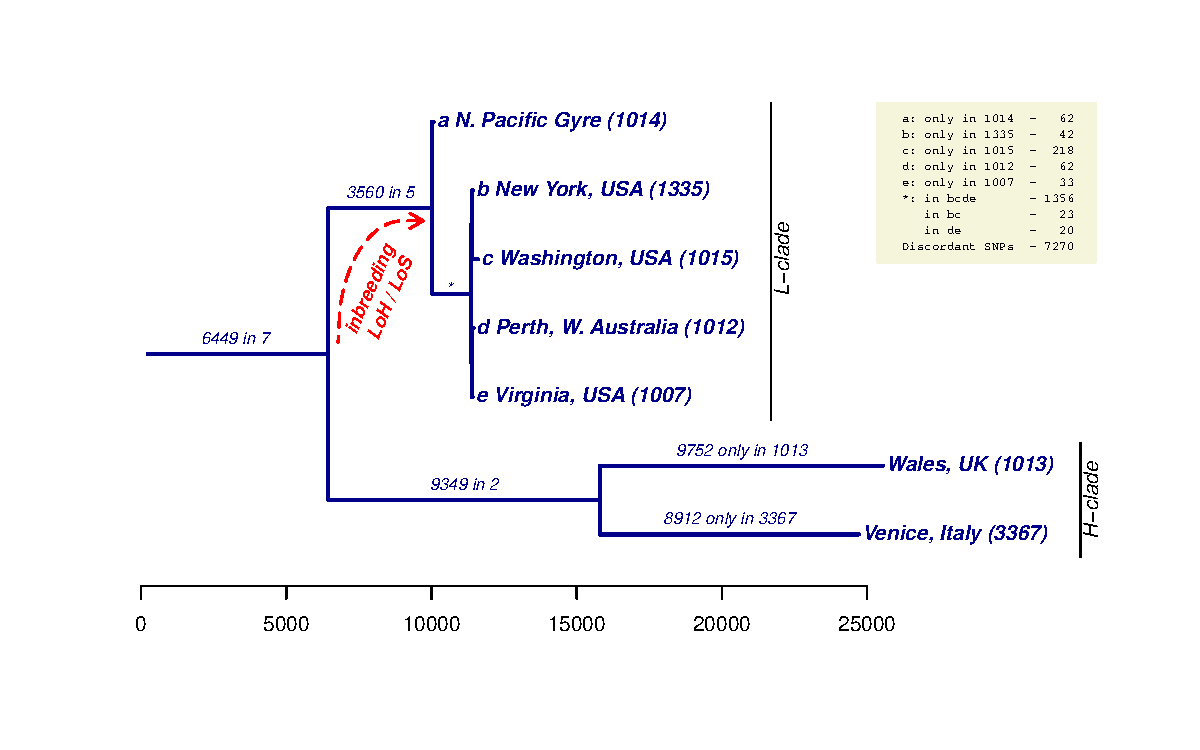
\includegraphics{figs-mine/paperfig-medium-tree-Chr1-qfiltered.pdf}
  \caption{Proposed fig. for paper: Tree based on qfiltered reads and medium SNP filters.  ``Lengths'' are numbers of shared/private SNPs on Chr1.}
  \label{fig:tree-paper}
\end{figure}

\begin{knitrout}\scriptsize
\definecolor{shadecolor}{rgb}{0.969, 0.969, 0.969}\color{fgcolor}\begin{kframe}
\begin{alltt}
\hlcom{# fig.paths for knitr chunks below;  .h for "hand-made" trees; plain for automatic chr1/full versions}
\hlstd{myfigpath}   \hlkwb{<-} \hlkwd{paste}\hlstd{(}\hlkwd{getwd}\hlstd{(),} \hlstr{'/figs-knitr/newick-'}\hlstd{,} \hlkwd{which.snp.tables}\hlstd{(),} \hlstr{'-'}\hlstd{,} \hlkwc{sep}\hlstd{=}\hlstr{''}\hlstd{)}
\hlstd{myfigpath.h} \hlkwb{<-} \hlkwd{paste}\hlstd{(}\hlkwd{getwd}\hlstd{(),} \hlstr{'/figs-knitr/newick-'}\hlstd{,} \hlkwc{sep}\hlstd{=}\hlstr{''}\hlstd{)}
\end{alltt}
\end{kframe}
\end{knitrout}

Figure~\ref{fig:tree-loose}, i.e., criteria [[1]]:

\begin{knitrout}\scriptsize
\definecolor{shadecolor}{rgb}{0.969, 0.969, 0.969}\color{fgcolor}\begin{kframe}
\begin{alltt}
\hlstd{newick.loose} \hlkwb{<-} \hlkwd{newickize}\hlstd{(}\hlkwd{make.tree}\hlstd{(pat.summaries[,}\hlstr{'count1'}\hlstd{]))}
\hlkwd{show.tree}\hlstd{(newick.loose,} \hlkwc{total.snps}\hlstd{=consistent.count[}\hlnum{1}\hlstd{])}
\end{alltt}
\end{kframe}\begin{figure}

{\centering 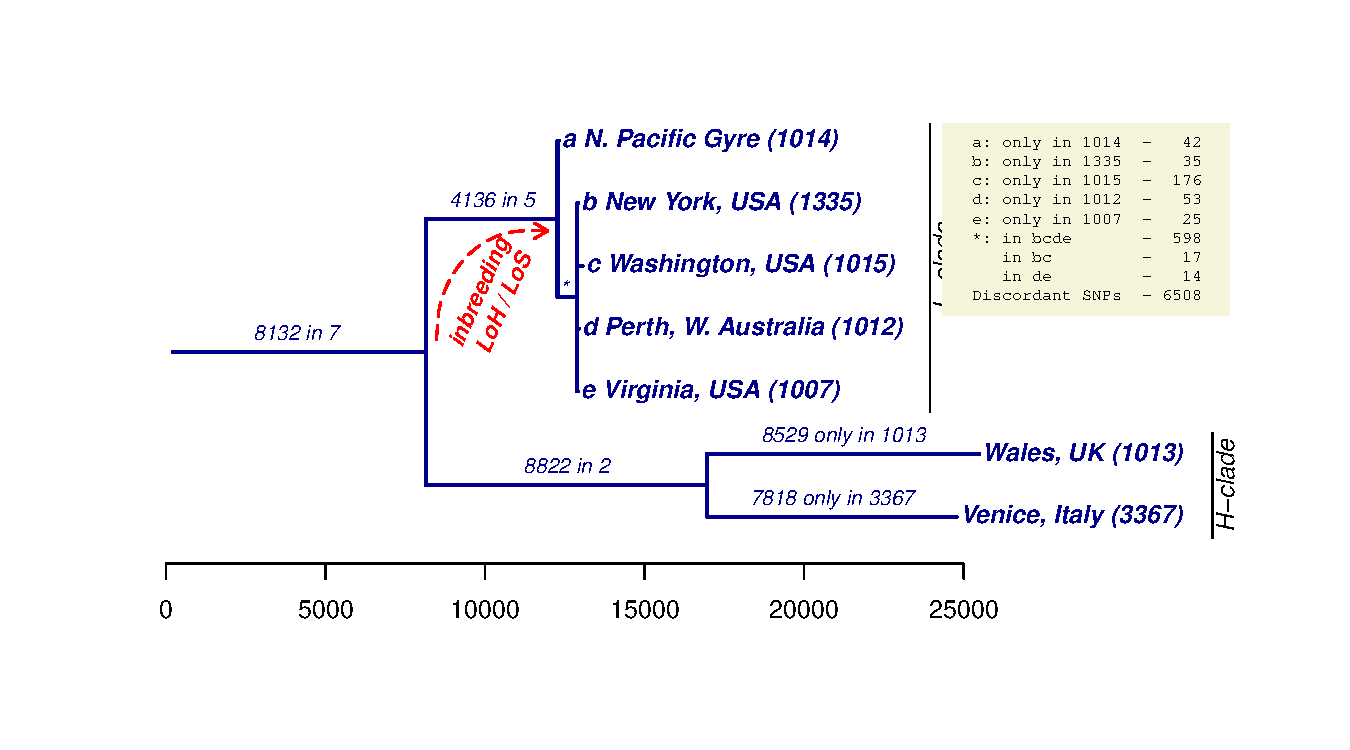
\includegraphics[width=\maxwidth]{/homes/gws/ruzzo/Documents/g/projects/thaps/Thaps_7_strains/scripts/larrys/shared-snps/figs-knitr/newick-Chr1-qfiltered-tree-loose-1} 

}

\caption[Tree based on qfiltered reads and loose SNP filters]{Tree based on qfiltered reads and loose SNP filters.  ``Lengths'' are numbers of shared/private SNPs on Chr1.}\label{fig:tree-loose}
\end{figure}


\end{knitrout}

Figure~\ref{fig:tree-medium}, i.e. [[2]]:

\begin{knitrout}\scriptsize
\definecolor{shadecolor}{rgb}{0.969, 0.969, 0.969}\color{fgcolor}\begin{kframe}
\begin{alltt}
\hlcom{# newick.medium <- newickize(tree.by.hand)}
\hlcom{# simple.newick.medium <- newickize(tree.by.hand,alt=TRUE)}
\hlstd{newick.medium} \hlkwb{<-} \hlkwd{newickize}\hlstd{(}\hlkwd{make.tree}\hlstd{(pat.summaries[,}\hlstr{'count2'}\hlstd{]))}
\hlstd{simple.newick.medium} \hlkwb{<-} \hlkwd{newickize}\hlstd{(}\hlkwd{make.tree}\hlstd{(pat.summaries[,}\hlstr{'count2'}\hlstd{]),}\hlkwc{alt}\hlstd{=}\hlnum{TRUE}\hlstd{)}
\hlkwd{show.tree}\hlstd{(newick.medium,} \hlkwc{total.snps}\hlstd{=consistent.count[}\hlnum{2}\hlstd{])}
\end{alltt}
\end{kframe}\begin{figure}

{\centering 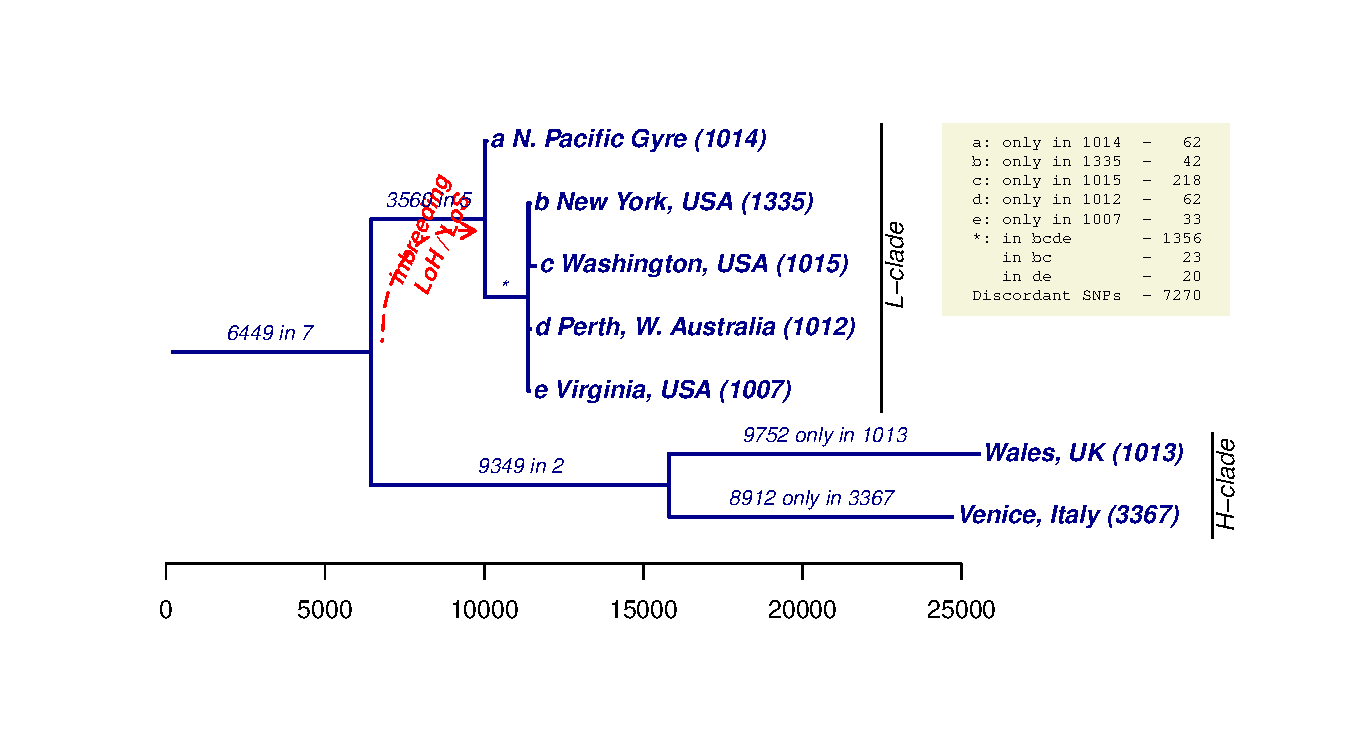
\includegraphics[width=\maxwidth]{/homes/gws/ruzzo/Documents/g/projects/thaps/Thaps_7_strains/scripts/larrys/shared-snps/figs-knitr/newick-Chr1-qfiltered-tree-medium-1} 

}

\caption[Tree based on qfiltered reads and medium SNP filters]{Tree based on qfiltered reads and medium SNP filters.  ``Lengths'' are numbers of shared/private SNPs on Chr1.}\label{fig:tree-medium}
\end{figure}


\end{knitrout}

Figure~\ref{fig:tree-strict}, i.e. [[3]]:

\begin{knitrout}\scriptsize
\definecolor{shadecolor}{rgb}{0.969, 0.969, 0.969}\color{fgcolor}\begin{kframe}
\begin{alltt}
\hlstd{newick.strict} \hlkwb{<-} \hlkwd{newickize}\hlstd{(}\hlkwd{make.tree}\hlstd{(pat.summaries[,}\hlstr{'count3'}\hlstd{]))}
\hlkwd{show.tree}\hlstd{(newick.strict,} \hlkwc{total.snps}\hlstd{=consistent.count[}\hlnum{3}\hlstd{])}
\end{alltt}
\end{kframe}\begin{figure}

{\centering 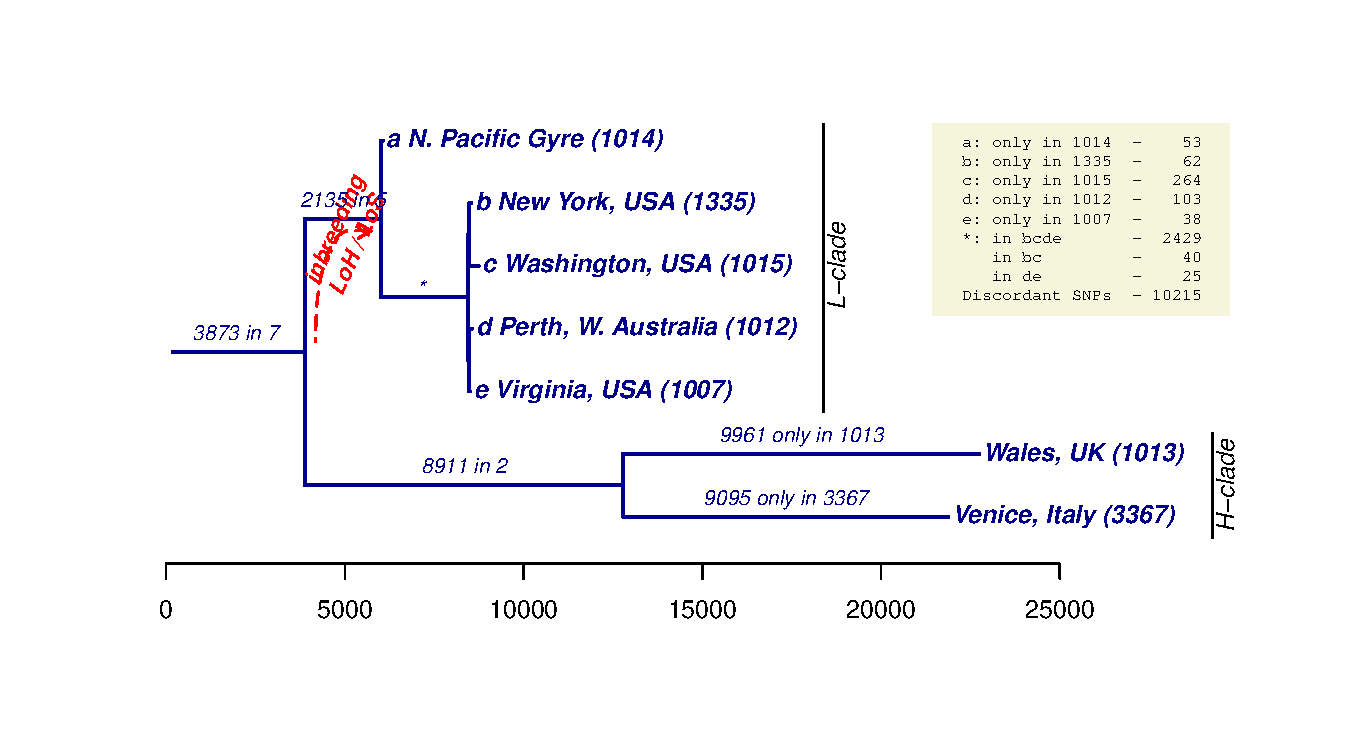
\includegraphics[width=\maxwidth]{/homes/gws/ruzzo/Documents/g/projects/thaps/Thaps_7_strains/scripts/larrys/shared-snps/figs-knitr/newick-Chr1-qfiltered-tree-strict-1} 

}

\caption[Tree based on qfiltered reads and strict SNP filters]{Tree based on qfiltered reads and strict SNP filters.  ``Lengths'' are numbers of shared/private SNPs on Chr1.}\label{fig:tree-strict}
\end{figure}


\end{knitrout}

Figure~\ref{fig:tree-unfiltered}, i.e. [[4]]:

\begin{knitrout}\scriptsize
\definecolor{shadecolor}{rgb}{0.969, 0.969, 0.969}\color{fgcolor}\begin{kframe}
\begin{alltt}
\hlstd{newick.unfiltered} \hlkwb{<-} \hlkwd{newickize}\hlstd{(}\hlkwd{make.tree}\hlstd{(pat.summaries[,}\hlstr{'count4'}\hlstd{]))}
\hlkwd{show.tree}\hlstd{(newick.unfiltered,} \hlkwc{total.snps}\hlstd{=consistent.count[}\hlnum{4}\hlstd{])}
\end{alltt}
\end{kframe}\begin{figure}

{\centering 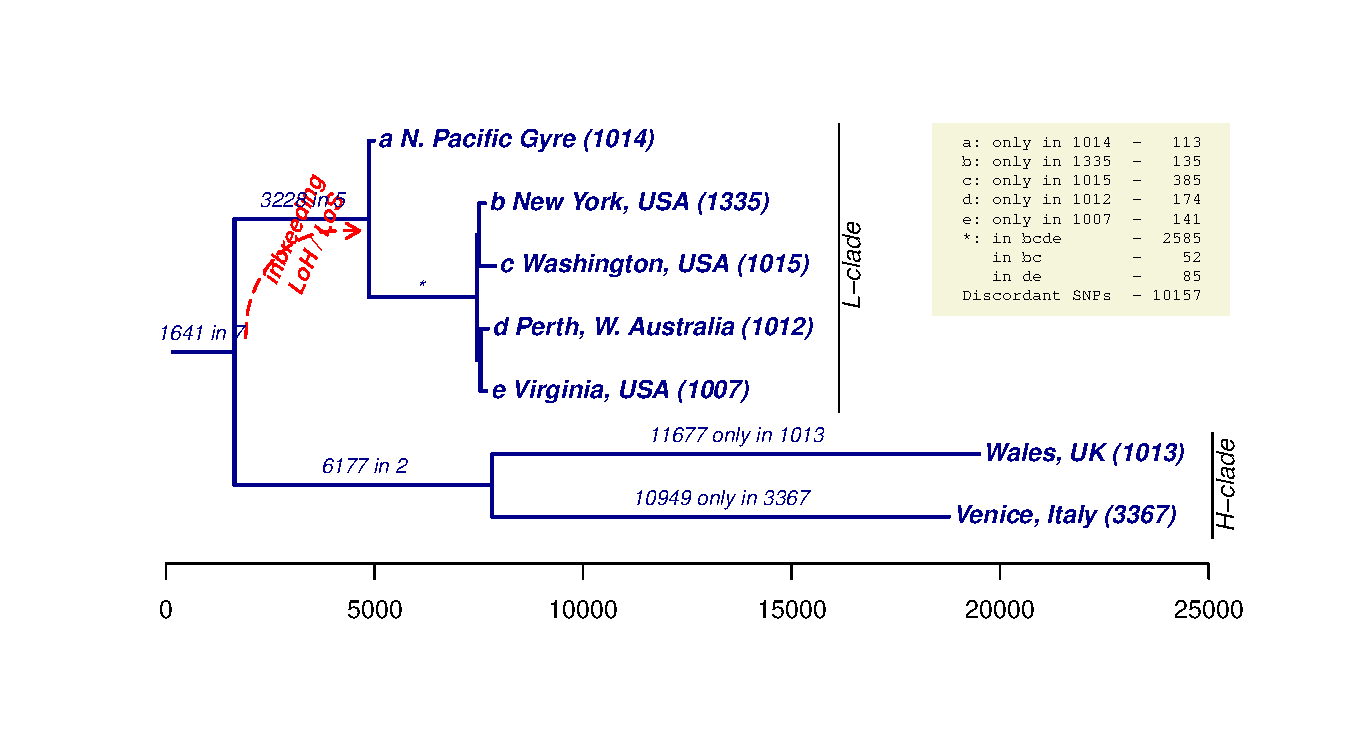
\includegraphics[width=\maxwidth]{/homes/gws/ruzzo/Documents/g/projects/thaps/Thaps_7_strains/scripts/larrys/shared-snps/figs-knitr/newick-Chr1-qfiltered-tree-unfiltered-1} 

}

\caption[Tree based on qfiltered reads and unfiltered SNPs]{Tree based on qfiltered reads and unfiltered SNPs.  ``Lengths'' are numbers of shared/private SNPs on Chr1.}\label{fig:tree-unfiltered}
\end{figure}


\end{knitrout}

Some other versions of the trees are included in the appendix.

Counts for all tree edges in the medium tree: 

\begin{knitrout}\scriptsize
\definecolor{shadecolor}{rgb}{0.969, 0.969, 0.969}\color{fgcolor}\begin{kframe}
\begin{alltt}
\hlcom{#pat.summaries[c(128,110,102,6,97,19,9,2,5,33,65,17,3),]}
\hlstd{tree.edges} \hlkwb{<-} \hlkwd{c}\hlstd{(}\hlnum{128}\hlstd{,}\hlnum{110}\hlstd{,}\hlnum{102}\hlstd{,}\hlnum{6}\hlstd{,}\hlnum{97}\hlstd{,}\hlnum{19}\hlstd{,}\hlnum{9}\hlstd{,}\hlnum{2}\hlstd{,}\hlnum{5}\hlstd{,}\hlnum{33}\hlstd{,}\hlnum{65}\hlstd{,}\hlnum{17}\hlstd{,}\hlnum{3}\hlstd{)}\hlopt{-}\hlnum{1}
\hlstd{non.edges} \hlkwb{<-} \hlkwd{setdiff}\hlstd{(}\hlnum{0}\hlopt{:}\hlnum{127}\hlstd{, tree.edges)}
\hlstd{sg.edges} \hlkwb{<-} \hlkwd{showgroup}\hlstd{(}\hlkwc{restrict.to}\hlstd{=tree.edges) ; sg.edges}
\end{alltt}
\begin{verbatim}
#       Pat ShrBy 1007 1012 1013 1014 1015 3367 1335 count1 count2 count3 count4
# 2     001     1                                  X     35     42     62    135
# 3     002     1                             X        7818   8912   9095  10949
# 5     004     1                        X              176    218    264    385
# 6     005     2                        X         X     17     23     40     52
# 9     010     1                   X                    42     62     53    113
# 17    020     1              X                       8529   9752   9961  11677
# 19    022     2              X              X        8822   9349   8911   6177
# 33    040     1         X                              53     62    103    174
# 65    100     1    X                                   25     33     38    141
# 97    140     2    X    X                              14     20     25     85
# 102   145     4    X    X              X         X    598   1356   2429   2585
# 110   155     5    X    X         X    X         X   4136   3560   2135   3228
# 128   177     7    X    X    X    X    X    X    X   8132   6449   3873   1641
# Total                                               38397  39838  36989  37342
\end{verbatim}
\end{kframe}
\end{knitrout}

Counts for the top 10 discordant patterns, i.e., SNPs whose sharing pattern does not match any of the bifurcations in the tree:

\begin{knitrout}\scriptsize
\definecolor{shadecolor}{rgb}{0.969, 0.969, 0.969}\color{fgcolor}\begin{kframe}
\begin{alltt}
\hlstd{tenth} \hlkwb{<-} \hlkwd{sort}\hlstd{(}\hlkwd{showgroup}\hlstd{(}\hlkwc{restrict.to}\hlstd{=non.edges)[}\hlopt{-}\hlstd{(}\hlkwd{length}\hlstd{(non.edges)}\hlopt{+}\hlnum{1}\hlstd{),}\hlstr{'count2'}\hlstd{],}\hlkwc{decreasing}\hlstd{=T)[}\hlnum{10}\hlstd{]}
\hlstd{sg.non.edges} \hlkwb{<-} \hlkwd{showgroup}\hlstd{(}\hlkwc{restrict.to}\hlstd{=non.edges,} \hlkwc{c2.thresh} \hlstd{= tenth) ; sg.non.edges}
\end{alltt}
\begin{verbatim}
#       Pat ShrBy 1007 1012 1013 1014 1015 3367 1335 count1 count2 count3 count4
# 1     000     0                                         9     51    468      0
# 56    067     5         X    X         X    X    X     48    109    257    104
# 101   144     3    X    X              X               18     74    159    355
# 104   147     5    X    X              X    X    X    205    421    740   1160
# 112   157     6    X    X         X    X    X    X   1338   1076    665   1343
# 117   164     4    X    X    X         X               19     51     71    163
# 118   165     5    X    X    X         X         X    318    591    957   1140
# 119   166     5    X    X    X         X    X          46    154    220    254
# 120   167     6    X    X    X         X    X    X   1305   2445   4098   1852
# 126   175     6    X    X    X    X    X         X   1709   1352    834   1416
# 127   176     6    X    X    X    X    X    X          57     79     43     68
# Other   (   104 rows   w/   c2    <   51    )        1436    867   1703   2302
# Total                                                6508   7270  10215  10157
\end{verbatim}
\end{kframe}
\end{knitrout}

And percent of discordant SNPs:

\begin{knitrout}\scriptsize
\definecolor{shadecolor}{rgb}{0.969, 0.969, 0.969}\color{fgcolor}\begin{kframe}
\begin{alltt}
\hlstd{nsge} \hlkwb{<-} \hlkwd{nrow}\hlstd{(sg.edges)}
\hlstd{discordv} \hlkwb{<-} \hlstd{consistent.count} \hlopt{-} \hlstd{sg.edges[nsge,}\hlkwd{c}\hlstd{(}\hlstr{'count1'}\hlstd{,}\hlstr{'count2'}\hlstd{,}\hlstr{'count3'}\hlstd{,}\hlstr{'count4'}\hlstd{)] ; discordv}
\end{alltt}
\begin{verbatim}
#       count1 count2 count3 count4
# Total   6508   7270  10215  10157
\end{verbatim}
\begin{alltt}
\hlstd{discordv.pct} \hlkwb{<-} \hlkwd{round}\hlstd{(discordv}\hlopt{/}\hlstd{consistent.count}\hlopt{*}\hlnum{100}\hlstd{,}\hlnum{1}\hlstd{) ; discordv.pct}
\end{alltt}
\begin{verbatim}
#       count1 count2 count3 count4
# Total   14.5   15.4   21.6   21.4
\end{verbatim}
\end{kframe}
\end{knitrout}

In short, the sharing pattern observed at 7270 or 15.4\% of the 
47108 medium-stringency consistent SNPs positions observed across all 7 
isolates are discordant with the medium tree.  (The strict tree has slightly more.)  

A majority of the discordant SNPs fall into one of three patterns: 6-way sharing excluding Gyre 
(likely a technical artifact since the low coverage in Gyre reduces our power to detect SNPs there), 
or 6-way sharing excluding one of the two H-isolates (likely a reflection of sexuality in the 
H-clade---SNP positions in a population in Hardy-Weinberg equilibrium are fairly likely to be 
homozygous for the reference allele in a given individual).

\begin{knitrout}\scriptsize
\definecolor{shadecolor}{rgb}{0.969, 0.969, 0.969}\color{fgcolor}\begin{kframe}
\begin{alltt}
\hlstd{third.biggest} \hlkwb{<-} \hlkwd{sort}\hlstd{(}\hlkwd{showgroup}\hlstd{(pat.summaries,}\hlnum{6}\hlstd{)[}\hlopt{-}\hlnum{8}\hlstd{,}\hlstr{'count2'}\hlstd{],}\hlkwc{decreasing}\hlstd{=T)[}\hlnum{3}\hlstd{]}
\hlstd{big.three} \hlkwb{<-} \hlkwd{showgroup}\hlstd{(pat.summaries,}\hlnum{6}\hlstd{,}\hlkwc{c2.thresh} \hlstd{= third.biggest); big.three}
\end{alltt}
\begin{verbatim}
#       Pat ShrBy 1007 1012 1013 1014 1015 3367 1335 count1 count2 count3 count4
# 112   157     6    X    X         X    X    X    X   1338   1076    665   1343
# 120   167     6    X    X    X         X    X    X   1305   2445   4098   1852
# 126   175     6    X    X    X    X    X         X   1709   1352    834   1416
# Other   (     4 rows   w/   c2    < 1076    )         123    136    118    111
# Total                                                4475   5009   5715   4722
\end{verbatim}
\begin{alltt}
\hlstd{big.three.frac} \hlkwb{<-} \hlkwd{sum}\hlstd{(big.three[}\hlnum{1}\hlopt{:}\hlnum{3}\hlstd{,}\hlstr{'count2'}\hlstd{])}\hlopt{/}\hlstd{discordv}\hlopt{$}\hlstd{count2; big.three.frac}
\end{alltt}
\begin{verbatim}
# [1] 0.6702889
\end{verbatim}
\end{kframe}
\end{knitrout}

\noindent I.e., 67\% of discordant SNPs fall into one of these three 
categories.

Out of curiousity: what is the ratio of full genome to Chr 1 branch lengths.  Except for the shortest 
few, generally $\approx$10x, as expected given the length of Chr 1:

\begin{knitrout}\scriptsize
\definecolor{shadecolor}{rgb}{0.969, 0.969, 0.969}\color{fgcolor}\begin{kframe}
\begin{alltt}
\hlcom{# (vectors derived by editing Newick strings, and in that order)}
\hlkwd{print}\hlstd{(}
  \hlkwd{c}\hlstd{(}\hlkwc{Italy}\hlstd{=}\hlnum{86155}\hlstd{,} \hlkwc{Wales}\hlstd{=}\hlnum{95697}\hlstd{,} \hlkwc{IW}\hlstd{=}\hlnum{89598}\hlstd{,} \hlkwc{Virg}\hlstd{=}\hlnum{330}\hlstd{,}     \hlkwc{Aust}\hlstd{=}\hlnum{632}\hlstd{,}      \hlkwc{VA}\hlstd{=}\hlnum{1296}\hlstd{,}
    \hlkwc{Puget}\hlstd{=}\hlnum{2113}\hlstd{,}  \hlkwc{NY}\hlstd{=}\hlnum{658}\hlstd{,}      \hlkwc{PNY}\hlstd{=}\hlnum{480}\hlstd{,}  \hlkwc{four}\hlstd{=}\hlnum{10059}\hlstd{,}   \hlkwc{Gyre}\hlstd{=}\hlnum{568}\hlstd{,}      \hlkwc{five}\hlstd{=}\hlnum{39517}\hlstd{,} \hlkwc{all}\hlstd{=}\hlnum{69526}\hlstd{)} \hlopt{/}
  \hlkwd{c}\hlstd{(}\hlkwc{Italy}\hlstd{=}\hlnum{8813}\hlstd{,}  \hlkwc{Wales}\hlstd{=}\hlnum{9652}\hlstd{,}  \hlkwc{IW}\hlstd{=}\hlnum{9365}\hlstd{,}  \hlkwc{Virg}\hlstd{=}\hlnum{30}\hlstd{,}      \hlkwc{Aust}\hlstd{=}\hlnum{61}\hlstd{,}       \hlkwc{VA}\hlstd{=}\hlnum{19}\hlstd{,}
    \hlkwc{Puget}\hlstd{=}\hlnum{207}\hlstd{,}   \hlkwc{NY}\hlstd{=}\hlnum{41}\hlstd{,}       \hlkwc{PNY}\hlstd{=}\hlnum{18}\hlstd{,}   \hlkwc{four}\hlstd{=}\hlnum{1005}\hlstd{,}    \hlkwc{Gyre}\hlstd{=}\hlnum{61}\hlstd{,}       \hlkwc{five}\hlstd{=}\hlnum{3912}\hlstd{,}  \hlkwc{all}\hlstd{=} \hlnum{7054}\hlstd{),}
  \hlkwc{digits}\hlstd{=}\hlnum{3}\hlstd{)}
\end{alltt}
\begin{verbatim}
# Italy Wales    IW  Virg  Aust    VA Puget    NY   PNY  four  Gyre  five   all 
#  9.78  9.91  9.57 11.00 10.36 68.21 10.21 16.05 26.67 10.01  9.31 10.10  9.86
\end{verbatim}
\begin{alltt}
\hlkwd{round}\hlstd{(}\hlkwd{genome.length.constants}\hlstd{()}\hlopt{$}\hlstd{genome.length.trunc} \hlopt{/} \hlkwd{genome.length.constants}\hlstd{()}\hlopt{$}\hlstd{chr1.length,} \hlkwc{digits}\hlstd{=}\hlnum{4}\hlstd{)}
\end{alltt}
\begin{verbatim}
# [1] 10.2879
\end{verbatim}
\end{kframe}
\end{knitrout}

\section{Semi-Automated Tree-Building}
Slightly formalizing the process above: Look for the bifurcation of the 7 strains that maximizes the 
number of shared SNPs \emph{within} each side of the partition while minimizing the number and 
fraction of SNPs that are shared by subsets that include at least one strain on each side of the 
partition.  The 2/5 split is the winner, with 6418 SNPs in confict with that partition (16\% of the 
39842 SNPs not shared by all 7; Chr1 data).  The runner-up places the Gyre in a group by
itself (7079 = 18\% in conflict).

\begin{knitrout}\footnotesize
\definecolor{shadecolor}{rgb}{0.969, 0.969, 0.969}\color{fgcolor}\begin{kframe}
\begin{alltt}
\hlstd{treepart} \hlkwb{<-} \hlkwa{function}\hlstd{(}\hlkwc{p.summ}\hlstd{=pat.summaries,} \hlkwc{root}\hlstd{=}\hlnum{127}\hlstd{,} \hlkwc{verbose}\hlstd{=T,} \hlkwc{stringency}\hlstd{=}\hlstr{'count2'}\hlstd{)\{}
  \hlstd{root.shared} \hlkwb{<-} \hlstd{p.summ[root}\hlopt{+}\hlnum{1}\hlstd{,stringency]}
  \hlstd{df}\hlkwb{<-}\hlkwa{NULL}
  \hlkwa{for}\hlstd{(i} \hlkwa{in} \hlnum{1}\hlopt{:}\hlkwd{floor}\hlstd{(root}\hlopt{/}\hlnum{2}\hlstd{))\{}
    \hlkwa{if}\hlstd{(}\hlkwd{bitwAnd}\hlstd{(i,root)}\hlopt{==}\hlstd{i} \hlopt{&&} \hlstd{i} \hlopt{<} \hlstd{root}\hlopt{-}\hlstd{i)\{}
      \hlstd{l1} \hlkwb{<-} \hlkwd{showgroup}\hlstd{(p.summ,}\hlkwc{subset}\hlstd{=i,}\hlkwc{split}\hlstd{=}\hlkwa{NULL}\hlstd{,}\hlkwc{proper.subset}\hlstd{=F,}\hlkwc{total}\hlstd{=T)}
      \hlstd{l}  \hlkwb{<-} \hlstd{l1[}\hlkwd{nrow}\hlstd{(l1),stringency]}
      \hlstd{r1} \hlkwb{<-} \hlkwd{showgroup}\hlstd{(p.summ,}\hlkwc{subset}\hlstd{=root}\hlopt{-}\hlstd{i,}\hlkwc{split}\hlstd{=}\hlkwa{NULL}\hlstd{,}\hlkwc{proper.subset}\hlstd{=F,}\hlkwc{total}\hlstd{=T)}
      \hlstd{r}  \hlkwb{<-} \hlstd{r1[}\hlkwd{nrow}\hlstd{(r1),stringency]}
      \hlstd{c1} \hlkwb{<-} \hlkwd{showgroup}\hlstd{(p.summ,}\hlkwc{subset}\hlstd{=root,}\hlkwc{split}\hlstd{=i,}\hlkwc{proper.subset}\hlstd{=T,}\hlkwc{total}\hlstd{=T)}
      \hlstd{c}  \hlkwb{<-} \hlstd{c1[}\hlkwd{nrow}\hlstd{(c1),stringency]}
      \hlstd{df} \hlkwb{<-} \hlkwd{rbind}\hlstd{(df,} \hlkwd{data.frame}\hlstd{(}\hlkwc{pat}\hlstd{=i,}\hlkwc{left}\hlstd{=l,}\hlkwc{right}\hlstd{=r,}\hlkwc{both}\hlstd{=l}\hlopt{+}\hlstd{r,}\hlkwc{cross}\hlstd{=c,}\hlkwc{all}\hlstd{=l}\hlopt{+}\hlstd{r}\hlopt{+}\hlstd{c,}\hlkwc{ratio}\hlstd{=c}\hlopt{/}\hlstd{(l}\hlopt{+}\hlstd{r}\hlopt{+}\hlstd{c),}
                                 \hlkwc{best}\hlstd{=}\hlstr{''}\hlstd{,}\hlkwc{stringsAsFactors}\hlstd{=F))}
    \hlstd{\}}
  \hlstd{\}}
  \hlstd{df}\hlopt{$}\hlstd{pat}\hlkwb{<-}\hlkwd{as.octmode}\hlstd{(df}\hlopt{$}\hlstd{pat)}
  \hlstd{maxl} \hlkwb{<-} \hlkwd{which.max}\hlstd{(df}\hlopt{$}\hlstd{left)}
  \hlstd{maxr} \hlkwb{<-} \hlkwd{which.max}\hlstd{(df}\hlopt{$}\hlstd{right)}
  \hlstd{maxb} \hlkwb{<-} \hlkwd{which.max}\hlstd{(df}\hlopt{$}\hlstd{both)}
  \hlstd{minc} \hlkwb{<-} \hlkwd{which.min}\hlstd{(df}\hlopt{$}\hlstd{cross)}
  \hlstd{minr} \hlkwb{<-} \hlkwd{which.min}\hlstd{(df}\hlopt{$}\hlstd{ratio)}
  \hlstd{df}\hlopt{$}\hlstd{best[}\hlkwd{c}\hlstd{(maxl,maxr,maxb,minc,minr)]} \hlkwb{<-} \hlstr{'<'}
  \hlstd{df}\hlopt{$}\hlstd{best[maxl]} \hlkwb{<-} \hlkwd{paste}\hlstd{(df}\hlopt{$}\hlstd{best[maxl],} \hlstr{'L'}\hlstd{)} \hlcom{# max Left}
  \hlstd{df}\hlopt{$}\hlstd{best[maxr]} \hlkwb{<-} \hlkwd{paste}\hlstd{(df}\hlopt{$}\hlstd{best[maxr],} \hlstr{'R'}\hlstd{)} \hlcom{# max Right}
  \hlstd{df}\hlopt{$}\hlstd{best[maxb]} \hlkwb{<-} \hlkwd{paste}\hlstd{(df}\hlopt{$}\hlstd{best[maxb],} \hlstr{'B'}\hlstd{)} \hlcom{# max Both (L+R)}
  \hlstd{df}\hlopt{$}\hlstd{best[minc]} \hlkwb{<-} \hlkwd{paste}\hlstd{(df}\hlopt{$}\hlstd{best[minc],} \hlstr{'C'}\hlstd{)} \hlcom{# min Cross}
  \hlstd{df}\hlopt{$}\hlstd{best[minr]} \hlkwb{<-} \hlkwd{paste}\hlstd{(df}\hlopt{$}\hlstd{best[minr],} \hlstr{'O'}\hlstd{)} \hlcom{# min ratiO (Cross/(Left+Right+Cross)}
  \hlkwa{if}\hlstd{(verbose)\{}
    \hlstd{same} \hlkwb{<-} \hlkwd{all}\hlstd{(maxl}\hlopt{==}\hlkwd{c}\hlstd{(maxr,maxb,minc,minr))}
    \hlkwd{cat}\hlstd{(}\hlstr{'root:'}\hlstd{,}       \hlkwd{format}\hlstd{(}\hlkwd{as.octmode}\hlstd{(root),}\hlkwc{width}\hlstd{=}\hlnum{3}\hlstd{),}
        \hlstr{'; shared:'}\hlstd{,   root.shared,}
        \hlstr{'.  max l'}\hlstd{,}    \hlkwd{format}\hlstd{(}\hlkwd{as.octmode}\hlstd{(df}\hlopt{$}\hlstd{pat[maxl]),}\hlkwc{width}\hlstd{=}\hlnum{3}\hlstd{),}
        \hlstr{', max r'}\hlstd{,}     \hlkwd{format}\hlstd{(}\hlkwd{as.octmode}\hlstd{(df}\hlopt{$}\hlstd{pat[maxr]),}\hlkwc{width}\hlstd{=}\hlnum{3}\hlstd{),}
        \hlstr{', max both'}\hlstd{,}  \hlkwd{format}\hlstd{(}\hlkwd{as.octmode}\hlstd{(df}\hlopt{$}\hlstd{pat[maxb]),}\hlkwc{width}\hlstd{=}\hlnum{3}\hlstd{),}
        \hlstr{', min cross'}\hlstd{,} \hlkwd{format}\hlstd{(}\hlkwd{as.octmode}\hlstd{(df}\hlopt{$}\hlstd{pat[minc]),}\hlkwc{width}\hlstd{=}\hlnum{3}\hlstd{),}
        \hlstr{', min ratio'}\hlstd{,} \hlkwd{format}\hlstd{(}\hlkwd{as.octmode}\hlstd{(df}\hlopt{$}\hlstd{pat[minr]),}\hlkwc{width}\hlstd{=}\hlnum{3}\hlstd{),}
        \hlstr{'. \textbackslash{}nAll the same?:'}\hlstd{,same,}
        \hlstr{'\textbackslash{}n'}\hlstd{)}
    \hlkwd{cat}\hlstd{(}\hlstr{'\textbackslash{}n'}\hlstd{)}
  \hlstd{\}}
  \hlkwd{return}\hlstd{(df)}
\hlstd{\}}
\end{alltt}
\end{kframe}
\end{knitrout}

\begin{knitrout}\footnotesize
\definecolor{shadecolor}{rgb}{0.969, 0.969, 0.969}\color{fgcolor}\begin{kframe}
\begin{alltt}
\hlkwd{treepart}\hlstd{()}
\end{alltt}
\begin{verbatim}
# root: 177 ; shared: 6449 .  max l 077 , max r 010 , max both 010 , min cross 010 , min ratio 010 . 
# All the same?: FALSE
#    pat  left right  both cross   all     ratio      best
# 1   01    93 29241 29334 11376 40710 0.2794399          
# 2   02  8963 17601 26564 14146 40710 0.3474822          
# 3   03  9020 10496 19516 21194 40710 0.5206092          
# 4   04   269 28545 28814 11896 40710 0.2922132          
# 5   05   334 28340 28674 12036 40710 0.2956522          
# 6   06  9190 10106 19296 21414 40710 0.5260133          
# 7   07  9273 10006 19279 21431 40710 0.5264309          
# 8   10   113 34247 34360  6350 40710 0.1559813 < R B C O
# 9   11   160 28961 29121 11589 40710 0.2846721          
# 10  12  9029 12483 21512 19198 40710 0.4715795          
# 11  13  9093 10343 19436 21274 40710 0.5225743          
# 12  14   332 28414 28746 11964 40710 0.2938836          
# 13  15   406 28242 28648 12062 40710 0.2962908          
# 14  16  9257 10017 19274 21436 40710 0.5265537          
# 15  17  9353  9934 19287 21423 40710 0.5262343          
# 16  20  9803 16282 26085 14625 40710 0.3592483          
# 17  21  9852  9610 19462 21248 40710 0.5219356          
# 18  22 28064  5697 33761  6949 40710 0.1706952          
# 19  23 28151   607 28758 11952 40710 0.2935888          
# 20  24 10036  9264 19300 21410 40710 0.5259150          
# 21  25 10112  9160 19272 21438 40710 0.5266028          
# 22  26 28337   301 28638 12072 40710 0.2965365          
# 23  27 28470   231 28701 12009 40710 0.2949889          
# 24  30  9870 11459 21329 19381 40710 0.4760747          
# 25  31  9925  9471 19396 21314 40710 0.5235569          
# 26  32 28144  1982 30126 10584 40710 0.2599853          
# 27  33 28241   485 28726 11984 40710 0.2943748          
# 28  34 10109  9178 19287 21423 40710 0.5262343          
# 29  35 10199  9087 19286 21424 40710 0.5262589          
# 30  36 28423   226 28649 12061 40710 0.2962663          
# 31  37 28587   166 28753 11957 40710 0.2937116          
# 32  40   113 28782 28895 11815 40710 0.2902235          
# 33  41   159 28529 28688 12022 40710 0.2953083          
# 34  42  9027 10293 19320 21390 40710 0.5254237          
# 35  43  9098 10173 19271 21439 40710 0.5266274          
# 36  44   348 28314 28662 12048 40710 0.2959469          
# 37  45   461 28196 28657 12053 40710 0.2960698          
# 38  46  9283  9971 19254 21456 40710 0.5270450          
# 39  47  9450  9910 19360 21350 40710 0.5244412          
# 40  50   176 28634 28810 11900 40710 0.2923115          
# 41  51   229 28429 28658 12052 40710 0.2960452          
# 42  52  9094 10190 19284 21426 40710 0.5263080          
# 43  53  9175 10091 19266 21444 40710 0.5267502          
# 44  54   419 28216 28635 12075 40710 0.2966102          
# 45  55   558 28112 28670 12040 40710 0.2957504          
# 46  56  9360  9895 19255 21455 40710 0.5270204          
# 47  57  9567  9841 19408 21302 40710 0.5232621          
# 48  60  9873  9454 19327 21383 40710 0.5252518          
# 49  61  9934  9320 19254 21456 40710 0.5270450          
# 50  62 28157   478 28635 12075 40710 0.2966102          
# 51  63 28278   380 28658 12052 40710 0.2960452          
# 52  64 10140  9141 19281 21429 40710 0.5263817          
# 53  65 10293  9068 19361 21349 40710 0.5244166          
# 54  66 28519   200 28719 11991 40710 0.2945468          
# 55  67 28886   147 29033 11677 40710 0.2868337          
# 56  70  9941  9362 19303 21407 40710 0.5258413          
# 57  71 10012  9247 19259 21451 40710 0.5269221          
# 58  72 28240   396 28636 12074 40710 0.2965856          
# 59  73 28379   312 28691 12019 40710 0.2952346          
# 60  74 10223  9065 19288 21422 40710 0.5262098          
# 61  75 10416  9000 19416 21294 40710 0.5230656          
# 62  76 28629   131 28760 11950 40710 0.2935397          
# 63  77 29112    84 29196 11514 40710 0.2828298       < L
\end{verbatim}
\end{kframe}
\end{knitrout}

Comparing the 5/2 split to the second-place NPG/rest split (below), the former has fewer pattern instances in conflict
with the split (6418 vs 7079), as well as somewhat more random distribution of the conflicting patterns (92 vs 62 rows),
whereas the 1/6 split has the majority of its conflicts (3912 of 7079, or 55\%) concentrated in one pattern---the 5 NE
strains.  Collectively, these seem to favor the 5/2 split as the correct ``history.''

\begin{knitrout}\footnotesize
\definecolor{shadecolor}{rgb}{0.969, 0.969, 0.969}\color{fgcolor}\begin{kframe}
\begin{alltt}
\hlkwd{showgroup}\hlstd{(pat.summaries,}\hlkwc{split}\hlstd{=}\hlkwd{strtoi}\hlstd{(}\hlstr{'022'}\hlstd{),} \hlkwc{subset}\hlstd{=}\hlnum{127}\hlstd{,} \hlkwc{proper.subset}\hlstd{=T,} \hlkwc{c2.thresh}\hlstd{=}\hlnum{100}\hlstd{)}
\end{alltt}
\begin{verbatim}
#       Pat ShrBy 1007 1012 1013 1014 1015 3367 1335 count1 count2 count3 count4
# 56    067     5         X    X         X    X    X     48    109    257    104
# 104   147     5    X    X              X    X    X    205    421    740   1160
# 112   157     6    X    X         X    X    X    X   1338   1076    665   1343
# 118   165     5    X    X    X         X         X    318    591    957   1140
# 119   166     5    X    X    X         X    X          46    154    220    254
# 120   167     6    X    X    X         X    X    X   1305   2445   4098   1852
# 126   175     6    X    X    X    X    X         X   1709   1352    834   1416
# Other   (    85 rows   w/   c2    <  100    )        1415    801   1317   1735
# Total                                                6384   6949   9088   9004
\end{verbatim}
\begin{alltt}
\hlkwd{showgroup}\hlstd{(pat.summaries,}\hlkwc{split}\hlstd{=}\hlkwd{strtoi}\hlstd{(}\hlstr{'010'}\hlstd{),} \hlkwc{subset}\hlstd{=}\hlnum{127}\hlstd{,} \hlkwc{proper.subset}\hlstd{=T,} \hlkwc{c2.thresh}\hlstd{=}\hlnum{100}\hlstd{)}
\end{alltt}
\begin{verbatim}
#       Pat ShrBy 1007 1012 1013 1014 1015 3367 1335 count1 count2 count3 count4
# 110   155     5    X    X         X    X         X   4136   3560   2135   3228
# 112   157     6    X    X         X    X    X    X   1338   1076    665   1343
# 126   175     6    X    X    X    X    X         X   1709   1352    834   1416
# Other   (    59 rows   w/   c2    <  100    )         470    362    335    590
# Total                                                7653   6350   3969   6577
\end{verbatim}
\end{kframe}
\end{knitrout}

Below is the full summary of shared SNPs that do \emph{not} directly correspond to tree splits, e.g. deep coalescence, independent coincident mutations, false positives/false negatives in the shared SNP calls, loss of SNPs in hemizygous regions, etc.  (Additionally, SAMTools' SNP calls exclude positions it judges to be homozygous, and I think it operates without regard to the reference sequence, so homozygous nonreference positions, while rare except in IT/Wales, often are not called SNPs by SAMTools, but are relevant for this analysis.  Provided the position is called a SNP in some other isolate, the consistency filtering we've done above should recover it, but this is still worth keeping in mind when examining the data.) 

First, here are SNPs that ``coalesce'' on the branch from the LCA of bcde, i.e., shared among some nonempty, proper subset of bcde other than bc or de.  There are 8 such patterns: any of the 4 choose 3 trios plus any of the 4 pairs having exactly one of bc. 

\begin{knitrout}\footnotesize
\definecolor{shadecolor}{rgb}{0.969, 0.969, 0.969}\color{fgcolor}\begin{kframe}
\begin{alltt}
\hlstd{sg4} \hlkwb{<-} \hlkwd{showgroup}\hlstd{(pat.summaries,} \hlkwc{subset}\hlstd{=}\hlkwd{strtoi}\hlstd{(}\hlstr{'0145'}\hlstd{),} \hlkwc{split}\hlstd{=}\hlnum{5}\hlstd{,} \hlkwc{proper.subset} \hlstd{= F)}
\hlstd{sg4}
\end{alltt}
\begin{verbatim}
#       Pat ShrBy 1007 1012 1013 1014 1015 3367 1335 count1 count2 count3 count4
# 34    041     2         X                        X      2      4     23     36
# 37    044     2         X              X                6     17     80    155
# 38    045     3         X              X         X     12     44    184    131
# 66    101     2    X                             X      3      5      7     20
# 69    104     2    X                   X                2     10     40    107
# 70    105     3    X                   X         X      9     14     37     63
# 98    141     3    X    X                        X      5      9     20     40
# 101   144     3    X    X              X               18     74    159    355
# 102   145     4    X    X              X         X    598   1356   2429   2585
# Total                                                 655   1533   2979   3492
\end{verbatim}
\begin{alltt}
\hlstd{sg4n} \hlkwb{<-} \hlkwd{nrow}\hlstd{(sg4)}
\hlstd{sg4pct} \hlkwb{<-} \hlkwd{round}\hlstd{(sg4}\hlopt{$}\hlstd{count2[sg4n}\hlopt{-}\hlnum{1}\hlstd{]}\hlopt{/}\hlstd{sg4}\hlopt{$}\hlstd{count2[sg4n]}\hlopt{*}\hlnum{100}\hlstd{,}\hlnum{1}\hlstd{)}
\hlstd{sg4pct}
\end{alltt}
\begin{verbatim}
# [1] 88.5
\end{verbatim}
\end{kframe}
\end{knitrout}

\noindent
So, of the 1533 SNPs found only in bcde, 88.5\% have a sharing pattern consistent with the given tree structure.

Similarly, we analyze patterns relative to the root of the L-clade (14 patterns---any nonempty proper subset of bcde together with a):

\begin{knitrout}\footnotesize
\definecolor{shadecolor}{rgb}{0.969, 0.969, 0.969}\color{fgcolor}\begin{kframe}
\begin{alltt}
\hlstd{sg5} \hlkwb{<-} \hlkwd{showgroup}\hlstd{(pat.summaries,}\hlkwc{subset}\hlstd{=}\hlkwd{strtoi}\hlstd{(}\hlstr{'0155'}\hlstd{),} \hlkwc{split}\hlstd{=}\hlnum{8}\hlstd{,} \hlkwc{proper.subset} \hlstd{= F)}
\hlstd{sg5}
\end{alltt}
\begin{verbatim}
#       Pat ShrBy 1007 1012 1013 1014 1015 3367 1335 count1 count2 count3 count4
# 10    011     2                   X              X      3      5      4     14
# 13    014     2                   X    X                4      1      6     12
# 14    015     3                   X    X         X      6      4      4      7
# 41    050     2         X         X                     5      1      3      7
# 42    051     3         X         X              X      0      2      4      4
# 45    054     3         X         X    X                1      7     12     18
# 46    055     4         X         X    X         X      8     15     24     36
# 73    110     2    X              X                     2      1      3      7
# 74    111     3    X              X              X      0      1      1      1
# 77    114     3    X              X    X                2      4      4      8
# 78    115     4    X              X    X         X      1      4      6      9
# 105   150     3    X    X         X                     0      1      0      6
# 106   151     4    X    X         X              X      2      2      4     14
# 109   154     4    X    X         X    X               24     45     34    103
# 110   155     5    X    X         X    X         X   4136   3560   2135   3228
# Total                                                4194   3653   2244   3474
\end{verbatim}
\begin{alltt}
\hlstd{sg5n} \hlkwb{<-} \hlkwd{nrow}\hlstd{(sg5)}
\hlstd{sg5pct} \hlkwb{<-} \hlkwd{round}\hlstd{(sg5}\hlopt{$}\hlstd{count2[sg5n}\hlopt{-}\hlnum{1}\hlstd{]}\hlopt{/}\hlstd{sg5}\hlopt{$}\hlstd{count2[sg5n]}\hlopt{*}\hlnum{100}\hlstd{,}\hlnum{1}\hlstd{)}
\end{alltt}
\end{kframe}
\end{knitrout}

I.e., of the 3653 SNPs found only in abcde, 97.5\% have a sharing pattern consistent with the given tree structure.

Finally, how many SNPs have patterns inconsistent with the 5-2 split, i.e., include at least one strain on each side of the 5-2 split, but not shared by all 7?

\begin{knitrout}\footnotesize
\definecolor{shadecolor}{rgb}{0.969, 0.969, 0.969}\color{fgcolor}\begin{kframe}
\begin{alltt}
\hlstd{sg7} \hlkwb{<-} \hlkwd{showgroup}\hlstd{(pat.summaries,} \hlkwc{subset}\hlstd{=}\hlnum{127}\hlstd{,} \hlkwc{split}\hlstd{=}\hlkwd{strtoi}\hlstd{(}\hlstr{'022'}\hlstd{),} \hlkwc{proper.subset}\hlstd{=F)}
\hlstd{sg7}
\end{alltt}
\begin{verbatim}
#       Pat ShrBy 1007 1012 1013 1014 1015 3367 1335 count1 count2 count3 count4
# 4     003     2                             X    X     87     15     37     31
# 7     006     2                        X    X          65      9     20     41
# 8     007     3                        X    X    X      4      3     19     10
# 11    012     2                   X         X          41      4      2      5
# 12    013     3                   X         X    X      3      2      2      2
# 15    016     3                   X    X    X           1      0      1      2
# 16    017     4                   X    X    X    X      1      2      1      2
# 18    021     2              X                   X    102      7     24      9
# 20    023     3              X              X    X     89     23     35     17
# 21    024     2              X         X               62     15     21     46
# 22    025     3              X         X         X      8      4     23     21
# 23    026     3              X         X    X          84     31     37     32
# 24    027     4              X         X    X    X     15     16     37     24
# 25    030     2              X    X                    65      5      1      9
# 26    031     3              X    X              X      3      1      0      0
# 27    032     3              X    X         X          66      9      6      5
# 28    033     4              X    X         X    X      4      2      4      6
# 29    034     3              X    X    X                2      5      1      1
# 30    035     4              X    X    X         X      2      4      0      0
# 31    036     4              X    X    X    X           5      0      3      3
# 32    037     5              X    X    X    X    X     12     11      8      5
# 35    042     2         X                   X          47      2     20     27
# 36    043     3         X                   X    X      8     10     14      6
# 39    046     3         X              X    X           4     12     41     55
# 40    047     4         X              X    X    X      9     26     68     60
# 43    052     3         X         X         X           1      0      0      1
# 44    053     4         X         X         X    X      0      1      1      2
# 47    056     4         X         X    X    X           2      2      2      5
# 48    057     5         X         X    X    X    X      4      9      8     17
# 49    060     2         X    X                         59      8     24     28
# 50    061     3         X    X                   X      1      8     11     12
# 51    062     3         X    X              X          86     21     29     36
# 52    063     4         X    X              X    X      9     12     34     21
# 53    064     3         X    X         X                2     17     52     60
# 54    065     4         X    X         X         X      8     21     68     48
# 55    066     4         X    X         X    X          15     43    102     76
# 56    067     5         X    X         X    X    X     48    109    257    104
# 57    070     3         X    X    X                     3      0      0      2
# 58    071     4         X    X    X              X      0      2      0      0
# 59    072     4         X    X    X         X           4      2      1      2
# 60    073     5         X    X    X         X    X      3      3      3      3
# 61    074     4         X    X    X    X                1      2      1      7
# 62    075     5         X    X    X    X         X      8      7     10     11
# 63    076     5         X    X    X    X    X           9     10     12      7
# 64    077     6         X    X    X    X    X    X     43     46     62     26
# 67    102     2    X                        X          34      4     11     25
# 68    103     3    X                        X    X      2      3      6      8
# 71    106     3    X                   X    X           4     10      9     27
# 72    107     4    X                   X    X    X      6     10      6     16
# 75    112     3    X              X         X           0      1      0      0
# 76    113     4    X              X         X    X      0      0      0      1
# 79    116     4    X              X    X    X           1      0      1      5
# 80    117     5    X              X    X    X    X      1      1      3      7
# 81    120     2    X         X                         49      5      7     31
# 82    121     3    X         X                   X      2      0      2      4
# 83    122     3    X         X              X          45      6     12     26
# 84    123     4    X         X              X    X      5      9     13      8
# 85    124     3    X         X         X                2      7     21     35
# 86    125     4    X         X         X         X      3      4     14     16
# 87    126     4    X         X         X    X          10     17     14     43
# 88    127     5    X         X         X    X    X     13     27     49     47
# 89    130     3    X         X    X                     1      1      1      1
# 90    131     4    X         X    X              X      0      0      0      2
# 91    132     4    X         X    X         X           1      1      1      1
# 92    133     5    X         X    X         X    X      2      3      0      0
# 93    134     4    X         X    X    X                6      3      2      3
# 94    135     5    X         X    X    X         X      4      2      0      7
# 95    136     5    X         X    X    X    X           5      3      0      5
# 96    137     6    X         X    X    X    X    X      8      6      8     14
# 99    142     3    X    X                   X           3      3      9     15
# 100   143     4    X    X                   X    X      1      3      4     20
# 103   146     4    X    X              X    X           9     34     69    140
# 104   147     5    X    X              X    X    X    205    421    740   1160
# 107   152     4    X    X         X         X           1      3      1      4
# 108   153     5    X    X         X         X    X      4      0      0      7
# 111   156     5    X    X         X    X    X          11      7      9     43
# 112   157     6    X    X         X    X    X    X   1338   1076    665   1343
# 113   160     3    X    X    X                          6      3      7     23
# 114   161     4    X    X    X                   X      3      8     10     18
# 115   162     4    X    X    X              X           8     11     20     33
# 116   163     5    X    X    X              X    X     15     14     21     33
# 117   164     4    X    X    X         X               19     51     71    163
# 118   165     5    X    X    X         X         X    318    591    957   1140
# 119   166     5    X    X    X         X    X          46    154    220    254
# 120   167     6    X    X    X         X    X    X   1305   2445   4098   1852
# 121   170     4    X    X    X    X                     0      1      1      3
# 122   171     5    X    X    X    X              X      4      4      2      7
# 123   172     5    X    X    X    X         X           3      6      3      5
# 124   173     6    X    X    X    X         X    X     15      5      5      3
# 125   174     5    X    X    X    X    X                5     14     17     35
# 126   175     6    X    X    X    X    X         X   1709   1352    834   1416
# 127   176     6    X    X    X    X    X    X          57     79     43     68
# 128   177     7    X    X    X    X    X    X    X   8132   6449   3873   1641
# Total                                               14516  13398  12961  10645
\end{verbatim}
\begin{alltt}
\hlstd{sg7n} \hlkwb{<-} \hlkwd{nrow}\hlstd{(sg7)}
\hlstd{sg7pct} \hlkwb{<-} \hlkwd{round}\hlstd{(sg7}\hlopt{$}\hlstd{count2[sg7n}\hlopt{-}\hlnum{1}\hlstd{]}\hlopt{/}\hlstd{sg7}\hlopt{$}\hlstd{count2[sg7n]}\hlopt{*}\hlnum{100}\hlstd{,}\hlnum{1}\hlstd{)}
\hlstd{sg7pct}
\end{alltt}
\begin{verbatim}
# [1] 48.1
\end{verbatim}
\end{kframe}
\end{knitrout}

A more compact version of that table, showing only the larger counts:

\begin{knitrout}\footnotesize
\definecolor{shadecolor}{rgb}{0.969, 0.969, 0.969}\color{fgcolor}\begin{kframe}
\begin{alltt}
\hlstd{thresh} \hlkwb{<-} \hlkwd{signif}\hlstd{(}\hlnum{.02} \hlopt{*} \hlstd{sg7}\hlopt{$}\hlstd{count2[sg7n],}\hlnum{1}\hlstd{)}
\hlstd{thresh}
\end{alltt}
\begin{verbatim}
# [1] 300
\end{verbatim}
\begin{alltt}
\hlkwd{showgroup}\hlstd{(pat.summaries,} \hlkwc{subset}\hlstd{=}\hlnum{127}\hlstd{,} \hlkwc{split}\hlstd{=}\hlkwd{strtoi}\hlstd{(}\hlstr{'022'}\hlstd{),} \hlkwc{proper.subset}\hlstd{=F,} \hlkwc{c2.thresh} \hlstd{= thresh)}
\end{alltt}
\begin{verbatim}
#       Pat ShrBy 1007 1012 1013 1014 1015 3367 1335 count1 count2 count3 count4
# 104   147     5    X    X              X    X    X    205    421    740   1160
# 112   157     6    X    X         X    X    X    X   1338   1076    665   1343
# 118   165     5    X    X    X         X         X    318    591    957   1140
# 120   167     6    X    X    X         X    X    X   1305   2445   4098   1852
# 126   175     6    X    X    X    X    X         X   1709   1352    834   1416
# 128   177     7    X    X    X    X    X    X    X   8132   6449   3873   1641
# Other   (    87 rows   w/   c2    <  300    )        1509   1064   1794   2093
# Total                                               14516  13398  12961  10645
\end{verbatim}
\end{kframe}
\end{knitrout}

So, of the 13398 SNPs found both in the L- and  H-clades, 48.1\% have a sharing pattern consistent with the given tree structure, i.e., are found in all 7 isolates.  Among the others, three patterns dominate---(i) the 6-way pattern excluding the Gyre is the largest, plausibly explained by 7-way sharing from which the Gyre drops out due to low coverage/high error rate, (ii) the 6-way excluding Italy, and (iii) ditto for Wales.  Origin of the later two cases is unclear, but may partly reflect Hardy-Weinberg---some positions that are \emph{population-level} SNPs in those isolates will be homozygous-reference in the CCMP founder cell for IT or Wales.  If I take the 7-way shared SNP count (69526) as a surrogate approximating the number of population-level SNPs in either IT or Wales that are shared with the L-clade, then I might expect, based on HWE, roughly half that number to to be lost (become homozygous) in IT, and a similar number in Wales. However, the observed counts of these positions are lower by $\approx$20K than I might have guessed from HWE, perhaps suggesting that IT and Wales are distinct populations, each with a pool of many thousand private polymorphisms.

In aggregate:

\begin{knitrout}\footnotesize
\definecolor{shadecolor}{rgb}{0.969, 0.969, 0.969}\color{fgcolor}\begin{kframe}
\begin{alltt}
\hlstd{untreelike} \hlkwb{<-}
  \hlstd{sg7}\hlopt{$}\hlstd{count2[sg7n]}\hlopt{-}\hlstd{sg7}\hlopt{$}\hlstd{count2[sg7n}\hlopt{-}\hlnum{1}\hlstd{]} \hlopt{+}
  \hlstd{sg5}\hlopt{$}\hlstd{count2[sg5n]}\hlopt{-}\hlstd{sg5}\hlopt{$}\hlstd{count2[sg5n}\hlopt{-}\hlnum{1}\hlstd{]} \hlopt{+}
  \hlstd{sg4}\hlopt{$}\hlstd{count2[sg4n]}\hlopt{-}\hlstd{sg4}\hlopt{$}\hlstd{count2[sg4n}\hlopt{-}\hlnum{1}\hlstd{]}
\hlstd{untreelike}
\end{alltt}
\begin{verbatim}
# [1] 7219
\end{verbatim}
\begin{alltt}
\hlstd{consistent.count[}\hlnum{2}\hlstd{]}
\end{alltt}
\begin{verbatim}
# [1] 47108
\end{verbatim}
\begin{alltt}
\hlstd{unpct} \hlkwb{<-} \hlkwd{round}\hlstd{(untreelike}\hlopt{/}\hlstd{consistent.count[}\hlnum{2}\hlstd{]}\hlopt{*}\hlnum{100}\hlstd{,}\hlnum{1}\hlstd{)}
\hlstd{unpct}
\end{alltt}
\begin{verbatim}
# [1] 15.3
\end{verbatim}
\end{kframe}
\end{knitrout}

I.e., 7219 or 15.3\% of the 47108 consistent SNPs identified (by criterion 2) across all 7 isolates are discordant with the assumed tree.

Overall, based on this data, I take the following to be obvious: (a) separation of the the H-isolates from the L-isolates (and from each other??), and (b) near-identity of the L-isolates.  Due to the small counts, the exact topology among the L-isolates (esp. bcde) is uncertain, but \emph{any} topology there is consistent with the asexual/clonal/global-expansion hypothesis, so there is little point in examining this subtree more carefuly. Again, we believe the (apparent) slight separation of the Gyre from the other L-isolates is largely driven by technical artifacts (lower coverage/higher error rates) in the sequencing rather than by biological effects.  However, the discord between Gyre SNPs and others is the major substantive ambiguity in the offered tree.  Nevertheless, in the next section we show by a bootstrap analysis that the offered placement of Gyre with respect to the other 4 L-isolates is strongly supported by the data.

\subsection{Bootstrap}
How robust is the inferred tree?  Italy/Wales seem clearly related to each other but separate from the other 5.
Likewise, the 4 coastal L-isolates seem to be closely related, with little data to separate them (and perhaps little sense in
trying).  So, the key question here is whether the top level bifurcation is 2/5 or NPG/6.  Here, we do a simple
bootstrap test (on c2 numbers only) to see whether the 2/5 split is consistently the most parsimonious.

\begin{knitrout}\footnotesize
\definecolor{shadecolor}{rgb}{0.969, 0.969, 0.969}\color{fgcolor}\begin{kframe}
\begin{alltt}
\hlstd{n2} \hlkwb{<-} \hlkwd{sum}\hlstd{(pattern.counts[[}\hlnum{2}\hlstd{]][,}\hlnum{2}\hlstd{]); n2}
\end{alltt}
\begin{verbatim}
# [1] 47108
\end{verbatim}
\end{kframe}
\end{knitrout}

Conceptually, we sample, with replacement, n2=47108 SNP positions from among the
47108 positions declared consisent SNPs according to criterion c2, and recalculate the
statistics examined above to see whether the 2/5 split again minimizes conflicting sharing patterns.  This
resampling/calculation is repeated nboot times (set near front of file). Since all that matters is the sharing pattern, this
procedure is expedited by actually sampling 47108 independent integers in the range 0:127 with
probabilities proportional to the patttern counts given in column 2 of pattern.counts[[2]].  The sample is then
tabulated in a 128 row table analogous to pattern.summaries, for analysis by showgroups/treepart, as above.

\begin{knitrout}\footnotesize
\definecolor{shadecolor}{rgb}{0.969, 0.969, 0.969}\color{fgcolor}\begin{kframe}
\begin{alltt}
\hlstd{boot.sample} \hlkwb{<-} \hlkwd{sample}\hlstd{(}\hlnum{0}\hlopt{:}\hlnum{127}\hlstd{,n2,}\hlkwc{replace}\hlstd{=T,}\hlkwc{prob}\hlstd{=pattern.counts[[}\hlnum{2}\hlstd{]][,}\hlnum{2}\hlstd{])}
\hlkwd{str}\hlstd{(boot.sample)}
\end{alltt}
\begin{verbatim}
#  int [1:47108] 127 117 16 127 16 119 16 127 18 18 ...
\end{verbatim}
\begin{alltt}
\hlstd{boot.count} \hlkwb{<-} \hlkwd{mytable}\hlstd{(boot.sample,}\hlkwd{c}\hlstd{(}\hlnum{0}\hlstd{,}\hlnum{127}\hlstd{))}
\hlstd{boot.count[}\hlkwd{c}\hlstd{(}\hlnum{1}\hlopt{:}\hlnum{4}\hlstd{,}\hlnum{125}\hlopt{:}\hlnum{128}\hlstd{),]} \hlcom{# show a few rows}
\end{alltt}
\begin{verbatim}
#      val count
# [1,]   0    57
# [2,]   1    52
# [3,]   2  8971
# [4,]   3    20
# [5,] 124    10
# [6,] 125  1379
# [7,] 126    98
# [8,] 127  6408
\end{verbatim}
\begin{alltt}
\hlstd{boot.counts} \hlkwb{<-} \hlkwd{list}\hlstd{(}\hlkwa{NULL}\hlstd{,boot.count,}\hlkwa{NULL}\hlstd{)} \hlcom{# dummy list with just c2 summaries}
\hlkwd{cor}\hlstd{(pattern.counts[[}\hlnum{2}\hlstd{]][,}\hlnum{2}\hlstd{],boot.counts[[}\hlnum{2}\hlstd{]][,}\hlnum{2}\hlstd{])} \hlcom{# just curious - how correlated are they?}
\end{alltt}
\begin{verbatim}
# [1] 0.9998917
\end{verbatim}
\begin{alltt}
\hlstd{boot.summaries} \hlkwb{<-} \hlkwd{pat.summary}\hlstd{(boot.counts)}
\hlkwd{showgroup}\hlstd{(boot.summaries,}\hlkwc{c2.thresh}\hlstd{=}\hlnum{400}\hlstd{)} \hlcom{#show a few rows}
\end{alltt}
\begin{verbatim}
#       Pat ShrBy 1007 1012 1013 1014 1015 3367 1335 count1 count2 count3 count4
# 3     002     1                             X          NA   8971     NA     NA
# 17    020     1              X                         NA   9531     NA     NA
# 19    022     2              X              X          NA   9413     NA     NA
# 102   145     4    X    X              X         X     NA   1329     NA     NA
# 104   147     5    X    X              X    X    X     NA    461     NA     NA
# 110   155     5    X    X         X    X         X     NA   3635     NA     NA
# 112   157     6    X    X         X    X    X    X     NA   1050     NA     NA
# 118   165     5    X    X    X         X         X     NA    574     NA     NA
# 120   167     6    X    X    X         X    X    X     NA   2468     NA     NA
# 126   175     6    X    X    X    X    X         X     NA   1379     NA     NA
# 128   177     7    X    X    X    X    X    X    X     NA   6408     NA     NA
# Other   (   117 rows   w/   c2    <  400    )          NA   1889     NA     NA
# Total                                                  NA  47108     NA     NA
\end{verbatim}
\end{kframe}
\end{knitrout}

Tree partition analysis (and how to pluck out only the best rows based on 3 smallest cross counts and ``best'' criteria):

\begin{knitrout}\scriptsize
\definecolor{shadecolor}{rgb}{0.969, 0.969, 0.969}\color{fgcolor}\begin{kframe}
\begin{alltt}
\hlstd{tp} \hlkwb{<-} \hlkwd{treepart}\hlstd{(boot.summaries,}\hlkwc{root}\hlstd{=}\hlnum{127}\hlstd{) ; tp}
\end{alltt}
\begin{verbatim}
# root: 177 ; shared: 6408 .  max l 077 , max r 010 , max both 010 , min cross 010 , min ratio 010 . 
# All the same?: FALSE
#    pat  left right  both cross   all     ratio      best
# 1   01   109 29163 29272 11485 40757 0.2817921          
# 2   02  9028 17453 26481 14276 40757 0.3502711          
# 3   03  9100 10287 19387 21370 40757 0.5243271          
# 4   04   260 28477 28737 12020 40757 0.2949187          
# 5   05   331 28253 28584 12173 40757 0.2986726          
# 6   06  9236  9908 19144 21613 40757 0.5302893          
# 7   07  9331  9803 19134 21623 40757 0.5305346          
# 8   10   133 34177 34310  6447 40757 0.1581814 < R B C O
# 9   11   192 28857 29049 11708 40757 0.2872635          
# 10  12  9108 12216 21324 19433 40757 0.4768015          
# 11  13  9190 10119 19309 21448 40757 0.5262409          
# 12  14   336 28337 28673 12084 40757 0.2964889          
# 13  15   420 28145 28565 12192 40757 0.2991388          
# 14  16  9316  9808 19124 21633 40757 0.5307800          
# 15  17  9428  9718 19146 21611 40757 0.5302402          
# 16  20  9588 16402 25990 14767 40757 0.3623181          
# 17  21  9645  9657 19302 21455 40757 0.5264126          
# 18  22 27972  5747 33719  7038 40757 0.1726820          
# 19  23 28079   605 28684 12073 40757 0.2962191          
# 20  24  9808  9350 19158 21599 40757 0.5299458          
# 21  25  9887  9231 19118 21639 40757 0.5309272          
# 22  26 28230   322 28552 12205 40757 0.2994578          
# 23  27 28383   245 28628 12129 40757 0.2975931          
# 24  30  9671 11502 21173 19584 40757 0.4805064          
# 25  31  9736  9505 19241 21516 40757 0.5279093          
# 26  32 28062  1935 29997 10760 40757 0.2640037          
# 27  33 28182   470 28652 12105 40757 0.2970042          
# 28  34  9897  9250 19147 21610 40757 0.5302157          
# 29  35  9991  9148 19139 21618 40757 0.5304120          
# 30  36 28326   233 28559 12198 40757 0.2992860          
# 31  37 28505   169 28674 12083 40757 0.2964644          
# 32  40   120 28703 28823 11934 40757 0.2928086          
# 33  41   175 28434 28609 12148 40757 0.2980592          
# 34  42  9093 10087 19180 21577 40757 0.5294060          
# 35  43  9177  9967 19144 21613 40757 0.5302893          
# 36  44   340 28261 28601 12156 40757 0.2982555          
# 37  45   457 28117 28574 12183 40757 0.2989180          
# 38  46  9328  9784 19112 21645 40757 0.5310744          
# 39  47  9503  9716 19219 21538 40757 0.5284491          
# 40  50   196 28554 28750 12007 40757 0.2945997          
# 41  51   261 28328 28589 12168 40757 0.2985499          
# 42  52  9173  9966 19139 21618 40757 0.5304120          
# 43  53  9271  9869 19140 21617 40757 0.5303874          
# 44  54   425 28154 28579 12178 40757 0.2987953          
# 45  55   575 28025 28600 12157 40757 0.2982801          
# 46  56  9418  9692 19110 21647 40757 0.5311235          
# 47  57  9647  9632 19279 21478 40757 0.5269770          
# 48  60  9656  9511 19167 21590 40757 0.5297250          
# 49  61  9726  9369 19095 21662 40757 0.5314915          
# 50  62 28065   483 28548 12209 40757 0.2995559          
# 51  63 28204   380 28584 12173 40757 0.2986726          
# 52  64  9908  9237 19145 21612 40757 0.5302647          
# 53  65 10067  9145 19212 21545 40757 0.5286209          
# 54  66 28407   229 28636 12121 40757 0.2973968          
# 55  67 28791   167 28958 11799 40757 0.2894963          
# 56  70  9739  9405 19144 21613 40757 0.5302893          
# 57  71  9820  9286 19106 21651 40757 0.5312216          
# 58  72 28158   385 28543 12214 40757 0.2996786          
# 59  73 28319   301 28620 12137 40757 0.2977893          
# 60  74 10009  9147 19156 21601 40757 0.5299948          
# 61  75 10211  9065 19276 21481 40757 0.5270506          
# 62  76 28526   146 28672 12085 40757 0.2965135          
# 63  77 29038    91 29129 11628 40757 0.2853007       < L
\end{verbatim}
\end{kframe}
\end{knitrout}
\begin{knitrout}\footnotesize
\definecolor{shadecolor}{rgb}{0.969, 0.969, 0.969}\color{fgcolor}\begin{kframe}
\begin{alltt}
\hlstd{otp} \hlkwb{<-} \hlkwd{order}\hlstd{(tp[,}\hlstr{'cross'}\hlstd{])[}\hlnum{1}\hlopt{:}\hlnum{3}\hlstd{]}    \hlcom{# 3 smallest 'cross' counts}
\hlstd{btp} \hlkwb{<-} \hlkwd{which}\hlstd{(tp[,}\hlstr{'best'}\hlstd{]} \hlopt{!=} \hlstr{''}\hlstd{)}    \hlcom{# 'best' by Left/Right/Both/Cross/ratiO}
\hlstd{toptp} \hlkwb{<-} \hlkwd{unique}\hlstd{(}\hlkwd{c}\hlstd{(otp,btp,}\hlnum{18}\hlstd{,}\hlnum{8}\hlstd{))}   \hlcom{# above, plus 5/2, 6/1 splits}
\hlkwd{print}\hlstd{(tp[toptp,])}                  \hlcom{# show the winners}
\end{alltt}
\begin{verbatim}
#    pat  left right  both cross   all     ratio      best
# 8   10   133 34177 34310  6447 40757 0.1581814 < R B C O
# 18  22 27972  5747 33719  7038 40757 0.1726820          
# 26  32 28062  1935 29997 10760 40757 0.2640037          
# 63  77 29038    91 29129 11628 40757 0.2853007       < L
\end{verbatim}
\end{kframe}
\end{knitrout}

Now repeat the above nboot times, and summarize results:

\begin{knitrout}\footnotesize
\definecolor{shadecolor}{rgb}{0.969, 0.969, 0.969}\color{fgcolor}\begin{kframe}
\begin{alltt}
\hlstd{nboot} \hlkwb{<-} \hlstd{params}\hlopt{$}\hlstd{nboot} \hlcom{#  default from params set in section 2}
\hlstd{nboot} \hlkwb{<-} \hlstd{((nboot}\hlopt{+}\hlnum{2}\hlstd{)} \hlopt \hlnum{4}\hlstd{)} \hlopt{*} \hlnum{4} \hlopt{+} \hlnum{1}  \hlcom{# summary is cleaner if n mod 4 == 1, so int median/quartiles}
\hlkwd{cat}\hlstd{(}\hlstr{'***\textbackslash{}n*** Doing'}\hlstd{, nboot,} \hlstr{'bootstrap replicates.\textbackslash{}n***\textbackslash{}n'}\hlstd{)}
\end{alltt}
\begin{verbatim}
# ***
# *** Doing 5 bootstrap replicates.
# ***
\end{verbatim}
\begin{alltt}
\hlstd{bcor} \hlkwb{<-} \hlkwd{numeric}\hlstd{(nboot)}
\hlstd{b52cross} \hlkwb{<-} \hlkwd{integer}\hlstd{(nboot)}
\hlstd{b61cross} \hlkwb{<-} \hlkwd{integer}\hlstd{(nboot)}
\hlstd{brev} \hlkwb{<-} \hlkwd{logical}\hlstd{(nboot)}
\hlkwa{for}\hlstd{(i} \hlkwa{in} \hlnum{1}\hlopt{:}\hlstd{nboot)\{}
  \hlstd{boot.sample} \hlkwb{<-} \hlkwd{sample}\hlstd{(}\hlnum{0}\hlopt{:}\hlnum{127}\hlstd{,n2,}\hlkwc{replace}\hlstd{=T,}\hlkwc{prob}\hlstd{=pattern.counts[[}\hlnum{2}\hlstd{]][,}\hlnum{2}\hlstd{])}
  \hlstd{boot.count} \hlkwb{<-} \hlkwd{mytable}\hlstd{(boot.sample,}\hlkwd{c}\hlstd{(}\hlnum{0}\hlstd{,}\hlnum{127}\hlstd{))}
  \hlstd{boot.counts} \hlkwb{<-} \hlkwd{list}\hlstd{(}\hlkwa{NULL}\hlstd{,boot.count,}\hlkwa{NULL}\hlstd{)} \hlcom{# dummy list with just c2 summaries}
  \hlstd{boot.summaries} \hlkwb{<-} \hlkwd{pat.summary}\hlstd{(boot.counts)}
  \hlstd{tp} \hlkwb{<-} \hlkwd{treepart}\hlstd{(boot.summaries,}\hlkwc{root}\hlstd{=}\hlnum{127}\hlstd{,} \hlkwc{verbose}\hlstd{=F)}
  \hlstd{bcor[i]} \hlkwb{<-} \hlkwd{cor}\hlstd{(pattern.counts[[}\hlnum{2}\hlstd{]][,}\hlnum{2}\hlstd{],boot.counts[[}\hlnum{2}\hlstd{]][,}\hlnum{2}\hlstd{])} \hlcom{# just curious - how correlated are they?}
  \hlstd{b52cross[i]} \hlkwb{<-} \hlstd{tp[}\hlnum{18}\hlstd{,}\hlstr{'cross'}\hlstd{]}
  \hlstd{b61cross[i]} \hlkwb{<-} \hlstd{tp[} \hlnum{8}\hlstd{,}\hlstr{'cross'}\hlstd{]}
  \hlstd{brev[i]} \hlkwb{<-} \hlstd{(b52cross[i]} \hlopt{>} \hlstd{b61cross[i])}
  \hlkwa{if}\hlstd{(brev[i])\{}
    \hlcom{# show the unexpected ones; probably breaks w/ cache}
    \hlstd{otp} \hlkwb{<-} \hlkwd{order}\hlstd{(tp[,}\hlstr{'cross'}\hlstd{])[}\hlnum{1}\hlopt{:}\hlnum{3}\hlstd{]}
    \hlstd{btp} \hlkwb{<-} \hlkwd{which}\hlstd{(tp[,}\hlstr{'best'}\hlstd{]} \hlopt{!=} \hlstr{''}\hlstd{)}
    \hlstd{toptp} \hlkwb{<-} \hlkwd{unique}\hlstd{(}\hlkwd{c}\hlstd{(otp,btp,}\hlnum{18}\hlstd{,}\hlnum{8}\hlstd{))}
    \hlkwd{print}\hlstd{(tp[toptp,])}
  \hlstd{\}}
\hlstd{\}}
\end{alltt}
\begin{verbatim}
#    pat  left right  both cross   all     ratio      best
# 8   10   112 34360 34472  6348 40820 0.1555120 < R B C O
# 18  22 28198  5555 33753  7067 40820 0.1731259          
# 26  32 28273  1867 30140 10680 40820 0.2616365          
# 63  77 29259    85 29344 11476 40820 0.2811367       < L
#    pat  left right  both cross   all     ratio      best
# 8   10   103 34256 34359  6326 40685 0.1554873 < R B C O
# 18  22 28070  5667 33737  6948 40685 0.1707755          
# 26  32 28135  2002 30137 10548 40685 0.2592602          
# 63  77 29045    93 29138 11547 40685 0.2838147       < L
#    pat  left right  both cross   all     ratio      best
# 8   10   129 34284 34413  6377 40790 0.1563373 < R B C O
# 18  22 28017  5778 33795  6995 40790 0.1714881          
# 26  32 28110  2081 30191 10599 40790 0.2598431          
# 63  77 29109    94 29203 11587 40790 0.2840647       < L
#    pat  left right  both cross   all     ratio      best
# 8   10   104 34312 34416  6376 40792 0.1563052 < R B C O
# 18  22 28127  5705 33832  6960 40792 0.1706217          
# 26  32 28208  2002 30210 10582 40792 0.2594136          
# 63  77 29232    88 29320 11472 40792 0.2812316       < L
#    pat  left right  both cross   all     ratio      best
# 8   10   117 34201 34318  6319 40637 0.1554987 < R B C O
# 18  22 28044  5689 33733  6904 40637 0.1698944          
# 26  32 28130  1961 30091 10546 40637 0.2595172          
# 63  77 29110    86 29196 11441 40637 0.2815415       < L
\end{verbatim}
\begin{alltt}
\hlcom{# summarize:}
\hlstd{corsummary} \hlkwb{<-} \hlkwd{t}\hlstd{(}\hlkwd{as.matrix}\hlstd{(}\hlkwd{c}\hlstd{(}\hlkwd{summary}\hlstd{(bcor),}\hlkwc{sd}\hlstd{=}\hlkwd{sd}\hlstd{(bcor))))}
\hlkwd{row.names}\hlstd{(corsummary)} \hlkwb{<-} \hlstr{'bcor'}
\hlstd{bdelta} \hlkwb{<-} \hlstd{b61cross}\hlopt{-}\hlstd{b52cross}
\hlstd{brevp} \hlkwb{<-} \hlnum{100}\hlopt{*}\hlstd{brev}   \hlcom{# make it percent reversed instead of logical}
\hlstd{thesummary} \hlkwb{<-} \hlkwd{rbind}\hlstd{(}\hlkwd{summary}\hlstd{(b52cross),}\hlkwd{summary}\hlstd{(b61cross),}\hlkwd{summary}\hlstd{(}\hlkwd{c}\hlstd{(bdelta)),}\hlkwd{summary}\hlstd{(brevp))}
\hlkwd{row.names}\hlstd{(thesummary)} \hlkwb{<-} \hlkwd{c}\hlstd{(}\hlstr{'b52cross'}\hlstd{,} \hlstr{'b61cross'}\hlstd{,} \hlstr{'b61-b52'}\hlstd{,} \hlstr{'% rev'}\hlstd{)}
\hlstd{thesummary} \hlkwb{<-} \hlkwd{cbind}\hlstd{(thesummary,} \hlkwc{sd}\hlstd{=}\hlkwd{c}\hlstd{(}\hlkwd{sd}\hlstd{(b52cross),}\hlkwd{sd}\hlstd{(b61cross),}\hlkwd{sd}\hlstd{(bdelta),}\hlkwd{sd}\hlstd{(brevp)))}
\end{alltt}
\end{kframe}
\end{knitrout}

SUMMARY: In 5 bootstrap replicates, we saw 5 samples with the 6/1 split having fewer
conflicts than the 5/2 split, and the minimum separation between them was $\approx$
-13 sigma, hence highly statistically significant.

\begin{knitrout}\footnotesize
\definecolor{shadecolor}{rgb}{0.969, 0.969, 0.969}\color{fgcolor}\begin{kframe}
\begin{alltt}
\hlcom{# 'opt' hacking is trying to force knitr to show more digits of bcor in summary, as Rstudio does, but}
\hlcom{# it still fails...  Bottom line is the correlation seems to be  > .999 in all samples, rounds to 1.0,}
\hlcom{# as seen in this run of 1001 samples cut/paste from Rstudio:}
\hlcom{#          Min.        1st Qu.     Median      Mean        3rd Qu. Max.   sd             }
\hlcom{# bcor     "   0.9998" "   0.9999" "   0.9999" "   0.9999" "   1"  "   1" "   0.00003462"}
\hlcom{# > max(bcor)}
\hlcom{# [1] 0.9999915}
\hlstd{o.opts} \hlkwb{<-} \hlkwd{options}\hlstd{(}\hlkwc{digits}\hlstd{=}\hlnum{7}\hlstd{,}\hlkwc{width}\hlstd{=}\hlnum{127}\hlstd{)}
\hlkwd{format}\hlstd{(}\hlkwd{rbind}\hlstd{(corsummary,thesummary),}\hlkwc{scientific}\hlstd{=F,}\hlkwc{digits}\hlstd{=}\hlnum{4}\hlstd{,}\hlkwc{drop0trailing}\hlstd{=T)}
\end{alltt}
\begin{verbatim}
#          Min.            1st Qu.         Median          Mean            3rd Qu.         Max.            sd             
# bcor     "   0.99990971" "   0.99996074" "   0.99996325" "   0.99995328" "   0.99996497" "   0.99996773" "   0.00002449"
# b52cross "6904"          "6948"          "6960"          "6974.8"        "6995"          "7067"          "  60.94833878"
# b61cross "6319"          "6326"          "6348"          "6349.2"        "6376"          "6377"          "  27.1237903" 
# b61-b52  "-719"          "-622"          "-618"          "-625.6"        "-585"          "-584"          "  55.16611279"
# % rev    " 100"          " 100"          " 100"          " 100"          " 100"          " 100"          "   0"
\end{verbatim}
\begin{alltt}
\hlkwd{options}\hlstd{(o.opts)}
\end{alltt}
\end{kframe}
\end{knitrout}

Based on this, it is reasonable to claim that we are confident that the tree topology is as shown in the earlier
figures, with the exception of the exact order of the splits with the 4 NE coastal isolates.

\iffalse %% part of v1 analysis, not updated.
  Looking at pairwise counts of shared SNPs (without regard to how many other strains share the SNP), we have:
  < <  > > =
  list(lapply(consistent,sum))  #  36040 46896 47174
  pairwise <- matrix(0,nrow=7,ncol=7)
  rownames(pairwise) <- names(snp.tables)
  colnames(pairwise) <- names(snp.tables)
  for(i in 1:6){
	for(j in (i+1):7){
		pairwise[i,j] <- sum(non.refs[consistent,i]>0 & non.refs[consistent,j]>0)
	}
  }
  print(pairwise)
  pw <- pairwise+t(pairwise)
  p  <- c(1,2,5,7,4,3,6)
  print(pw[p,p])
  @
\fi

\section{Notes}

This section is a random brain dump of limitations of the current analysis, ideas for improvements, etc.  In the main,
these may not be worth doing, unless we see significant holes or get pushed by reviewers, etc, but I wanted to catalog
before we forget them.

\noindent {\bf Noise:} Various sources of ``noise'' in the data:
\begin{enumerate}
  \item Read errors, low read depth  --- perhaps fixed by medium/strict thresholding
  \item Deep coalescence
  \item Skew because 1335 is the reference.  (Julie notes we could partially fix this by remapping based on discovered
    SNPs, tho that wouldn't fix gross misassembly in 1335, e.g. collapsed or misordered tandem duplicates, or segments
    missing in 1335 that are present in one or more other strains, etc.; much harder to fix those, let's just hope they
    are rare...)
  \item Varying error rates and sequencing depth among the 7.  E.g., plausibly the 1000 SNPs shared by 4 but not by Gyre
    are a result of lower read depth (we missed a SNP that is actually present) and/or higher error rates (causing a
    position to appear inconsistent in gyre) in the gyre data.  I can't think of a way to correct for this effect.  It
    might be possible, perhaps by simulation, to estimate the size of the effect and see whether it could explain
    $\approx$1000 SNPs.
  \item Varying numbers of founder cells in the sequencing cultures.  (Again, I made some attempts at modeling this, but
    nothing very satisfactory yet.)
  \item Tri-allelic positions where stochastic fluctuation in sequence sampling promotes the rare allele to prominence.
    (Julie replies: ``isn't this the same as more than one founder cell? If they are diploid there should only ever be
    two alleles, unless there were random and very rare, thus unlikely, trisomy events?''  I agree, but it is a concrete
    example of an effect of multiple founders that might be important.  Not sure this is the most important such
    effect...)
  \item Gaps/indels - alignments are likely to be of lower quality in the vicinity of an indel, so, maybe lower
    coverage/more SNPs.  We ignored them.  Does this add any systematic bias?  e.g. if one strain had more indels than
    another, would this confound other analyses?  unclear.  Julie suggested a paper titled ``Barking up the wrong
    tree-length: yada yada yada gap penalties''; maybe relevant?
\end{enumerate}

\noindent {\bf Other Items/Potential To Dos:}
\begin{enumerate}
  % DONE: \item try filtering out singleton reads
  \item any spacial structure to various sub-classes?
  % DONE: q-filtering made it obvious that .8 => 1.0; \item any association of .8 group to various subclasses?
  \item after top level split, should I reanalyze halves of partition in isolation?  said another way, I think the
    tree-building is sensible, but not sure it's optimal.
  \item if we believe no sex, then I think gain of SNP should be more common than loss of SNP, since the later can only
    happen by (a) mutation reverting to reference, (b) second mutation matching nonreference, (c) homologous repair
    (look for blocks of LOH), or (d) false negative e.g. from low read depth.  Does tree-building appropriately weight
    the gain vs loss cases?  (Does it even care?)
  \item should we weight coding and/or nonsynonomous SNPs more heavily?  Julie says ``you do not want to weight the
    coding or nonsynonomous/coding SNPs because for time you want the more clock-like neutral mutations.''  I.e., I got
    this backwards.  Maybe should redo tree based on noncoding SNPs only.
  \item We could also do an actual parsimony analysis based on 2-state model (homozygous-ref vs not), but I'm not 
    quite sure how to handle this in a mixed sex/nosex case.
  \item Might be interesting to look at sharing just within (shared?) deserts.  Given tree model above and expectation
    that bottleneck followed split of H- from L-clades, I would expect little or no sharing of L-clade desert SNPs
    with H-clade; sharing between It/Wales might suggest ``desert'' is actually a region under strong purifying selection
    (e.g. a gene); sharing/non-sharing within L-clade deserts might suggest more about evo history of the 5.
\end{enumerate}


\section{Appendix: Old Trees, etc.}
Tangents, old stuff of historical interest at best, etc..

\subsection{HWE Sharing}
Tangent: As a function of nonref allele freq, assuming HWE, what is probability that nonref allele will be seen in $k$ strains, $0 \leq k \leq 4$ (Fig~\ref{fig:share-plot}).

\begin{knitrout}\footnotesize
\definecolor{shadecolor}{rgb}{0.969, 0.969, 0.969}\color{fgcolor}\begin{kframe}
\begin{alltt}
\hlstd{myfigpath.h} \hlkwb{<-} \hlkwd{paste}\hlstd{(}\hlkwd{getwd}\hlstd{(),} \hlstr{'/figs-knitr/'}\hlstd{,} \hlkwc{sep}\hlstd{=}\hlstr{''}\hlstd{)}
\end{alltt}
\end{kframe}
\end{knitrout}

\begin{knitrout}\footnotesize
\definecolor{shadecolor}{rgb}{0.969, 0.969, 0.969}\color{fgcolor}\begin{kframe}
\begin{alltt}
\hlstd{p} \hlkwb{<-} \hlstd{(}\hlnum{0}\hlopt{:}\hlnum{20}\hlstd{)}\hlopt{/}\hlnum{20}
\hlstd{q} \hlkwb{<-} \hlnum{1}\hlopt{-}\hlstd{p}
\hlstd{r} \hlkwb{<-} \hlnum{2}\hlopt{*}\hlstd{p}\hlopt{*}\hlstd{q}\hlopt{+}\hlstd{p}\hlopt{^}\hlnum{2}
\hlkwd{plot}\hlstd{(  p,} \hlnum{1}\hlopt{*}\hlstd{q}\hlopt{^}\hlnum{0}\hlopt{*}\hlstd{r}\hlopt{^}\hlnum{4}\hlstd{,} \hlkwc{type}\hlstd{=}\hlstr{'b'}\hlstd{,}\hlkwc{pch}\hlstd{=}\hlstr{'4'}\hlstd{,} \hlkwc{ylab}\hlstd{=}\hlstr{"share prob"}\hlstd{)}
\hlkwd{points}\hlstd{(p,} \hlnum{4}\hlopt{*}\hlstd{q}\hlopt{^}\hlnum{2}\hlopt{*}\hlstd{r}\hlopt{^}\hlnum{3}\hlstd{,} \hlkwc{type}\hlstd{=}\hlstr{'b'}\hlstd{,}\hlkwc{pch}\hlstd{=}\hlstr{'3'}\hlstd{)}
\hlkwd{points}\hlstd{(p,} \hlnum{6}\hlopt{*}\hlstd{q}\hlopt{^}\hlnum{4}\hlopt{*}\hlstd{r}\hlopt{^}\hlnum{2}\hlstd{,} \hlkwc{type}\hlstd{=}\hlstr{'b'}\hlstd{,}\hlkwc{pch}\hlstd{=}\hlstr{'2'}\hlstd{)}
\hlkwd{points}\hlstd{(p,} \hlnum{4}\hlopt{*}\hlstd{q}\hlopt{^}\hlnum{6}\hlopt{*}\hlstd{r}\hlopt{^}\hlnum{1}\hlstd{,} \hlkwc{type}\hlstd{=}\hlstr{'b'}\hlstd{,}\hlkwc{pch}\hlstd{=}\hlstr{'1'}\hlstd{)}
\hlkwd{points}\hlstd{(p,} \hlnum{1}\hlopt{*}\hlstd{q}\hlopt{^}\hlnum{8}\hlopt{*}\hlstd{r}\hlopt{^}\hlnum{0}\hlstd{,} \hlkwc{type}\hlstd{=}\hlstr{'b'}\hlstd{,}\hlkwc{pch}\hlstd{=}\hlstr{'0'}\hlstd{)}
\end{alltt}
\end{kframe}\begin{figure}

{\centering 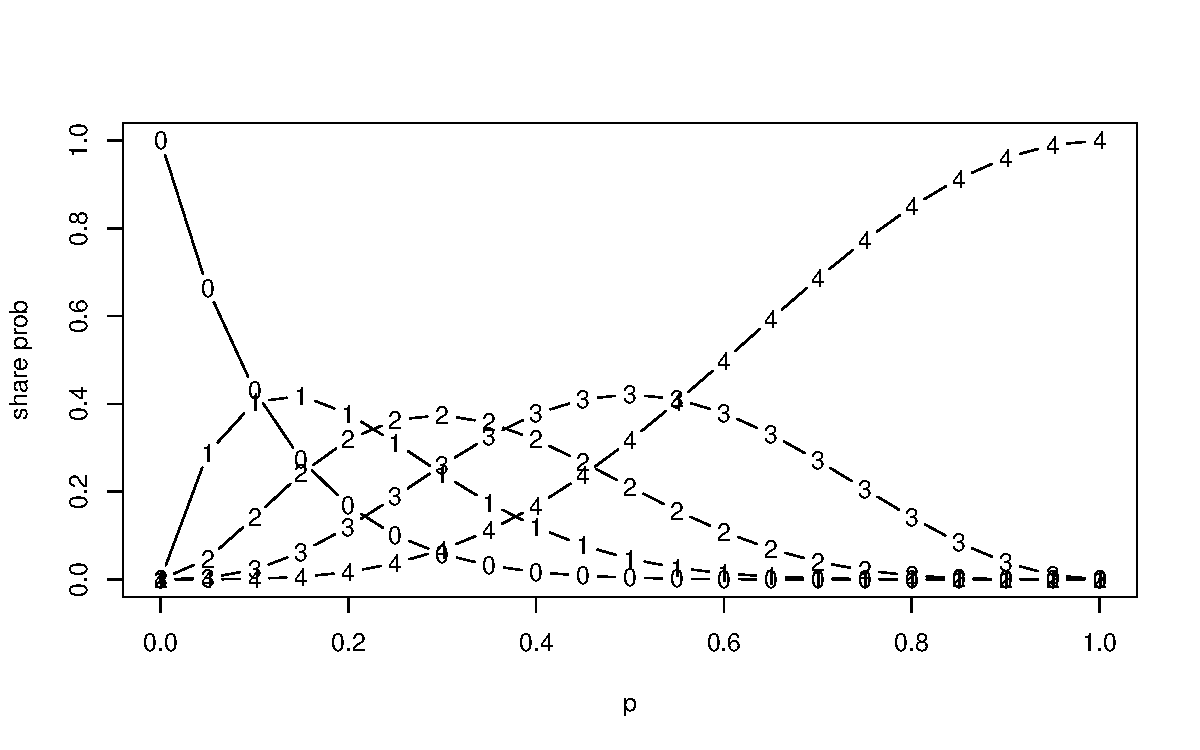
\includegraphics[width=\maxwidth]{/homes/gws/ruzzo/Documents/g/projects/thaps/Thaps_7_strains/scripts/larrys/shared-snps/figs-knitr/share-plot-1} 

}

\caption[Sharing Probability]{Sharing Probability}\label{fig:share-plot}
\end{figure}


\end{knitrout}

\subsection{Old Tree Stuff}

All based on un-q-filtered reads.

The first pass at the tree analysis was the Chr1 tree, \emph{loose criteria} (c1); it is rendered via \\{\small\tt http://iubio.bio.indiana.edu/treeapp/treeprint-form.html} as Fig~\ref{fig:tree-v1}, and in newick format is:

%\noindent {\footnotesize\begin{verbatim}
%(((tp3367_Italy:4551,tp1013_Wales:4954):5920,(((tp1007_Virginia:10,tp1012_Australia:29):9,
%(tp1015_Puget_Sound:90,tp1335_NY:13):11):320,tp1014_Gyre:22):3484):8593);
%\end{verbatim}}
\begin{knitrout}\footnotesize
\definecolor{shadecolor}{rgb}{0.969, 0.969, 0.969}\color{fgcolor}\begin{kframe}
\begin{alltt}
\hlstd{newick.chr1.loose} \hlkwb{<-} \hlstr{'(((tp3367_Italy:4551,tp1013_Wales:4954):5920,(((tp1007_Virginia:10,tp1012_Australia:29):9,(tp1015_Puget_Sound:90,tp1335_NY:13):11):320,tp1014_Gyre:22):3484):8593,outgroup:0);'}
\hlkwd{cat.hardwrap}\hlstd{(newick.chr1.loose)}
\end{alltt}
\begin{verbatim}
# (((tp3367_Italy:4551,tp1013_Wales:4954):5920,(((tp1007_Virginia:10,tp1012_Austra 
# lia:29):9,(tp1015_Puget_Sound:90,tp1335_NY:13):11):320,tp1014_Gyre:22):3484):859 
# 3,outgroup:0);
\end{verbatim}
\end{kframe}
\end{knitrout}

\begin{figure}
  \begin{center}
    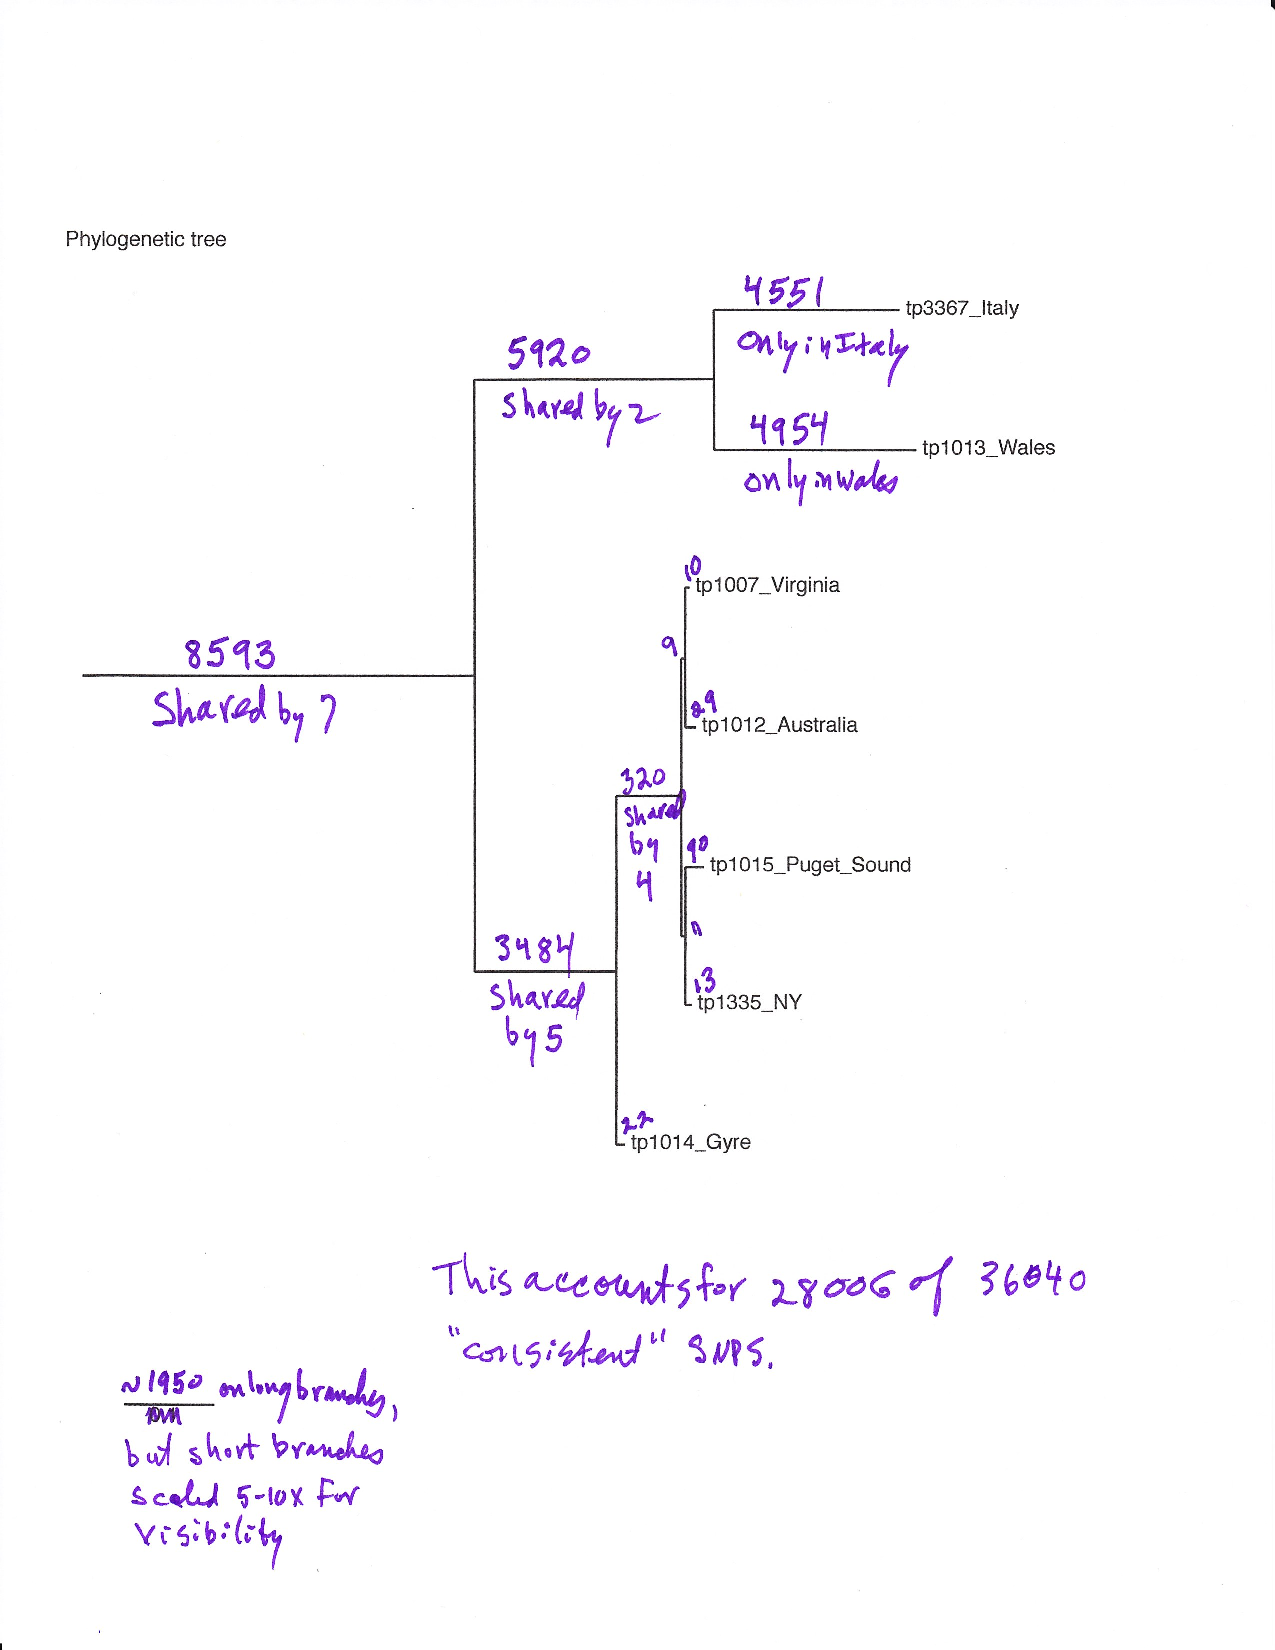
\includegraphics[scale=.5]{00old/shared-snp-tree-annotated-v1.pdf}
    \caption{Inferred Tree, based on Chr1, un-q-filtered reads, loose criteria.  (Note: to visually resolve the edges among the
      5, their lengths were scaled by 5x -- 10x in this figure, but not in the newick description
      shown in the text.)}
    \label{fig:tree-v1}
  \end{center}
\end{figure}

Chr 1 tree based on \emph{medium criteria} (c2) has exactly the same topology is, although the 
branch lengths are different.  As noted earlier, the length of the branch labeled ``*'' is probably
inflated by lower coverage and higher error rate in 1014, which may mask further legitimate sharing 
between it and the other L-isloates.  The branch lengths among the other 4 are too short for its 
topology to be convincing without a more rigorous analysis (e.g., a bootstrap test).

Chr1 tree, medium criteria, in newick format:

\begin{knitrout}\footnotesize
\definecolor{shadecolor}{rgb}{0.969, 0.969, 0.969}\color{fgcolor}\begin{kframe}
\begin{alltt}
\hlstd{newick.chr1.med} \hlkwb{<-} \hlstr{'(((tp3367_Italy:8813,tp1013_Wales:9652):9365,(((e_tp1007_Virginia:30,d_tp1012_Australia:61):19,(c_tp1015_Puget_Sound:207,b_tp1335_NY:41):18):1005,a_tp1014_Gyre:61):3912):7054,outgroup:0);'}
\hlkwd{cat.hardwrap}\hlstd{(newick.chr1.med)}
\end{alltt}
\begin{verbatim}
# (((tp3367_Italy:8813,tp1013_Wales:9652):9365,(((e_tp1007_Virginia:30,d_tp1012_Au 
# stralia:61):19,(c_tp1015_Puget_Sound:207,b_tp1335_NY:41):18):1005,a_tp1014_Gyre: 
# 61):3912):7054,outgroup:0);
\end{verbatim}
\end{kframe}
\end{knitrout}

NOTE: In early code, tree was not being recalculated; it was defined by constants in the following 
code chunk, hand-copied from the analysis above.  

\begin{knitrout}\scriptsize
\definecolor{shadecolor}{rgb}{0.969, 0.969, 0.969}\color{fgcolor}\begin{kframe}
\begin{alltt}
\hlcom{# tree parameters as nested lists }
\hlcom{#   Internal nodes have subtrees sub1/2 and length}
\hlcom{#   Root has sub1/2, but no length}
\hlcom{#   Leaves have where, length, optionally, id, alt, nb.  (Omit id for 'outgroup'. Use 'alt' for less formal}
\hlcom{#     labeling in cartoon version; it defaults to 'where'. Use 'nb' to add abcde annotations for legend.)}
\hlcom{# This hand-made version is now subsumed by make.tree; retained for comparison}
\hlstd{tree.by.hand} \hlkwb{<-}
  \hlkwd{list}\hlstd{(}
    \hlkwc{sub1} \hlstd{=} \hlkwd{list}\hlstd{(}
      \hlkwc{sub1} \hlstd{=} \hlkwd{list}\hlstd{(}
        \hlkwc{sub1} \hlstd{=} \hlkwd{list}\hlstd{(}\hlkwc{id}\hlstd{=}\hlnum{3367}\hlstd{,} \hlkwc{length}\hlstd{=}\hlnum{8813}\hlstd{,} \hlkwc{where}\hlstd{=}\hlstr{'Venice, Italy'}\hlstd{,} \hlkwc{alt}\hlstd{=}\hlstr{'Venice'}\hlstd{),}
        \hlkwc{sub2} \hlstd{=} \hlkwd{list}\hlstd{(}\hlkwc{id}\hlstd{=}\hlnum{1013}\hlstd{,} \hlkwc{length}\hlstd{=}\hlnum{9652}\hlstd{,} \hlkwc{where}\hlstd{=}\hlstr{'Wales, UK'}\hlstd{),}
        \hlkwc{length}\hlstd{=}\hlnum{9365}\hlstd{),}
      \hlkwc{sub2} \hlstd{=}  \hlkwd{list}\hlstd{(}
        \hlkwc{sub1} \hlstd{=} \hlkwd{list}\hlstd{(}
          \hlkwc{sub1} \hlstd{=} \hlkwd{list}\hlstd{(}
            \hlkwc{sub1} \hlstd{=} \hlkwd{list}\hlstd{(}\hlkwc{id}\hlstd{=}\hlnum{1007}\hlstd{,} \hlkwc{length}\hlstd{=}\hlnum{30}\hlstd{,} \hlkwc{nb}\hlstd{=}\hlstr{'e'}\hlstd{,} \hlkwc{where}\hlstd{=}\hlstr{'Virginia, USA'}\hlstd{),}
            \hlkwc{sub2} \hlstd{=} \hlkwd{list}\hlstd{(}\hlkwc{id}\hlstd{=}\hlnum{1012}\hlstd{,} \hlkwc{length}\hlstd{=}\hlnum{61}\hlstd{,} \hlkwc{nb}\hlstd{=}\hlstr{'d'}\hlstd{,} \hlkwc{where}\hlstd{=}\hlstr{'Perth, W. Australia'}\hlstd{,} \hlkwc{alt}\hlstd{=}\hlstr{'Perth'}\hlstd{),}
            \hlkwc{length}\hlstd{=}\hlnum{19}\hlstd{),}
          \hlkwc{sub2} \hlstd{=} \hlkwd{list}\hlstd{(}
            \hlkwc{sub1} \hlstd{=} \hlkwd{list}\hlstd{(}\hlkwc{id}\hlstd{=}\hlnum{1015}\hlstd{,} \hlkwc{length}\hlstd{=}\hlnum{207}\hlstd{,}\hlkwc{nb}\hlstd{=}\hlstr{'c'}\hlstd{,} \hlkwc{where}\hlstd{=}\hlstr{'Washington, USA'}\hlstd{,} \hlkwc{alt}\hlstd{=}\hlstr{'Puget Sound'}\hlstd{),}
            \hlkwc{sub2} \hlstd{=} \hlkwd{list}\hlstd{(}\hlkwc{id}\hlstd{=}\hlnum{1335}\hlstd{,} \hlkwc{length}\hlstd{=}\hlnum{41}\hlstd{,} \hlkwc{nb}\hlstd{=}\hlstr{'b'}\hlstd{,} \hlkwc{where}\hlstd{=}\hlstr{'New York, USA'}\hlstd{,}   \hlkwc{alt}\hlstd{=}\hlstr{'NY'}\hlstd{),}
            \hlkwc{length}\hlstd{=}\hlnum{18}\hlstd{),}
          \hlkwc{length}\hlstd{=}\hlnum{1005}\hlstd{),}
        \hlkwc{sub2} \hlstd{=} \hlkwd{list}\hlstd{(}\hlkwc{id}\hlstd{=}\hlnum{1014}\hlstd{,} \hlkwc{length}\hlstd{=}\hlnum{61}\hlstd{,} \hlkwc{nb}\hlstd{=}\hlstr{'a'}\hlstd{,} \hlkwc{where}\hlstd{=}\hlstr{'N. Pacific Gyre'}\hlstd{),}
        \hlkwc{length}\hlstd{=}\hlnum{3912}\hlstd{),}
      \hlkwc{length}\hlstd{=}\hlnum{7054}\hlstd{),}
    \hlkwc{sub2} \hlstd{=} \hlkwd{list}\hlstd{(}\hlkwc{length}\hlstd{=}\hlnum{0}\hlstd{,} \hlkwc{where}\hlstd{=}\hlstr{'outgroup'}\hlstd{)}
  \hlstd{)}

\hlcom{# historical, format example, and debug help:}
\hlstd{oldwick.medium} \hlkwb{<-} \hlstr{'(((CCMP3367_Italy:8813,CCMP1013_Wales:9652):9365,(((e_CCMP1007_Virginia:30,d_CCMP1012_Australia:61):19,(c_CCMP1015_Puget_Sound:207,b_CCMP1335_NY:41):18):1005,a_CCMP1014_NPG:61):3912):7054,outgroup:0);'}
\hlcom{# with simpler labeling for cartoon}
\hlstd{simple.oldwick.medium} \hlkwb{<-} \hlstr{'(((Italy:8813,Wales:9652):9365,(((Virginia:30,Australia:61):19,(Puget:207,NY:41):18):1005,Gyre:61):3912):7054,outgroup:0);'}
\hlkwd{cat.hardwrap}\hlstd{(oldwick.medium)}
\end{alltt}
\begin{verbatim}
# (((CCMP3367_Italy:8813,CCMP1013_Wales:9652):9365,(((e_CCMP1007_Virginia:30,d_CCM 
# P1012_Australia:61):19,(c_CCMP1015_Puget_Sound:207,b_CCMP1335_NY:41):18):1005,a_ 
# CCMP1014_NPG:61):3912):7054,outgroup:0);
\end{verbatim}
\begin{alltt}
\hlkwd{cat.hardwrap}\hlstd{(simple.oldwick.medium)}
\end{alltt}
\begin{verbatim}
# (((Italy:8813,Wales:9652):9365,(((Virginia:30,Australia:61):19,(Puget:207,NY:41) 
# :18):1005,Gyre:61):3912):7054,outgroup:0);
\end{verbatim}
\end{kframe}
\end{knitrout}

Two other versions of the tree, for possible use in figs in the main paper.

Figure~\ref{fig:tree-medium-unlabeled}:  [** as of 10/4/2015, this fig and next have stray stars on virginia, wales labels; probably due to hacking with commas in newick; not worth fixing unless we resurrect these trees for some purpose, but if so, see use of newick.name.undo in show.tree as probable fix. **]

\begin{knitrout}\scriptsize
\definecolor{shadecolor}{rgb}{0.969, 0.969, 0.969}\color{fgcolor}\begin{kframe}
\begin{alltt}
\hlstd{tree.scale} \hlkwb{<-} \hlkwd{ifelse}\hlstd{(}\hlkwd{which.snp.tables}\hlstd{(}\hlkwc{string.val}\hlstd{=F)[}\hlnum{1}\hlstd{]}\hlopt{==}\hlstr{'Chr1'}\hlstd{,} \hlnum{1}\hlstd{,} \hlnum{10}\hlstd{)}
\hlstd{tree.x.lim} \hlkwb{<-} \hlnum{3e4} \hlopt{*} \hlstd{tree.scale}
\hlstd{the.simple.tree} \hlkwb{<-} \hlkwd{read.tree}\hlstd{(}\hlkwc{text}\hlstd{=simple.newick.medium)}
\hlkwd{plot}\hlstd{(the.simple.tree,} \hlkwc{x.lim} \hlstd{= tree.x.lim)}
\hlkwd{axis}\hlstd{(}\hlnum{1}\hlstd{)}
\end{alltt}
\end{kframe}\begin{figure}

{\centering 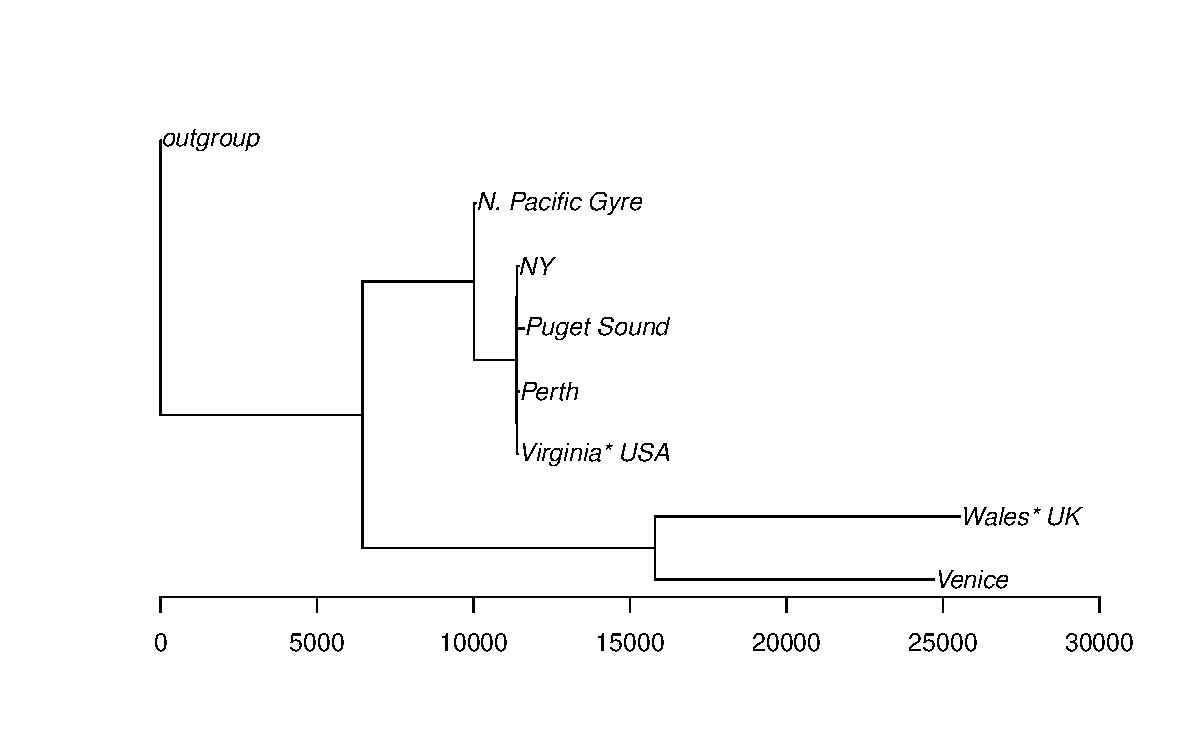
\includegraphics[width=3.5in]{/homes/gws/ruzzo/Documents/g/projects/thaps/Thaps_7_strains/scripts/larrys/shared-snps/figs-knitr/newick-Chr1-qfiltered-tree-medium-unlabeled-1} 

}

\caption[Tree based on qfiltered reads and medium SNP filters]{Tree based on qfiltered reads and medium SNP filters.  ``Lengths'' are numbers of shared/private SNPs on Chr1. (no edge labels, nolegend)}\label{fig:tree-medium-unlabeled}
\end{figure}


\end{knitrout}

Figure~\ref{fig:tree-medium-unlabeled-shortscale}:

\begin{knitrout}\scriptsize
\definecolor{shadecolor}{rgb}{0.969, 0.969, 0.969}\color{fgcolor}\begin{kframe}
\begin{alltt}
\hlkwd{plot}\hlstd{(the.simple.tree,} \hlkwc{x.lim} \hlstd{= tree.x.lim)}
\hlkwd{axis}\hlstd{(}\hlnum{1}\hlstd{,(}\hlnum{0}\hlopt{:}\hlnum{4}\hlstd{)}\hlopt{*}\hlnum{7000}\hlopt{*}\hlstd{tree.scale,(}\hlnum{0}\hlopt{:}\hlnum{4}\hlstd{)}\hlopt{*}\hlnum{7000}\hlopt{*}\hlstd{tree.scale)}
\end{alltt}
\end{kframe}\begin{figure}

{\centering 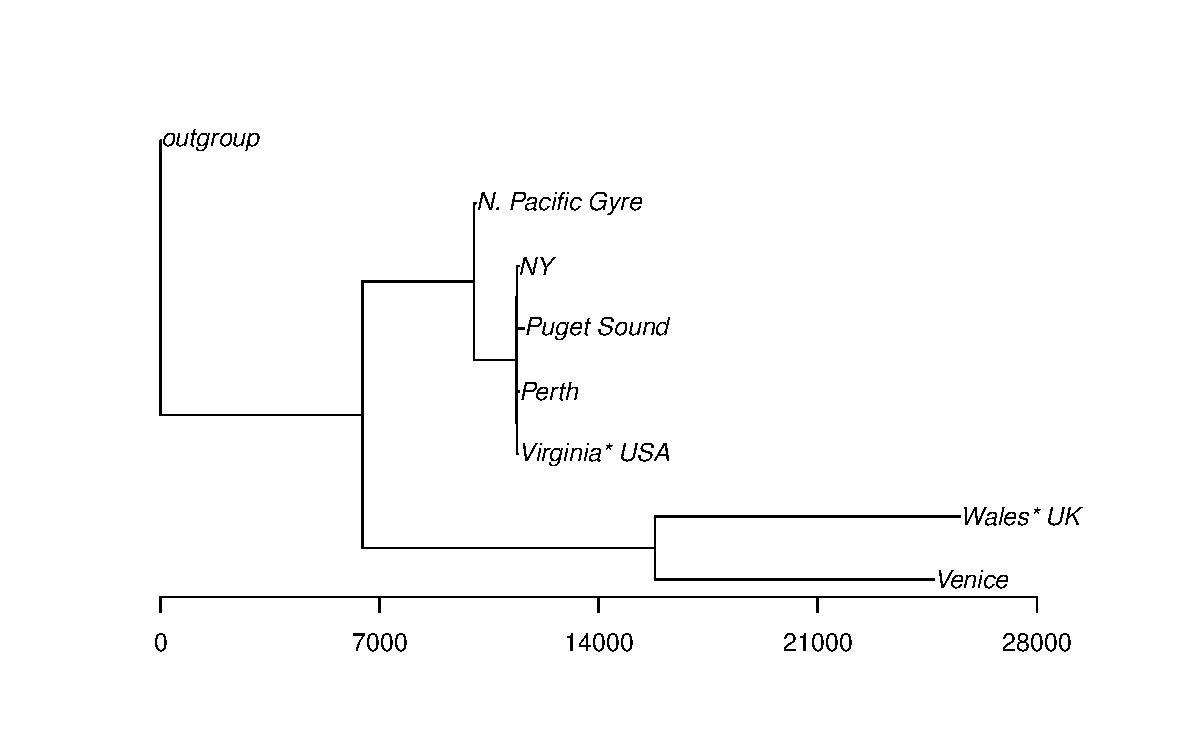
\includegraphics[width=3.5in]{/homes/gws/ruzzo/Documents/g/projects/thaps/Thaps_7_strains/scripts/larrys/shared-snps/figs-knitr/newick-Chr1-qfiltered-tree-medium-unlabeled-shortscale-1} 

}

\caption[Tree based on qfiltered reads and medium SNP filters]{Tree based on qfiltered reads and medium SNP filters.  ``Lengths'' are numbers of shared/private SNPs on Chr1. (no edge labels, no legend, short scale bar)}\label{fig:tree-medium-unlabeled-shortscale}
\end{figure}


\end{knitrout}

At some much earlier point, Tony ran the whole-genome version of the then-current code above, and manually entered tree branch lengths/legend for the resuting tree, shown in Fig~\ref{fig:fullgenome-tree-medium}.  Code above can now automatically generate such a tree, but retain the following for comparison.  The basic story seems clear---same topology and branch lengths scaled by about 10x, which is completely reasonable given that Chr1 is about 10\% of the genome.  Note that this tree is not being recalculated; it is defined by constants in the following code chunk.

\begin{knitrout}\scriptsize
\definecolor{shadecolor}{rgb}{0.969, 0.969, 0.969}\color{fgcolor}\begin{kframe}
\begin{alltt}
\hlstd{fullgenome.newick.medium} \hlkwb{<-} \hlstr{'(((3367_Italy:86155,1013_Wales:95697):89598,(((e_1007_VA:330,d_1012_Australia:632):1296,(c_1015_WA:2113,b_1335_NY:658):480):10059,a_1014_NPG:568):39517):69526,outgroup:0);'}
\hlkwd{cat.hardwrap}\hlstd{(fullgenome.newick.medium)}
\end{alltt}
\begin{verbatim}
# (((3367_Italy:86155,1013_Wales:95697):89598,(((e_1007_VA:330,d_1012_Australia:63 
# 2):1296,(c_1015_WA:2113,b_1335_NY:658):480):10059,a_1014_NPG:568):39517):69526,o 
# utgroup:0);
\end{verbatim}
\begin{alltt}
\hlstd{legend.text} \hlkwb{<-} \hlkwd{c}\hlstd{(}\hlstr{'a: only in 1014  '}\hlstd{,}
                 \hlstr{'b: only in 1335  '}\hlstd{,}
                 \hlstr{'c: only in 1015  '}\hlstd{,}
                 \hlstr{'d: only in 1012  '}\hlstd{,}
                 \hlstr{'e: only in 1007  '}\hlstd{,}
                 \hlstr{'*: shared by bcde'}\hlstd{,}
                 \hlstr{'   shared by b/c '}\hlstd{,}
                 \hlstr{'   shared by d/e '}
\hlstd{)}
\hlstd{fullgenome.tree.x.lim} \hlkwb{<-} \hlnum{300000}
\hlstd{fullgenome.counts} \hlkwb{<-} \hlkwd{c}\hlstd{(} \hlnum{568}\hlstd{,} \hlnum{658}\hlstd{,} \hlnum{2113}\hlstd{,} \hlnum{632}\hlstd{,} \hlnum{330}\hlstd{,} \hlnum{10059}\hlstd{,} \hlnum{480}\hlstd{,} \hlnum{1296} \hlstd{)}
\hlstd{fullgenome.legend.text} \hlkwb{<-} \hlkwd{paste}\hlstd{(legend.text,}\hlkwd{format}\hlstd{(fullgenome.counts,}\hlkwc{width}\hlstd{=}\hlnum{5}\hlstd{),}\hlkwc{sep}\hlstd{=}\hlstr{' - '}\hlstd{)}
\hlstd{fullgenome.tree.labels} \hlkwb{<-} \hlkwd{list}\hlstd{(} \hlcom{## x,y,text}
     \hlnum{41000}\hlstd{,}\hlnum{3.63}\hlstd{,}\hlstr{'69526\textbackslash{}nshared by 7'}\hlstd{,}
     \hlnum{90000}\hlstd{,}\hlnum{5.75}\hlstd{,}\hlstr{'39517\textbackslash{}nby 5 (**)'}\hlstd{,}
    \hlnum{115000}\hlstd{,}\hlnum{1.5}\hlstd{,} \hlstr{'89598\textbackslash{}nshared by 2'}\hlstd{,}
    \hlnum{210000}\hlstd{,}\hlnum{2.0}\hlstd{,} \hlstr{'95697 only\textbackslash{}nin Wales'}\hlstd{,}
    \hlnum{210000}\hlstd{,}\hlnum{1.0}\hlstd{,} \hlstr{'86155 only\textbackslash{}nin Italy'}\hlstd{,}
    \hlnum{113500}\hlstd{,}\hlnum{4.6}\hlstd{,} \hlstr{'*'}\hlstd{)}
\end{alltt}
\end{kframe}
\end{knitrout}

Figure~\ref{fig:fullgenome-tree-medium}:

\begin{knitrout}\scriptsize
\definecolor{shadecolor}{rgb}{0.969, 0.969, 0.969}\color{fgcolor}\begin{kframe}
\begin{alltt}
\hlkwd{library}\hlstd{(ape)}
\hlstd{the.fullgenome.tree} \hlkwb{<-} \hlkwd{read.tree}\hlstd{(}\hlkwc{text}\hlstd{=fullgenome.newick.medium)}
\hlkwd{plot}\hlstd{(the.fullgenome.tree,} \hlkwc{x.lim} \hlstd{= fullgenome.tree.x.lim)}
\hlkwd{axis}\hlstd{(}\hlnum{1}\hlstd{)} \hlcom{# ; axis(2) useful only for placing labels}
\hlstd{opar} \hlkwb{<-} \hlkwd{par}\hlstd{(}\hlkwc{family}\hlstd{=}\hlstr{'mono'}\hlstd{,}\hlkwc{cex}\hlstd{=}\hlnum{.8}\hlstd{)}
\hlkwd{legend}\hlstd{(}\hlstr{'topright'}\hlstd{,} \hlkwc{legend}\hlstd{=fullgenome.legend.text)}
\hlkwd{par}\hlstd{(opar)}
\hlkwa{for}\hlstd{(i} \hlkwa{in} \hlkwd{seq}\hlstd{(}\hlnum{1}\hlstd{,}\hlkwd{length}\hlstd{(fullgenome.tree.labels)}\hlopt{-}\hlnum{2}\hlstd{,}\hlkwc{by}\hlstd{=}\hlnum{3}\hlstd{))\{}
  \hlkwd{text}\hlstd{(fullgenome.tree.labels[[i]], fullgenome.tree.labels[[i}\hlopt{+}\hlnum{1}\hlstd{]], fullgenome.tree.labels[[i}\hlopt{+}\hlnum{2}\hlstd{]])}
\hlstd{\}}
\end{alltt}
\end{kframe}\begin{figure}

{\centering 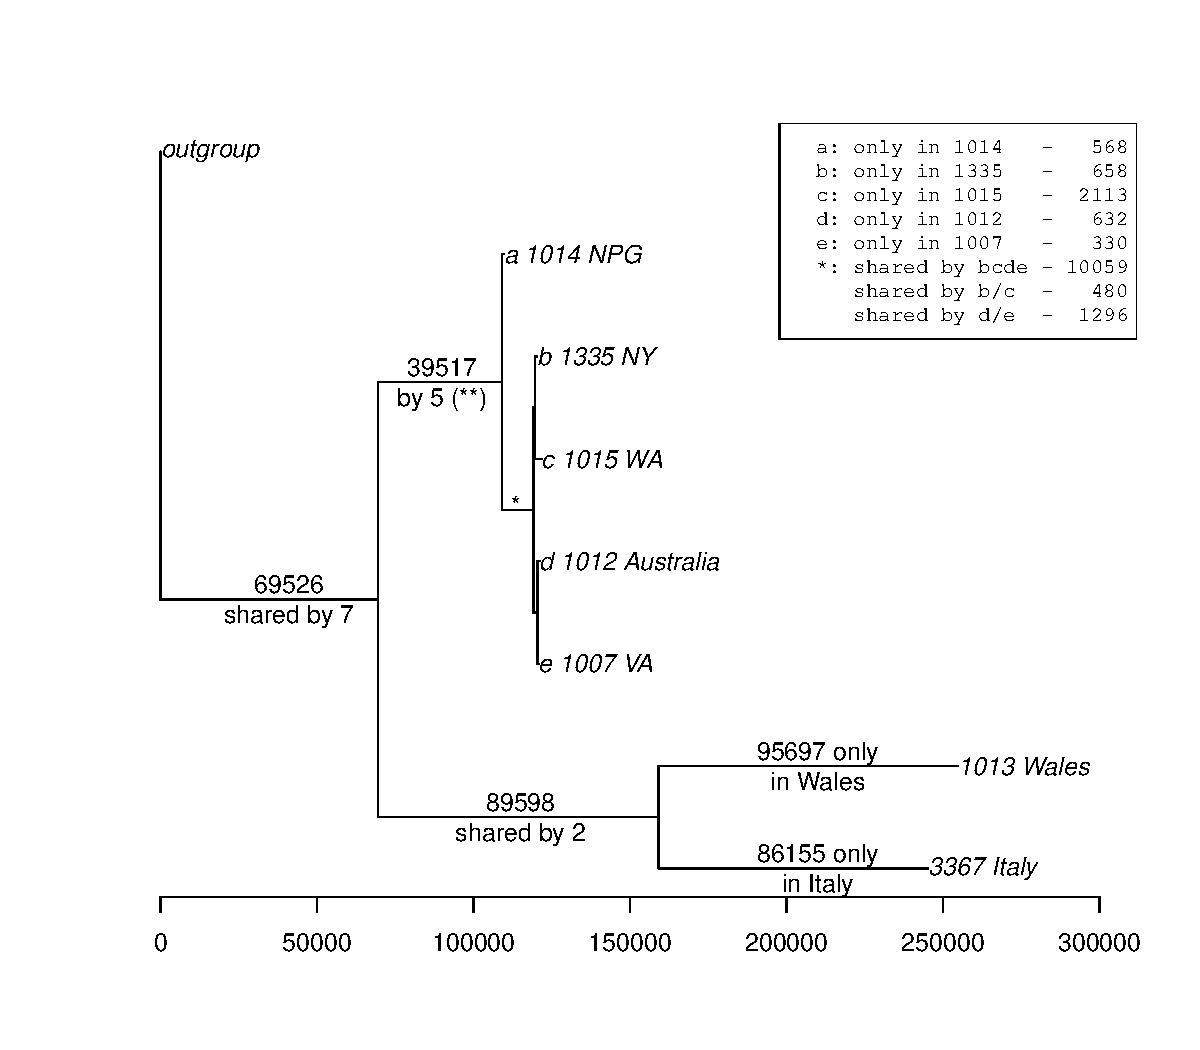
\includegraphics[width=\maxwidth]{/homes/gws/ruzzo/Documents/g/projects/thaps/Thaps_7_strains/scripts/larrys/shared-snps/figs-knitr/fullgenome-tree-medium-1} 

}

\caption[Tree based on unqfiltered reads and medium SNP filters]{Tree based on unqfiltered reads and medium SNP filters.  ``Lengths'' are numbers of shared/private SNPs genome-wide. (By-hand legacy version)}\label{fig:fullgenome-tree-medium}
\end{figure}


\end{knitrout}

\FloatBarrier

% remember to do this to enable Id keyword substution: svn propset svn:keywords Id shared-snps.rnw 
\mbox{}\vfill\footnotesize\flushright SVN, ID I miss you.\ $ $Id: shared-snps.rnw  2017-07-21 or later. ruzzo $ $
\end{document}
